\documentclass[twoside]{book}

% Packages required by doxygen
\usepackage{fixltx2e}
\usepackage{calc}
\usepackage{doxygen}
\usepackage[export]{adjustbox} % also loads graphicx
\usepackage{graphicx}
\usepackage[utf8]{inputenc}
\usepackage{makeidx}
\usepackage{multicol}
\usepackage{multirow}
\PassOptionsToPackage{warn}{textcomp}
\usepackage{textcomp}
\usepackage[nointegrals]{wasysym}
\usepackage[table]{xcolor}

% Font selection
\usepackage[T1]{fontenc}
\usepackage[scaled=.90]{helvet}
\usepackage{courier}
\usepackage{amssymb}
\usepackage{sectsty}
\renewcommand{\familydefault}{\sfdefault}
\allsectionsfont{%
  \fontseries{bc}\selectfont%
  \color{darkgray}%
}
\renewcommand{\DoxyLabelFont}{%
  \fontseries{bc}\selectfont%
  \color{darkgray}%
}
\newcommand{\+}{\discretionary{\mbox{\scriptsize$\hookleftarrow$}}{}{}}

% Page & text layout
\usepackage{geometry}
\geometry{%
  a4paper,%
  top=2.5cm,%
  bottom=2.5cm,%
  left=2.5cm,%
  right=2.5cm%
}
\tolerance=750
\hfuzz=15pt
\hbadness=750
\setlength{\emergencystretch}{15pt}
\setlength{\parindent}{0cm}
\setlength{\parskip}{0.2cm}
\makeatletter
\renewcommand{\paragraph}{%
  \@startsection{paragraph}{4}{0ex}{-1.0ex}{1.0ex}{%
    \normalfont\normalsize\bfseries\SS@parafont%
  }%
}
\renewcommand{\subparagraph}{%
  \@startsection{subparagraph}{5}{0ex}{-1.0ex}{1.0ex}{%
    \normalfont\normalsize\bfseries\SS@subparafont%
  }%
}
\makeatother

% Headers & footers
\usepackage{fancyhdr}
\pagestyle{fancyplain}
\fancyhead[LE]{\fancyplain{}{\bfseries\thepage}}
\fancyhead[CE]{\fancyplain{}{}}
\fancyhead[RE]{\fancyplain{}{\bfseries\leftmark}}
\fancyhead[LO]{\fancyplain{}{\bfseries\rightmark}}
\fancyhead[CO]{\fancyplain{}{}}
\fancyhead[RO]{\fancyplain{}{\bfseries\thepage}}
\fancyfoot[LE]{\fancyplain{}{}}
\fancyfoot[CE]{\fancyplain{}{}}
\fancyfoot[RE]{\fancyplain{}{\bfseries\scriptsize Generated on Fri Sep 4 2015 22\+:11\+:14 for Tina4 by Doxygen }}
\fancyfoot[LO]{\fancyplain{}{\bfseries\scriptsize Generated on Fri Sep 4 2015 22\+:11\+:14 for Tina4 by Doxygen }}
\fancyfoot[CO]{\fancyplain{}{}}
\fancyfoot[RO]{\fancyplain{}{}}
\renewcommand{\footrulewidth}{0.4pt}
\renewcommand{\chaptermark}[1]{%
  \markboth{#1}{}%
}
\renewcommand{\sectionmark}[1]{%
  \markright{\thesection\ #1}%
}

% Indices & bibliography
\usepackage{natbib}
\usepackage[titles]{tocloft}
\setcounter{tocdepth}{3}
\setcounter{secnumdepth}{5}
\makeindex

% Hyperlinks (required, but should be loaded last)
\usepackage{ifpdf}
\ifpdf
  \usepackage[pdftex,pagebackref=true]{hyperref}
\else
  \usepackage[ps2pdf,pagebackref=true]{hyperref}
\fi
\hypersetup{%
  colorlinks=true,%
  linkcolor=blue,%
  citecolor=blue,%
  unicode%
}

% Custom commands
\newcommand{\clearemptydoublepage}{%
  \newpage{\pagestyle{empty}\cleardoublepage}%
}


%===== C O N T E N T S =====

\begin{document}

% Titlepage & ToC
\hypersetup{pageanchor=false,
             bookmarks=true,
             bookmarksnumbered=true,
             pdfencoding=unicode
            }
\pagenumbering{roman}
\begin{titlepage}
\vspace*{7cm}
\begin{center}%
{\Large Tina4 }\\
\vspace*{1cm}
{\large Generated by Doxygen 1.8.9.1}\\
\vspace*{0.5cm}
{\small Fri Sep 4 2015 22:11:14}\\
\end{center}
\end{titlepage}
\clearemptydoublepage
\tableofcontents
\clearemptydoublepage
\pagenumbering{arabic}
\hypersetup{pageanchor=true}

%--- Begin generated contents ---
\chapter{Todo List}
\label{todo}
\hypertarget{todo}{}

\begin{DoxyRefList}
\item[\label{todo__todo000001}%
\hypertarget{todo__todo000001}{}%
Member \hyperlink{classCody_a91baebb215438e27a00b211a2e352b14}{Cody\+:\+:boot\+Strap\+Tabs} (\$tabs=array())]generate unique id identifier for tab ids 
\begin{DoxyParams}[1]{Parameters}
array & {\em \$tabs} & \\
\hline
\end{DoxyParams}
\begin{DoxyReturn}{Returns}
string 
\end{DoxyReturn}

\item[\label{todo__todo000002}%
\hypertarget{todo__todo000002}{}%
Member \hyperlink{classDebby_a482145f057ea4b31d4414d0ea8997244}{Debby\+:\+:update} (\$tablename, \$field\+Values, \$index\+Field\+Value)]prevent updating if index\+Field\+Value is empty  
\item[\label{todo__todo000003}%
\hypertarget{todo__todo000003}{}%
Class \hyperlink{classEmma}{Emma} ]Add the ability to parse email addresses 
\item[\label{todo__todo000004}%
\hypertarget{todo__todo000004}{}%
Member \hyperlink{classEmma_a41ce44cec1c4b79421b8fe2f0c9dc6b6}{Emma\+:\+:\+\_\+\+\_\+construct} (\$bulk\+S\+M\+S\+Username=\char`\"{}\char`\"{}, \$bulk\+S\+M\+S\+Password=\char`\"{}\char`\"{})]Add the ability to talk to a specific email server 
\end{DoxyRefList}
\chapter{Namespace Index}
\section{Namespace List}
Here is a list of all namespaces with brief descriptions\+:\begin{DoxyCompactList}
\item\contentsline{section}{\hyperlink{namespaceJSMin}{J\+S\+Min} }{\pageref{namespaceJSMin}}{}
\end{DoxyCompactList}

\chapter{Hierarchical Index}
\section{Class Hierarchy}
This inheritance list is sorted roughly, but not completely, alphabetically\+:\begin{DoxyCompactList}
\item \contentsline{section}{Cody}{\pageref{classCody}}{}
\item \contentsline{section}{Debby}{\pageref{classDebby}}{}
\item \contentsline{section}{Emma}{\pageref{classEmma}}{}
\item Exception\begin{DoxyCompactList}
\item \contentsline{section}{J\+S\+Min\+\_\+\+Unterminated\+Comment\+Exception}{\pageref{classJSMin__UnterminatedCommentException}}{}
\item \contentsline{section}{J\+S\+Min\+\_\+\+Unterminated\+Reg\+Exp\+Exception}{\pageref{classJSMin__UnterminatedRegExpException}}{}
\item \contentsline{section}{J\+S\+Min\+\_\+\+Unterminated\+String\+Exception}{\pageref{classJSMin__UnterminatedStringException}}{}
\end{DoxyCompactList}
\item \contentsline{section}{Glocell}{\pageref{classGlocell}}{}
\item Iterator\begin{DoxyCompactList}
\item \contentsline{section}{Olga}{\pageref{classOlga}}{}
\end{DoxyCompactList}
\item \contentsline{section}{J\+S\+Min}{\pageref{classJSMin}}{}
\item \contentsline{section}{Kim}{\pageref{classKim}}{}
\item \contentsline{section}{Maggy}{\pageref{classMaggy}}{}
\item \contentsline{section}{Phoebe}{\pageref{classPhoebe}}{}
\item \contentsline{section}{Reta}{\pageref{classReta}}{}
\item \contentsline{section}{Ruth}{\pageref{classRuth}}{}
\item \contentsline{section}{shape\+Base\+Element}{\pageref{classshapeBaseElement}}{}
\begin{DoxyCompactList}
\item \contentsline{section}{html\+Element}{\pageref{classhtmlElement}}{}
\end{DoxyCompactList}
\item \contentsline{section}{Tessa}{\pageref{classTessa}}{}
\item \contentsline{section}{test\+Class}{\pageref{classtestClass}}{}
\item \contentsline{section}{Test\+Element}{\pageref{classTestElement}}{}
\end{DoxyCompactList}

\chapter{Class Index}
\section{Class List}
Here are the classes, structs, unions and interfaces with brief descriptions\+:\begin{DoxyCompactList}
\item\contentsline{section}{\hyperlink{classCody}{Cody} }{\pageref{classCody}}{}
\item\contentsline{section}{\hyperlink{classDebby}{Debby} }{\pageref{classDebby}}{}
\item\contentsline{section}{\hyperlink{classEmma}{Emma} }{\pageref{classEmma}}{}
\item\contentsline{section}{\hyperlink{classhtmlElement}{html\+Element} }{\pageref{classhtmlElement}}{}
\item\contentsline{section}{\hyperlink{classJSMin}{J\+S\+Min} }{\pageref{classJSMin}}{}
\item\contentsline{section}{\hyperlink{classJSMin__UnterminatedCommentException}{J\+S\+Min\+\_\+\+Unterminated\+Comment\+Exception} }{\pageref{classJSMin__UnterminatedCommentException}}{}
\item\contentsline{section}{\hyperlink{classJSMin__UnterminatedRegExpException}{J\+S\+Min\+\_\+\+Unterminated\+Reg\+Exp\+Exception} }{\pageref{classJSMin__UnterminatedRegExpException}}{}
\item\contentsline{section}{\hyperlink{classJSMin__UnterminatedStringException}{J\+S\+Min\+\_\+\+Unterminated\+String\+Exception} }{\pageref{classJSMin__UnterminatedStringException}}{}
\item\contentsline{section}{\hyperlink{classKim}{Kim} }{\pageref{classKim}}{}
\item\contentsline{section}{\hyperlink{classMaggy}{Maggy} }{\pageref{classMaggy}}{}
\item\contentsline{section}{\hyperlink{classOlga}{Olga} }{\pageref{classOlga}}{}
\item\contentsline{section}{\hyperlink{classPhoebe}{Phoebe} }{\pageref{classPhoebe}}{}
\item\contentsline{section}{\hyperlink{classReta}{Reta} }{\pageref{classReta}}{}
\item\contentsline{section}{\hyperlink{classRuth}{Ruth} }{\pageref{classRuth}}{}
\item\contentsline{section}{\hyperlink{classshapeBaseElement}{shape\+Base\+Element} }{\pageref{classshapeBaseElement}}{}
\item\contentsline{section}{\hyperlink{classTessa}{Tessa} }{\pageref{classTessa}}{}
\item\contentsline{section}{\hyperlink{classtestClass}{test\+Class} }{\pageref{classtestClass}}{}
\item\contentsline{section}{\hyperlink{classTestElement}{Test\+Element} }{\pageref{classTestElement}}{}
\end{DoxyCompactList}

\chapter{File Index}
\section{File List}
Here is a list of all files with brief descriptions\+:\begin{DoxyCompactList}
\item\contentsline{section}{web\+\_\+root/\hyperlink{tina4_8php}{tina4.\+php} }{\pageref{tina4_8php}}{}
\item\contentsline{section}{web\+\_\+root/project/\hyperlink{Glocell_8php}{Glocell.\+php} }{\pageref{Glocell_8php}}{}
\item\contentsline{section}{web\+\_\+root/project/\hyperlink{testClass_8php}{test\+Class.\+php} }{\pageref{testClass_8php}}{}
\item\contentsline{section}{web\+\_\+root/tina4/\hyperlink{Cody_8php}{Cody.\+php} }{\pageref{Cody_8php}}{}
\item\contentsline{section}{web\+\_\+root/tina4/\hyperlink{Debby_8php}{Debby.\+php} }{\pageref{Debby_8php}}{}
\item\contentsline{section}{web\+\_\+root/tina4/\hyperlink{Emma_8php}{Emma.\+php} }{\pageref{Emma_8php}}{}
\item\contentsline{section}{web\+\_\+root/tina4/\hyperlink{Kim_8php}{Kim.\+php} }{\pageref{Kim_8php}}{}
\item\contentsline{section}{web\+\_\+root/tina4/\hyperlink{Maggy_8php}{Maggy.\+php} }{\pageref{Maggy_8php}}{}
\item\contentsline{section}{web\+\_\+root/tina4/\hyperlink{Olga_8php}{Olga.\+php} }{\pageref{Olga_8php}}{}
\item\contentsline{section}{web\+\_\+root/tina4/\hyperlink{Phoebe_8php}{Phoebe.\+php} }{\pageref{Phoebe_8php}}{}
\item\contentsline{section}{web\+\_\+root/tina4/\hyperlink{Reta_8php}{Reta.\+php} }{\pageref{Reta_8php}}{}
\item\contentsline{section}{web\+\_\+root/tina4/\hyperlink{Ruth_8php}{Ruth.\+php} }{\pageref{Ruth_8php}}{}
\item\contentsline{section}{web\+\_\+root/tina4/\hyperlink{Shape_8php}{Shape.\+php} }{\pageref{Shape_8php}}{}
\item\contentsline{section}{web\+\_\+root/tina4/\hyperlink{Tessa_8php}{Tessa.\+php} }{\pageref{Tessa_8php}}{}
\end{DoxyCompactList}

\chapter{Namespace Documentation}
\hypertarget{namespaceJSMin}{}\section{J\+S\+Min Namespace Reference}
\label{namespaceJSMin}\index{J\+S\+Min@{J\+S\+Min}}


\subsection{Detailed Description}
J\+S\+Min.\+php -\/ modified P\+H\+P implementation of Douglas Crockford\textquotesingle{}s \hyperlink{classJSMin}{J\+S\+Min}.

{\ttfamily  \$minified\+Js = \hyperlink{classJSMin_a524912007600454e4396aea890384ab6}{J\+S\+Min\+::minify}(\$js); }

This is a modified port of jsmin.\+c. Improvements\+:

Does not choke on some regexp literals containing quote characters. E.\+g. /\textquotesingle{}/

Spaces are preserved after some add/sub operators, so they are not mistakenly converted to post-\/inc/dec. E.\+g. a + ++b -\/$>$ a+ ++b

Preserves multi-\/line comments that begin with /$\ast$!

P\+H\+P 5 or higher is required.

Permission is hereby granted to use this version of the library under the same terms as jsmin.\+c, which has the following license\+: 

 Copyright (c) 2002 Douglas Crockford (www.\+crockford.\+com)

Permission is hereby granted, free of charge, to any person obtaining a copy of this software and associated documentation files (the \char`\"{}\+Software\char`\"{}), to deal in the Software without restriction, including without limitation the rights to use, copy, modify, merge, publish, distribute, sublicense, and/or sell copies of the Software, and to permit persons to whom the Software is furnished to do so, subject to the following conditions\+:

The above copyright notice and this permission notice shall be included in all copies or substantial portions of the Software.

The Software shall be used for Good, not Evil.

T\+H\+E S\+O\+F\+T\+W\+A\+R\+E I\+S P\+R\+O\+V\+I\+D\+E\+D \char`\"{}\+A\+S I\+S\char`\"{}, W\+I\+T\+H\+O\+U\+T W\+A\+R\+R\+A\+N\+T\+Y O\+F A\+N\+Y K\+I\+N\+D, E\+X\+P\+R\+E\+S\+S O\+R I\+M\+P\+L\+I\+E\+D, I\+N\+C\+L\+U\+D\+I\+N\+G B\+U\+T N\+O\+T L\+I\+M\+I\+T\+E\+D T\+O T\+H\+E W\+A\+R\+R\+A\+N\+T\+I\+E\+S O\+F M\+E\+R\+C\+H\+A\+N\+T\+A\+B\+I\+L\+I\+T\+Y, F\+I\+T\+N\+E\+S\+S F\+O\+R A P\+A\+R\+T\+I\+C\+U\+L\+A\+R P\+U\+R\+P\+O\+S\+E A\+N\+D N\+O\+N\+I\+N\+F\+R\+I\+N\+G\+E\+M\+E\+N\+T. I\+N N\+O E\+V\+E\+N\+T S\+H\+A\+L\+L T\+H\+E A\+U\+T\+H\+O\+R\+S O\+R C\+O\+P\+Y\+R\+I\+G\+H\+T H\+O\+L\+D\+E\+R\+S B\+E L\+I\+A\+B\+L\+E F\+O\+R A\+N\+Y C\+L\+A\+I\+M, D\+A\+M\+A\+G\+E\+S O\+R O\+T\+H\+E\+R L\+I\+A\+B\+I\+L\+I\+T\+Y, W\+H\+E\+T\+H\+E\+R I\+N A\+N A\+C\+T\+I\+O\+N O\+F C\+O\+N\+T\+R\+A\+C\+T, T\+O\+R\+T O\+R O\+T\+H\+E\+R\+W\+I\+S\+E, A\+R\+I\+S\+I\+N\+G F\+R\+O\+M, O\+U\+T O\+F O\+R I\+N C\+O\+N\+N\+E\+C\+T\+I\+O\+N W\+I\+T\+H T\+H\+E S\+O\+F\+T\+W\+A\+R\+E O\+R T\+H\+E U\+S\+E O\+R O\+T\+H\+E\+R D\+E\+A\+L\+I\+N\+G\+S I\+N T\+H\+E \subsubsection*{S\+O\+F\+T\+W\+A\+R\+E. }

\begin{DoxyAuthor}{Author}
Ryan Grove \href{mailto:ryan@wonko.com}{\tt ryan@wonko.\+com} (P\+H\+P port) 

Steve Clay \href{mailto:steve@mrclay.org}{\tt steve@mrclay.\+org} (modifications + cleanup) 

Andrea Giammarchi \href{http://www.3site.eu}{\tt http\+://www.\+3site.\+eu} (space\+Before\+Reg\+Exp) 
\end{DoxyAuthor}
\begin{DoxyCopyright}{Copyright}
2002 Douglas Crockford \href{mailto:douglas@crockford.com}{\tt douglas@crockford.\+com} (jsmin.\+c) 

2008 Ryan Grove \href{mailto:ryan@wonko.com}{\tt ryan@wonko.\+com} (P\+H\+P port)  \href{http://opensource.org/licenses/mit-license.php}{\tt http\+://opensource.\+org/licenses/mit-\/license.\+php} M\+I\+T License \hyperlink{}{http\+://code.\+google.\+com/p/jsmin-\/php/}
\end{DoxyCopyright}

\chapter{Class Documentation}
\hypertarget{classCody}{}\section{Cody Class Reference}
\label{classCody}\index{Cody@{Cody}}
\subsection*{Public Member Functions}
\begin{DoxyCompactItemize}
\item 
\hyperlink{classCody_aa2995d370fea29cedab1eed4dd166f8b}{boot\+Strap\+Text\+Area} (\$name, \$\hyperlink{Shape_8php_af310fcd32ca64d696b944cf99bf602ff}{caption}=\char`\"{}Test Input\char`\"{}, \$placeholder=\char`\"{}Type in here\char`\"{}, \$default\+Value=\char`\"{}\char`\"{}, \$col\+Width=\char`\"{}col-\/md-\/12\char`\"{}, \$no\+Form\+Group=false)
\item 
\hyperlink{classCody_a97155a3cb1c7b9e33e0d64229a8a6cbe}{boot\+Strap\+Button} (\$name=\char`\"{}button\char`\"{}, \$caption=\char`\"{}Button\char`\"{}, \$onclick=\char`\"{}\char`\"{}, \$\hyperlink{Shape_8php_aa43717795ebf0302891b9f9d9bf4ca9d}{style}=\char`\"{}btn btn-\/primary pull-\/right\char`\"{}, \$col\+Width=\char`\"{}col-\/md-\/12\char`\"{}, \$no\+Form\+Group=false)
\item 
\hyperlink{classCody_a45e229b7967b4e124471055f4b311a55}{boot\+Strap\+Checkbox} (\$name, \$elements, \$col\+Width=\char`\"{}col-\/md-\/12\char`\"{})
\item 
\hyperlink{classCody_a22dc3bebf4ba3deec1837ab58f6bc209}{boot\+Strap\+Input} (\$name=\char`\"{}text\char`\"{}, \$caption=\char`\"{}Label\char`\"{}, \$place\+Holder=\char`\"{}\char`\"{}, \$default\+Value=\char`\"{}\char`\"{}, \$type=\char`\"{}text\char`\"{}, \$required=\char`\"{}required\char`\"{}, \$col\+Width=\char`\"{}col-\/md-\/12\char`\"{}, \$options=\char`\"{}\char`\"{}, \$step=1)
\item 
\hyperlink{classCody_a6a0695d4357474925cd6f42e5ce5b248}{get\+Template} (\$name=\char`\"{}\char`\"{}, \$type=\char`\"{}form\char`\"{})
\item 
\hyperlink{classCody_a6ffe5d421ef90aebaedeb33bcc6bcc3e}{create\+Table\+Form} (\$action, \$\hyperlink{Shape_8php_a774642dc290de09e3aff55c8b594113f}{object}, \$record, \$db=\char`\"{}\char`\"{})
\item 
\hyperlink{classCody_a55a918acdc624ced30d76711856475aa}{\+\_\+\+\_\+construct} (\$D\+E\+B=\char`\"{}\char`\"{})
\item 
\hyperlink{classCody_af81e612dbfec3bb1e5b205da1fa2e1db}{boot\+Strap\+Alert} (\$alert\+Type=\char`\"{}success\char`\"{}, \$caption=\char`\"{}\char`\"{}, \$content=\char`\"{}\char`\"{}, \$dismissible=false)
\item 
\hyperlink{classCody_a02b87ff5b670069a90d222359c929380}{boot\+Strap\+Table} (\$sql=\char`\"{}select $\ast$ from user\+\_\+detail\char`\"{}, \$buttons=\char`\"{}\char`\"{}, \$hide\+Columns=\char`\"{}\char`\"{}, \$toolbar=\char`\"{}My Grid\char`\"{}, \$custom\+Fields=null, \$name=\char`\"{}grid\char`\"{}, \$table\+Info=\char`\"{}\char`\"{}, \$form\+Hide\+Fields=\char`\"{}\char`\"{}, \$class=\char`\"{}table \hyperlink{Shape_8php_a5aa7b43c8ec77df216a71a27da0a321c}{table}-\/striped\char`\"{}, \$row\+Limit=10, \$paginate=true, \$searchable=true, \$checked=false, \$selected\+\_\+page=1, \$checked\+Post\+U\+R\+L=\char`\"{}\char`\"{}, \$check\+Single\+Select=true, \$event=\char`\"{}\char`\"{}, \$mobiletooltip=\char`\"{}\char`\"{})
\item 
\hyperlink{classCody_ade934190b62559aae3d784f7681253af}{populate\+Drop\+Down\+Items} (\$drop\+Down\+Sql, \$on\+Click, \$parent)
\item 
\hyperlink{classCody_a91baebb215438e27a00b211a2e352b14}{boot\+Strap\+Tabs} (\$tabs=array())
\item 
\hyperlink{classCody_aa9b7f95b58c305f6eac09e3ed24c5dfe}{boot\+Strap\+Form} (\$sql=\char`\"{}\char`\"{}, \$hide\+Columns=\char`\"{}\char`\"{}, \$custombuttons=null, \$custom\+Fields=null, \$submit\+Action=\char`\"{}\char`\"{}, \$form\+Id=\char`\"{}form\+Id\char`\"{})
\item 
\hyperlink{classCody_a9190879d7bba88107875e2fe4723804c}{get\+Field\+Info} (\$sql)
\item 
\hyperlink{classCody_a11ec72bcb8aa970fd04b058bd3612cd0}{select} (\$name=\char`\"{}txt\char`\"{}, \$alttext=\char`\"{}\char`\"{}, \$selecttype=\char`\"{}array\char`\"{}, \$lookup=\char`\"{}\char`\"{}, \$value=\char`\"{}\char`\"{}, \$event=\char`\"{}\char`\"{}, \$cssid=\char`\"{}\char`\"{}, \$readonly=false, \$nochoose=true)
\item 
\hyperlink{classCody_ad923b413da151f230932758e98530a7f}{validate\+Form} (\$rules, \$messages=\char`\"{}\char`\"{}, \$form\+Id=\char`\"{}form\+Input\char`\"{})
\item 
\hyperlink{classCody_a286ac4c282deba8991d57ce83f43a07f}{boot\+Strap\+Panel} (\$\hyperlink{Shape_8php_ad264ad0cabbe965bf7f7c8a5ed6abebb}{title}, \$content, \$class=\char`\"{}panel panel-\/default\char`\"{}, \$footer\+Content=\char`\"{}\char`\"{}, \$icon=\char`\"{}\char`\"{})
\item 
\hyperlink{classCody_a5eaecf702f81ad0cee70cad3a7f9bcfa}{boot\+Strap\+Message\+Box} (\$\hyperlink{Shape_8php_ad264ad0cabbe965bf7f7c8a5ed6abebb}{title}, \$link\+Title=\char`\"{}Click Here\char`\"{}, \$url=\char`\"{}\#\char`\"{}, \$number=\char`\"{}\char`\"{}, \$panel\+Class=\char`\"{}panel panel-\/primary\char`\"{}, \$glyph\+Class=\char`\"{}fa fa-\/comments fa-\/5x\char`\"{})
\item 
\hyperlink{classCody_a7f214a9c8f38f3f72b6209bbfa18b757}{boot\+Strap\+Modal} (\$header, \$\hyperlink{Shape_8php_a88c61c5f59a3f950b502f07325de2f87}{body}, \$\hyperlink{Shape_8php_ae5058e5b790e8cea2dd33c1c9bbcbbd4}{footer}, \$close\+Code=\char`\"{}\char`\"{}, \$icon=\char`\"{}\char`\"{}, \$modalsize=\char`\"{}\char`\"{})
\item 
\hyperlink{classCody_a8518bcc95441b4c3e7fbae070c0402fb}{boot\+Strap\+View} (\$sql=\char`\"{}\char`\"{}, \$hide\+Columns=\char`\"{}\char`\"{}, \$custombuttons=null, \$custom\+Fields=null, \$submit\+Action=\char`\"{}\char`\"{})
\item 
\hyperlink{classCody_a9d96d2252b6a5ae82ebeeb6fffcfdb58}{code\+Handler} (\$action)
\item 
\hyperlink{classCody_a993ccef820ff205c9a96511a473ff9f7}{code\+Builder} ()
\item 
\hyperlink{classCody_a4b33bd3c589058703a35914506890293}{get\+Code\+Window} (\$id, \$\hyperlink{Shape_8php_ab09356b52e00cf46f1ee5be7344c9139}{code})
\item 
\hyperlink{classCody_a5737b5a18b58d98dc4a6f8ebc9053d3b}{get\+File\+Explorer} ()
\item 
\hyperlink{classCody_aff64a768f79ea2641d2a1ac1b5a976a5}{get\+File\+Tree} (\$\hyperlink{Shape_8php_a3b05eec13add53df44e232273d718ae4}{path}=\char`\"{}\char`\"{}, \$call\+Back=\char`\"{}\char`\"{}, \$root=false)
\item 
\hyperlink{classCody_aba8685265ba1d7dc8bae6250242a7956}{get\+Code\+Navigator} ()
\item 
\hyperlink{classCody_a575c69bd5fe37c9d6e08016e109ab0ee}{ajax\+Handler} (\$route=\char`\"{}/test\+\_\+ajax\char`\"{}, \$target=\char`\"{}\char`\"{}, \$name=\char`\"{}call\+Ajax\char`\"{}, \$fixed\+Values=\char`\"{}\char`\"{}, \$method=\char`\"{}post\char`\"{}, \$run\+Now=false)
\item 
\hyperlink{classCody_a7ce9d2ec93f884278cac8f406b849a11}{boot\+Strap\+Menu\+Tree} ()
\item 
\hyperlink{classCody_a877f34e4ebb7e75f2f12252a98fad5d2}{boot\+Strap\+Lookup} (\$name, \$\hyperlink{Shape_8php_af310fcd32ca64d696b944cf99bf602ff}{caption}, \$elements, \$value=\char`\"{}\char`\"{}, \$onclick=\char`\"{}\char`\"{}, \$readonly=\char`\"{}\char`\"{}, \$col\+Width=\char`\"{}col-\/md-\/12\char`\"{}, \$nochoose=false)
\end{DoxyCompactItemize}


\subsection{Detailed Description}
Description of \hyperlink{classCody}{Cody}

\hyperlink{classCody}{Cody} is a C\+R\+U\+D\+L generation tool to make coding in Tina4 stack easy and fun

\begin{DoxyAuthor}{Author}
Andre van Zuydam \href{mailto:andre@xineoh.com}{\tt andre@xineoh.\+com} 
\end{DoxyAuthor}


\subsection{Constructor \& Destructor Documentation}
\hypertarget{classCody_a55a918acdc624ced30d76711856475aa}{}\index{Cody@{Cody}!\+\_\+\+\_\+construct@{\+\_\+\+\_\+construct}}
\index{\+\_\+\+\_\+construct@{\+\_\+\+\_\+construct}!Cody@{Cody}}
\subsubsection[{\+\_\+\+\_\+construct}]{\setlength{\rightskip}{0pt plus 5cm}Cody\+::\+\_\+\+\_\+construct (
\begin{DoxyParamCaption}
\item[{}]{\$\+D\+E\+B = {\ttfamily \char`\"{}\char`\"{}}}
\end{DoxyParamCaption}
)}\label{classCody_a55a918acdc624ced30d76711856475aa}
The constructor for \hyperlink{classCody}{Cody} requires a \hyperlink{classDebby}{Debby} database connection 
\begin{DoxyParams}[1]{Parameters}
\hyperlink{classDebby}{Debby} & {\em \$\+D\+E\+B} & \\
\hline
\end{DoxyParams}


\subsection{Member Function Documentation}
\hypertarget{classCody_a575c69bd5fe37c9d6e08016e109ab0ee}{}\index{Cody@{Cody}!ajax\+Handler@{ajax\+Handler}}
\index{ajax\+Handler@{ajax\+Handler}!Cody@{Cody}}
\subsubsection[{ajax\+Handler}]{\setlength{\rightskip}{0pt plus 5cm}Cody\+::ajax\+Handler (
\begin{DoxyParamCaption}
\item[{}]{\$route = {\ttfamily \char`\"{}/test\+\_\+ajax\char`\"{}}, }
\item[{}]{\$target = {\ttfamily \char`\"{}\char`\"{}}, }
\item[{}]{\$name = {\ttfamily \char`\"{}callAjax\char`\"{}}, }
\item[{}]{\$fixed\+Values = {\ttfamily \char`\"{}\char`\"{}}, }
\item[{}]{\$method = {\ttfamily \char`\"{}post\char`\"{}}, }
\item[{}]{\$run\+Now = {\ttfamily false}}
\end{DoxyParamCaption}
)}\label{classCody_a575c69bd5fe37c9d6e08016e109ab0ee}
A function which encapulates the passing of form infomation with or without ids to a route and targeting the response to an html element.


\begin{DoxyParams}[1]{Parameters}
string & {\em \$route} & -\/ Path to the route which must be called -\/ default is post request \\
\hline
string & {\em \$target} & -\/ target of the H\+T\+M\+L element which receives the ajax response, if null then nothing will be passed back \\
\hline
string & {\em \$name} & -\/ Name you want the A\+J\+A\+X method to be called \\
\hline
string & {\em \$fixed\+Values} & -\/ A json string of values you want to be passed each time to the \\
\hline
string & {\em \$method} & -\/ P\+O\+S\+T or G\+E\+T \\
\hline
bool & {\em \$run\+Now} & -\/ false or true -\/ immediately execute the A\+J\+A\+X call as well \\
\hline
\end{DoxyParams}
\begin{DoxyReturn}{Returns}
string -\/ Code for the A\+J\+A\+X method to run 
\end{DoxyReturn}
\hypertarget{classCody_af81e612dbfec3bb1e5b205da1fa2e1db}{}\index{Cody@{Cody}!boot\+Strap\+Alert@{boot\+Strap\+Alert}}
\index{boot\+Strap\+Alert@{boot\+Strap\+Alert}!Cody@{Cody}}
\subsubsection[{boot\+Strap\+Alert}]{\setlength{\rightskip}{0pt plus 5cm}Cody\+::boot\+Strap\+Alert (
\begin{DoxyParamCaption}
\item[{}]{\$alert\+Type = {\ttfamily \char`\"{}success\char`\"{}}, }
\item[{}]{\$caption = {\ttfamily \char`\"{}\char`\"{}}, }
\item[{}]{\$content = {\ttfamily \char`\"{}\char`\"{}}, }
\item[{}]{\$dismissible = {\ttfamily false}}
\end{DoxyParamCaption}
)}\label{classCody_af81e612dbfec3bb1e5b205da1fa2e1db}

\begin{DoxyParams}[1]{Parameters}
string & {\em \$alert\+Type} & uses \char`\"{}success\char`\"{},\char`\"{}info\char`\"{},\char`\"{}warning\char`\"{},\char`\"{}danger\char`\"{} \\
\hline
string & {\em \$caption} & this is the text that will be displayed before the message is \char`\"{}\+W\+A\+R\+N\+I\+N\+G!...\char`\"{} \\
\hline
string & {\em \$content} & this is the content of the message to be displayed \\
\hline
bool & {\em \$dismissible} & true/false. this will set the alert to be dismissable \\
\hline
\end{DoxyParams}
\begin{DoxyReturn}{Returns}
shape 
\end{DoxyReturn}
\hypertarget{classCody_a97155a3cb1c7b9e33e0d64229a8a6cbe}{}\index{Cody@{Cody}!boot\+Strap\+Button@{boot\+Strap\+Button}}
\index{boot\+Strap\+Button@{boot\+Strap\+Button}!Cody@{Cody}}
\subsubsection[{boot\+Strap\+Button}]{\setlength{\rightskip}{0pt plus 5cm}Cody\+::boot\+Strap\+Button (
\begin{DoxyParamCaption}
\item[{}]{\$name = {\ttfamily \char`\"{}button\char`\"{}}, }
\item[{}]{\$caption = {\ttfamily \char`\"{}Button\char`\"{}}, }
\item[{}]{\$onclick = {\ttfamily \char`\"{}\char`\"{}}, }
\item[{}]{\$style = {\ttfamily \char`\"{}btn~btn-\/primary~pull-\/right\char`\"{}}, }
\item[{}]{\$col\+Width = {\ttfamily \char`\"{}col-\/md-\/12\char`\"{}}, }
\item[{}]{\$no\+Form\+Group = {\ttfamily false}}
\end{DoxyParamCaption}
)}\label{classCody_a97155a3cb1c7b9e33e0d64229a8a6cbe}
\hypertarget{classCody_a45e229b7967b4e124471055f4b311a55}{}\index{Cody@{Cody}!boot\+Strap\+Checkbox@{boot\+Strap\+Checkbox}}
\index{boot\+Strap\+Checkbox@{boot\+Strap\+Checkbox}!Cody@{Cody}}
\subsubsection[{boot\+Strap\+Checkbox}]{\setlength{\rightskip}{0pt plus 5cm}Cody\+::boot\+Strap\+Checkbox (
\begin{DoxyParamCaption}
\item[{}]{\$name, }
\item[{}]{\$elements, }
\item[{}]{\$col\+Width = {\ttfamily \char`\"{}col-\/md-\/12\char`\"{}}}
\end{DoxyParamCaption}
)}\label{classCody_a45e229b7967b4e124471055f4b311a55}
\hypertarget{classCody_aa9b7f95b58c305f6eac09e3ed24c5dfe}{}\index{Cody@{Cody}!boot\+Strap\+Form@{boot\+Strap\+Form}}
\index{boot\+Strap\+Form@{boot\+Strap\+Form}!Cody@{Cody}}
\subsubsection[{boot\+Strap\+Form}]{\setlength{\rightskip}{0pt plus 5cm}Cody\+::boot\+Strap\+Form (
\begin{DoxyParamCaption}
\item[{}]{\$sql = {\ttfamily \char`\"{}\char`\"{}}, }
\item[{}]{\$hide\+Columns = {\ttfamily \char`\"{}\char`\"{}}, }
\item[{}]{\$custombuttons = {\ttfamily null}, }
\item[{}]{\$custom\+Fields = {\ttfamily null}, }
\item[{}]{\$submit\+Action = {\ttfamily \char`\"{}\char`\"{}}, }
\item[{}]{\$form\+Id = {\ttfamily \char`\"{}formId\char`\"{}}}
\end{DoxyParamCaption}
)}\label{classCody_aa9b7f95b58c305f6eac09e3ed24c5dfe}
A function to create a valid Bootstrap Form 
\begin{DoxyParams}[1]{Parameters}
String & {\em \$sql} & A valid S\+Q\+L statement for the selected database \\
\hline
\end{DoxyParams}
\begin{DoxyReturn}{Returns}
type 
\end{DoxyReturn}
\hypertarget{classCody_a22dc3bebf4ba3deec1837ab58f6bc209}{}\index{Cody@{Cody}!boot\+Strap\+Input@{boot\+Strap\+Input}}
\index{boot\+Strap\+Input@{boot\+Strap\+Input}!Cody@{Cody}}
\subsubsection[{boot\+Strap\+Input}]{\setlength{\rightskip}{0pt plus 5cm}Cody\+::boot\+Strap\+Input (
\begin{DoxyParamCaption}
\item[{}]{\$name = {\ttfamily \char`\"{}text\char`\"{}}, }
\item[{}]{\$caption = {\ttfamily \char`\"{}Label\char`\"{}}, }
\item[{}]{\$place\+Holder = {\ttfamily \char`\"{}\char`\"{}}, }
\item[{}]{\$default\+Value = {\ttfamily \char`\"{}\char`\"{}}, }
\item[{}]{\$type = {\ttfamily \char`\"{}text\char`\"{}}, }
\item[{}]{\$required = {\ttfamily \char`\"{}required\char`\"{}}, }
\item[{}]{\$col\+Width = {\ttfamily \char`\"{}col-\/md-\/12\char`\"{}}, }
\item[{}]{\$options = {\ttfamily \char`\"{}\char`\"{}}, }
\item[{}]{\$step = {\ttfamily 1}}
\end{DoxyParamCaption}
)}\label{classCody_a22dc3bebf4ba3deec1837ab58f6bc209}
\hypertarget{classCody_a877f34e4ebb7e75f2f12252a98fad5d2}{}\index{Cody@{Cody}!boot\+Strap\+Lookup@{boot\+Strap\+Lookup}}
\index{boot\+Strap\+Lookup@{boot\+Strap\+Lookup}!Cody@{Cody}}
\subsubsection[{boot\+Strap\+Lookup}]{\setlength{\rightskip}{0pt plus 5cm}Cody\+::boot\+Strap\+Lookup (
\begin{DoxyParamCaption}
\item[{}]{\$name, }
\item[{}]{\$caption, }
\item[{}]{\$elements, }
\item[{}]{\$value = {\ttfamily \char`\"{}\char`\"{}}, }
\item[{}]{\$onclick = {\ttfamily \char`\"{}\char`\"{}}, }
\item[{}]{\$readonly = {\ttfamily \char`\"{}\char`\"{}}, }
\item[{}]{\$col\+Width = {\ttfamily \char`\"{}col-\/md-\/12\char`\"{}}, }
\item[{}]{\$nochoose = {\ttfamily false}}
\end{DoxyParamCaption}
)}\label{classCody_a877f34e4ebb7e75f2f12252a98fad5d2}
\hypertarget{classCody_a7ce9d2ec93f884278cac8f406b849a11}{}\index{Cody@{Cody}!boot\+Strap\+Menu\+Tree@{boot\+Strap\+Menu\+Tree}}
\index{boot\+Strap\+Menu\+Tree@{boot\+Strap\+Menu\+Tree}!Cody@{Cody}}
\subsubsection[{boot\+Strap\+Menu\+Tree}]{\setlength{\rightskip}{0pt plus 5cm}Cody\+::boot\+Strap\+Menu\+Tree (
\begin{DoxyParamCaption}
{}
\end{DoxyParamCaption}
)}\label{classCody_a7ce9d2ec93f884278cac8f406b849a11}
\hypertarget{classCody_a5eaecf702f81ad0cee70cad3a7f9bcfa}{}\index{Cody@{Cody}!boot\+Strap\+Message\+Box@{boot\+Strap\+Message\+Box}}
\index{boot\+Strap\+Message\+Box@{boot\+Strap\+Message\+Box}!Cody@{Cody}}
\subsubsection[{boot\+Strap\+Message\+Box}]{\setlength{\rightskip}{0pt plus 5cm}Cody\+::boot\+Strap\+Message\+Box (
\begin{DoxyParamCaption}
\item[{}]{\$title, }
\item[{}]{\$link\+Title = {\ttfamily \char`\"{}Click~Here\char`\"{}}, }
\item[{}]{\$url = {\ttfamily \char`\"{}\#\char`\"{}}, }
\item[{}]{\$number = {\ttfamily \char`\"{}\char`\"{}}, }
\item[{}]{\$panel\+Class = {\ttfamily \char`\"{}panel~panel-\/primary\char`\"{}}, }
\item[{}]{\$glyph\+Class = {\ttfamily \char`\"{}fa~fa-\/comments~fa-\/5x\char`\"{}}}
\end{DoxyParamCaption}
)}\label{classCody_a5eaecf702f81ad0cee70cad3a7f9bcfa}
This is a function to create a dashboard type message box


\begin{DoxyParams}[1]{Parameters}
String & {\em \$title} & Main title of the message box \\
\hline
String & {\em \$link\+Title} & Title of the link \\
\hline
String & {\em \$url} & The url/href of the link \\
\hline
String & {\em \$number} & value for the amount of comments or etc.. \\
\hline
type & {\em \$panel\+Class} & Class for the panel to determine the color or style \\
\hline
type & {\em \$glyph\+Class} & Class for the glyph to determine which glyph and size \\
\hline
\end{DoxyParams}
\begin{DoxyReturn}{Returns}
\$html return 
\end{DoxyReturn}
\hypertarget{classCody_a7f214a9c8f38f3f72b6209bbfa18b757}{}\index{Cody@{Cody}!boot\+Strap\+Modal@{boot\+Strap\+Modal}}
\index{boot\+Strap\+Modal@{boot\+Strap\+Modal}!Cody@{Cody}}
\subsubsection[{boot\+Strap\+Modal}]{\setlength{\rightskip}{0pt plus 5cm}Cody\+::boot\+Strap\+Modal (
\begin{DoxyParamCaption}
\item[{}]{\$header, }
\item[{}]{\$body, }
\item[{}]{\$footer, }
\item[{}]{\$close\+Code = {\ttfamily \char`\"{}\char`\"{}}, }
\item[{}]{\$icon = {\ttfamily \char`\"{}\char`\"{}}, }
\item[{}]{\$modalsize = {\ttfamily \char`\"{}\char`\"{}}}
\end{DoxyParamCaption}
)}\label{classCody_a7f214a9c8f38f3f72b6209bbfa18b757}
\hypertarget{classCody_a286ac4c282deba8991d57ce83f43a07f}{}\index{Cody@{Cody}!boot\+Strap\+Panel@{boot\+Strap\+Panel}}
\index{boot\+Strap\+Panel@{boot\+Strap\+Panel}!Cody@{Cody}}
\subsubsection[{boot\+Strap\+Panel}]{\setlength{\rightskip}{0pt plus 5cm}Cody\+::boot\+Strap\+Panel (
\begin{DoxyParamCaption}
\item[{}]{\$title, }
\item[{}]{\$content, }
\item[{}]{\$class = {\ttfamily \char`\"{}panel~panel-\/default\char`\"{}}, }
\item[{}]{\$footer\+Content = {\ttfamily \char`\"{}\char`\"{}}, }
\item[{}]{\$icon = {\ttfamily \char`\"{}\char`\"{}}}
\end{DoxyParamCaption}
)}\label{classCody_a286ac4c282deba8991d57ce83f43a07f}
Boot strap panel formatter 
\begin{DoxyParams}[1]{Parameters}
String & {\em \$title} & \\
\hline
String & {\em \$content} & \\
\hline
String & {\em \$class} & \\
\hline
\end{DoxyParams}
\hypertarget{classCody_a02b87ff5b670069a90d222359c929380}{}\index{Cody@{Cody}!boot\+Strap\+Table@{boot\+Strap\+Table}}
\index{boot\+Strap\+Table@{boot\+Strap\+Table}!Cody@{Cody}}
\subsubsection[{boot\+Strap\+Table}]{\setlength{\rightskip}{0pt plus 5cm}Cody\+::boot\+Strap\+Table (
\begin{DoxyParamCaption}
\item[{}]{\$sql = {\ttfamily \char`\"{}select~$\ast$~from~user\+\_\+detail\char`\"{}}, }
\item[{}]{\$buttons = {\ttfamily \char`\"{}\char`\"{}}, }
\item[{}]{\$hide\+Columns = {\ttfamily \char`\"{}\char`\"{}}, }
\item[{}]{\$toolbar = {\ttfamily \char`\"{}My~Grid\char`\"{}}, }
\item[{}]{\$custom\+Fields = {\ttfamily null}, }
\item[{}]{\$name = {\ttfamily \char`\"{}grid\char`\"{}}, }
\item[{}]{\$table\+Info = {\ttfamily \char`\"{}\char`\"{}}, }
\item[{}]{\$form\+Hide\+Fields = {\ttfamily \char`\"{}\char`\"{}}, }
\item[{}]{\$class = {\ttfamily \char`\"{}table~{\bf table}-\/striped\char`\"{}}, }
\item[{}]{\$row\+Limit = {\ttfamily 10}, }
\item[{}]{\$paginate = {\ttfamily true}, }
\item[{}]{\$searchable = {\ttfamily true}, }
\item[{}]{\$checked = {\ttfamily false}, }
\item[{}]{\$selected\+\_\+page = {\ttfamily 1}, }
\item[{}]{\$checked\+Post\+U\+R\+L = {\ttfamily \char`\"{}\char`\"{}}, }
\item[{}]{\$check\+Single\+Select = {\ttfamily true}, }
\item[{}]{\$event = {\ttfamily \char`\"{}\char`\"{}}, }
\item[{}]{\$mobiletooltip = {\ttfamily \char`\"{}\char`\"{}}}
\end{DoxyParamCaption}
)}\label{classCody_a02b87ff5b670069a90d222359c929380}
An easy way to make a paginated boot\+Strap\+Table


\begin{DoxyParams}[1]{Parameters}
String & {\em \$sql} & \\
\hline
Array & {\em \$buttons} & \\
\hline
String & {\em \$hide\+Columns} & \\
\hline
String & {\em \$toolbar} & \\
\hline
Integer & {\em \$row\+Limit} & \\
\hline
Integer & {\em \$selected\+\_\+page} & \\
\hline
Array & {\em \$custom\+Fields} & \\
\hline
String & {\em \$name} & \\
\hline
String & {\em \$class} & \\
\hline
Boolean & {\em \$paginate} & \\
\hline
Boolean & {\em \$searchable} & \\
\hline
Boolean & {\em \$checked} & \\
\hline
String & {\em \$check\+Post\+U\+R\+L} & \\
\hline
\end{DoxyParams}
\begin{DoxyReturn}{Returns}
type 
\end{DoxyReturn}
\hypertarget{classCody_a91baebb215438e27a00b211a2e352b14}{}\index{Cody@{Cody}!boot\+Strap\+Tabs@{boot\+Strap\+Tabs}}
\index{boot\+Strap\+Tabs@{boot\+Strap\+Tabs}!Cody@{Cody}}
\subsubsection[{boot\+Strap\+Tabs}]{\setlength{\rightskip}{0pt plus 5cm}Cody\+::boot\+Strap\+Tabs (
\begin{DoxyParamCaption}
\item[{}]{\$tabs = {\ttfamily array()}}
\end{DoxyParamCaption}
)}\label{classCody_a91baebb215438e27a00b211a2e352b14}
\begin{DoxyRefDesc}{Todo}
\item[\hyperlink{todo__todo000001}{Todo}]generate unique id identifier for tab ids 
\begin{DoxyParams}[1]{Parameters}
array & {\em \$tabs} & \\
\hline
\end{DoxyParams}
\begin{DoxyReturn}{Returns}
string
\end{DoxyReturn}
\end{DoxyRefDesc}


U\+S\+A\+G\+E \$tabs = array( \char`\"{}\+Tab 1\char`\"{} =$>$ div(\char`\"{}\+H\+T\+M\+L/\+Shape tags\char`\"{}, p(\char`\"{}paragraph content\char`\"{})), \char`\"{}\+Tab 2\char`\"{} =$>$ \char`\"{}\+Any Content\char`\"{}, \char`\"{}\+Tab 3\char`\"{} =$>$ \char`\"{}\+Tab 3 Content\char`\"{}, ); echo (new \hyperlink{classCody}{Cody}(\$this-\/$>$D\+E\+B))-\/$>$boot\+Strap\+Tabs(\$tabs); Filter through tabs, creating additional values\hypertarget{classCody_aa2995d370fea29cedab1eed4dd166f8b}{}\index{Cody@{Cody}!boot\+Strap\+Text\+Area@{boot\+Strap\+Text\+Area}}
\index{boot\+Strap\+Text\+Area@{boot\+Strap\+Text\+Area}!Cody@{Cody}}
\subsubsection[{boot\+Strap\+Text\+Area}]{\setlength{\rightskip}{0pt plus 5cm}Cody\+::boot\+Strap\+Text\+Area (
\begin{DoxyParamCaption}
\item[{}]{\$name, }
\item[{}]{\$caption = {\ttfamily \char`\"{}Test~Input\char`\"{}}, }
\item[{}]{\$placeholder = {\ttfamily \char`\"{}Type~in~here\char`\"{}}, }
\item[{}]{\$default\+Value = {\ttfamily \char`\"{}\char`\"{}}, }
\item[{}]{\$col\+Width = {\ttfamily \char`\"{}col-\/md-\/12\char`\"{}}, }
\item[{}]{\$no\+Form\+Group = {\ttfamily false}}
\end{DoxyParamCaption}
)}\label{classCody_aa2995d370fea29cedab1eed4dd166f8b}
\hypertarget{classCody_a8518bcc95441b4c3e7fbae070c0402fb}{}\index{Cody@{Cody}!boot\+Strap\+View@{boot\+Strap\+View}}
\index{boot\+Strap\+View@{boot\+Strap\+View}!Cody@{Cody}}
\subsubsection[{boot\+Strap\+View}]{\setlength{\rightskip}{0pt plus 5cm}Cody\+::boot\+Strap\+View (
\begin{DoxyParamCaption}
\item[{}]{\$sql = {\ttfamily \char`\"{}\char`\"{}}, }
\item[{}]{\$hide\+Columns = {\ttfamily \char`\"{}\char`\"{}}, }
\item[{}]{\$custombuttons = {\ttfamily null}, }
\item[{}]{\$custom\+Fields = {\ttfamily null}, }
\item[{}]{\$submit\+Action = {\ttfamily \char`\"{}\char`\"{}}}
\end{DoxyParamCaption}
)}\label{classCody_a8518bcc95441b4c3e7fbae070c0402fb}

\begin{DoxyParams}[1]{Parameters}
type & {\em \$sql} & \\
\hline
type & {\em \$hide\+Columns} & \\
\hline
type & {\em \$custombuttons} & \\
\hline
type & {\em \$custom\+Fields} & \\
\hline
type & {\em \$submit\+Action} & \\
\hline
\end{DoxyParams}
\begin{DoxyReturn}{Returns}
type 
\end{DoxyReturn}
\hypertarget{classCody_a993ccef820ff205c9a96511a473ff9f7}{}\index{Cody@{Cody}!code\+Builder@{code\+Builder}}
\index{code\+Builder@{code\+Builder}!Cody@{Cody}}
\subsubsection[{code\+Builder}]{\setlength{\rightskip}{0pt plus 5cm}Cody\+::code\+Builder (
\begin{DoxyParamCaption}
{}
\end{DoxyParamCaption}
)}\label{classCody_a993ccef820ff205c9a96511a473ff9f7}
\hypertarget{classCody_a9d96d2252b6a5ae82ebeeb6fffcfdb58}{}\index{Cody@{Cody}!code\+Handler@{code\+Handler}}
\index{code\+Handler@{code\+Handler}!Cody@{Cody}}
\subsubsection[{code\+Handler}]{\setlength{\rightskip}{0pt plus 5cm}Cody\+::code\+Handler (
\begin{DoxyParamCaption}
\item[{}]{\$action}
\end{DoxyParamCaption}
)}\label{classCody_a9d96d2252b6a5ae82ebeeb6fffcfdb58}
\hypertarget{classCody_a6ffe5d421ef90aebaedeb33bcc6bcc3e}{}\index{Cody@{Cody}!create\+Table\+Form@{create\+Table\+Form}}
\index{create\+Table\+Form@{create\+Table\+Form}!Cody@{Cody}}
\subsubsection[{create\+Table\+Form}]{\setlength{\rightskip}{0pt plus 5cm}Cody\+::create\+Table\+Form (
\begin{DoxyParamCaption}
\item[{}]{\$action, }
\item[{}]{\$object, }
\item[{}]{\$record, }
\item[{}]{\$db = {\ttfamily \char`\"{}\char`\"{}}}
\end{DoxyParamCaption}
)}\label{classCody_a6ffe5d421ef90aebaedeb33bcc6bcc3e}
\hypertarget{classCody_aba8685265ba1d7dc8bae6250242a7956}{}\index{Cody@{Cody}!get\+Code\+Navigator@{get\+Code\+Navigator}}
\index{get\+Code\+Navigator@{get\+Code\+Navigator}!Cody@{Cody}}
\subsubsection[{get\+Code\+Navigator}]{\setlength{\rightskip}{0pt plus 5cm}Cody\+::get\+Code\+Navigator (
\begin{DoxyParamCaption}
{}
\end{DoxyParamCaption}
)}\label{classCody_aba8685265ba1d7dc8bae6250242a7956}
\hypertarget{classCody_a4b33bd3c589058703a35914506890293}{}\index{Cody@{Cody}!get\+Code\+Window@{get\+Code\+Window}}
\index{get\+Code\+Window@{get\+Code\+Window}!Cody@{Cody}}
\subsubsection[{get\+Code\+Window}]{\setlength{\rightskip}{0pt plus 5cm}Cody\+::get\+Code\+Window (
\begin{DoxyParamCaption}
\item[{}]{\$id, }
\item[{}]{\$code}
\end{DoxyParamCaption}
)}\label{classCody_a4b33bd3c589058703a35914506890293}
\hypertarget{classCody_a9190879d7bba88107875e2fe4723804c}{}\index{Cody@{Cody}!get\+Field\+Info@{get\+Field\+Info}}
\index{get\+Field\+Info@{get\+Field\+Info}!Cody@{Cody}}
\subsubsection[{get\+Field\+Info}]{\setlength{\rightskip}{0pt plus 5cm}Cody\+::get\+Field\+Info (
\begin{DoxyParamCaption}
\item[{}]{\$sql}
\end{DoxyParamCaption}
)}\label{classCody_a9190879d7bba88107875e2fe4723804c}
This function gets the fields from an S\+Q\+L statement 
\begin{DoxyParams}[1]{Parameters}
String & {\em \$sql} & A valid S\+Q\+L statement for the selected database \\
\hline
\end{DoxyParams}
\begin{DoxyReturn}{Returns}
Field\+Info An Array of Field Objects 
\end{DoxyReturn}
\hypertarget{classCody_a5737b5a18b58d98dc4a6f8ebc9053d3b}{}\index{Cody@{Cody}!get\+File\+Explorer@{get\+File\+Explorer}}
\index{get\+File\+Explorer@{get\+File\+Explorer}!Cody@{Cody}}
\subsubsection[{get\+File\+Explorer}]{\setlength{\rightskip}{0pt plus 5cm}Cody\+::get\+File\+Explorer (
\begin{DoxyParamCaption}
{}
\end{DoxyParamCaption}
)}\label{classCody_a5737b5a18b58d98dc4a6f8ebc9053d3b}
\hypertarget{classCody_aff64a768f79ea2641d2a1ac1b5a976a5}{}\index{Cody@{Cody}!get\+File\+Tree@{get\+File\+Tree}}
\index{get\+File\+Tree@{get\+File\+Tree}!Cody@{Cody}}
\subsubsection[{get\+File\+Tree}]{\setlength{\rightskip}{0pt plus 5cm}Cody\+::get\+File\+Tree (
\begin{DoxyParamCaption}
\item[{}]{\$path = {\ttfamily \char`\"{}\char`\"{}}, }
\item[{}]{\$call\+Back = {\ttfamily \char`\"{}\char`\"{}}, }
\item[{}]{\$root = {\ttfamily false}}
\end{DoxyParamCaption}
)}\label{classCody_aff64a768f79ea2641d2a1ac1b5a976a5}
\hypertarget{classCody_a6a0695d4357474925cd6f42e5ce5b248}{}\index{Cody@{Cody}!get\+Template@{get\+Template}}
\index{get\+Template@{get\+Template}!Cody@{Cody}}
\subsubsection[{get\+Template}]{\setlength{\rightskip}{0pt plus 5cm}Cody\+::get\+Template (
\begin{DoxyParamCaption}
\item[{}]{\$name = {\ttfamily \char`\"{}\char`\"{}}, }
\item[{}]{\$type = {\ttfamily \char`\"{}form\char`\"{}}}
\end{DoxyParamCaption}
)}\label{classCody_a6a0695d4357474925cd6f42e5ce5b248}
\hypertarget{classCody_ade934190b62559aae3d784f7681253af}{}\index{Cody@{Cody}!populate\+Drop\+Down\+Items@{populate\+Drop\+Down\+Items}}
\index{populate\+Drop\+Down\+Items@{populate\+Drop\+Down\+Items}!Cody@{Cody}}
\subsubsection[{populate\+Drop\+Down\+Items}]{\setlength{\rightskip}{0pt plus 5cm}Cody\+::populate\+Drop\+Down\+Items (
\begin{DoxyParamCaption}
\item[{}]{\$drop\+Down\+Sql, }
\item[{}]{\$on\+Click, }
\item[{}]{\$parent}
\end{DoxyParamCaption}
)}\label{classCody_ade934190b62559aae3d784f7681253af}
Helper function to populate the li of the dropdown items 
\begin{DoxyParams}[1]{Parameters}
type & {\em \$drop\+Down\+Sql} & \\
\hline
\end{DoxyParams}
\begin{DoxyReturn}{Returns}
type 
\end{DoxyReturn}
\hypertarget{classCody_a11ec72bcb8aa970fd04b058bd3612cd0}{}\index{Cody@{Cody}!select@{select}}
\index{select@{select}!Cody@{Cody}}
\subsubsection[{select}]{\setlength{\rightskip}{0pt plus 5cm}Cody\+::select (
\begin{DoxyParamCaption}
\item[{}]{\$name = {\ttfamily \char`\"{}txt\char`\"{}}, }
\item[{}]{\$alttext = {\ttfamily \char`\"{}\char`\"{}}, }
\item[{}]{\$selecttype = {\ttfamily \char`\"{}array\char`\"{}}, }
\item[{}]{\$lookup = {\ttfamily \char`\"{}\char`\"{}}, }
\item[{}]{\$value = {\ttfamily \char`\"{}\char`\"{}}, }
\item[{}]{\$event = {\ttfamily \char`\"{}\char`\"{}}, }
\item[{}]{\$cssid = {\ttfamily \char`\"{}\char`\"{}}, }
\item[{}]{\$readonly = {\ttfamily false}, }
\item[{}]{\$nochoose = {\ttfamily true}}
\end{DoxyParamCaption}
)}\label{classCody_a11ec72bcb8aa970fd04b058bd3612cd0}
The select tag creator


\begin{DoxyParams}[1]{Parameters}
String & {\em \$name} & The name of the select drop down \\
\hline
String & {\em \$alttext} & The hover text to be displayed \\
\hline
String & {\em \$selecttype} & Can be array, sql, multiarray, multisql \\
\hline
String & {\em \$lookup} & An S\+Q\+L statement or pipe delimited key value set -\/ eg 0,None$\vert$1,Yes$\vert$2,No \\
\hline
String & {\em \$value} & A value key to be set as the default in the drop down \\
\hline
String & {\em \$event} & An event for the select box -\/ eg onchange=\char`\"{}window.\+alert(\textquotesingle{}hello\textquotesingle{});\char`\"{} \\
\hline
String & {\em \$cssid} & The name of the id for styling purposes \\
\hline
Boolean & {\em \$readonly} & Is the component readonly \\
\hline
Boolean & {\em \$nochoose} & Removes a dummy choose from option \\
\hline
\end{DoxyParams}
\begin{DoxyReturn}{Returns}
String The resulting html for the select 
\end{DoxyReturn}
\hypertarget{classCody_ad923b413da151f230932758e98530a7f}{}\index{Cody@{Cody}!validate\+Form@{validate\+Form}}
\index{validate\+Form@{validate\+Form}!Cody@{Cody}}
\subsubsection[{validate\+Form}]{\setlength{\rightskip}{0pt plus 5cm}Cody\+::validate\+Form (
\begin{DoxyParamCaption}
\item[{}]{\$rules, }
\item[{}]{\$messages = {\ttfamily \char`\"{}\char`\"{}}, }
\item[{}]{\$form\+Id = {\ttfamily \char`\"{}formInput\char`\"{}}}
\end{DoxyParamCaption}
)}\label{classCody_ad923b413da151f230932758e98530a7f}
The Validation of forms

The form validator is an easy way to validate forms in the system using j\+Query

\begin{DoxySeeAlso}{See also}
\href{http://jqueryvalidation.org/files/demo/}{\tt http\+://jqueryvalidation.\+org/files/demo/} 
\end{DoxySeeAlso}

\begin{DoxyParams}[1]{Parameters}
String & {\em \$rules} & A J\+S\+O\+N object which matches the form inputs we need to use \\
\hline
String & {\em \$messages} & A J\+S\+O\+N object which matches the form inputs for the messaging \\
\hline
\end{DoxyParams}
\begin{DoxyReturn}{Returns}
String An H\+T\+M\+L javascript output 
\end{DoxyReturn}


The documentation for this class was generated from the following file\+:\begin{DoxyCompactItemize}
\item 
web\+\_\+root/tina4/\hyperlink{Cody_8php}{Cody.\+php}\end{DoxyCompactItemize}

\hypertarget{classDebby}{}\section{Debby Class Reference}
\label{classDebby}\index{Debby@{Debby}}
\subsection*{Public Member Functions}
\begin{DoxyCompactItemize}
\item 
\hyperlink{classDebby_a2dd53fded0dd64090ac538ef66d15bf1}{\+\_\+\+\_\+construct} (\$dbpath=\char`\"{}\char`\"{}, \$username=\char`\"{}\char`\"{}, \$password=\char`\"{}\char`\"{}, \$dbtype=\char`\"{}sqlite\char`\"{}, \$outputdateformat=\char`\"{}Y\+Y\+Y\+Y-\/mm-\/\hyperlink{Shape_8php_ab8bded9253c481cadc72d4df086e52b7}{dd}\char`\"{}, \$tag=\char`\"{}D\+E\+B\char`\"{}, \$debug=false)
\item 
\hyperlink{classDebby_a9f4e15cca354aa036ac823884c69cb61}{connect} (\$dbpath=\char`\"{}\char`\"{}, \$username=\char`\"{}\char`\"{}, \$password=\char`\"{}\char`\"{}, \$dbtype=\char`\"{}sqlite\char`\"{}, \$outputdateformat=\char`\"{}Y\+Y\+Y\+Y-\/mm-\/\hyperlink{Shape_8php_ab8bded9253c481cadc72d4df086e52b7}{dd} h\+:i\+:s\char`\"{})
\item 
\hyperlink{classDebby_ae9d2704d501f1950be4bf08e4aecc3e7}{get\+Error} ()
\item 
\hyperlink{classDebby_a0480262858a16cfc6e4cfe19b0e29e62}{encode\+Image} (\$imagedata, \$imagestore=\char`\"{}imagestore\char`\"{}, \$size=\char`\"{}\char`\"{}, \$noimage=\char`\"{}/imagestore/noimage.\+jpg\char`\"{})
\item 
\hyperlink{classDebby_af57d83562218d3a4b5e1de2f75a24cf0}{embed\+Image} (\$raw\+Image)
\item 
\hyperlink{classDebby_a4f0f3450a38e497552248a570b395353}{to\+Array} ()
\item 
\hyperlink{classDebby_a07e4bf3f7c9fa77beb52a09a38e936c8}{to\+Request} (\$row, \$prefix=\char`\"{}\char`\"{})
\item 
\hyperlink{classDebby_acbb276a47dbcd64d671a673df43be15a}{last\+Error} ()
\item 
\hyperlink{classDebby_ae10ec43fb6945948e4c936d798cc3bb3}{get\+Last\+Error} ()
\item 
\hyperlink{classDebby_a4cf1bbf921e33fee254129eb77fa4854}{create\+Connection} ()
\item 
\hyperlink{classDebby_ab4c3e5d14a404d1fdd6bc4ab078d64b8}{get\+Page\+Template} (\$\hyperlink{Shape_8php_ad264ad0cabbe965bf7f7c8a5ed6abebb}{title}=\char`\"{}Default\char`\"{})
\item 
\hyperlink{classDebby_af1c5109d660051d5d1d2f8e88d776cea}{update\+Connection} ()
\item 
\hyperlink{classDebby_a06df5effa73c9b99f02d0fdeebecbf0f}{close} ()
\item 
\hyperlink{classDebby_ad97845c3825dd2a5c44a8dcfc6bfda65}{start\+Transaction} ()
\item 
\hyperlink{classDebby_acbf53661ff480214270460ed6c3c915f}{rollback\+Transaction} (\$handle)
\item 
\hyperlink{classDebby_a462573b994e1cd2bdbe58c43232187d3}{set\+Database} (\$dbname)
\item 
\hyperlink{classDebby_aafffcf8afae3d308853f4452cd09babe}{insert} (\$tablename, \$field\+Values)
\item 
\hyperlink{classDebby_a482145f057ea4b31d4414d0ea8997244}{update} (\$tablename, \$field\+Values, \$index\+Field\+Value)
\item 
\hyperlink{classDebby_a6bb2e5dfb70e57d980b9141ac44d0899}{escape\+String} (\$data)
\item 
\hyperlink{classDebby_a246a7d5268c855f26ce31f4088ce56e9}{exec} (\$sql=\char`\"{}\char`\"{})
\item 
\hyperlink{classDebby_a3e22f5b7c5524ca41f92ed4cb4bb50ed}{set\+Params} (\$sql=\char`\"{}\char`\"{}, \$inputvalues=Array())
\item 
\hyperlink{classDebby_a158d8946c888e34ad361f91645c21084}{parse\+S\+Q\+L} (\$sql=\char`\"{}\char`\"{}, \$fromdbtype=\char`\"{}generic\char`\"{}, \$todbtype=\char`\"{}generic\char`\"{})
\item 
\hyperlink{classDebby_a84bc3c4e3d17a383ed9d52601307be51}{get\+Instance} (\$word, \$sql)
\item 
\hyperlink{classDebby_ad22b79682ec8b3d4802ed60968249fd6}{get\+Row} (\$sql=\char`\"{}\char`\"{}, \$id=0, \$rowtype=0, \$fetchblob=true)
\item 
\hyperlink{classDebby_a0f983cda85b634ae248dd528a605ce56}{get\+Rows} (\$sql=\char`\"{}\char`\"{}, \$rowtype=0, \$fetchblob=true, \$calculatedfields=array())
\item 
\hyperlink{classDebby_ae3da5f2c30b39f32c11450f95a684613}{get\+Field\+By\+Name} (\$fieldname=\char`\"{}\char`\"{})
\item 
\hyperlink{classDebby_a0c6292e7aae1a2161145246065dd206f}{get\+Blob} (\$column)
\item 
\hyperlink{classDebby_a869768fbe62f60229e62cfe2fce9f1e2}{translate\+Date} (\$\hyperlink{Shape_8php_a6210da308e7ce036a6362dca3018d6db}{input}, \$dbdateformat, \$outputdateformat)
\item 
\hyperlink{classDebby_a5d6fa243fcf4b98b0c7d295136a32d5e}{delete} (\$tablename, \$field\+Values)
\item 
\hyperlink{classDebby_abd1a0612de8d8558a155fa40754fb2c6}{commit} (\$tran\+Id=null)
\item 
\hyperlink{classDebby_ac478861de694f44be2d1caceb24b42da}{get\+Data\+Type} (\$data)
\item 
\hyperlink{classDebby_ab7154d566317a9b0d9c2fbc9365b874f}{get\+Key\+Value} (\$sql=\char`\"{}\char`\"{})
\item 
\hyperlink{classDebby_a3db4be991273f352071c85ed7e0ba4ef}{get\+Database} ()
\item 
\hyperlink{classDebby_ad32fa25b945f492253439ed78641d469}{get\+Field\+Info} (\$sql=\char`\"{}\char`\"{})
\item 
\hyperlink{classDebby_a1659291aeee9847ff87329914a8ac695}{get\+Affected\+Rows} (\$sql=\char`\"{}\char`\"{})
\item 
\hyperlink{classDebby_a2d73151aa881a7d42dcdf2cd4fd4f2d8}{get\+Random\+Id} (\$noofchars)
\item 
\hyperlink{classDebby_a40081a8f7b867ea5c145fd1a69312a5c}{get\+Table\+Exists} (\$tablename=\char`\"{}\char`\"{})
\item 
\hyperlink{classDebby_a16d70533ec98b133bbedb916e7599176}{get\+Insert\+S\+Q\+L} (\$fieldprefix=\char`\"{}edt\char`\"{}, \$tablename=\char`\"{}\char`\"{}, \$primarykey=\char`\"{}\char`\"{}, \$genkey=true, \$requestvar=\char`\"{}\char`\"{}, \$passwordfields=\char`\"{}\char`\"{}, \$datefields=\char`\"{}\char`\"{}, \$\hyperlink{classDebby_a246a7d5268c855f26ce31f4088ce56e9}{exec}=false, \$arrayindex=0)
\item 
\hyperlink{classDebby_af7c384f77a1a616e70b936dd536e6657}{get\+Next\+Id} (\$tablename=\char`\"{}\char`\"{}, \$fieldname=\char`\"{}\char`\"{}, \$filter=\char`\"{}\char`\"{})
\item 
\hyperlink{classDebby_a9cb39569856f66218e9f0bd6271c4f64}{date\+To\+Db} (\$invalue)
\item 
\hyperlink{classDebby_a243d5ab95ac9d5857be34a7db4eb6771}{run\+File\+Uploads} (\$fieldprefix=\char`\"{}edt\char`\"{}, \$tablename=\char`\"{}\char`\"{}, \$primarykey\+Value=0, \$primarykey=\char`\"{}I\+D\char`\"{})
\item 
\hyperlink{classDebby_a6a77444ee8c09f53fa741ae96b33e55c}{set\+Blob} (\$tablename, \$column, \$blobvalue, \$filter=\char`\"{}fieldname = 0\char`\"{})
\item 
\hyperlink{classDebby_a3361696a807a1f5a968db4cb6643c8d6}{get\+Update\+S\+Q\+L} (\$fieldprefix=\char`\"{}edt\char`\"{}, \$tablename=\char`\"{}\char`\"{}, \$primarykey=\char`\"{}\char`\"{}, \$index=\char`\"{}\char`\"{}, \$requestvar=\char`\"{}\char`\"{}, \$passwordfields=\char`\"{}\char`\"{}, \$datefields=\char`\"{}\char`\"{}, \$\hyperlink{classDebby_a246a7d5268c855f26ce31f4088ce56e9}{exec}=false, \$arrayindex=0)
\item 
\hyperlink{classDebby_ac947c9394a4bfeda1f81902ffd03aa4c}{generate\+Csv} (\$sql, \$filename=\char`\"{}temp.\+csv\char`\"{}, \$delim=\char`\"{},\char`\"{})
\end{DoxyCompactItemize}
\subsection*{Public Attributes}
\begin{DoxyCompactItemize}
\item 
\hyperlink{classDebby_aa4930493a32523bb82bf4491e6e48f01}{\$dbh}
\item 
\hyperlink{classDebby_a0ac5d819d971fa898a2e88dc5991b008}{\$error}
\item 
\hyperlink{classDebby_a4697ceb97e707ab80ae2a215f932b58d}{\$dbtype} = \char`\"{}sqlite3\char`\"{}
\item 
\hyperlink{classDebby_a95c130458f29f6c7c240cdc93a071085}{\$dbpath} = \char`\"{}\char`\"{}
\item 
\hyperlink{classDebby_afffc183cbae8307150a838bf3a053ca8}{\$tmppath} = \char`\"{}/tmp/\char`\"{}
\item 
\hyperlink{classDebby_ae609a3e9058918214dbac27c36381323}{\$lastsql} = Array()
\item 
\hyperlink{classDebby_ab74aec371d05b763d7c8123b80621c3d}{\$lasterror} = Array()
\item 
\hyperlink{classDebby_a7ff78fa74f4b5822202b30a254600012}{\$debug} = false
\item 
\hyperlink{classDebby_ab409e48612acfcba8cf89743b45b4457}{\$affectedrows} = 0
\item 
\hyperlink{classDebby_a72634c1e21e0f68c5a69e6a1db478ff5}{\$nooffields} = 0
\item 
\hyperlink{classDebby_a7d54dc610647753b09fd501ee0b65f54}{\$fieldinfo}
\item 
\hyperlink{classDebby_a378b706b515617c9019b313136e4678c}{\$version} = \char`\"{}1.\+0\char`\"{}
\item 
\hyperlink{classDebby_a2f7e21b7f33e7ad7ea66a5f55ad7876a}{\$dbdateformat} = \char`\"{}Y\+Y\+Y\+Y-\/mm-\/\hyperlink{Shape_8php_ab8bded9253c481cadc72d4df086e52b7}{dd} h\+:i\+:s\char`\"{}
\item 
\hyperlink{classDebby_a708fea658eab39aad196703f8b8aaa18}{\$outputdateformat} = \char`\"{}dd/mm/Y\+Y\+Y\+Y\char`\"{}
\item 
\hyperlink{classDebby_a3e7f1fb2178543ff80e0ce7e7b85e528}{\$updatefieldinfo} = true
\item 
\hyperlink{classDebby_a462ad03fefee05b5f763469f8bb5abfc}{\$\+R\+A\+W\+R\+E\+S\+U\+L\+T}
\item 
\hyperlink{classDebby_af86fbd6343eccc180f84e816627a5a91}{\$lastrowid}
\item 
\hyperlink{classDebby_aaa503bfd657eddafff230f0d49da7cb1}{\$tag}
\end{DoxyCompactItemize}


\subsection{Detailed Description}
\hyperlink{classDebby}{Debby} is the database class

\hyperlink{classDebby}{Debby} is for developers just beginning with P\+H\+P database development, it takes the differences between the P\+H\+P database implementations and makes it easy to work and switch between the databases. It also acts as the testing platform for the S\+Q\+L translation tool.

\begin{DoxyAuthor}{Author}
Andre van Zuydam \href{mailto:andre@xineoh.com}{\tt andre@xineoh.\+com} 
\end{DoxyAuthor}


\subsection{Constructor \& Destructor Documentation}
\hypertarget{classDebby_a2dd53fded0dd64090ac538ef66d15bf1}{}\index{Debby@{Debby}!\+\_\+\+\_\+construct@{\+\_\+\+\_\+construct}}
\index{\+\_\+\+\_\+construct@{\+\_\+\+\_\+construct}!Debby@{Debby}}
\subsubsection[{\+\_\+\+\_\+construct}]{\setlength{\rightskip}{0pt plus 5cm}Debby\+::\+\_\+\+\_\+construct (
\begin{DoxyParamCaption}
\item[{}]{\$dbpath = {\ttfamily \char`\"{}\char`\"{}}, }
\item[{}]{\$username = {\ttfamily \char`\"{}\char`\"{}}, }
\item[{}]{\$password = {\ttfamily \char`\"{}\char`\"{}}, }
\item[{}]{\$dbtype = {\ttfamily \char`\"{}sqlite\char`\"{}}, }
\item[{}]{\$outputdateformat = {\ttfamily \char`\"{}YYYY-\/mm-\/{\bf dd}\char`\"{}}, }
\item[{}]{\$tag = {\ttfamily \char`\"{}DEB\char`\"{}}, }
\item[{}]{\$debug = {\ttfamily false}}
\end{DoxyParamCaption}
)}\label{classDebby_a2dd53fded0dd64090ac538ef66d15bf1}


\subsection{Member Function Documentation}
\hypertarget{classDebby_a06df5effa73c9b99f02d0fdeebecbf0f}{}\index{Debby@{Debby}!close@{close}}
\index{close@{close}!Debby@{Debby}}
\subsubsection[{close}]{\setlength{\rightskip}{0pt plus 5cm}Debby\+::close (
\begin{DoxyParamCaption}
{}
\end{DoxyParamCaption}
)}\label{classDebby_a06df5effa73c9b99f02d0fdeebecbf0f}
B\+E\+G\+I\+N Close \hypertarget{classDebby_abd1a0612de8d8558a155fa40754fb2c6}{}\index{Debby@{Debby}!commit@{commit}}
\index{commit@{commit}!Debby@{Debby}}
\subsubsection[{commit}]{\setlength{\rightskip}{0pt plus 5cm}Debby\+::commit (
\begin{DoxyParamCaption}
\item[{}]{\$tran\+Id = {\ttfamily null}}
\end{DoxyParamCaption}
)}\label{classDebby_abd1a0612de8d8558a155fa40754fb2c6}
\hypertarget{classDebby_a9f4e15cca354aa036ac823884c69cb61}{}\index{Debby@{Debby}!connect@{connect}}
\index{connect@{connect}!Debby@{Debby}}
\subsubsection[{connect}]{\setlength{\rightskip}{0pt plus 5cm}Debby\+::connect (
\begin{DoxyParamCaption}
\item[{}]{\$dbpath = {\ttfamily \char`\"{}\char`\"{}}, }
\item[{}]{\$username = {\ttfamily \char`\"{}\char`\"{}}, }
\item[{}]{\$password = {\ttfamily \char`\"{}\char`\"{}}, }
\item[{}]{\$dbtype = {\ttfamily \char`\"{}sqlite\char`\"{}}, }
\item[{}]{\$outputdateformat = {\ttfamily \char`\"{}YYYY-\/mm-\/{\bf dd}~h\+:i\+:s\char`\"{}}}
\end{DoxyParamCaption}
)}\label{classDebby_a9f4e15cca354aa036ac823884c69cb61}
\hypertarget{classDebby_a4cf1bbf921e33fee254129eb77fa4854}{}\index{Debby@{Debby}!create\+Connection@{create\+Connection}}
\index{create\+Connection@{create\+Connection}!Debby@{Debby}}
\subsubsection[{create\+Connection}]{\setlength{\rightskip}{0pt plus 5cm}Debby\+::create\+Connection (
\begin{DoxyParamCaption}
{}
\end{DoxyParamCaption}
)}\label{classDebby_a4cf1bbf921e33fee254129eb77fa4854}
\hypertarget{classDebby_a9cb39569856f66218e9f0bd6271c4f64}{}\index{Debby@{Debby}!date\+To\+Db@{date\+To\+Db}}
\index{date\+To\+Db@{date\+To\+Db}!Debby@{Debby}}
\subsubsection[{date\+To\+Db}]{\setlength{\rightskip}{0pt plus 5cm}Debby\+::date\+To\+Db (
\begin{DoxyParamCaption}
\item[{}]{\$invalue}
\end{DoxyParamCaption}
)}\label{classDebby_a9cb39569856f66218e9f0bd6271c4f64}
B\+E\+G\+I\+N Date to D\+B This function will format the date as needed by the database \hypertarget{classDebby_a5d6fa243fcf4b98b0c7d295136a32d5e}{}\index{Debby@{Debby}!delete@{delete}}
\index{delete@{delete}!Debby@{Debby}}
\subsubsection[{delete}]{\setlength{\rightskip}{0pt plus 5cm}Debby\+::delete (
\begin{DoxyParamCaption}
\item[{}]{\$tablename, }
\item[{}]{\$field\+Values}
\end{DoxyParamCaption}
)}\label{classDebby_a5d6fa243fcf4b98b0c7d295136a32d5e}
An easy way to write a delete statement and execute it immediatelly 
\begin{DoxyParams}[1]{Parameters}
String & {\em \$tablename} & Name of the table to run the delete on \\
\hline
Array & {\em \$field\+Values} & The fields to filter by, used in the where statement \\
\hline
\end{DoxyParams}
\begin{DoxyReturn}{Returns}
bool Success or Failure 
\end{DoxyReturn}
\hypertarget{classDebby_af57d83562218d3a4b5e1de2f75a24cf0}{}\index{Debby@{Debby}!embed\+Image@{embed\+Image}}
\index{embed\+Image@{embed\+Image}!Debby@{Debby}}
\subsubsection[{embed\+Image}]{\setlength{\rightskip}{0pt plus 5cm}Debby\+::embed\+Image (
\begin{DoxyParamCaption}
\item[{}]{\$raw\+Image}
\end{DoxyParamCaption}
)}\label{classDebby_af57d83562218d3a4b5e1de2f75a24cf0}
\hypertarget{classDebby_a0480262858a16cfc6e4cfe19b0e29e62}{}\index{Debby@{Debby}!encode\+Image@{encode\+Image}}
\index{encode\+Image@{encode\+Image}!Debby@{Debby}}
\subsubsection[{encode\+Image}]{\setlength{\rightskip}{0pt plus 5cm}Debby\+::encode\+Image (
\begin{DoxyParamCaption}
\item[{}]{\$imagedata, }
\item[{}]{\$imagestore = {\ttfamily \char`\"{}imagestore\char`\"{}}, }
\item[{}]{\$size = {\ttfamily \char`\"{}\char`\"{}}, }
\item[{}]{\$noimage = {\ttfamily \char`\"{}/imagestore/noimage.jpg\char`\"{}}}
\end{DoxyParamCaption}
)}\label{classDebby_a0480262858a16cfc6e4cfe19b0e29e62}
\hypertarget{classDebby_a6bb2e5dfb70e57d980b9141ac44d0899}{}\index{Debby@{Debby}!escape\+String@{escape\+String}}
\index{escape\+String@{escape\+String}!Debby@{Debby}}
\subsubsection[{escape\+String}]{\setlength{\rightskip}{0pt plus 5cm}Debby\+::escape\+String (
\begin{DoxyParamCaption}
\item[{}]{\$data}
\end{DoxyParamCaption}
)}\label{classDebby_a6bb2e5dfb70e57d980b9141ac44d0899}
\hypertarget{classDebby_a246a7d5268c855f26ce31f4088ce56e9}{}\index{Debby@{Debby}!exec@{exec}}
\index{exec@{exec}!Debby@{Debby}}
\subsubsection[{exec}]{\setlength{\rightskip}{0pt plus 5cm}Debby\+::exec (
\begin{DoxyParamCaption}
\item[{}]{\$sql = {\ttfamily \char`\"{}\char`\"{}}}
\end{DoxyParamCaption}
)}\label{classDebby_a246a7d5268c855f26ce31f4088ce56e9}
\hypertarget{classDebby_ac947c9394a4bfeda1f81902ffd03aa4c}{}\index{Debby@{Debby}!generate\+Csv@{generate\+Csv}}
\index{generate\+Csv@{generate\+Csv}!Debby@{Debby}}
\subsubsection[{generate\+Csv}]{\setlength{\rightskip}{0pt plus 5cm}Debby\+::generate\+Csv (
\begin{DoxyParamCaption}
\item[{}]{\$sql, }
\item[{}]{\$filename = {\ttfamily \char`\"{}temp.csv\char`\"{}}, }
\item[{}]{\$delim = {\ttfamily \char`\"{},\char`\"{}}}
\end{DoxyParamCaption}
)}\label{classDebby_ac947c9394a4bfeda1f81902ffd03aa4c}
A function to generate a C\+S\+V from an S\+Q\+L statement 
\begin{DoxyParams}[1]{Parameters}
String & {\em \$sql} & An S\+Q\+L string \\
\hline
String & {\em \$filename} & The name of the file you want \\
\hline
String & {\em \$delim} & An optional delimeter -\/ default is \textquotesingle{},\textquotesingle{} \\
\hline
\end{DoxyParams}
\begin{DoxyReturn}{Returns}
String C\+S\+V file 
\end{DoxyReturn}
\hypertarget{classDebby_a1659291aeee9847ff87329914a8ac695}{}\index{Debby@{Debby}!get\+Affected\+Rows@{get\+Affected\+Rows}}
\index{get\+Affected\+Rows@{get\+Affected\+Rows}!Debby@{Debby}}
\subsubsection[{get\+Affected\+Rows}]{\setlength{\rightskip}{0pt plus 5cm}Debby\+::get\+Affected\+Rows (
\begin{DoxyParamCaption}
\item[{}]{\$sql = {\ttfamily \char`\"{}\char`\"{}}}
\end{DoxyParamCaption}
)}\label{classDebby_a1659291aeee9847ff87329914a8ac695}
B\+E\+G\+I\+N Get Affected Rows Get the number of rows changed or retrieved by last S\+Q\+L \hypertarget{classDebby_a0c6292e7aae1a2161145246065dd206f}{}\index{Debby@{Debby}!get\+Blob@{get\+Blob}}
\index{get\+Blob@{get\+Blob}!Debby@{Debby}}
\subsubsection[{get\+Blob}]{\setlength{\rightskip}{0pt plus 5cm}Debby\+::get\+Blob (
\begin{DoxyParamCaption}
\item[{}]{\$column}
\end{DoxyParamCaption}
)}\label{classDebby_a0c6292e7aae1a2161145246065dd206f}
\hypertarget{classDebby_a3db4be991273f352071c85ed7e0ba4ef}{}\index{Debby@{Debby}!get\+Database@{get\+Database}}
\index{get\+Database@{get\+Database}!Debby@{Debby}}
\subsubsection[{get\+Database}]{\setlength{\rightskip}{0pt plus 5cm}Debby\+::get\+Database (
\begin{DoxyParamCaption}
{}
\end{DoxyParamCaption}
)}\label{classDebby_a3db4be991273f352071c85ed7e0ba4ef}
\hypertarget{classDebby_ac478861de694f44be2d1caceb24b42da}{}\index{Debby@{Debby}!get\+Data\+Type@{get\+Data\+Type}}
\index{get\+Data\+Type@{get\+Data\+Type}!Debby@{Debby}}
\subsubsection[{get\+Data\+Type}]{\setlength{\rightskip}{0pt plus 5cm}Debby\+::get\+Data\+Type (
\begin{DoxyParamCaption}
\item[{}]{\$data}
\end{DoxyParamCaption}
)}\label{classDebby_ac478861de694f44be2d1caceb24b42da}
\hypertarget{classDebby_ae9d2704d501f1950be4bf08e4aecc3e7}{}\index{Debby@{Debby}!get\+Error@{get\+Error}}
\index{get\+Error@{get\+Error}!Debby@{Debby}}
\subsubsection[{get\+Error}]{\setlength{\rightskip}{0pt plus 5cm}Debby\+::get\+Error (
\begin{DoxyParamCaption}
{}
\end{DoxyParamCaption}
)}\label{classDebby_ae9d2704d501f1950be4bf08e4aecc3e7}
\hypertarget{classDebby_ae3da5f2c30b39f32c11450f95a684613}{}\index{Debby@{Debby}!get\+Field\+By\+Name@{get\+Field\+By\+Name}}
\index{get\+Field\+By\+Name@{get\+Field\+By\+Name}!Debby@{Debby}}
\subsubsection[{get\+Field\+By\+Name}]{\setlength{\rightskip}{0pt plus 5cm}Debby\+::get\+Field\+By\+Name (
\begin{DoxyParamCaption}
\item[{}]{\$fieldname = {\ttfamily \char`\"{}\char`\"{}}}
\end{DoxyParamCaption}
)}\label{classDebby_ae3da5f2c30b39f32c11450f95a684613}
B\+E\+G\+I\+N Get Field Info By Name Get a fields info by name \hypertarget{classDebby_ad32fa25b945f492253439ed78641d469}{}\index{Debby@{Debby}!get\+Field\+Info@{get\+Field\+Info}}
\index{get\+Field\+Info@{get\+Field\+Info}!Debby@{Debby}}
\subsubsection[{get\+Field\+Info}]{\setlength{\rightskip}{0pt plus 5cm}Debby\+::get\+Field\+Info (
\begin{DoxyParamCaption}
\item[{}]{\$sql = {\ttfamily \char`\"{}\char`\"{}}}
\end{DoxyParamCaption}
)}\label{classDebby_ad32fa25b945f492253439ed78641d469}
\hypertarget{classDebby_a16d70533ec98b133bbedb916e7599176}{}\index{Debby@{Debby}!get\+Insert\+S\+Q\+L@{get\+Insert\+S\+Q\+L}}
\index{get\+Insert\+S\+Q\+L@{get\+Insert\+S\+Q\+L}!Debby@{Debby}}
\subsubsection[{get\+Insert\+S\+Q\+L}]{\setlength{\rightskip}{0pt plus 5cm}Debby\+::get\+Insert\+S\+Q\+L (
\begin{DoxyParamCaption}
\item[{}]{\$fieldprefix = {\ttfamily \char`\"{}edt\char`\"{}}, }
\item[{}]{\$tablename = {\ttfamily \char`\"{}\char`\"{}}, }
\item[{}]{\$primarykey = {\ttfamily \char`\"{}\char`\"{}}, }
\item[{}]{\$genkey = {\ttfamily true}, }
\item[{}]{\$requestvar = {\ttfamily \char`\"{}\char`\"{}}, }
\item[{}]{\$passwordfields = {\ttfamily \char`\"{}\char`\"{}}, }
\item[{}]{\$datefields = {\ttfamily \char`\"{}\char`\"{}}, }
\item[{}]{\$exec = {\ttfamily false}, }
\item[{}]{\$arrayindex = {\ttfamily 0}}
\end{DoxyParamCaption}
)}\label{classDebby_a16d70533ec98b133bbedb916e7599176}
B\+E\+G\+I\+N Get Insert S\+Q\+L This function attempts to eliminate errors by creating the insert statements using prefixed input fields If you have a form with inputs prefixed with \char`\"{}txt\char`\"{} for example it will chop off the txt and make an insert statement Field names need to be in uppercase for better processing

$<$form$>$ $<$input type=\char`\"{}text\char`\"{} name=\char`\"{}txt\+N\+A\+M\+E\char`\"{} value=\char`\"{}\+Andre\char`\"{}$>$ $<$input type=\char`\"{}text\char`\"{} name=\char`\"{}txt\+D\+A\+T\+E\char`\"{} value=\char`\"{}01/10/2010\char`\"{}$>$ $<$/form$>$ \hypertarget{classDebby_a84bc3c4e3d17a383ed9d52601307be51}{}\index{Debby@{Debby}!get\+Instance@{get\+Instance}}
\index{get\+Instance@{get\+Instance}!Debby@{Debby}}
\subsubsection[{get\+Instance}]{\setlength{\rightskip}{0pt plus 5cm}Debby\+::get\+Instance (
\begin{DoxyParamCaption}
\item[{}]{\$word, }
\item[{}]{\$sql}
\end{DoxyParamCaption}
)}\label{classDebby_a84bc3c4e3d17a383ed9d52601307be51}
\hypertarget{classDebby_ab7154d566317a9b0d9c2fbc9365b874f}{}\index{Debby@{Debby}!get\+Key\+Value@{get\+Key\+Value}}
\index{get\+Key\+Value@{get\+Key\+Value}!Debby@{Debby}}
\subsubsection[{get\+Key\+Value}]{\setlength{\rightskip}{0pt plus 5cm}Debby\+::get\+Key\+Value (
\begin{DoxyParamCaption}
\item[{}]{\$sql = {\ttfamily \char`\"{}\char`\"{}}}
\end{DoxyParamCaption}
)}\label{classDebby_ab7154d566317a9b0d9c2fbc9365b874f}
This function returns a value key pair of an sql statement based on 2 records. The first record retrieved will be the key and the second will be the value 
\begin{DoxyParams}[1]{Parameters}
type & {\em \$sql} & \\
\hline
\end{DoxyParams}
\begin{DoxyReturn}{Returns}
type Array of Objects 
\end{DoxyReturn}
\hypertarget{classDebby_ae10ec43fb6945948e4c936d798cc3bb3}{}\index{Debby@{Debby}!get\+Last\+Error@{get\+Last\+Error}}
\index{get\+Last\+Error@{get\+Last\+Error}!Debby@{Debby}}
\subsubsection[{get\+Last\+Error}]{\setlength{\rightskip}{0pt plus 5cm}Debby\+::get\+Last\+Error (
\begin{DoxyParamCaption}
{}
\end{DoxyParamCaption}
)}\label{classDebby_ae10ec43fb6945948e4c936d798cc3bb3}
\hypertarget{classDebby_af7c384f77a1a616e70b936dd536e6657}{}\index{Debby@{Debby}!get\+Next\+Id@{get\+Next\+Id}}
\index{get\+Next\+Id@{get\+Next\+Id}!Debby@{Debby}}
\subsubsection[{get\+Next\+Id}]{\setlength{\rightskip}{0pt plus 5cm}Debby\+::get\+Next\+Id (
\begin{DoxyParamCaption}
\item[{}]{\$tablename = {\ttfamily \char`\"{}\char`\"{}}, }
\item[{}]{\$fieldname = {\ttfamily \char`\"{}\char`\"{}}, }
\item[{}]{\$filter = {\ttfamily \char`\"{}\char`\"{}}}
\end{DoxyParamCaption}
)}\label{classDebby_af7c384f77a1a616e70b936dd536e6657}
B\+E\+G\+I\+N Get Next I\+D Get the next id on a table by using the M\+A\+X function and adding 1 \hypertarget{classDebby_ab4c3e5d14a404d1fdd6bc4ab078d64b8}{}\index{Debby@{Debby}!get\+Page\+Template@{get\+Page\+Template}}
\index{get\+Page\+Template@{get\+Page\+Template}!Debby@{Debby}}
\subsubsection[{get\+Page\+Template}]{\setlength{\rightskip}{0pt plus 5cm}Debby\+::get\+Page\+Template (
\begin{DoxyParamCaption}
\item[{}]{\$title = {\ttfamily \char`\"{}Default\char`\"{}}}
\end{DoxyParamCaption}
)}\label{classDebby_ab4c3e5d14a404d1fdd6bc4ab078d64b8}
The default page template for maggy 
\begin{DoxyParams}[1]{Parameters}
string & {\em \$title} & String A title to name the page by \\
\hline
\end{DoxyParams}
\begin{DoxyReturn}{Returns}
Shape A page template with default bootstrap 
\end{DoxyReturn}
\hypertarget{classDebby_a2d73151aa881a7d42dcdf2cd4fd4f2d8}{}\index{Debby@{Debby}!get\+Random\+Id@{get\+Random\+Id}}
\index{get\+Random\+Id@{get\+Random\+Id}!Debby@{Debby}}
\subsubsection[{get\+Random\+Id}]{\setlength{\rightskip}{0pt plus 5cm}Debby\+::get\+Random\+Id (
\begin{DoxyParamCaption}
\item[{}]{\$noofchars}
\end{DoxyParamCaption}
)}\label{classDebby_a2d73151aa881a7d42dcdf2cd4fd4f2d8}
B\+E\+G\+I\+N Get Random I\+D Get a random id function and adding 1 \hypertarget{classDebby_ad22b79682ec8b3d4802ed60968249fd6}{}\index{Debby@{Debby}!get\+Row@{get\+Row}}
\index{get\+Row@{get\+Row}!Debby@{Debby}}
\subsubsection[{get\+Row}]{\setlength{\rightskip}{0pt plus 5cm}Debby\+::get\+Row (
\begin{DoxyParamCaption}
\item[{}]{\$sql = {\ttfamily \char`\"{}\char`\"{}}, }
\item[{}]{\$id = {\ttfamily 0}, }
\item[{}]{\$rowtype = {\ttfamily 0}, }
\item[{}]{\$fetchblob = {\ttfamily true}}
\end{DoxyParamCaption}
)}\label{classDebby_ad22b79682ec8b3d4802ed60968249fd6}
\hypertarget{classDebby_a0f983cda85b634ae248dd528a605ce56}{}\index{Debby@{Debby}!get\+Rows@{get\+Rows}}
\index{get\+Rows@{get\+Rows}!Debby@{Debby}}
\subsubsection[{get\+Rows}]{\setlength{\rightskip}{0pt plus 5cm}Debby\+::get\+Rows (
\begin{DoxyParamCaption}
\item[{}]{\$sql = {\ttfamily \char`\"{}\char`\"{}}, }
\item[{}]{\$rowtype = {\ttfamily 0}, }
\item[{}]{\$fetchblob = {\ttfamily true}, }
\item[{}]{\$calculatedfields = {\ttfamily array()}}
\end{DoxyParamCaption}
)}\label{classDebby_a0f983cda85b634ae248dd528a605ce56}
\hypertarget{classDebby_a40081a8f7b867ea5c145fd1a69312a5c}{}\index{Debby@{Debby}!get\+Table\+Exists@{get\+Table\+Exists}}
\index{get\+Table\+Exists@{get\+Table\+Exists}!Debby@{Debby}}
\subsubsection[{get\+Table\+Exists}]{\setlength{\rightskip}{0pt plus 5cm}Debby\+::get\+Table\+Exists (
\begin{DoxyParamCaption}
\item[{}]{\$tablename = {\ttfamily \char`\"{}\char`\"{}}}
\end{DoxyParamCaption}
)}\label{classDebby_a40081a8f7b867ea5c145fd1a69312a5c}
B\+E\+G\+I\+N get\+\_\+table\+\_\+exists() See if a certain table exists \hypertarget{classDebby_a3361696a807a1f5a968db4cb6643c8d6}{}\index{Debby@{Debby}!get\+Update\+S\+Q\+L@{get\+Update\+S\+Q\+L}}
\index{get\+Update\+S\+Q\+L@{get\+Update\+S\+Q\+L}!Debby@{Debby}}
\subsubsection[{get\+Update\+S\+Q\+L}]{\setlength{\rightskip}{0pt plus 5cm}Debby\+::get\+Update\+S\+Q\+L (
\begin{DoxyParamCaption}
\item[{}]{\$fieldprefix = {\ttfamily \char`\"{}edt\char`\"{}}, }
\item[{}]{\$tablename = {\ttfamily \char`\"{}\char`\"{}}, }
\item[{}]{\$primarykey = {\ttfamily \char`\"{}\char`\"{}}, }
\item[{}]{\$index = {\ttfamily \char`\"{}\char`\"{}}, }
\item[{}]{\$requestvar = {\ttfamily \char`\"{}\char`\"{}}, }
\item[{}]{\$passwordfields = {\ttfamily \char`\"{}\char`\"{}}, }
\item[{}]{\$datefields = {\ttfamily \char`\"{}\char`\"{}}, }
\item[{}]{\$exec = {\ttfamily false}, }
\item[{}]{\$arrayindex = {\ttfamily 0}}
\end{DoxyParamCaption}
)}\label{classDebby_a3361696a807a1f5a968db4cb6643c8d6}
B\+E\+G\+I\+N Get Update S\+Q\+L This function attempts to eliminate errors by creating the update statements using prefixed input fields If you have a form with inputs prefixed with \char`\"{}txt\char`\"{} for example it will chop off the txt and make an update statement Field names need to be in uppercase for better processing

$<$form$>$ $<$input type=\char`\"{}text\char`\"{} name=\char`\"{}txt\+N\+A\+M\+E\char`\"{} value=\char`\"{}\+Andre\char`\"{}$>$ $<$input type=\char`\"{}text\char`\"{} name=\char`\"{}txt\+D\+A\+T\+E\char`\"{} value=\char`\"{}01/10/2010\char`\"{}$>$ $<$/form$>$ 
\begin{DoxyParams}[1]{Parameters}
string & {\em \$fieldprefix} & \\
\hline
string & {\em \$tablename} & \\
\hline
string & {\em \$primarykey} & \\
\hline
string & {\em \$index} & \\
\hline
string & {\em \$requestvar} & \\
\hline
string & {\em \$passwordfields} & \\
\hline
string & {\em \$datefields} & \\
\hline
bool | false & {\em \$exec} & \\
\hline
int & {\em \$arrayindex} & \\
\hline
\end{DoxyParams}
\begin{DoxyReturn}{Returns}
array$\vert$bool$\vert$mixed$\vert$null$\vert$resource$\vert$string 
\end{DoxyReturn}
\hypertarget{classDebby_aafffcf8afae3d308853f4452cd09babe}{}\index{Debby@{Debby}!insert@{insert}}
\index{insert@{insert}!Debby@{Debby}}
\subsubsection[{insert}]{\setlength{\rightskip}{0pt plus 5cm}Debby\+::insert (
\begin{DoxyParamCaption}
\item[{}]{\$tablename, }
\item[{}]{\$field\+Values}
\end{DoxyParamCaption}
)}\label{classDebby_aafffcf8afae3d308853f4452cd09babe}
Create insert statement and run it 
\begin{DoxyParams}[1]{Parameters}
type & {\em \$tablename} & Table name \\
\hline
type & {\em \$field\+Values} & Array value pairs \mbox{[}\char`\"{}field\char`\"{} =$>$ \char`\"{}value\char`\"{}\mbox{]} \\
\hline
\end{DoxyParams}
\hypertarget{classDebby_acbb276a47dbcd64d671a673df43be15a}{}\index{Debby@{Debby}!last\+Error@{last\+Error}}
\index{last\+Error@{last\+Error}!Debby@{Debby}}
\subsubsection[{last\+Error}]{\setlength{\rightskip}{0pt plus 5cm}Debby\+::last\+Error (
\begin{DoxyParamCaption}
{}
\end{DoxyParamCaption}
)}\label{classDebby_acbb276a47dbcd64d671a673df43be15a}
\hypertarget{classDebby_a158d8946c888e34ad361f91645c21084}{}\index{Debby@{Debby}!parse\+S\+Q\+L@{parse\+S\+Q\+L}}
\index{parse\+S\+Q\+L@{parse\+S\+Q\+L}!Debby@{Debby}}
\subsubsection[{parse\+S\+Q\+L}]{\setlength{\rightskip}{0pt plus 5cm}Debby\+::parse\+S\+Q\+L (
\begin{DoxyParamCaption}
\item[{}]{\$sql = {\ttfamily \char`\"{}\char`\"{}}, }
\item[{}]{\$fromdbtype = {\ttfamily \char`\"{}generic\char`\"{}}, }
\item[{}]{\$todbtype = {\ttfamily \char`\"{}generic\char`\"{}}}
\end{DoxyParamCaption}
)}\label{classDebby_a158d8946c888e34ad361f91645c21084}
\hypertarget{classDebby_acbf53661ff480214270460ed6c3c915f}{}\index{Debby@{Debby}!rollback\+Transaction@{rollback\+Transaction}}
\index{rollback\+Transaction@{rollback\+Transaction}!Debby@{Debby}}
\subsubsection[{rollback\+Transaction}]{\setlength{\rightskip}{0pt plus 5cm}Debby\+::rollback\+Transaction (
\begin{DoxyParamCaption}
\item[{}]{\$handle}
\end{DoxyParamCaption}
)}\label{classDebby_acbf53661ff480214270460ed6c3c915f}
Rollback Transaction

This starts a transaction if you database engine supports it and returns the transaction id The returned transaction id can be used for rolling back a transaction

\begin{DoxyReturn}{Returns}
Pointer A transaction id pointing to the transaction 
\end{DoxyReturn}
\hypertarget{classDebby_a243d5ab95ac9d5857be34a7db4eb6771}{}\index{Debby@{Debby}!run\+File\+Uploads@{run\+File\+Uploads}}
\index{run\+File\+Uploads@{run\+File\+Uploads}!Debby@{Debby}}
\subsubsection[{run\+File\+Uploads}]{\setlength{\rightskip}{0pt plus 5cm}Debby\+::run\+File\+Uploads (
\begin{DoxyParamCaption}
\item[{}]{\$fieldprefix = {\ttfamily \char`\"{}edt\char`\"{}}, }
\item[{}]{\$tablename = {\ttfamily \char`\"{}\char`\"{}}, }
\item[{}]{\$primarykey\+Value = {\ttfamily 0}, }
\item[{}]{\$primarykey = {\ttfamily \char`\"{}ID\char`\"{}}}
\end{DoxyParamCaption}
)}\label{classDebby_a243d5ab95ac9d5857be34a7db4eb6771}
Function to upload files based on prefixes and column names


\begin{DoxyParams}[1]{Parameters}
String & {\em \$fieldprefix} & The prefix of the form input -\/ example txt\+F\+I\+L\+E \\
\hline
String & {\em \$tablename} & The name of the table in the database \\
\hline
String & {\em \$primarykey\+Value} & The value of the index in the table \\
\hline
String & {\em \$primarykey} & The name of the index field of the table \\
\hline
\end{DoxyParams}
\begin{DoxyReturn}{Returns}
boolean Returns true every time 
\end{DoxyReturn}
\hypertarget{classDebby_a6a77444ee8c09f53fa741ae96b33e55c}{}\index{Debby@{Debby}!set\+Blob@{set\+Blob}}
\index{set\+Blob@{set\+Blob}!Debby@{Debby}}
\subsubsection[{set\+Blob}]{\setlength{\rightskip}{0pt plus 5cm}Debby\+::set\+Blob (
\begin{DoxyParamCaption}
\item[{}]{\$tablename, }
\item[{}]{\$column, }
\item[{}]{\$blobvalue, }
\item[{}]{\$filter = {\ttfamily \char`\"{}fieldname~=~0\char`\"{}}}
\end{DoxyParamCaption}
)}\label{classDebby_a6a77444ee8c09f53fa741ae96b33e55c}
\hypertarget{classDebby_a462573b994e1cd2bdbe58c43232187d3}{}\index{Debby@{Debby}!set\+Database@{set\+Database}}
\index{set\+Database@{set\+Database}!Debby@{Debby}}
\subsubsection[{set\+Database}]{\setlength{\rightskip}{0pt plus 5cm}Debby\+::set\+Database (
\begin{DoxyParamCaption}
\item[{}]{\$dbname}
\end{DoxyParamCaption}
)}\label{classDebby_a462573b994e1cd2bdbe58c43232187d3}
B\+E\+G\+I\+N set\+\_\+database

This is more for a M\+Y\+S\+Q\+L type database where you can choose a different database once a connection has been made \hypertarget{classDebby_a3e22f5b7c5524ca41f92ed4cb4bb50ed}{}\index{Debby@{Debby}!set\+Params@{set\+Params}}
\index{set\+Params@{set\+Params}!Debby@{Debby}}
\subsubsection[{set\+Params}]{\setlength{\rightskip}{0pt plus 5cm}Debby\+::set\+Params (
\begin{DoxyParamCaption}
\item[{}]{\$sql = {\ttfamily \char`\"{}\char`\"{}}, }
\item[{}]{\$inputvalues = {\ttfamily Array()}}
\end{DoxyParamCaption}
)}\label{classDebby_a3e22f5b7c5524ca41f92ed4cb4bb50ed}
\hypertarget{classDebby_ad97845c3825dd2a5c44a8dcfc6bfda65}{}\index{Debby@{Debby}!start\+Transaction@{start\+Transaction}}
\index{start\+Transaction@{start\+Transaction}!Debby@{Debby}}
\subsubsection[{start\+Transaction}]{\setlength{\rightskip}{0pt plus 5cm}Debby\+::start\+Transaction (
\begin{DoxyParamCaption}
{}
\end{DoxyParamCaption}
)}\label{classDebby_ad97845c3825dd2a5c44a8dcfc6bfda65}
Start Transaction

This starts a transaction if you database engine supports it and returns the transaction id The returned transaction id can be used for rolling back a transaction

\begin{DoxyReturn}{Returns}
Pointer A transaction id pointing to the transaction 
\end{DoxyReturn}
\hypertarget{classDebby_a4f0f3450a38e497552248a570b395353}{}\index{Debby@{Debby}!to\+Array@{to\+Array}}
\index{to\+Array@{to\+Array}!Debby@{Debby}}
\subsubsection[{to\+Array}]{\setlength{\rightskip}{0pt plus 5cm}Debby\+::to\+Array (
\begin{DoxyParamCaption}
{}
\end{DoxyParamCaption}
)}\label{classDebby_a4f0f3450a38e497552248a570b395353}
\hypertarget{classDebby_a07e4bf3f7c9fa77beb52a09a38e936c8}{}\index{Debby@{Debby}!to\+Request@{to\+Request}}
\index{to\+Request@{to\+Request}!Debby@{Debby}}
\subsubsection[{to\+Request}]{\setlength{\rightskip}{0pt plus 5cm}Debby\+::to\+Request (
\begin{DoxyParamCaption}
\item[{}]{\$row, }
\item[{}]{\$prefix = {\ttfamily \char`\"{}\char`\"{}}}
\end{DoxyParamCaption}
)}\label{classDebby_a07e4bf3f7c9fa77beb52a09a38e936c8}
\hypertarget{classDebby_a869768fbe62f60229e62cfe2fce9f1e2}{}\index{Debby@{Debby}!translate\+Date@{translate\+Date}}
\index{translate\+Date@{translate\+Date}!Debby@{Debby}}
\subsubsection[{translate\+Date}]{\setlength{\rightskip}{0pt plus 5cm}Debby\+::translate\+Date (
\begin{DoxyParamCaption}
\item[{}]{\$input, }
\item[{}]{\$dbdateformat, }
\item[{}]{\$outputdateformat}
\end{DoxyParamCaption}
)}\label{classDebby_a869768fbe62f60229e62cfe2fce9f1e2}
\hypertarget{classDebby_a482145f057ea4b31d4414d0ea8997244}{}\index{Debby@{Debby}!update@{update}}
\index{update@{update}!Debby@{Debby}}
\subsubsection[{update}]{\setlength{\rightskip}{0pt plus 5cm}Debby\+::update (
\begin{DoxyParamCaption}
\item[{}]{\$tablename, }
\item[{}]{\$field\+Values, }
\item[{}]{\$index\+Field\+Value}
\end{DoxyParamCaption}
)}\label{classDebby_a482145f057ea4b31d4414d0ea8997244}
Create update statement and run it 
\begin{DoxyParams}[1]{Parameters}
type & {\em \$tablename} & Table name \\
\hline
type & {\em \$field\+Values} & Array value pairs \mbox{[}\char`\"{}field\char`\"{} =$>$ \char`\"{}value\char`\"{}\mbox{]} \\
\hline
type & {\em \$index\+Field\+Value} & Array \mbox{[}\char`\"{}index\char`\"{} =$>$ \char`\"{}value\char`\"{}\mbox{]} \\
\hline
\end{DoxyParams}
\begin{DoxyRefDesc}{Todo}
\item[\hyperlink{todo__todo000002}{Todo}]prevent updating if index\+Field\+Value is empty \end{DoxyRefDesc}
\hypertarget{classDebby_af1c5109d660051d5d1d2f8e88d776cea}{}\index{Debby@{Debby}!update\+Connection@{update\+Connection}}
\index{update\+Connection@{update\+Connection}!Debby@{Debby}}
\subsubsection[{update\+Connection}]{\setlength{\rightskip}{0pt plus 5cm}Debby\+::update\+Connection (
\begin{DoxyParamCaption}
{}
\end{DoxyParamCaption}
)}\label{classDebby_af1c5109d660051d5d1d2f8e88d776cea}


\subsection{Member Data Documentation}
\hypertarget{classDebby_ab409e48612acfcba8cf89743b45b4457}{}\index{Debby@{Debby}!\$affectedrows@{\$affectedrows}}
\index{\$affectedrows@{\$affectedrows}!Debby@{Debby}}
\subsubsection[{\$affectedrows}]{\setlength{\rightskip}{0pt plus 5cm}Debby\+::\$affectedrows = 0}\label{classDebby_ab409e48612acfcba8cf89743b45b4457}
\hypertarget{classDebby_a2f7e21b7f33e7ad7ea66a5f55ad7876a}{}\index{Debby@{Debby}!\$dbdateformat@{\$dbdateformat}}
\index{\$dbdateformat@{\$dbdateformat}!Debby@{Debby}}
\subsubsection[{\$dbdateformat}]{\setlength{\rightskip}{0pt plus 5cm}Debby\+::\$dbdateformat = \char`\"{}Y\+Y\+Y\+Y-\/mm-\/{\bf dd} h\+:i\+:s\char`\"{}}\label{classDebby_a2f7e21b7f33e7ad7ea66a5f55ad7876a}
\hypertarget{classDebby_aa4930493a32523bb82bf4491e6e48f01}{}\index{Debby@{Debby}!\$dbh@{\$dbh}}
\index{\$dbh@{\$dbh}!Debby@{Debby}}
\subsubsection[{\$dbh}]{\setlength{\rightskip}{0pt plus 5cm}Debby\+::\$dbh}\label{classDebby_aa4930493a32523bb82bf4491e6e48f01}
\hypertarget{classDebby_a95c130458f29f6c7c240cdc93a071085}{}\index{Debby@{Debby}!\$dbpath@{\$dbpath}}
\index{\$dbpath@{\$dbpath}!Debby@{Debby}}
\subsubsection[{\$dbpath}]{\setlength{\rightskip}{0pt plus 5cm}Debby\+::\$dbpath = \char`\"{}\char`\"{}}\label{classDebby_a95c130458f29f6c7c240cdc93a071085}
\hypertarget{classDebby_a4697ceb97e707ab80ae2a215f932b58d}{}\index{Debby@{Debby}!\$dbtype@{\$dbtype}}
\index{\$dbtype@{\$dbtype}!Debby@{Debby}}
\subsubsection[{\$dbtype}]{\setlength{\rightskip}{0pt plus 5cm}Debby\+::\$dbtype = \char`\"{}sqlite3\char`\"{}}\label{classDebby_a4697ceb97e707ab80ae2a215f932b58d}
\hypertarget{classDebby_a7ff78fa74f4b5822202b30a254600012}{}\index{Debby@{Debby}!\$debug@{\$debug}}
\index{\$debug@{\$debug}!Debby@{Debby}}
\subsubsection[{\$debug}]{\setlength{\rightskip}{0pt plus 5cm}Debby\+::\$debug = false}\label{classDebby_a7ff78fa74f4b5822202b30a254600012}
\hypertarget{classDebby_a0ac5d819d971fa898a2e88dc5991b008}{}\index{Debby@{Debby}!\$error@{\$error}}
\index{\$error@{\$error}!Debby@{Debby}}
\subsubsection[{\$error}]{\setlength{\rightskip}{0pt plus 5cm}Debby\+::\$error}\label{classDebby_a0ac5d819d971fa898a2e88dc5991b008}
\hypertarget{classDebby_a7d54dc610647753b09fd501ee0b65f54}{}\index{Debby@{Debby}!\$fieldinfo@{\$fieldinfo}}
\index{\$fieldinfo@{\$fieldinfo}!Debby@{Debby}}
\subsubsection[{\$fieldinfo}]{\setlength{\rightskip}{0pt plus 5cm}Debby\+::\$fieldinfo}\label{classDebby_a7d54dc610647753b09fd501ee0b65f54}
\hypertarget{classDebby_ab74aec371d05b763d7c8123b80621c3d}{}\index{Debby@{Debby}!\$lasterror@{\$lasterror}}
\index{\$lasterror@{\$lasterror}!Debby@{Debby}}
\subsubsection[{\$lasterror}]{\setlength{\rightskip}{0pt plus 5cm}Debby\+::\$lasterror = Array()}\label{classDebby_ab74aec371d05b763d7c8123b80621c3d}
\hypertarget{classDebby_af86fbd6343eccc180f84e816627a5a91}{}\index{Debby@{Debby}!\$lastrowid@{\$lastrowid}}
\index{\$lastrowid@{\$lastrowid}!Debby@{Debby}}
\subsubsection[{\$lastrowid}]{\setlength{\rightskip}{0pt plus 5cm}Debby\+::\$lastrowid}\label{classDebby_af86fbd6343eccc180f84e816627a5a91}
\hypertarget{classDebby_ae609a3e9058918214dbac27c36381323}{}\index{Debby@{Debby}!\$lastsql@{\$lastsql}}
\index{\$lastsql@{\$lastsql}!Debby@{Debby}}
\subsubsection[{\$lastsql}]{\setlength{\rightskip}{0pt plus 5cm}Debby\+::\$lastsql = Array()}\label{classDebby_ae609a3e9058918214dbac27c36381323}
\hypertarget{classDebby_a72634c1e21e0f68c5a69e6a1db478ff5}{}\index{Debby@{Debby}!\$nooffields@{\$nooffields}}
\index{\$nooffields@{\$nooffields}!Debby@{Debby}}
\subsubsection[{\$nooffields}]{\setlength{\rightskip}{0pt plus 5cm}Debby\+::\$nooffields = 0}\label{classDebby_a72634c1e21e0f68c5a69e6a1db478ff5}
\hypertarget{classDebby_a708fea658eab39aad196703f8b8aaa18}{}\index{Debby@{Debby}!\$outputdateformat@{\$outputdateformat}}
\index{\$outputdateformat@{\$outputdateformat}!Debby@{Debby}}
\subsubsection[{\$outputdateformat}]{\setlength{\rightskip}{0pt plus 5cm}Debby\+::\$outputdateformat = \char`\"{}dd/mm/Y\+Y\+Y\+Y\char`\"{}}\label{classDebby_a708fea658eab39aad196703f8b8aaa18}
\hypertarget{classDebby_a462ad03fefee05b5f763469f8bb5abfc}{}\index{Debby@{Debby}!\$\+R\+A\+W\+R\+E\+S\+U\+L\+T@{\$\+R\+A\+W\+R\+E\+S\+U\+L\+T}}
\index{\$\+R\+A\+W\+R\+E\+S\+U\+L\+T@{\$\+R\+A\+W\+R\+E\+S\+U\+L\+T}!Debby@{Debby}}
\subsubsection[{\$\+R\+A\+W\+R\+E\+S\+U\+L\+T}]{\setlength{\rightskip}{0pt plus 5cm}Debby\+::\$\+R\+A\+W\+R\+E\+S\+U\+L\+T}\label{classDebby_a462ad03fefee05b5f763469f8bb5abfc}
\hypertarget{classDebby_aaa503bfd657eddafff230f0d49da7cb1}{}\index{Debby@{Debby}!\$tag@{\$tag}}
\index{\$tag@{\$tag}!Debby@{Debby}}
\subsubsection[{\$tag}]{\setlength{\rightskip}{0pt plus 5cm}Debby\+::\$tag}\label{classDebby_aaa503bfd657eddafff230f0d49da7cb1}
\hypertarget{classDebby_afffc183cbae8307150a838bf3a053ca8}{}\index{Debby@{Debby}!\$tmppath@{\$tmppath}}
\index{\$tmppath@{\$tmppath}!Debby@{Debby}}
\subsubsection[{\$tmppath}]{\setlength{\rightskip}{0pt plus 5cm}Debby\+::\$tmppath = \char`\"{}/tmp/\char`\"{}}\label{classDebby_afffc183cbae8307150a838bf3a053ca8}
\hypertarget{classDebby_a3e7f1fb2178543ff80e0ce7e7b85e528}{}\index{Debby@{Debby}!\$updatefieldinfo@{\$updatefieldinfo}}
\index{\$updatefieldinfo@{\$updatefieldinfo}!Debby@{Debby}}
\subsubsection[{\$updatefieldinfo}]{\setlength{\rightskip}{0pt plus 5cm}Debby\+::\$updatefieldinfo = true}\label{classDebby_a3e7f1fb2178543ff80e0ce7e7b85e528}
\hypertarget{classDebby_a378b706b515617c9019b313136e4678c}{}\index{Debby@{Debby}!\$version@{\$version}}
\index{\$version@{\$version}!Debby@{Debby}}
\subsubsection[{\$version}]{\setlength{\rightskip}{0pt plus 5cm}Debby\+::\$version = \char`\"{}1.\+0\char`\"{}}\label{classDebby_a378b706b515617c9019b313136e4678c}


The documentation for this class was generated from the following file\+:\begin{DoxyCompactItemize}
\item 
web\+\_\+root/tina4/\hyperlink{Debby_8php}{Debby.\+php}\end{DoxyCompactItemize}

\hypertarget{classEmma}{}\section{Emma Class Reference}
\label{classEmma}\index{Emma@{Emma}}
\subsection*{Public Member Functions}
\begin{DoxyCompactItemize}
\item 
\hyperlink{classEmma_a41ce44cec1c4b79421b8fe2f0c9dc6b6}{\+\_\+\+\_\+construct} (\$bulk\+S\+M\+S\+Username=\char`\"{}\char`\"{}, \$bulk\+S\+M\+S\+Password=\char`\"{}\char`\"{})
\item 
\hyperlink{classEmma_ada88e77bd691cedb6e8ba447d62761f1}{send\+Mail} (\$recipient, \$subject, \$\hyperlink{Tessa_8php_a37ab31c170417027f819bfc053d7cd39}{message}, \$from\+Name, \$from\+Address, \$attachments=null)
\item 
\hyperlink{classEmma_ac39507bf1f8d7fd5d5120d2f46910df1}{prepare\+Html\+Mail} (\$\hyperlink{Shape_8php_a8b267aa0adca2018097f6f6f4c804d46}{html}, \$eol, \$boundary\+\_\+rel, \$boundary\+\_\+alt)
\item 
\hyperlink{classEmma_adc96eb73ee69ddd33531cd0255ec5c07}{send\+S\+M\+S} (\$mobileno, \$\hyperlink{Tessa_8php_a37ab31c170417027f819bfc053d7cd39}{message}=\char`\"{}\char`\"{}, \$country\+Prefix=\char`\"{}27\char`\"{})
\item 
\hyperlink{classEmma_a7430964a12c547127331eaf2c8fd3a37}{format\+Mobile} (\$celno, \$country\+Prefix=\char`\"{}27\char`\"{})
\end{DoxyCompactItemize}


\subsection{Detailed Description}
\hyperlink{classEmma}{Emma} is part of the Tina4 stack which allows you to easily send emails from your system without crazy configuration, emma can also read emails from an inbox you may have \begin{DoxyRefDesc}{Todo}
\item[\hyperlink{todo__todo000003}{Todo}]Add the ability to parse email addresses\end{DoxyRefDesc}


\begin{DoxyAuthor}{Author}
Andre van Zuydam \href{mailto:andre@xineoh.com}{\tt andre@xineoh.\+com}  G\+P\+L  \href{http://opensource.org/licenses/gpl-license.php}{\tt http\+://opensource.\+org/licenses/gpl-\/license.\+php} G\+N\+U Public License 
\end{DoxyAuthor}


\subsection{Constructor \& Destructor Documentation}
\hypertarget{classEmma_a41ce44cec1c4b79421b8fe2f0c9dc6b6}{}\index{Emma@{Emma}!\+\_\+\+\_\+construct@{\+\_\+\+\_\+construct}}
\index{\+\_\+\+\_\+construct@{\+\_\+\+\_\+construct}!Emma@{Emma}}
\subsubsection[{\+\_\+\+\_\+construct}]{\setlength{\rightskip}{0pt plus 5cm}Emma\+::\+\_\+\+\_\+construct (
\begin{DoxyParamCaption}
\item[{}]{\$bulk\+S\+M\+S\+Username = {\ttfamily \char`\"{}\char`\"{}}, }
\item[{}]{\$bulk\+S\+M\+S\+Password = {\ttfamily \char`\"{}\char`\"{}}}
\end{DoxyParamCaption}
)}\label{classEmma_a41ce44cec1c4b79421b8fe2f0c9dc6b6}
Constructor for \hyperlink{classEmma}{Emma}

\begin{DoxyRefDesc}{Todo}
\item[\hyperlink{todo__todo000004}{Todo}]Add the ability to talk to a specific email server \end{DoxyRefDesc}


\subsection{Member Function Documentation}
\hypertarget{classEmma_a7430964a12c547127331eaf2c8fd3a37}{}\index{Emma@{Emma}!format\+Mobile@{format\+Mobile}}
\index{format\+Mobile@{format\+Mobile}!Emma@{Emma}}
\subsubsection[{format\+Mobile}]{\setlength{\rightskip}{0pt plus 5cm}Emma\+::format\+Mobile (
\begin{DoxyParamCaption}
\item[{}]{\$celno, }
\item[{}]{\$country\+Prefix = {\ttfamily \char`\"{}27\char`\"{}}}
\end{DoxyParamCaption}
)}\label{classEmma_a7430964a12c547127331eaf2c8fd3a37}
Format the Mobile Number 
\begin{DoxyParams}[1]{Parameters}
String & {\em \$celno} & Mobile number to send with \\
\hline
String & {\em \$country\+Prefix} & 1 -\/ america, 27 -\/ south africa \\
\hline
\end{DoxyParams}
\begin{DoxyReturn}{Returns}
string 
\end{DoxyReturn}
\hypertarget{classEmma_ac39507bf1f8d7fd5d5120d2f46910df1}{}\index{Emma@{Emma}!prepare\+Html\+Mail@{prepare\+Html\+Mail}}
\index{prepare\+Html\+Mail@{prepare\+Html\+Mail}!Emma@{Emma}}
\subsubsection[{prepare\+Html\+Mail}]{\setlength{\rightskip}{0pt plus 5cm}Emma\+::prepare\+Html\+Mail (
\begin{DoxyParamCaption}
\item[{}]{\$html, }
\item[{}]{\$eol, }
\item[{}]{\$boundary\+\_\+rel, }
\item[{}]{\$boundary\+\_\+alt}
\end{DoxyParamCaption}
)}\label{classEmma_ac39507bf1f8d7fd5d5120d2f46910df1}
\hypertarget{classEmma_ada88e77bd691cedb6e8ba447d62761f1}{}\index{Emma@{Emma}!send\+Mail@{send\+Mail}}
\index{send\+Mail@{send\+Mail}!Emma@{Emma}}
\subsubsection[{send\+Mail}]{\setlength{\rightskip}{0pt plus 5cm}Emma\+::send\+Mail (
\begin{DoxyParamCaption}
\item[{}]{\$recipient, }
\item[{}]{\$subject, }
\item[{}]{\$message, }
\item[{}]{\$from\+Name, }
\item[{}]{\$from\+Address, }
\item[{}]{\$attachments = {\ttfamily null}}
\end{DoxyParamCaption}
)}\label{classEmma_ada88e77bd691cedb6e8ba447d62761f1}
A function that will send a confirmation email to the user.

The send\+Mail function takes on a number of params and sends and email to a receipient.


\begin{DoxyParams}[1]{Parameters}
String & {\em \$recipient} & This can be a String or Array, the Array should be ; delimited \\
\hline
String & {\em \$subject} & The subject for the email \\
\hline
String & {\em \$message} & The message to send to the Receipient \\
\hline
String & {\em \$from\+Name} & The name of the person sending the message \\
\hline
String & {\em \$from\+Address} & The address of the person sending the message \\
\hline
String & {\em \$attachments} & An Array of file paths to be attached in the form array ( array( \char`\"{}filename\char`\"{}, \char`\"{}path\char`\"{} ) ) \\
\hline
\end{DoxyParams}
\begin{DoxyReturn}{Returns}
String O\+K or Failed 
\end{DoxyReturn}
\hypertarget{classEmma_adc96eb73ee69ddd33531cd0255ec5c07}{}\index{Emma@{Emma}!send\+S\+M\+S@{send\+S\+M\+S}}
\index{send\+S\+M\+S@{send\+S\+M\+S}!Emma@{Emma}}
\subsubsection[{send\+S\+M\+S}]{\setlength{\rightskip}{0pt plus 5cm}Emma\+::send\+S\+M\+S (
\begin{DoxyParamCaption}
\item[{}]{\$mobileno, }
\item[{}]{\$message = {\ttfamily \char`\"{}\char`\"{}}, }
\item[{}]{\$country\+Prefix = {\ttfamily \char`\"{}27\char`\"{}}}
\end{DoxyParamCaption}
)}\label{classEmma_adc96eb73ee69ddd33531cd0255ec5c07}
Send S\+M\+S 
\begin{DoxyParams}[1]{Parameters}
String & {\em \$mobileno} & \\
\hline
String & {\em \$message} & \\
\hline
String & {\em \$country\+Prefix} & \\
\hline
\end{DoxyParams}
\begin{DoxyReturn}{Returns}
String Result of S\+M\+S send 
\end{DoxyReturn}


The documentation for this class was generated from the following file\+:\begin{DoxyCompactItemize}
\item 
web\+\_\+root/tina4/\hyperlink{Emma_8php}{Emma.\+php}\end{DoxyCompactItemize}

\hypertarget{classhtmlElement}{}\section{html\+Element Class Reference}
\label{classhtmlElement}\index{html\+Element@{html\+Element}}
Inheritance diagram for html\+Element\+:\begin{figure}[H]
\begin{center}
\leavevmode
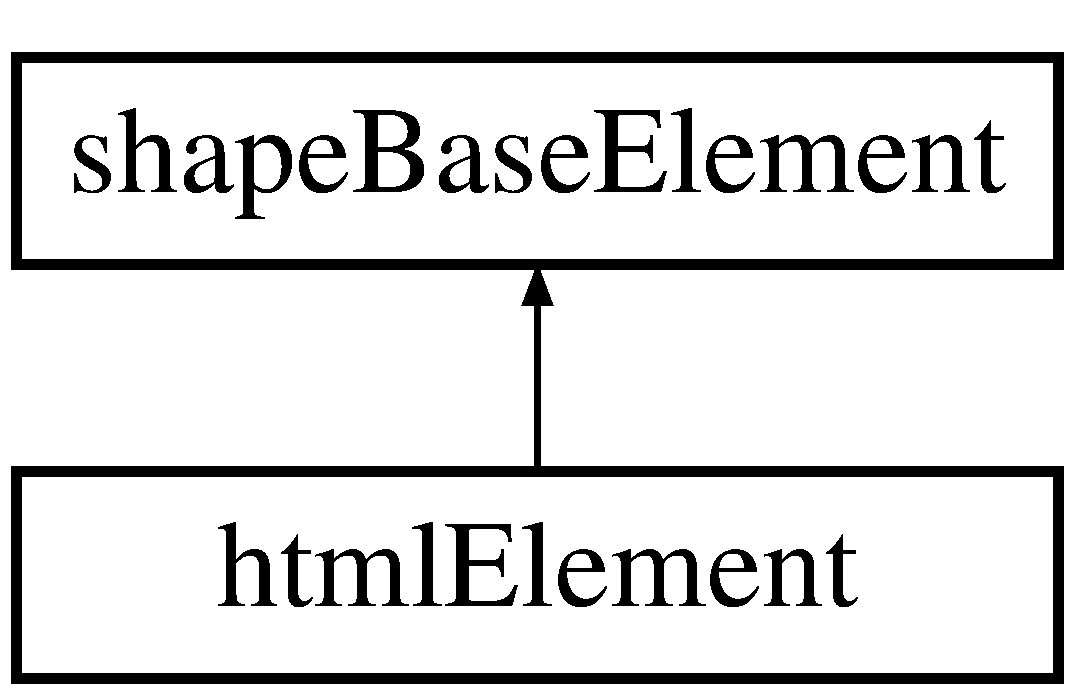
\includegraphics[height=2.000000cm]{classhtmlElement}
\end{center}
\end{figure}
\subsection*{Public Member Functions}
\begin{DoxyCompactItemize}
\item 
\hyperlink{classhtmlElement_a925a2a3ac520421cc180f391922595af}{\+\_\+\+\_\+construct} ()
\item 
\hyperlink{classhtmlElement_ac36b3e96ac37cad8e499b6dd9dad4511}{parse\+Argument} (\$arg)
\item 
\hyperlink{classhtmlElement_a26a8e3284834135dec7b0e01e84b0877}{is\+\_\+assoc} (\$array)
\item 
\hyperlink{classhtmlElement_a1ad02d4640ea217cafe77a53d8b916f0}{\+\_\+\+\_\+to\+String} ()
\item 
\hyperlink{classhtmlElement_ab45087063ba3e42851d01bd87681475b}{compile\+H\+T\+M\+L} ()
\item 
\hyperlink{classhtmlElement_a4e30cd7e3e6d8ad503766d056490c1ef}{compile\+Attributes} ()
\item 
\hyperlink{classhtmlElement_ac05144459b3739d692738dc947f6989c}{compile\+Content} (\$acontent=null)
\item 
\hyperlink{classhtmlElement_af70cbe9883bbe35f9a2573711625cfc4}{template\+H\+T\+M\+L} (\$content, \$\hyperlink{Shape_8php_a774642dc290de09e3aff55c8b594113f}{object})
\item 
\hyperlink{classhtmlElement_aa52ba0af61d736d37927be6894660cd0}{\+\_\+\+\_\+clone} ()
\item 
\hyperlink{classhtmlElement_a89bb434be414cb5e8422141adf272432}{clone\+Children} (\$element)
\item 
\hyperlink{classhtmlElement_ab74714929671cc7cf3271404a621f4ae}{get\+Content} ()
\item 
\hyperlink{classhtmlElement_abf6e0bb5133c6b654e38cb6a78dc91a8}{set\+Content} (\$value)
\item 
\hyperlink{classhtmlElement_ade31cfc5c7d655a21183e18bd0ea492f}{set\+Inherited} ()
\item 
\hyperlink{classhtmlElement_a063bcf0695c98e25ff2b7fa9ef3c88bf}{add\+Content} (\$value)
\item 
\hyperlink{classhtmlElement_a231a77af8cc0ecb36a0714a8888c278f}{by\+Id} (\$key\+Name)
\item 
\hyperlink{classhtmlElement_a8cc57a9db714d6f615bb169424ba505c}{by\+Search} (\$key\+Name, \$key\+Index)
\item 
\hyperlink{classhtmlElement_aae8d6a0e00314fdd72301557161b4054}{by\+Class} (\$key\+Name)
\item 
\hyperlink{classhtmlElement_a329d8c6c7a261b78d39cd4b401320616}{by\+For} (\$key\+Name)
\item 
\hyperlink{classhtmlElement_ac7e4f67382cecd0b2cf4516ef38f0480}{set\+Attribute} (\$key\+Name, \$key\+Value)
\item 
\hyperlink{classhtmlElement_a5e50a939a38f541544c0166871da8853}{clone\+Attribute} (\$attribute)
\item 
\hyperlink{classhtmlElement_a505f41f80a0c7c027dcffe11ee669ff0}{clone\+Content} (\$content)
\item 
\hyperlink{classhtmlElement_a828427f0afb3dc929098581dc7df31b6}{add\+Attribute} (\$key\+Name, \$key\+Value)
\item 
\hyperlink{classhtmlElement_adb7efcd82bb90b24024930604bb9da5d}{set\+Tags} (\$opening\+Tag, \$closing\+Tag, \$compress=\hyperlink{tina4_8php_aec2deb5590a84bee262c3bea206ae88f}{false})
\item 
\hyperlink{classhtmlElement_a60b2acdcaba9e0916863769af9de9b08}{when\+Equal} (\$args)
\item 
\hyperlink{classhtmlElement_afd1361f0a10bdb099102e22f7ecf63d3}{when\+Like} (\$args)
\item 
\hyperlink{classhtmlElement_a93cf423600b179eb6f71e6bcd7a250e2}{when\+Or} (\$args)
\item 
\hyperlink{classhtmlElement_aa6e478845564e185c6f3084196b8e3b8}{when\+And} (\$args)
\item 
\hyperlink{classhtmlElement_abd1779232533ec8dcf26c5154db0c22d}{add\+Data\+Source} (\$name, \$\hyperlink{Shape_8php_a774642dc290de09e3aff55c8b594113f}{object})
\end{DoxyCompactItemize}


\subsection{Detailed Description}
The \hyperlink{classhtmlElement}{html\+Element} class which handles the H\+T\+M\+L compilation etc 

\subsection{Constructor \& Destructor Documentation}
\hypertarget{classhtmlElement_a925a2a3ac520421cc180f391922595af}{}\index{html\+Element@{html\+Element}!\+\_\+\+\_\+construct@{\+\_\+\+\_\+construct}}
\index{\+\_\+\+\_\+construct@{\+\_\+\+\_\+construct}!html\+Element@{html\+Element}}
\subsubsection[{\+\_\+\+\_\+construct}]{\setlength{\rightskip}{0pt plus 5cm}html\+Element\+::\+\_\+\+\_\+construct (
\begin{DoxyParamCaption}
{}
\end{DoxyParamCaption}
)}\label{classhtmlElement_a925a2a3ac520421cc180f391922595af}
Constructor for H\+T\+M\+L\+Element 

\subsection{Member Function Documentation}
\hypertarget{classhtmlElement_aa52ba0af61d736d37927be6894660cd0}{}\index{html\+Element@{html\+Element}!\+\_\+\+\_\+clone@{\+\_\+\+\_\+clone}}
\index{\+\_\+\+\_\+clone@{\+\_\+\+\_\+clone}!html\+Element@{html\+Element}}
\subsubsection[{\+\_\+\+\_\+clone}]{\setlength{\rightskip}{0pt plus 5cm}html\+Element\+::\+\_\+\+\_\+clone (
\begin{DoxyParamCaption}
{}
\end{DoxyParamCaption}
)}\label{classhtmlElement_aa52ba0af61d736d37927be6894660cd0}
Cloning the Object \hypertarget{classhtmlElement_a1ad02d4640ea217cafe77a53d8b916f0}{}\index{html\+Element@{html\+Element}!\+\_\+\+\_\+to\+String@{\+\_\+\+\_\+to\+String}}
\index{\+\_\+\+\_\+to\+String@{\+\_\+\+\_\+to\+String}!html\+Element@{html\+Element}}
\subsubsection[{\+\_\+\+\_\+to\+String}]{\setlength{\rightskip}{0pt plus 5cm}html\+Element\+::\+\_\+\+\_\+to\+String (
\begin{DoxyParamCaption}
{}
\end{DoxyParamCaption}
)}\label{classhtmlElement_a1ad02d4640ea217cafe77a53d8b916f0}
Make H\+T\+M\+L from the Object \begin{DoxyReturn}{Returns}
String H\+T\+M\+L returned from the compile 
\end{DoxyReturn}
\hypertarget{classhtmlElement_a828427f0afb3dc929098581dc7df31b6}{}\index{html\+Element@{html\+Element}!add\+Attribute@{add\+Attribute}}
\index{add\+Attribute@{add\+Attribute}!html\+Element@{html\+Element}}
\subsubsection[{add\+Attribute}]{\setlength{\rightskip}{0pt plus 5cm}html\+Element\+::add\+Attribute (
\begin{DoxyParamCaption}
\item[{}]{\$key\+Name, }
\item[{}]{\$key\+Value}
\end{DoxyParamCaption}
)}\label{classhtmlElement_a828427f0afb3dc929098581dc7df31b6}
Add Attributes to the Element 
\begin{DoxyParams}[1]{Parameters}
type & {\em \$key\+Name} & \\
\hline
type & {\em \$key\+Value} & \\
\hline
\end{DoxyParams}
\hypertarget{classhtmlElement_a063bcf0695c98e25ff2b7fa9ef3c88bf}{}\index{html\+Element@{html\+Element}!add\+Content@{add\+Content}}
\index{add\+Content@{add\+Content}!html\+Element@{html\+Element}}
\subsubsection[{add\+Content}]{\setlength{\rightskip}{0pt plus 5cm}html\+Element\+::add\+Content (
\begin{DoxyParamCaption}
\item[{}]{\$value}
\end{DoxyParamCaption}
)}\label{classhtmlElement_a063bcf0695c98e25ff2b7fa9ef3c88bf}
Adding Content 
\begin{DoxyParams}[1]{Parameters}
type & {\em \$value} & \\
\hline
\end{DoxyParams}
\hypertarget{classhtmlElement_abd1779232533ec8dcf26c5154db0c22d}{}\index{html\+Element@{html\+Element}!add\+Data\+Source@{add\+Data\+Source}}
\index{add\+Data\+Source@{add\+Data\+Source}!html\+Element@{html\+Element}}
\subsubsection[{add\+Data\+Source}]{\setlength{\rightskip}{0pt plus 5cm}html\+Element\+::add\+Data\+Source (
\begin{DoxyParamCaption}
\item[{}]{\$name, }
\item[{}]{\$object}
\end{DoxyParamCaption}
)}\label{classhtmlElement_abd1779232533ec8dcf26c5154db0c22d}
Add a datasource to the shape object for templating 
\begin{DoxyParams}[1]{Parameters}
type & {\em \$object} & \\
\hline
\end{DoxyParams}
\hypertarget{classhtmlElement_aae8d6a0e00314fdd72301557161b4054}{}\index{html\+Element@{html\+Element}!by\+Class@{by\+Class}}
\index{by\+Class@{by\+Class}!html\+Element@{html\+Element}}
\subsubsection[{by\+Class}]{\setlength{\rightskip}{0pt plus 5cm}html\+Element\+::by\+Class (
\begin{DoxyParamCaption}
\item[{}]{\$key\+Name}
\end{DoxyParamCaption}
)}\label{classhtmlElement_aae8d6a0e00314fdd72301557161b4054}
Find and Element by Its H\+T\+M\+L Class Example\+: p(\mbox{[}\char`\"{}clas\char`\"{} =$>$ \char`\"{}\+Test\char`\"{}\mbox{]}) 
\begin{DoxyParams}[1]{Parameters}
type & {\em \$key\+Name} & \\
\hline
\end{DoxyParams}
\begin{DoxyReturn}{Returns}

\end{DoxyReturn}
\hypertarget{classhtmlElement_a329d8c6c7a261b78d39cd4b401320616}{}\index{html\+Element@{html\+Element}!by\+For@{by\+For}}
\index{by\+For@{by\+For}!html\+Element@{html\+Element}}
\subsubsection[{by\+For}]{\setlength{\rightskip}{0pt plus 5cm}html\+Element\+::by\+For (
\begin{DoxyParamCaption}
\item[{}]{\$key\+Name}
\end{DoxyParamCaption}
)}\label{classhtmlElement_a329d8c6c7a261b78d39cd4b401320616}
\hypertarget{classhtmlElement_a231a77af8cc0ecb36a0714a8888c278f}{}\index{html\+Element@{html\+Element}!by\+Id@{by\+Id}}
\index{by\+Id@{by\+Id}!html\+Element@{html\+Element}}
\subsubsection[{by\+Id}]{\setlength{\rightskip}{0pt plus 5cm}html\+Element\+::by\+Id (
\begin{DoxyParamCaption}
\item[{}]{\$key\+Name}
\end{DoxyParamCaption}
)}\label{classhtmlElement_a231a77af8cc0ecb36a0714a8888c278f}
Find and Element by Its H\+T\+M\+L Id Example\+: p(\mbox{[}\char`\"{}id\char`\"{} =$>$ \char`\"{}\+Test\char`\"{}\mbox{]}) 
\begin{DoxyParams}[1]{Parameters}
type & {\em \$key\+Name} & \\
\hline
\end{DoxyParams}
\begin{DoxyReturn}{Returns}

\end{DoxyReturn}
\hypertarget{classhtmlElement_a8cc57a9db714d6f615bb169424ba505c}{}\index{html\+Element@{html\+Element}!by\+Search@{by\+Search}}
\index{by\+Search@{by\+Search}!html\+Element@{html\+Element}}
\subsubsection[{by\+Search}]{\setlength{\rightskip}{0pt plus 5cm}html\+Element\+::by\+Search (
\begin{DoxyParamCaption}
\item[{}]{\$key\+Name, }
\item[{}]{\$key\+Index}
\end{DoxyParamCaption}
)}\label{classhtmlElement_a8cc57a9db714d6f615bb169424ba505c}
By\+Search -\/ internal function to find elements \hypertarget{classhtmlElement_a5e50a939a38f541544c0166871da8853}{}\index{html\+Element@{html\+Element}!clone\+Attribute@{clone\+Attribute}}
\index{clone\+Attribute@{clone\+Attribute}!html\+Element@{html\+Element}}
\subsubsection[{clone\+Attribute}]{\setlength{\rightskip}{0pt plus 5cm}html\+Element\+::clone\+Attribute (
\begin{DoxyParamCaption}
\item[{}]{\$attribute}
\end{DoxyParamCaption}
)}\label{classhtmlElement_a5e50a939a38f541544c0166871da8853}
Clones a new attribute onto the child 
\begin{DoxyParams}[1]{Parameters}
type & {\em \$attribute} & \\
\hline
\end{DoxyParams}
\hypertarget{classhtmlElement_a89bb434be414cb5e8422141adf272432}{}\index{html\+Element@{html\+Element}!clone\+Children@{clone\+Children}}
\index{clone\+Children@{clone\+Children}!html\+Element@{html\+Element}}
\subsubsection[{clone\+Children}]{\setlength{\rightskip}{0pt plus 5cm}html\+Element\+::clone\+Children (
\begin{DoxyParamCaption}
\item[{}]{\$element}
\end{DoxyParamCaption}
)}\label{classhtmlElement_a89bb434be414cb5e8422141adf272432}
Clone All the Children 
\begin{DoxyParams}[1]{Parameters}
type & {\em \$element} & \\
\hline
\end{DoxyParams}
\hypertarget{classhtmlElement_a505f41f80a0c7c027dcffe11ee669ff0}{}\index{html\+Element@{html\+Element}!clone\+Content@{clone\+Content}}
\index{clone\+Content@{clone\+Content}!html\+Element@{html\+Element}}
\subsubsection[{clone\+Content}]{\setlength{\rightskip}{0pt plus 5cm}html\+Element\+::clone\+Content (
\begin{DoxyParamCaption}
\item[{}]{\$content}
\end{DoxyParamCaption}
)}\label{classhtmlElement_a505f41f80a0c7c027dcffe11ee669ff0}
Clones content 
\begin{DoxyParams}[1]{Parameters}
type & {\em \$content} & \\
\hline
\end{DoxyParams}
\hypertarget{classhtmlElement_a4e30cd7e3e6d8ad503766d056490c1ef}{}\index{html\+Element@{html\+Element}!compile\+Attributes@{compile\+Attributes}}
\index{compile\+Attributes@{compile\+Attributes}!html\+Element@{html\+Element}}
\subsubsection[{compile\+Attributes}]{\setlength{\rightskip}{0pt plus 5cm}html\+Element\+::compile\+Attributes (
\begin{DoxyParamCaption}
{}
\end{DoxyParamCaption}
)}\label{classhtmlElement_a4e30cd7e3e6d8ad503766d056490c1ef}
Compile all the Attributes \begin{DoxyReturn}{Returns}
string 
\end{DoxyReturn}
\hypertarget{classhtmlElement_ac05144459b3739d692738dc947f6989c}{}\index{html\+Element@{html\+Element}!compile\+Content@{compile\+Content}}
\index{compile\+Content@{compile\+Content}!html\+Element@{html\+Element}}
\subsubsection[{compile\+Content}]{\setlength{\rightskip}{0pt plus 5cm}html\+Element\+::compile\+Content (
\begin{DoxyParamCaption}
\item[{}]{\$acontent = {\ttfamily null}}
\end{DoxyParamCaption}
)}\label{classhtmlElement_ac05144459b3739d692738dc947f6989c}
Compile the content for the Element 
\begin{DoxyParams}[1]{Parameters}
type & {\em \$acontent} & \\
\hline
\end{DoxyParams}
\begin{DoxyReturn}{Returns}
type 
\end{DoxyReturn}
\hypertarget{classhtmlElement_ab45087063ba3e42851d01bd87681475b}{}\index{html\+Element@{html\+Element}!compile\+H\+T\+M\+L@{compile\+H\+T\+M\+L}}
\index{compile\+H\+T\+M\+L@{compile\+H\+T\+M\+L}!html\+Element@{html\+Element}}
\subsubsection[{compile\+H\+T\+M\+L}]{\setlength{\rightskip}{0pt plus 5cm}html\+Element\+::compile\+H\+T\+M\+L (
\begin{DoxyParamCaption}
{}
\end{DoxyParamCaption}
)}\label{classhtmlElement_ab45087063ba3e42851d01bd87681475b}
Compiling H\+T\+M\+L \begin{DoxyReturn}{Returns}
type 
\end{DoxyReturn}
\hypertarget{classhtmlElement_ab74714929671cc7cf3271404a621f4ae}{}\index{html\+Element@{html\+Element}!get\+Content@{get\+Content}}
\index{get\+Content@{get\+Content}!html\+Element@{html\+Element}}
\subsubsection[{get\+Content}]{\setlength{\rightskip}{0pt plus 5cm}html\+Element\+::get\+Content (
\begin{DoxyParamCaption}
{}
\end{DoxyParamCaption}
)}\label{classhtmlElement_ab74714929671cc7cf3271404a621f4ae}
Getting the content for the Element \begin{DoxyReturn}{Returns}
type 
\end{DoxyReturn}
\hypertarget{classhtmlElement_a26a8e3284834135dec7b0e01e84b0877}{}\index{html\+Element@{html\+Element}!is\+\_\+assoc@{is\+\_\+assoc}}
\index{is\+\_\+assoc@{is\+\_\+assoc}!html\+Element@{html\+Element}}
\subsubsection[{is\+\_\+assoc}]{\setlength{\rightskip}{0pt plus 5cm}html\+Element\+::is\+\_\+assoc (
\begin{DoxyParamCaption}
\item[{}]{\$array}
\end{DoxyParamCaption}
)}\label{classhtmlElement_a26a8e3284834135dec7b0e01e84b0877}
Function to check is an array is an associative or not 
\begin{DoxyParams}[1]{Parameters}
type & {\em \$array} & \\
\hline
\end{DoxyParams}
\begin{DoxyReturn}{Returns}
type 
\end{DoxyReturn}
\hypertarget{classhtmlElement_ac36b3e96ac37cad8e499b6dd9dad4511}{}\index{html\+Element@{html\+Element}!parse\+Argument@{parse\+Argument}}
\index{parse\+Argument@{parse\+Argument}!html\+Element@{html\+Element}}
\subsubsection[{parse\+Argument}]{\setlength{\rightskip}{0pt plus 5cm}html\+Element\+::parse\+Argument (
\begin{DoxyParamCaption}
\item[{}]{\$arg}
\end{DoxyParamCaption}
)}\label{classhtmlElement_ac36b3e96ac37cad8e499b6dd9dad4511}
Parse all the Arguments passed to the class, see if they are content or attributes 
\begin{DoxyParams}[1]{Parameters}
type & {\em \$arg} & \\
\hline
\end{DoxyParams}
\hypertarget{classhtmlElement_ac7e4f67382cecd0b2cf4516ef38f0480}{}\index{html\+Element@{html\+Element}!set\+Attribute@{set\+Attribute}}
\index{set\+Attribute@{set\+Attribute}!html\+Element@{html\+Element}}
\subsubsection[{set\+Attribute}]{\setlength{\rightskip}{0pt plus 5cm}html\+Element\+::set\+Attribute (
\begin{DoxyParamCaption}
\item[{}]{\$key\+Name, }
\item[{}]{\$key\+Value}
\end{DoxyParamCaption}
)}\label{classhtmlElement_ac7e4f67382cecd0b2cf4516ef38f0480}
Set attributes to the Element 
\begin{DoxyParams}[1]{Parameters}
type & {\em \$key\+Name} & \\
\hline
type & {\em \$key\+Value} & \\
\hline
\end{DoxyParams}
\hypertarget{classhtmlElement_abf6e0bb5133c6b654e38cb6a78dc91a8}{}\index{html\+Element@{html\+Element}!set\+Content@{set\+Content}}
\index{set\+Content@{set\+Content}!html\+Element@{html\+Element}}
\subsubsection[{set\+Content}]{\setlength{\rightskip}{0pt plus 5cm}html\+Element\+::set\+Content (
\begin{DoxyParamCaption}
\item[{}]{\$value}
\end{DoxyParamCaption}
)}\label{classhtmlElement_abf6e0bb5133c6b654e38cb6a78dc91a8}
Setting Content 
\begin{DoxyParams}[1]{Parameters}
type & {\em \$value} & \\
\hline
\end{DoxyParams}
\hypertarget{classhtmlElement_ade31cfc5c7d655a21183e18bd0ea492f}{}\index{html\+Element@{html\+Element}!set\+Inherited@{set\+Inherited}}
\index{set\+Inherited@{set\+Inherited}!html\+Element@{html\+Element}}
\subsubsection[{set\+Inherited}]{\setlength{\rightskip}{0pt plus 5cm}html\+Element\+::set\+Inherited (
\begin{DoxyParamCaption}
{}
\end{DoxyParamCaption}
)}\label{classhtmlElement_ade31cfc5c7d655a21183e18bd0ea492f}
Set inherited properties \hypertarget{classhtmlElement_adb7efcd82bb90b24024930604bb9da5d}{}\index{html\+Element@{html\+Element}!set\+Tags@{set\+Tags}}
\index{set\+Tags@{set\+Tags}!html\+Element@{html\+Element}}
\subsubsection[{set\+Tags}]{\setlength{\rightskip}{0pt plus 5cm}html\+Element\+::set\+Tags (
\begin{DoxyParamCaption}
\item[{}]{\$opening\+Tag, }
\item[{}]{\$closing\+Tag, }
\item[{}]{\$compress = {\ttfamily {\bf false}}}
\end{DoxyParamCaption}
)}\label{classhtmlElement_adb7efcd82bb90b24024930604bb9da5d}
Add Opening and Closing Tags 
\begin{DoxyParams}[1]{Parameters}
type & {\em \$opening\+Tag} & \\
\hline
type & {\em \$closing\+Tag} & \\
\hline
\end{DoxyParams}
\hypertarget{classhtmlElement_af70cbe9883bbe35f9a2573711625cfc4}{}\index{html\+Element@{html\+Element}!template\+H\+T\+M\+L@{template\+H\+T\+M\+L}}
\index{template\+H\+T\+M\+L@{template\+H\+T\+M\+L}!html\+Element@{html\+Element}}
\subsubsection[{template\+H\+T\+M\+L}]{\setlength{\rightskip}{0pt plus 5cm}html\+Element\+::template\+H\+T\+M\+L (
\begin{DoxyParamCaption}
\item[{}]{\$content, }
\item[{}]{\$object}
\end{DoxyParamCaption}
)}\label{classhtmlElement_af70cbe9883bbe35f9a2573711625cfc4}
\hypertarget{classhtmlElement_aa6e478845564e185c6f3084196b8e3b8}{}\index{html\+Element@{html\+Element}!when\+And@{when\+And}}
\index{when\+And@{when\+And}!html\+Element@{html\+Element}}
\subsubsection[{when\+And}]{\setlength{\rightskip}{0pt plus 5cm}html\+Element\+::when\+And (
\begin{DoxyParamCaption}
\item[{}]{\$args}
\end{DoxyParamCaption}
)}\label{classhtmlElement_aa6e478845564e185c6f3084196b8e3b8}
Function to evaluate a key value pair for any valid boolean expression, all evaluations should be true 
\begin{DoxyParams}[1]{Parameters}
type & {\em \$args} & \\
\hline
\end{DoxyParams}
\begin{DoxyReturn}{Returns}

\end{DoxyReturn}
\hypertarget{classhtmlElement_a60b2acdcaba9e0916863769af9de9b08}{}\index{html\+Element@{html\+Element}!when\+Equal@{when\+Equal}}
\index{when\+Equal@{when\+Equal}!html\+Element@{html\+Element}}
\subsubsection[{when\+Equal}]{\setlength{\rightskip}{0pt plus 5cm}html\+Element\+::when\+Equal (
\begin{DoxyParamCaption}
\item[{}]{\$args}
\end{DoxyParamCaption}
)}\label{classhtmlElement_a60b2acdcaba9e0916863769af9de9b08}
Function to evaluate a key value pair for a I\+D\+E\+N\+T\+I\+C\+A\+L M\+A\+T\+C\+H -\/ if it is true it returns the current object 
\begin{DoxyParams}[1]{Parameters}
type & {\em \$args} & \\
\hline
\end{DoxyParams}
\begin{DoxyReturn}{Returns}

\end{DoxyReturn}
\hypertarget{classhtmlElement_afd1361f0a10bdb099102e22f7ecf63d3}{}\index{html\+Element@{html\+Element}!when\+Like@{when\+Like}}
\index{when\+Like@{when\+Like}!html\+Element@{html\+Element}}
\subsubsection[{when\+Like}]{\setlength{\rightskip}{0pt plus 5cm}html\+Element\+::when\+Like (
\begin{DoxyParamCaption}
\item[{}]{\$args}
\end{DoxyParamCaption}
)}\label{classhtmlElement_afd1361f0a10bdb099102e22f7ecf63d3}
Function to evaluate a key value pair for a L\+I\+K\+E M\+A\+T\+C\+H -\/ if it is true it returns the current object 
\begin{DoxyParams}[1]{Parameters}
type & {\em \$args} & \\
\hline
\end{DoxyParams}
\begin{DoxyReturn}{Returns}

\end{DoxyReturn}
\hypertarget{classhtmlElement_a93cf423600b179eb6f71e6bcd7a250e2}{}\index{html\+Element@{html\+Element}!when\+Or@{when\+Or}}
\index{when\+Or@{when\+Or}!html\+Element@{html\+Element}}
\subsubsection[{when\+Or}]{\setlength{\rightskip}{0pt plus 5cm}html\+Element\+::when\+Or (
\begin{DoxyParamCaption}
\item[{}]{\$args}
\end{DoxyParamCaption}
)}\label{classhtmlElement_a93cf423600b179eb6f71e6bcd7a250e2}
Function to evaluate a key value pair for any valid boolean expression, all evaluations should be true 
\begin{DoxyParams}[1]{Parameters}
type & {\em \$args} & \\
\hline
\end{DoxyParams}
\begin{DoxyReturn}{Returns}

\end{DoxyReturn}


The documentation for this class was generated from the following file\+:\begin{DoxyCompactItemize}
\item 
web\+\_\+root/tina4/\hyperlink{Shape_8php}{Shape.\+php}\end{DoxyCompactItemize}

\hypertarget{classJSMin}{}\section{J\+S\+Min Class Reference}
\label{classJSMin}\index{J\+S\+Min@{J\+S\+Min}}
\subsection*{Public Member Functions}
\begin{DoxyCompactItemize}
\item 
\hyperlink{classJSMin_a9fcb3a53ccc63a886657053d1609fbf6}{\+\_\+\+\_\+construct} (\$\hyperlink{Shape_8php_a6210da308e7ce036a6362dca3018d6db}{input}=\char`\"{}\char`\"{})
\item 
\hyperlink{classJSMin_a1b73b6860c523a036772bcdf8c99a6ff}{min} ()
\end{DoxyCompactItemize}
\subsection*{Static Public Member Functions}
\begin{DoxyCompactItemize}
\item 
static \hyperlink{classJSMin_a524912007600454e4396aea890384ab6}{minify} (\$js)
\end{DoxyCompactItemize}
\subsection*{Public Attributes}
\begin{DoxyCompactItemize}
\item 
const \hyperlink{classJSMin_ac2104a1ac3a1d438c01c88b7bfafd519}{O\+R\+D\+\_\+\+L\+F} = 10
\item 
const \hyperlink{classJSMin_acae1641c88dbf4928c4a3c5b2428065c}{O\+R\+D\+\_\+\+S\+P\+A\+C\+E} = 32
\item 
const \hyperlink{classJSMin_aadc96fb8e03e7fd45dcc845695db56f6}{A\+C\+T\+I\+O\+N\+\_\+\+K\+E\+E\+P\+\_\+\+A} = 1
\item 
const \hyperlink{classJSMin_a034ff6ce80d8eeffb1548c65b907db73}{A\+C\+T\+I\+O\+N\+\_\+\+D\+E\+L\+E\+T\+E\+\_\+\+A} = 2
\item 
const \hyperlink{classJSMin_a769648a1f5c364c3d964d12d0b4edb8a}{A\+C\+T\+I\+O\+N\+\_\+\+D\+E\+L\+E\+T\+E\+\_\+\+A\+\_\+\+B} = 3
\end{DoxyCompactItemize}
\subsection*{Protected Member Functions}
\begin{DoxyCompactItemize}
\item 
\hyperlink{classJSMin_afecad9e791629529f6b379bd7b20a4e4}{action} (\$command)
\item 
\hyperlink{classJSMin_a487b4b073a8319123317d776feb72f6f}{is\+Regexp\+Literal} ()
\item 
\hyperlink{classJSMin_adcd5b6e8efc1792816812168118f49ef}{get} ()
\item 
\hyperlink{classJSMin_a450a0756edbd9508745f90ccacd08a27}{is\+E\+O\+F} (\$\hyperlink{Shape_8php_a868083704107d6d05b69983f62cce171}{a})
\item 
\hyperlink{classJSMin_ac786ee1b9552762de8fbc7a3a1c22070}{peek} ()
\item 
\hyperlink{classJSMin_af54ff87064c2b9f19e4905e511fc83e5}{is\+Alpha\+Num} (\$c)
\item 
\hyperlink{classJSMin_ad7f3a27d59bdb92db013a336b1c64f3a}{consume\+Single\+Line\+Comment} ()
\item 
\hyperlink{classJSMin_a1bda4db9c558409b8bfc75279a42ca8a}{consume\+Multiple\+Line\+Comment} ()
\item 
\hyperlink{classJSMin_a3c4b356d81d5e5ede03f43cf2aec9037}{next} ()
\end{DoxyCompactItemize}
\subsection*{Protected Attributes}
\begin{DoxyCompactItemize}
\item 
\hyperlink{classJSMin_a2386c0978ac70ac8e9bd592fca835e82}{\$a} = \char`\"{}\textbackslash{}n\char`\"{}
\item 
\hyperlink{classJSMin_aafa0d83dd06ede16a81de0441c5eb1ad}{\$b} = \textquotesingle{}\textquotesingle{}
\item 
\hyperlink{classJSMin_afc2d10997a7e61c31cc9ed70e414829b}{\$input} = \textquotesingle{}\textquotesingle{}
\item 
\hyperlink{classJSMin_a4f772e961c1cd23e3baa6486a2952236}{\$input\+Index} = 0
\item 
\hyperlink{classJSMin_adc61bf642369b9d96e4844b2e694cf76}{\$input\+Length} = 0
\item 
\hyperlink{classJSMin_ad78bd58d8c2f93286068d85abc0afb57}{\$look\+Ahead} = null
\item 
\hyperlink{classJSMin_ab1b9cc7015da8bc3e3cc5edbc60f0ac2}{\$output} = \textquotesingle{}\textquotesingle{}
\item 
\hyperlink{classJSMin_aa33e5c3fabce5f410b11880757bd6521}{\$last\+Byte\+Out} = \textquotesingle{}\textquotesingle{}
\item 
\hyperlink{classJSMin_ac9f663a3d896ddbce3262eae7f777e94}{\$kept\+Comment} = \textquotesingle{}\textquotesingle{}
\end{DoxyCompactItemize}


\subsection{Constructor \& Destructor Documentation}
\hypertarget{classJSMin_a9fcb3a53ccc63a886657053d1609fbf6}{}\index{J\+S\+Min@{J\+S\+Min}!\+\_\+\+\_\+construct@{\+\_\+\+\_\+construct}}
\index{\+\_\+\+\_\+construct@{\+\_\+\+\_\+construct}!J\+S\+Min@{J\+S\+Min}}
\subsubsection[{\+\_\+\+\_\+construct}]{\setlength{\rightskip}{0pt plus 5cm}J\+S\+Min\+::\+\_\+\+\_\+construct (
\begin{DoxyParamCaption}
\item[{}]{\$input = {\ttfamily \char`\"{}\char`\"{}}}
\end{DoxyParamCaption}
)}\label{classJSMin_a9fcb3a53ccc63a886657053d1609fbf6}

\begin{DoxyParams}[1]{Parameters}
string & {\em \$input} & \\
\hline
\end{DoxyParams}


\subsection{Member Function Documentation}
\hypertarget{classJSMin_afecad9e791629529f6b379bd7b20a4e4}{}\index{J\+S\+Min@{J\+S\+Min}!action@{action}}
\index{action@{action}!J\+S\+Min@{J\+S\+Min}}
\subsubsection[{action}]{\setlength{\rightskip}{0pt plus 5cm}J\+S\+Min\+::action (
\begin{DoxyParamCaption}
\item[{}]{\$command}
\end{DoxyParamCaption}
)\hspace{0.3cm}{\ttfamily [protected]}}\label{classJSMin_afecad9e791629529f6b379bd7b20a4e4}
A\+C\+T\+I\+O\+N\+\_\+\+K\+E\+E\+P\+\_\+\+A = Output A. Copy B to A. Get the next B. A\+C\+T\+I\+O\+N\+\_\+\+D\+E\+L\+E\+T\+E\+\_\+\+A = Copy B to A. Get the next B. A\+C\+T\+I\+O\+N\+\_\+\+D\+E\+L\+E\+T\+E\+\_\+\+A\+\_\+\+B = Get the next B.


\begin{DoxyParams}[1]{Parameters}
int & {\em \$command} & \\
\hline
\end{DoxyParams}

\begin{DoxyExceptions}{Exceptions}
{\em J\+S\+Min\+\_\+\+Unterminated\+Reg\+Exp\+Exception$\vert$\+J\+S\+Min\+\_\+\+Unterminated\+String\+Exception} & \\
\hline
\end{DoxyExceptions}
\hypertarget{classJSMin_a1bda4db9c558409b8bfc75279a42ca8a}{}\index{J\+S\+Min@{J\+S\+Min}!consume\+Multiple\+Line\+Comment@{consume\+Multiple\+Line\+Comment}}
\index{consume\+Multiple\+Line\+Comment@{consume\+Multiple\+Line\+Comment}!J\+S\+Min@{J\+S\+Min}}
\subsubsection[{consume\+Multiple\+Line\+Comment}]{\setlength{\rightskip}{0pt plus 5cm}J\+S\+Min\+::consume\+Multiple\+Line\+Comment (
\begin{DoxyParamCaption}
{}
\end{DoxyParamCaption}
)\hspace{0.3cm}{\ttfamily [protected]}}\label{classJSMin_a1bda4db9c558409b8bfc75279a42ca8a}
Consume a multiple line comment from input (possibly retaining it)


\begin{DoxyExceptions}{Exceptions}
{\em \hyperlink{classJSMin__UnterminatedCommentException}{J\+S\+Min\+\_\+\+Unterminated\+Comment\+Exception}} & \\
\hline
\end{DoxyExceptions}
\hypertarget{classJSMin_ad7f3a27d59bdb92db013a336b1c64f3a}{}\index{J\+S\+Min@{J\+S\+Min}!consume\+Single\+Line\+Comment@{consume\+Single\+Line\+Comment}}
\index{consume\+Single\+Line\+Comment@{consume\+Single\+Line\+Comment}!J\+S\+Min@{J\+S\+Min}}
\subsubsection[{consume\+Single\+Line\+Comment}]{\setlength{\rightskip}{0pt plus 5cm}J\+S\+Min\+::consume\+Single\+Line\+Comment (
\begin{DoxyParamCaption}
{}
\end{DoxyParamCaption}
)\hspace{0.3cm}{\ttfamily [protected]}}\label{classJSMin_ad7f3a27d59bdb92db013a336b1c64f3a}
Consume a single line comment from input (possibly retaining it) \hypertarget{classJSMin_adcd5b6e8efc1792816812168118f49ef}{}\index{J\+S\+Min@{J\+S\+Min}!get@{get}}
\index{get@{get}!J\+S\+Min@{J\+S\+Min}}
\subsubsection[{get}]{\setlength{\rightskip}{0pt plus 5cm}J\+S\+Min\+::get (
\begin{DoxyParamCaption}
{}
\end{DoxyParamCaption}
)\hspace{0.3cm}{\ttfamily [protected]}}\label{classJSMin_adcd5b6e8efc1792816812168118f49ef}
Return the next character from stdin. Watch out for lookahead. If the character is a control character, translate it to a space or linefeed.

\begin{DoxyReturn}{Returns}
string 
\end{DoxyReturn}
\hypertarget{classJSMin_af54ff87064c2b9f19e4905e511fc83e5}{}\index{J\+S\+Min@{J\+S\+Min}!is\+Alpha\+Num@{is\+Alpha\+Num}}
\index{is\+Alpha\+Num@{is\+Alpha\+Num}!J\+S\+Min@{J\+S\+Min}}
\subsubsection[{is\+Alpha\+Num}]{\setlength{\rightskip}{0pt plus 5cm}J\+S\+Min\+::is\+Alpha\+Num (
\begin{DoxyParamCaption}
\item[{}]{\$c}
\end{DoxyParamCaption}
)\hspace{0.3cm}{\ttfamily [protected]}}\label{classJSMin_af54ff87064c2b9f19e4905e511fc83e5}
Return true if the character is a letter, digit, underscore, dollar sign, or non-\/\+A\+S\+C\+I\+I character.


\begin{DoxyParams}[1]{Parameters}
string & {\em \$c} & \\
\hline
\end{DoxyParams}
\begin{DoxyReturn}{Returns}
bool 
\end{DoxyReturn}
\hypertarget{classJSMin_a450a0756edbd9508745f90ccacd08a27}{}\index{J\+S\+Min@{J\+S\+Min}!is\+E\+O\+F@{is\+E\+O\+F}}
\index{is\+E\+O\+F@{is\+E\+O\+F}!J\+S\+Min@{J\+S\+Min}}
\subsubsection[{is\+E\+O\+F}]{\setlength{\rightskip}{0pt plus 5cm}J\+S\+Min\+::is\+E\+O\+F (
\begin{DoxyParamCaption}
\item[{}]{\$a}
\end{DoxyParamCaption}
)\hspace{0.3cm}{\ttfamily [protected]}}\label{classJSMin_a450a0756edbd9508745f90ccacd08a27}
Does \$a indicate end of input?


\begin{DoxyParams}[1]{Parameters}
string & {\em \$a} & \\
\hline
\end{DoxyParams}
\begin{DoxyReturn}{Returns}
bool 
\end{DoxyReturn}
\hypertarget{classJSMin_a487b4b073a8319123317d776feb72f6f}{}\index{J\+S\+Min@{J\+S\+Min}!is\+Regexp\+Literal@{is\+Regexp\+Literal}}
\index{is\+Regexp\+Literal@{is\+Regexp\+Literal}!J\+S\+Min@{J\+S\+Min}}
\subsubsection[{is\+Regexp\+Literal}]{\setlength{\rightskip}{0pt plus 5cm}J\+S\+Min\+::is\+Regexp\+Literal (
\begin{DoxyParamCaption}
{}
\end{DoxyParamCaption}
)\hspace{0.3cm}{\ttfamily [protected]}}\label{classJSMin_a487b4b073a8319123317d776feb72f6f}
\begin{DoxyReturn}{Returns}
bool 
\end{DoxyReturn}
\hypertarget{classJSMin_a1b73b6860c523a036772bcdf8c99a6ff}{}\index{J\+S\+Min@{J\+S\+Min}!min@{min}}
\index{min@{min}!J\+S\+Min@{J\+S\+Min}}
\subsubsection[{min}]{\setlength{\rightskip}{0pt plus 5cm}J\+S\+Min\+::min (
\begin{DoxyParamCaption}
{}
\end{DoxyParamCaption}
)}\label{classJSMin_a1b73b6860c523a036772bcdf8c99a6ff}
Perform minification, return result

\begin{DoxyReturn}{Returns}
string 
\end{DoxyReturn}
\hypertarget{classJSMin_a524912007600454e4396aea890384ab6}{}\index{J\+S\+Min@{J\+S\+Min}!minify@{minify}}
\index{minify@{minify}!J\+S\+Min@{J\+S\+Min}}
\subsubsection[{minify}]{\setlength{\rightskip}{0pt plus 5cm}static J\+S\+Min\+::minify (
\begin{DoxyParamCaption}
\item[{}]{\$js}
\end{DoxyParamCaption}
)\hspace{0.3cm}{\ttfamily [static]}}\label{classJSMin_a524912007600454e4396aea890384ab6}
Minify Javascript.


\begin{DoxyParams}[1]{Parameters}
string & {\em \$js} & Javascript to be minified\\
\hline
\end{DoxyParams}
\begin{DoxyReturn}{Returns}
string 
\end{DoxyReturn}
\hypertarget{classJSMin_a3c4b356d81d5e5ede03f43cf2aec9037}{}\index{J\+S\+Min@{J\+S\+Min}!next@{next}}
\index{next@{next}!J\+S\+Min@{J\+S\+Min}}
\subsubsection[{next}]{\setlength{\rightskip}{0pt plus 5cm}J\+S\+Min\+::next (
\begin{DoxyParamCaption}
{}
\end{DoxyParamCaption}
)\hspace{0.3cm}{\ttfamily [protected]}}\label{classJSMin_a3c4b356d81d5e5ede03f43cf2aec9037}
Get the next character, skipping over comments. Some comments may be preserved.

\begin{DoxyReturn}{Returns}
string 
\end{DoxyReturn}
\hypertarget{classJSMin_ac786ee1b9552762de8fbc7a3a1c22070}{}\index{J\+S\+Min@{J\+S\+Min}!peek@{peek}}
\index{peek@{peek}!J\+S\+Min@{J\+S\+Min}}
\subsubsection[{peek}]{\setlength{\rightskip}{0pt plus 5cm}J\+S\+Min\+::peek (
\begin{DoxyParamCaption}
{}
\end{DoxyParamCaption}
)\hspace{0.3cm}{\ttfamily [protected]}}\label{classJSMin_ac786ee1b9552762de8fbc7a3a1c22070}
Get next char (without getting it). If is ctrl character, translate to a space or newline.

\begin{DoxyReturn}{Returns}
string 
\end{DoxyReturn}


\subsection{Member Data Documentation}
\hypertarget{classJSMin_a2386c0978ac70ac8e9bd592fca835e82}{}\index{J\+S\+Min@{J\+S\+Min}!\$a@{\$a}}
\index{\$a@{\$a}!J\+S\+Min@{J\+S\+Min}}
\subsubsection[{\$a}]{\setlength{\rightskip}{0pt plus 5cm}J\+S\+Min\+::\$a = \char`\"{}\textbackslash{}n\char`\"{}\hspace{0.3cm}{\ttfamily [protected]}}\label{classJSMin_a2386c0978ac70ac8e9bd592fca835e82}
\hypertarget{classJSMin_aafa0d83dd06ede16a81de0441c5eb1ad}{}\index{J\+S\+Min@{J\+S\+Min}!\$b@{\$b}}
\index{\$b@{\$b}!J\+S\+Min@{J\+S\+Min}}
\subsubsection[{\$b}]{\setlength{\rightskip}{0pt plus 5cm}J\+S\+Min\+::\$b = \textquotesingle{}\textquotesingle{}\hspace{0.3cm}{\ttfamily [protected]}}\label{classJSMin_aafa0d83dd06ede16a81de0441c5eb1ad}
\hypertarget{classJSMin_afc2d10997a7e61c31cc9ed70e414829b}{}\index{J\+S\+Min@{J\+S\+Min}!\$input@{\$input}}
\index{\$input@{\$input}!J\+S\+Min@{J\+S\+Min}}
\subsubsection[{\$input}]{\setlength{\rightskip}{0pt plus 5cm}J\+S\+Min\+::\$input = \textquotesingle{}\textquotesingle{}\hspace{0.3cm}{\ttfamily [protected]}}\label{classJSMin_afc2d10997a7e61c31cc9ed70e414829b}
\hypertarget{classJSMin_a4f772e961c1cd23e3baa6486a2952236}{}\index{J\+S\+Min@{J\+S\+Min}!\$input\+Index@{\$input\+Index}}
\index{\$input\+Index@{\$input\+Index}!J\+S\+Min@{J\+S\+Min}}
\subsubsection[{\$input\+Index}]{\setlength{\rightskip}{0pt plus 5cm}J\+S\+Min\+::\$input\+Index = 0\hspace{0.3cm}{\ttfamily [protected]}}\label{classJSMin_a4f772e961c1cd23e3baa6486a2952236}
\hypertarget{classJSMin_adc61bf642369b9d96e4844b2e694cf76}{}\index{J\+S\+Min@{J\+S\+Min}!\$input\+Length@{\$input\+Length}}
\index{\$input\+Length@{\$input\+Length}!J\+S\+Min@{J\+S\+Min}}
\subsubsection[{\$input\+Length}]{\setlength{\rightskip}{0pt plus 5cm}J\+S\+Min\+::\$input\+Length = 0\hspace{0.3cm}{\ttfamily [protected]}}\label{classJSMin_adc61bf642369b9d96e4844b2e694cf76}
\hypertarget{classJSMin_ac9f663a3d896ddbce3262eae7f777e94}{}\index{J\+S\+Min@{J\+S\+Min}!\$kept\+Comment@{\$kept\+Comment}}
\index{\$kept\+Comment@{\$kept\+Comment}!J\+S\+Min@{J\+S\+Min}}
\subsubsection[{\$kept\+Comment}]{\setlength{\rightskip}{0pt plus 5cm}J\+S\+Min\+::\$kept\+Comment = \textquotesingle{}\textquotesingle{}\hspace{0.3cm}{\ttfamily [protected]}}\label{classJSMin_ac9f663a3d896ddbce3262eae7f777e94}
\hypertarget{classJSMin_aa33e5c3fabce5f410b11880757bd6521}{}\index{J\+S\+Min@{J\+S\+Min}!\$last\+Byte\+Out@{\$last\+Byte\+Out}}
\index{\$last\+Byte\+Out@{\$last\+Byte\+Out}!J\+S\+Min@{J\+S\+Min}}
\subsubsection[{\$last\+Byte\+Out}]{\setlength{\rightskip}{0pt plus 5cm}J\+S\+Min\+::\$last\+Byte\+Out = \textquotesingle{}\textquotesingle{}\hspace{0.3cm}{\ttfamily [protected]}}\label{classJSMin_aa33e5c3fabce5f410b11880757bd6521}
\hypertarget{classJSMin_ad78bd58d8c2f93286068d85abc0afb57}{}\index{J\+S\+Min@{J\+S\+Min}!\$look\+Ahead@{\$look\+Ahead}}
\index{\$look\+Ahead@{\$look\+Ahead}!J\+S\+Min@{J\+S\+Min}}
\subsubsection[{\$look\+Ahead}]{\setlength{\rightskip}{0pt plus 5cm}J\+S\+Min\+::\$look\+Ahead = null\hspace{0.3cm}{\ttfamily [protected]}}\label{classJSMin_ad78bd58d8c2f93286068d85abc0afb57}
\hypertarget{classJSMin_ab1b9cc7015da8bc3e3cc5edbc60f0ac2}{}\index{J\+S\+Min@{J\+S\+Min}!\$output@{\$output}}
\index{\$output@{\$output}!J\+S\+Min@{J\+S\+Min}}
\subsubsection[{\$output}]{\setlength{\rightskip}{0pt plus 5cm}J\+S\+Min\+::\$output = \textquotesingle{}\textquotesingle{}\hspace{0.3cm}{\ttfamily [protected]}}\label{classJSMin_ab1b9cc7015da8bc3e3cc5edbc60f0ac2}
\hypertarget{classJSMin_a034ff6ce80d8eeffb1548c65b907db73}{}\index{J\+S\+Min@{J\+S\+Min}!A\+C\+T\+I\+O\+N\+\_\+\+D\+E\+L\+E\+T\+E\+\_\+\+A@{A\+C\+T\+I\+O\+N\+\_\+\+D\+E\+L\+E\+T\+E\+\_\+\+A}}
\index{A\+C\+T\+I\+O\+N\+\_\+\+D\+E\+L\+E\+T\+E\+\_\+\+A@{A\+C\+T\+I\+O\+N\+\_\+\+D\+E\+L\+E\+T\+E\+\_\+\+A}!J\+S\+Min@{J\+S\+Min}}
\subsubsection[{A\+C\+T\+I\+O\+N\+\_\+\+D\+E\+L\+E\+T\+E\+\_\+\+A}]{\setlength{\rightskip}{0pt plus 5cm}const J\+S\+Min\+::\+A\+C\+T\+I\+O\+N\+\_\+\+D\+E\+L\+E\+T\+E\+\_\+\+A = 2}\label{classJSMin_a034ff6ce80d8eeffb1548c65b907db73}
\hypertarget{classJSMin_a769648a1f5c364c3d964d12d0b4edb8a}{}\index{J\+S\+Min@{J\+S\+Min}!A\+C\+T\+I\+O\+N\+\_\+\+D\+E\+L\+E\+T\+E\+\_\+\+A\+\_\+\+B@{A\+C\+T\+I\+O\+N\+\_\+\+D\+E\+L\+E\+T\+E\+\_\+\+A\+\_\+\+B}}
\index{A\+C\+T\+I\+O\+N\+\_\+\+D\+E\+L\+E\+T\+E\+\_\+\+A\+\_\+\+B@{A\+C\+T\+I\+O\+N\+\_\+\+D\+E\+L\+E\+T\+E\+\_\+\+A\+\_\+\+B}!J\+S\+Min@{J\+S\+Min}}
\subsubsection[{A\+C\+T\+I\+O\+N\+\_\+\+D\+E\+L\+E\+T\+E\+\_\+\+A\+\_\+\+B}]{\setlength{\rightskip}{0pt plus 5cm}const J\+S\+Min\+::\+A\+C\+T\+I\+O\+N\+\_\+\+D\+E\+L\+E\+T\+E\+\_\+\+A\+\_\+\+B = 3}\label{classJSMin_a769648a1f5c364c3d964d12d0b4edb8a}
\hypertarget{classJSMin_aadc96fb8e03e7fd45dcc845695db56f6}{}\index{J\+S\+Min@{J\+S\+Min}!A\+C\+T\+I\+O\+N\+\_\+\+K\+E\+E\+P\+\_\+\+A@{A\+C\+T\+I\+O\+N\+\_\+\+K\+E\+E\+P\+\_\+\+A}}
\index{A\+C\+T\+I\+O\+N\+\_\+\+K\+E\+E\+P\+\_\+\+A@{A\+C\+T\+I\+O\+N\+\_\+\+K\+E\+E\+P\+\_\+\+A}!J\+S\+Min@{J\+S\+Min}}
\subsubsection[{A\+C\+T\+I\+O\+N\+\_\+\+K\+E\+E\+P\+\_\+\+A}]{\setlength{\rightskip}{0pt plus 5cm}const J\+S\+Min\+::\+A\+C\+T\+I\+O\+N\+\_\+\+K\+E\+E\+P\+\_\+\+A = 1}\label{classJSMin_aadc96fb8e03e7fd45dcc845695db56f6}
\hypertarget{classJSMin_ac2104a1ac3a1d438c01c88b7bfafd519}{}\index{J\+S\+Min@{J\+S\+Min}!O\+R\+D\+\_\+\+L\+F@{O\+R\+D\+\_\+\+L\+F}}
\index{O\+R\+D\+\_\+\+L\+F@{O\+R\+D\+\_\+\+L\+F}!J\+S\+Min@{J\+S\+Min}}
\subsubsection[{O\+R\+D\+\_\+\+L\+F}]{\setlength{\rightskip}{0pt plus 5cm}const J\+S\+Min\+::\+O\+R\+D\+\_\+\+L\+F = 10}\label{classJSMin_ac2104a1ac3a1d438c01c88b7bfafd519}
\hypertarget{classJSMin_acae1641c88dbf4928c4a3c5b2428065c}{}\index{J\+S\+Min@{J\+S\+Min}!O\+R\+D\+\_\+\+S\+P\+A\+C\+E@{O\+R\+D\+\_\+\+S\+P\+A\+C\+E}}
\index{O\+R\+D\+\_\+\+S\+P\+A\+C\+E@{O\+R\+D\+\_\+\+S\+P\+A\+C\+E}!J\+S\+Min@{J\+S\+Min}}
\subsubsection[{O\+R\+D\+\_\+\+S\+P\+A\+C\+E}]{\setlength{\rightskip}{0pt plus 5cm}const J\+S\+Min\+::\+O\+R\+D\+\_\+\+S\+P\+A\+C\+E = 32}\label{classJSMin_acae1641c88dbf4928c4a3c5b2428065c}


The documentation for this class was generated from the following file\+:\begin{DoxyCompactItemize}
\item 
web\+\_\+root/tina4/\hyperlink{Shape_8php}{Shape.\+php}\end{DoxyCompactItemize}

\hypertarget{classJSMin__UnterminatedCommentException}{}\section{J\+S\+Min\+\_\+\+Unterminated\+Comment\+Exception Class Reference}
\label{classJSMin__UnterminatedCommentException}\index{J\+S\+Min\+\_\+\+Unterminated\+Comment\+Exception@{J\+S\+Min\+\_\+\+Unterminated\+Comment\+Exception}}
Inheritance diagram for J\+S\+Min\+\_\+\+Unterminated\+Comment\+Exception\+:\begin{figure}[H]
\begin{center}
\leavevmode
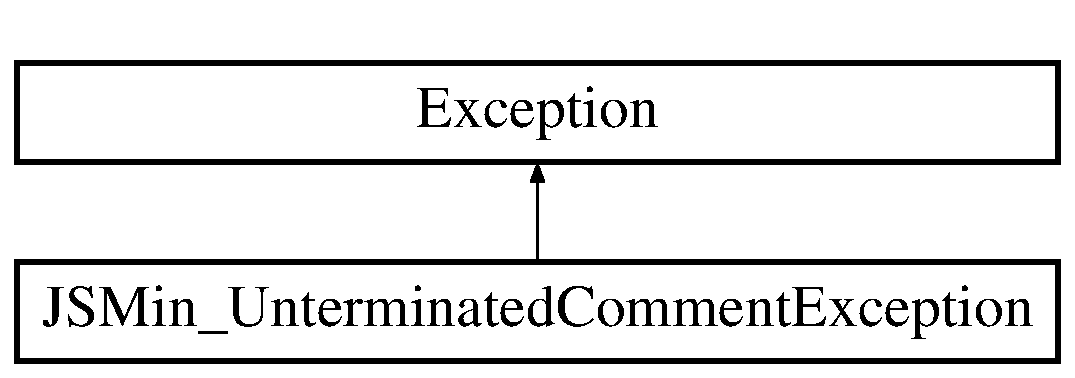
\includegraphics[height=2.000000cm]{classJSMin__UnterminatedCommentException}
\end{center}
\end{figure}


The documentation for this class was generated from the following file\+:\begin{DoxyCompactItemize}
\item 
web\+\_\+root/tina4/\hyperlink{Shape_8php}{Shape.\+php}\end{DoxyCompactItemize}

\hypertarget{classJSMin__UnterminatedRegExpException}{}\section{J\+S\+Min\+\_\+\+Unterminated\+Reg\+Exp\+Exception Class Reference}
\label{classJSMin__UnterminatedRegExpException}\index{J\+S\+Min\+\_\+\+Unterminated\+Reg\+Exp\+Exception@{J\+S\+Min\+\_\+\+Unterminated\+Reg\+Exp\+Exception}}
Inheritance diagram for J\+S\+Min\+\_\+\+Unterminated\+Reg\+Exp\+Exception\+:\begin{figure}[H]
\begin{center}
\leavevmode
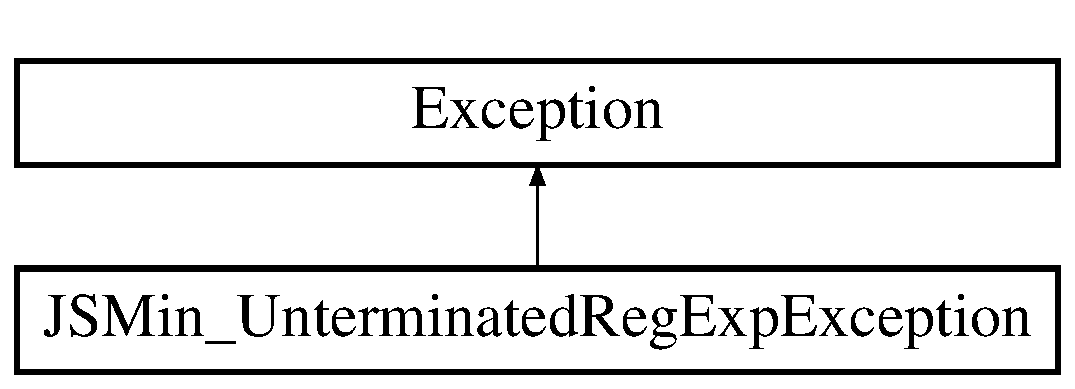
\includegraphics[height=2.000000cm]{classJSMin__UnterminatedRegExpException}
\end{center}
\end{figure}


The documentation for this class was generated from the following file\+:\begin{DoxyCompactItemize}
\item 
web\+\_\+root/tina4/\hyperlink{Shape_8php}{Shape.\+php}\end{DoxyCompactItemize}

\hypertarget{classJSMin__UnterminatedStringException}{}\section{J\+S\+Min\+\_\+\+Unterminated\+String\+Exception Class Reference}
\label{classJSMin__UnterminatedStringException}\index{J\+S\+Min\+\_\+\+Unterminated\+String\+Exception@{J\+S\+Min\+\_\+\+Unterminated\+String\+Exception}}
Inheritance diagram for J\+S\+Min\+\_\+\+Unterminated\+String\+Exception\+:\begin{figure}[H]
\begin{center}
\leavevmode
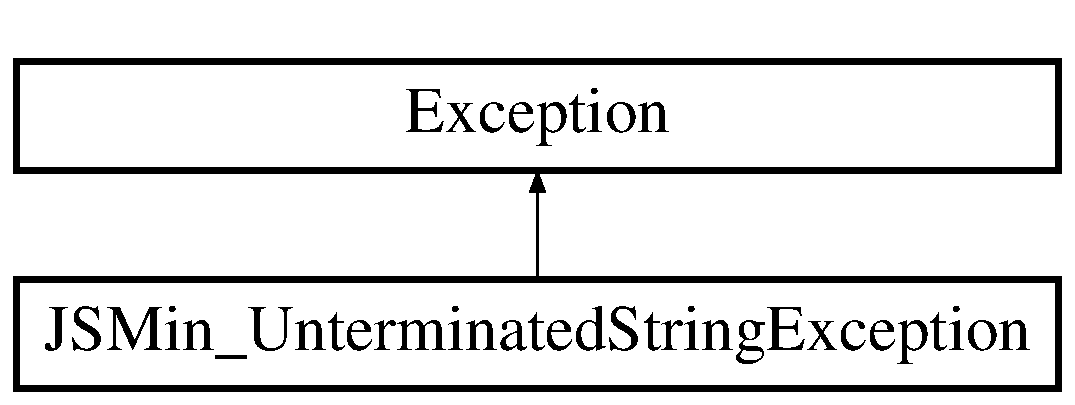
\includegraphics[height=2.000000cm]{classJSMin__UnterminatedStringException}
\end{center}
\end{figure}


The documentation for this class was generated from the following file\+:\begin{DoxyCompactItemize}
\item 
web\+\_\+root/tina4/\hyperlink{Shape_8php}{Shape.\+php}\end{DoxyCompactItemize}

\hypertarget{classKim}{}\section{Kim Class Reference}
\label{classKim}\index{Kim@{Kim}}
\subsection*{Public Member Functions}
\begin{DoxyCompactItemize}
\item 
\hyperlink{classKim_a23fe2ba2b5a76fe09200e2f0fbded794}{\+\_\+\+\_\+construct} ()
\item 
\hyperlink{classKim_a98cd6f87644136345cd5203952f4ddbb}{link\+Array} (\$m)
\item 
\hyperlink{classKim_a8a754c69958e71d159e6808f83f12cfe}{get\+Default\+Page} (\$page\+Name)
\item 
\hyperlink{classKim_ae9db930151f99235866c68fd96208cd8}{create\+Database} ()
\item 
\hyperlink{classKim_adbe9f842961805e68a08df04c4c58dfd}{get\+Call\+Params} (\$\hyperlink{Shape_8php_a6210da308e7ce036a6362dca3018d6db}{input})
\item 
\hyperlink{classKim_a960a80702fe7dd134adbfeea34ccfcfa}{parse\+Snippets} (\$elements, \$template, \$data)
\item 
\hyperlink{classKim_ae484524c4622734ede53894ae89a669a}{get\+Template} (\$template, \$data=\char`\"{}\char`\"{})
\item 
\hyperlink{classKim_a635cc5c4509bd3ac1c578ccfe62c623b}{parse\+Template} (\$template, \$data=\char`\"{}\char`\"{})
\item 
\hyperlink{classKim_a3cb9fd00227b180b8118257b85acf6ff}{get\+Page\+Template} (\$\hyperlink{Shape_8php_ad264ad0cabbe965bf7f7c8a5ed6abebb}{title}=\char`\"{}Default\char`\"{})
\item 
\hyperlink{classKim_a76d369e52b95a9cabdb45c793d3eee45}{get\+Sub\+Menus} (\$menu\+Id=0, \$system\+Menu=1)
\item 
\hyperlink{classKim_ad7f2c106626bd9e83f1a4f76303a6e45}{get\+Menu\+List} (\$parent\+Id=0, \$system\+Menu=1)
\item 
\hyperlink{classKim_ac4c6f020c4abed55574cc4515b8c1b01}{get\+Menu} (\$parent\+Id=0, \$system\+Menu=1)
\item 
\hyperlink{classKim_a7391f7a7d90adef0a048f2679aaa27fd}{get\+Insert\+Menu\+Item\+Form} ()
\item 
\hyperlink{classKim_a03aa4a733e4539d175df84011ad1cb9a}{insert\+Menu\+Item} ()
\item 
\hyperlink{classKim_ab0a2f80e33b3d6ed654fbf6b8cf55291}{delete\+Menu\+Item} ()
\item 
\hyperlink{classKim_a1c8f6358dbec4612dd880ae09cb4a74e}{update\+Menu\+Item} ()
\item 
\hyperlink{classKim_a2a73684a878eac950d34f15ce674f194}{get\+Menu\+Item\+Form} (\$menu\+Id)
\item 
\hyperlink{classKim_a7f493912f2db5510a30faebd9b553162}{get\+Menu\+Tree} (\$filter=\char`\"{}where system\+\_\+menu $<$$>$ 1 and parent\+\_\+id = 0\char`\"{}, \$menu\+Id=0)
\item 
\hyperlink{classKim_afce7f678a883aab27b976429e8248d79}{get\+User\+List} (\$filter=\char`\"{}\char`\"{})
\item 
\hyperlink{classKim_a0fb70ab1aedbf3be92bfdd9241944e6b}{get\+Menu\+Creator} ()
\item 
\hyperlink{classKim_a31a5796278c813534e76d2ce91d9eed2}{get\+Users} ()
\item 
\hyperlink{classKim_a03d8b762e1c6d458e714904cd8b02dd6}{get\+User\+Types} ()
\item 
\hyperlink{classKim_a8ed17935db3df4dfc01b2b26d47ebc4e}{get\+Route\+Target} (\$record\+Value=null)
\item 
\hyperlink{classKim_a1e3ce6c13bf4c0b488ff07ddfe95c0ac}{get\+Routes} ()
\item 
\hyperlink{classKim_a5fcd3a64ecd0f244e9db70f0c007b6ba}{cache\+Routes} ()
\item 
\hyperlink{classKim_a99011f068ed5a1f55fd8c5cf2b1aac43}{load\+Routes} ()
\item 
\hyperlink{classKim_a2bcf75443f82b5c8f49b4e82bdcab94d}{get\+Global\+Settings} ()
\item 
\hyperlink{classKim_a54e4f46e005a09de5bda3a2093a86af7}{get\+Flush\+X\+Cache} ()
\item 
\hyperlink{classKim_a7531e4d2f4da4cb34176d40d20ee6401}{get\+Login} ()
\item 
\hyperlink{classKim_abfaef7d8d59b67ed50d46053b0154b1d}{authenticate} ()
\item 
\hyperlink{classKim_a6c3ce83f2f3bc3c7743f1bfa46f30d0e}{get\+User\+Record} (\$user\+Id=0)
\item 
\hyperlink{classKim_acbae7ab945d82706b2be25816578ae71}{get\+Profile\+Update} ()
\item 
\hyperlink{classKim_a3725ce24c9501992a03e6386423e447c}{update\+P\+O\+S\+T} ()
\item 
\hyperlink{classKim_a1187d9c11984f0daf1f6fa983378d4e7}{clean\+Up\+Conditions} (\$\hyperlink{Shape_8php_a868083704107d6d05b69983f62cce171}{a})
\item 
\hyperlink{classKim_a06415955f55535b121470e7779e92168}{match\+Conditions} (\$string)
\item 
\hyperlink{classKim_ae017a30aaa5b1f6e470de679142b7f02}{display} ()
\end{DoxyCompactItemize}
\subsection*{Public Attributes}
\begin{DoxyCompactItemize}
\item 
\hyperlink{classKim_a68fb575a2ef7faf6b3b679280331033d}{\$create\+D\+B}
\item 
\hyperlink{classKim_a46554f1a34a5f3db1014d47b6ec37f00}{\$\+K\+I\+M}
\item 
\hyperlink{classKim_a761d5be4968e338c3d7ffa9f65ae3a40}{\$default\+Pages} = \mbox{[}\char`\"{}index.\+html\char`\"{}, \char`\"{}index.\+php\char`\"{}, \char`\"{}\hyperlink{Shape_8php_a8b267aa0adca2018097f6f6f4c804d46}{home.\+html}\char`\"{}\mbox{]}
\item 
\hyperlink{classKim_aecfd2bbe4c11ceb39810c393cd357b53}{\$default\+Extensions} = \mbox{[}\char`\"{}.html\char`\"{}, \char`\"{}.php\char`\"{}\mbox{]}
\end{DoxyCompactItemize}


\subsection{Detailed Description}
\hyperlink{classKim}{Kim} is a class to handle the menu driven roles and routes for Tina4 \hyperlink{}{http\+://localhost\+:12345/dokuwiki/kim}

\subsection{Constructor \& Destructor Documentation}
\hypertarget{classKim_a23fe2ba2b5a76fe09200e2f0fbded794}{}\index{Kim@{Kim}!\+\_\+\+\_\+construct@{\+\_\+\+\_\+construct}}
\index{\+\_\+\+\_\+construct@{\+\_\+\+\_\+construct}!Kim@{Kim}}
\subsubsection[{\+\_\+\+\_\+construct}]{\setlength{\rightskip}{0pt plus 5cm}Kim\+::\+\_\+\+\_\+construct (
\begin{DoxyParamCaption}
{}
\end{DoxyParamCaption}
)}\label{classKim_a23fe2ba2b5a76fe09200e2f0fbded794}
Create a database connection for \hyperlink{classKim}{Kim} to use. Check if we need to be creating the database for the menus

\subsection{Member Function Documentation}
\hypertarget{classKim_abfaef7d8d59b67ed50d46053b0154b1d}{}\index{Kim@{Kim}!authenticate@{authenticate}}
\index{authenticate@{authenticate}!Kim@{Kim}}
\subsubsection[{authenticate}]{\setlength{\rightskip}{0pt plus 5cm}Kim\+::authenticate (
\begin{DoxyParamCaption}
{}
\end{DoxyParamCaption}
)}\label{classKim_abfaef7d8d59b67ed50d46053b0154b1d}
\hypertarget{classKim_a5fcd3a64ecd0f244e9db70f0c007b6ba}{}\index{Kim@{Kim}!cache\+Routes@{cache\+Routes}}
\index{cache\+Routes@{cache\+Routes}!Kim@{Kim}}
\subsubsection[{cache\+Routes}]{\setlength{\rightskip}{0pt plus 5cm}Kim\+::cache\+Routes (
\begin{DoxyParamCaption}
{}
\end{DoxyParamCaption}
)}\label{classKim_a5fcd3a64ecd0f244e9db70f0c007b6ba}
\hypertarget{classKim_a1187d9c11984f0daf1f6fa983378d4e7}{}\index{Kim@{Kim}!clean\+Up\+Conditions@{clean\+Up\+Conditions}}
\index{clean\+Up\+Conditions@{clean\+Up\+Conditions}!Kim@{Kim}}
\subsubsection[{clean\+Up\+Conditions}]{\setlength{\rightskip}{0pt plus 5cm}Kim\+::clean\+Up\+Conditions (
\begin{DoxyParamCaption}
\item[{}]{\$a}
\end{DoxyParamCaption}
)}\label{classKim_a1187d9c11984f0daf1f6fa983378d4e7}
Cleans up the input String of a Condition 
\begin{DoxyParams}[1]{Parameters}
type & {\em \$input\+String} & \\
\hline
\end{DoxyParams}
\begin{DoxyReturn}{Returns}
type 
\end{DoxyReturn}
\hypertarget{classKim_ae9db930151f99235866c68fd96208cd8}{}\index{Kim@{Kim}!create\+Database@{create\+Database}}
\index{create\+Database@{create\+Database}!Kim@{Kim}}
\subsubsection[{create\+Database}]{\setlength{\rightskip}{0pt plus 5cm}Kim\+::create\+Database (
\begin{DoxyParamCaption}
{}
\end{DoxyParamCaption}
)}\label{classKim_ae9db930151f99235866c68fd96208cd8}
Function to create the tables for \hyperlink{classKim}{Kim} to be used with roles, routes, menus \hypertarget{classKim_ab0a2f80e33b3d6ed654fbf6b8cf55291}{}\index{Kim@{Kim}!delete\+Menu\+Item@{delete\+Menu\+Item}}
\index{delete\+Menu\+Item@{delete\+Menu\+Item}!Kim@{Kim}}
\subsubsection[{delete\+Menu\+Item}]{\setlength{\rightskip}{0pt plus 5cm}Kim\+::delete\+Menu\+Item (
\begin{DoxyParamCaption}
{}
\end{DoxyParamCaption}
)}\label{classKim_ab0a2f80e33b3d6ed654fbf6b8cf55291}
\hypertarget{classKim_ae017a30aaa5b1f6e470de679142b7f02}{}\index{Kim@{Kim}!display@{display}}
\index{display@{display}!Kim@{Kim}}
\subsubsection[{display}]{\setlength{\rightskip}{0pt plus 5cm}Kim\+::display (
\begin{DoxyParamCaption}
{}
\end{DoxyParamCaption}
)}\label{classKim_ae017a30aaa5b1f6e470de679142b7f02}
Determines whether to show login screen etc. \hypertarget{classKim_adbe9f842961805e68a08df04c4c58dfd}{}\index{Kim@{Kim}!get\+Call\+Params@{get\+Call\+Params}}
\index{get\+Call\+Params@{get\+Call\+Params}!Kim@{Kim}}
\subsubsection[{get\+Call\+Params}]{\setlength{\rightskip}{0pt plus 5cm}Kim\+::get\+Call\+Params (
\begin{DoxyParamCaption}
\item[{}]{\$input}
\end{DoxyParamCaption}
)}\label{classKim_adbe9f842961805e68a08df04c4c58dfd}
This is an string of variables in the form var1,var2 or enclosed in quotes \char`\"{}var1\char`\"{},\char`\"{}var2\char`\"{} 
\begin{DoxyParams}[1]{Parameters}
type & {\em \$input} & \\
\hline
\end{DoxyParams}
\begin{DoxyReturn}{Returns}
string 
\end{DoxyReturn}
\hypertarget{classKim_a8a754c69958e71d159e6808f83f12cfe}{}\index{Kim@{Kim}!get\+Default\+Page@{get\+Default\+Page}}
\index{get\+Default\+Page@{get\+Default\+Page}!Kim@{Kim}}
\subsubsection[{get\+Default\+Page}]{\setlength{\rightskip}{0pt plus 5cm}Kim\+::get\+Default\+Page (
\begin{DoxyParamCaption}
\item[{}]{\$page\+Name}
\end{DoxyParamCaption}
)}\label{classKim_a8a754c69958e71d159e6808f83f12cfe}
Gets the default page to display where possible which will be found under assets 
\begin{DoxyParams}[1]{Parameters}
String & {\em \$page\+Name} & The page to try and load or the path to load \\
\hline
\end{DoxyParams}
\begin{DoxyReturn}{Returns}
type 
\end{DoxyReturn}
\hypertarget{classKim_a54e4f46e005a09de5bda3a2093a86af7}{}\index{Kim@{Kim}!get\+Flush\+X\+Cache@{get\+Flush\+X\+Cache}}
\index{get\+Flush\+X\+Cache@{get\+Flush\+X\+Cache}!Kim@{Kim}}
\subsubsection[{get\+Flush\+X\+Cache}]{\setlength{\rightskip}{0pt plus 5cm}Kim\+::get\+Flush\+X\+Cache (
\begin{DoxyParamCaption}
{}
\end{DoxyParamCaption}
)}\label{classKim_a54e4f46e005a09de5bda3a2093a86af7}
The function which flushes the X\+Cache \begin{DoxyReturn}{Returns}
String Message to indicate whether the cache has been cleared or not. 
\end{DoxyReturn}
\hypertarget{classKim_a2bcf75443f82b5c8f49b4e82bdcab94d}{}\index{Kim@{Kim}!get\+Global\+Settings@{get\+Global\+Settings}}
\index{get\+Global\+Settings@{get\+Global\+Settings}!Kim@{Kim}}
\subsubsection[{get\+Global\+Settings}]{\setlength{\rightskip}{0pt plus 5cm}Kim\+::get\+Global\+Settings (
\begin{DoxyParamCaption}
{}
\end{DoxyParamCaption}
)}\label{classKim_a2bcf75443f82b5c8f49b4e82bdcab94d}
\hypertarget{classKim_a7391f7a7d90adef0a048f2679aaa27fd}{}\index{Kim@{Kim}!get\+Insert\+Menu\+Item\+Form@{get\+Insert\+Menu\+Item\+Form}}
\index{get\+Insert\+Menu\+Item\+Form@{get\+Insert\+Menu\+Item\+Form}!Kim@{Kim}}
\subsubsection[{get\+Insert\+Menu\+Item\+Form}]{\setlength{\rightskip}{0pt plus 5cm}Kim\+::get\+Insert\+Menu\+Item\+Form (
\begin{DoxyParamCaption}
{}
\end{DoxyParamCaption}
)}\label{classKim_a7391f7a7d90adef0a048f2679aaa27fd}
\begin{DoxyReturn}{Returns}
string 
\end{DoxyReturn}
\hypertarget{classKim_a7531e4d2f4da4cb34176d40d20ee6401}{}\index{Kim@{Kim}!get\+Login@{get\+Login}}
\index{get\+Login@{get\+Login}!Kim@{Kim}}
\subsubsection[{get\+Login}]{\setlength{\rightskip}{0pt plus 5cm}Kim\+::get\+Login (
\begin{DoxyParamCaption}
{}
\end{DoxyParamCaption}
)}\label{classKim_a7531e4d2f4da4cb34176d40d20ee6401}
Function for the login screen \hypertarget{classKim_ac4c6f020c4abed55574cc4515b8c1b01}{}\index{Kim@{Kim}!get\+Menu@{get\+Menu}}
\index{get\+Menu@{get\+Menu}!Kim@{Kim}}
\subsubsection[{get\+Menu}]{\setlength{\rightskip}{0pt plus 5cm}Kim\+::get\+Menu (
\begin{DoxyParamCaption}
\item[{}]{\$parent\+Id = {\ttfamily 0}, }
\item[{}]{\$system\+Menu = {\ttfamily 1}}
\end{DoxyParamCaption}
)}\label{classKim_ac4c6f020c4abed55574cc4515b8c1b01}
\hypertarget{classKim_a0fb70ab1aedbf3be92bfdd9241944e6b}{}\index{Kim@{Kim}!get\+Menu\+Creator@{get\+Menu\+Creator}}
\index{get\+Menu\+Creator@{get\+Menu\+Creator}!Kim@{Kim}}
\subsubsection[{get\+Menu\+Creator}]{\setlength{\rightskip}{0pt plus 5cm}Kim\+::get\+Menu\+Creator (
\begin{DoxyParamCaption}
{}
\end{DoxyParamCaption}
)}\label{classKim_a0fb70ab1aedbf3be92bfdd9241944e6b}
\begin{DoxyReturn}{Returns}
type 
\end{DoxyReturn}
\hypertarget{classKim_a2a73684a878eac950d34f15ce674f194}{}\index{Kim@{Kim}!get\+Menu\+Item\+Form@{get\+Menu\+Item\+Form}}
\index{get\+Menu\+Item\+Form@{get\+Menu\+Item\+Form}!Kim@{Kim}}
\subsubsection[{get\+Menu\+Item\+Form}]{\setlength{\rightskip}{0pt plus 5cm}Kim\+::get\+Menu\+Item\+Form (
\begin{DoxyParamCaption}
\item[{}]{\$menu\+Id}
\end{DoxyParamCaption}
)}\label{classKim_a2a73684a878eac950d34f15ce674f194}

\begin{DoxyParams}[1]{Parameters}
type & {\em \$menu\+Id} & \\
\hline
\end{DoxyParams}
\hypertarget{classKim_ad7f2c106626bd9e83f1a4f76303a6e45}{}\index{Kim@{Kim}!get\+Menu\+List@{get\+Menu\+List}}
\index{get\+Menu\+List@{get\+Menu\+List}!Kim@{Kim}}
\subsubsection[{get\+Menu\+List}]{\setlength{\rightskip}{0pt plus 5cm}Kim\+::get\+Menu\+List (
\begin{DoxyParamCaption}
\item[{}]{\$parent\+Id = {\ttfamily 0}, }
\item[{}]{\$system\+Menu = {\ttfamily 1}}
\end{DoxyParamCaption}
)}\label{classKim_ad7f2c106626bd9e83f1a4f76303a6e45}
\hypertarget{classKim_a7f493912f2db5510a30faebd9b553162}{}\index{Kim@{Kim}!get\+Menu\+Tree@{get\+Menu\+Tree}}
\index{get\+Menu\+Tree@{get\+Menu\+Tree}!Kim@{Kim}}
\subsubsection[{get\+Menu\+Tree}]{\setlength{\rightskip}{0pt plus 5cm}Kim\+::get\+Menu\+Tree (
\begin{DoxyParamCaption}
\item[{}]{\$filter = {\ttfamily \char`\"{}where~system\+\_\+menu~$<$$>$~1~and~parent\+\_\+id~=~0\char`\"{}}, }
\item[{}]{\$menu\+Id = {\ttfamily 0}}
\end{DoxyParamCaption}
)}\label{classKim_a7f493912f2db5510a30faebd9b553162}
\hypertarget{classKim_a3cb9fd00227b180b8118257b85acf6ff}{}\index{Kim@{Kim}!get\+Page\+Template@{get\+Page\+Template}}
\index{get\+Page\+Template@{get\+Page\+Template}!Kim@{Kim}}
\subsubsection[{get\+Page\+Template}]{\setlength{\rightskip}{0pt plus 5cm}Kim\+::get\+Page\+Template (
\begin{DoxyParamCaption}
\item[{}]{\$title = {\ttfamily \char`\"{}Default\char`\"{}}}
\end{DoxyParamCaption}
)}\label{classKim_a3cb9fd00227b180b8118257b85acf6ff}
Return default bootstrap page \hypertarget{classKim_acbae7ab945d82706b2be25816578ae71}{}\index{Kim@{Kim}!get\+Profile\+Update@{get\+Profile\+Update}}
\index{get\+Profile\+Update@{get\+Profile\+Update}!Kim@{Kim}}
\subsubsection[{get\+Profile\+Update}]{\setlength{\rightskip}{0pt plus 5cm}Kim\+::get\+Profile\+Update (
\begin{DoxyParamCaption}
{}
\end{DoxyParamCaption}
)}\label{classKim_acbae7ab945d82706b2be25816578ae71}
\hypertarget{classKim_a1e3ce6c13bf4c0b488ff07ddfe95c0ac}{}\index{Kim@{Kim}!get\+Routes@{get\+Routes}}
\index{get\+Routes@{get\+Routes}!Kim@{Kim}}
\subsubsection[{get\+Routes}]{\setlength{\rightskip}{0pt plus 5cm}Kim\+::get\+Routes (
\begin{DoxyParamCaption}
{}
\end{DoxyParamCaption}
)}\label{classKim_a1e3ce6c13bf4c0b488ff07ddfe95c0ac}
\hypertarget{classKim_a8ed17935db3df4dfc01b2b26d47ebc4e}{}\index{Kim@{Kim}!get\+Route\+Target@{get\+Route\+Target}}
\index{get\+Route\+Target@{get\+Route\+Target}!Kim@{Kim}}
\subsubsection[{get\+Route\+Target}]{\setlength{\rightskip}{0pt plus 5cm}Kim\+::get\+Route\+Target (
\begin{DoxyParamCaption}
\item[{}]{\$record\+Value = {\ttfamily null}}
\end{DoxyParamCaption}
)}\label{classKim_a8ed17935db3df4dfc01b2b26d47ebc4e}
\hypertarget{classKim_a76d369e52b95a9cabdb45c793d3eee45}{}\index{Kim@{Kim}!get\+Sub\+Menus@{get\+Sub\+Menus}}
\index{get\+Sub\+Menus@{get\+Sub\+Menus}!Kim@{Kim}}
\subsubsection[{get\+Sub\+Menus}]{\setlength{\rightskip}{0pt plus 5cm}Kim\+::get\+Sub\+Menus (
\begin{DoxyParamCaption}
\item[{}]{\$menu\+Id = {\ttfamily 0}, }
\item[{}]{\$system\+Menu = {\ttfamily 1}}
\end{DoxyParamCaption}
)}\label{classKim_a76d369e52b95a9cabdb45c793d3eee45}
\hypertarget{classKim_ae484524c4622734ede53894ae89a669a}{}\index{Kim@{Kim}!get\+Template@{get\+Template}}
\index{get\+Template@{get\+Template}!Kim@{Kim}}
\subsubsection[{get\+Template}]{\setlength{\rightskip}{0pt plus 5cm}Kim\+::get\+Template (
\begin{DoxyParamCaption}
\item[{}]{\$template, }
\item[{}]{\$data = {\ttfamily \char`\"{}\char`\"{}}}
\end{DoxyParamCaption}
)}\label{classKim_ae484524c4622734ede53894ae89a669a}
The template parser of kim is quite important for rendering content, she takes a string of template and optionally record / object / array of data to use for parsing. A template may contain P\+H\+P code for whatever reason.

//default language is as follows

\{variable\}

Use of this is for when you have a variable in P\+H\+P and you want to display it. This will check defines etc

\{O\+B\+J\+E\+C\+T\}

This is normally provided from the D\+A\+T\+A parameter and will be parsed first.

\{\{\hyperlink{classKim}{Kim}\+:phpinfo?1\}\} //call the \hyperlink{classKim}{Kim} object phpinfo method, with first variable = 1

\{\{call\+:substr?test,1,2\}\} //call substr with variable params, this should return \char`\"{}es\char`\"{}

\{\{call\+:substr?\char`\"{}\+I am first, user\textquotesingle{}s pet\char`\"{},1,2\}\} //call substr with params which have commas in

\{\{include\+:/path/to/file\}\} //\+This will include a kim file and parse it


\begin{DoxyParams}[1]{Parameters}
type & {\em \$template} & a string template of content \\
\hline
type & {\em \$data} & -\/ an array or object to itterate through with data for parsing \\
\hline
\end{DoxyParams}
\hypertarget{classKim_afce7f678a883aab27b976429e8248d79}{}\index{Kim@{Kim}!get\+User\+List@{get\+User\+List}}
\index{get\+User\+List@{get\+User\+List}!Kim@{Kim}}
\subsubsection[{get\+User\+List}]{\setlength{\rightskip}{0pt plus 5cm}Kim\+::get\+User\+List (
\begin{DoxyParamCaption}
\item[{}]{\$filter = {\ttfamily \char`\"{}\char`\"{}}}
\end{DoxyParamCaption}
)}\label{classKim_afce7f678a883aab27b976429e8248d79}
\hypertarget{classKim_a6c3ce83f2f3bc3c7743f1bfa46f30d0e}{}\index{Kim@{Kim}!get\+User\+Record@{get\+User\+Record}}
\index{get\+User\+Record@{get\+User\+Record}!Kim@{Kim}}
\subsubsection[{get\+User\+Record}]{\setlength{\rightskip}{0pt plus 5cm}Kim\+::get\+User\+Record (
\begin{DoxyParamCaption}
\item[{}]{\$user\+Id = {\ttfamily 0}}
\end{DoxyParamCaption}
)}\label{classKim_a6c3ce83f2f3bc3c7743f1bfa46f30d0e}
\hypertarget{classKim_a31a5796278c813534e76d2ce91d9eed2}{}\index{Kim@{Kim}!get\+Users@{get\+Users}}
\index{get\+Users@{get\+Users}!Kim@{Kim}}
\subsubsection[{get\+Users}]{\setlength{\rightskip}{0pt plus 5cm}Kim\+::get\+Users (
\begin{DoxyParamCaption}
{}
\end{DoxyParamCaption}
)}\label{classKim_a31a5796278c813534e76d2ce91d9eed2}
\begin{DoxyReturn}{Returns}
type 
\end{DoxyReturn}
\hypertarget{classKim_a03d8b762e1c6d458e714904cd8b02dd6}{}\index{Kim@{Kim}!get\+User\+Types@{get\+User\+Types}}
\index{get\+User\+Types@{get\+User\+Types}!Kim@{Kim}}
\subsubsection[{get\+User\+Types}]{\setlength{\rightskip}{0pt plus 5cm}Kim\+::get\+User\+Types (
\begin{DoxyParamCaption}
{}
\end{DoxyParamCaption}
)}\label{classKim_a03d8b762e1c6d458e714904cd8b02dd6}
\hypertarget{classKim_a03aa4a733e4539d175df84011ad1cb9a}{}\index{Kim@{Kim}!insert\+Menu\+Item@{insert\+Menu\+Item}}
\index{insert\+Menu\+Item@{insert\+Menu\+Item}!Kim@{Kim}}
\subsubsection[{insert\+Menu\+Item}]{\setlength{\rightskip}{0pt plus 5cm}Kim\+::insert\+Menu\+Item (
\begin{DoxyParamCaption}
{}
\end{DoxyParamCaption}
)}\label{classKim_a03aa4a733e4539d175df84011ad1cb9a}
\hypertarget{classKim_a98cd6f87644136345cd5203952f4ddbb}{}\index{Kim@{Kim}!link\+Array@{link\+Array}}
\index{link\+Array@{link\+Array}!Kim@{Kim}}
\subsubsection[{link\+Array}]{\setlength{\rightskip}{0pt plus 5cm}Kim\+::link\+Array (
\begin{DoxyParamCaption}
\item[{}]{\$m}
\end{DoxyParamCaption}
)}\label{classKim_a98cd6f87644136345cd5203952f4ddbb}
Function to link Array by Element I\+Ds for the preg match all function 
\begin{DoxyParams}[1]{Parameters}
type & {\em \$m} & \\
\hline
\end{DoxyParams}
\begin{DoxyReturn}{Returns}
type 
\end{DoxyReturn}
\hypertarget{classKim_a99011f068ed5a1f55fd8c5cf2b1aac43}{}\index{Kim@{Kim}!load\+Routes@{load\+Routes}}
\index{load\+Routes@{load\+Routes}!Kim@{Kim}}
\subsubsection[{load\+Routes}]{\setlength{\rightskip}{0pt plus 5cm}Kim\+::load\+Routes (
\begin{DoxyParamCaption}
{}
\end{DoxyParamCaption}
)}\label{classKim_a99011f068ed5a1f55fd8c5cf2b1aac43}
\hypertarget{classKim_a06415955f55535b121470e7779e92168}{}\index{Kim@{Kim}!match\+Conditions@{match\+Conditions}}
\index{match\+Conditions@{match\+Conditions}!Kim@{Kim}}
\subsubsection[{match\+Conditions}]{\setlength{\rightskip}{0pt plus 5cm}Kim\+::match\+Conditions (
\begin{DoxyParamCaption}
\item[{}]{\$string}
\end{DoxyParamCaption}
)}\label{classKim_a06415955f55535b121470e7779e92168}
\hypertarget{classKim_a960a80702fe7dd134adbfeea34ccfcfa}{}\index{Kim@{Kim}!parse\+Snippets@{parse\+Snippets}}
\index{parse\+Snippets@{parse\+Snippets}!Kim@{Kim}}
\subsubsection[{parse\+Snippets}]{\setlength{\rightskip}{0pt plus 5cm}Kim\+::parse\+Snippets (
\begin{DoxyParamCaption}
\item[{}]{\$elements, }
\item[{}]{\$template, }
\item[{}]{\$data}
\end{DoxyParamCaption}
)}\label{classKim_a960a80702fe7dd134adbfeea34ccfcfa}
The parse\+Snippets function looks for nested functionality in the template Example \+: 
\begin{DoxyItemize}
\item 
\end{DoxyItemize}\{class\+Name\+:call\+Something\}\}  \{S\+O\+M\+E\+\_\+\+N\+A\+M\+E\}  \{\{/class\+Name\+::call\+Something\}\}  
\begin{DoxyParams}[1]{Parameters}
Array & {\em \$elements} & An array of elements \\
\hline
String & {\em \$template} & The html template from file or memory \\
\hline
Array & {\em \$data} & \\
\hline
\end{DoxyParams}
\begin{DoxyReturn}{Returns}
type 
\end{DoxyReturn}
\hypertarget{classKim_a635cc5c4509bd3ac1c578ccfe62c623b}{}\index{Kim@{Kim}!parse\+Template@{parse\+Template}}
\index{parse\+Template@{parse\+Template}!Kim@{Kim}}
\subsubsection[{parse\+Template}]{\setlength{\rightskip}{0pt plus 5cm}Kim\+::parse\+Template (
\begin{DoxyParamCaption}
\item[{}]{\$template, }
\item[{}]{\$data = {\ttfamily \char`\"{}\char`\"{}}}
\end{DoxyParamCaption}
)}\label{classKim_a635cc5c4509bd3ac1c578ccfe62c623b}
\hypertarget{classKim_a1c8f6358dbec4612dd880ae09cb4a74e}{}\index{Kim@{Kim}!update\+Menu\+Item@{update\+Menu\+Item}}
\index{update\+Menu\+Item@{update\+Menu\+Item}!Kim@{Kim}}
\subsubsection[{update\+Menu\+Item}]{\setlength{\rightskip}{0pt plus 5cm}Kim\+::update\+Menu\+Item (
\begin{DoxyParamCaption}
{}
\end{DoxyParamCaption}
)}\label{classKim_a1c8f6358dbec4612dd880ae09cb4a74e}
\hypertarget{classKim_a3725ce24c9501992a03e6386423e447c}{}\index{Kim@{Kim}!update\+P\+O\+S\+T@{update\+P\+O\+S\+T}}
\index{update\+P\+O\+S\+T@{update\+P\+O\+S\+T}!Kim@{Kim}}
\subsubsection[{update\+P\+O\+S\+T}]{\setlength{\rightskip}{0pt plus 5cm}Kim\+::update\+P\+O\+S\+T (
\begin{DoxyParamCaption}
{}
\end{DoxyParamCaption}
)}\label{classKim_a3725ce24c9501992a03e6386423e447c}


\subsection{Member Data Documentation}
\hypertarget{classKim_a68fb575a2ef7faf6b3b679280331033d}{}\index{Kim@{Kim}!\$create\+D\+B@{\$create\+D\+B}}
\index{\$create\+D\+B@{\$create\+D\+B}!Kim@{Kim}}
\subsubsection[{\$create\+D\+B}]{\setlength{\rightskip}{0pt plus 5cm}Kim\+::\$create\+D\+B}\label{classKim_a68fb575a2ef7faf6b3b679280331033d}
\hypertarget{classKim_aecfd2bbe4c11ceb39810c393cd357b53}{}\index{Kim@{Kim}!\$default\+Extensions@{\$default\+Extensions}}
\index{\$default\+Extensions@{\$default\+Extensions}!Kim@{Kim}}
\subsubsection[{\$default\+Extensions}]{\setlength{\rightskip}{0pt plus 5cm}Kim\+::\$default\+Extensions = \mbox{[}\char`\"{}.html\char`\"{}, \char`\"{}.php\char`\"{}\mbox{]}}\label{classKim_aecfd2bbe4c11ceb39810c393cd357b53}
\hypertarget{classKim_a761d5be4968e338c3d7ffa9f65ae3a40}{}\index{Kim@{Kim}!\$default\+Pages@{\$default\+Pages}}
\index{\$default\+Pages@{\$default\+Pages}!Kim@{Kim}}
\subsubsection[{\$default\+Pages}]{\setlength{\rightskip}{0pt plus 5cm}Kim\+::\$default\+Pages = \mbox{[}\char`\"{}index.\+html\char`\"{}, \char`\"{}index.\+php\char`\"{}, \char`\"{}{\bf home.\+html}\char`\"{}\mbox{]}}\label{classKim_a761d5be4968e338c3d7ffa9f65ae3a40}
\hypertarget{classKim_a46554f1a34a5f3db1014d47b6ec37f00}{}\index{Kim@{Kim}!\$\+K\+I\+M@{\$\+K\+I\+M}}
\index{\$\+K\+I\+M@{\$\+K\+I\+M}!Kim@{Kim}}
\subsubsection[{\$\+K\+I\+M}]{\setlength{\rightskip}{0pt plus 5cm}Kim\+::\$\+K\+I\+M}\label{classKim_a46554f1a34a5f3db1014d47b6ec37f00}


The documentation for this class was generated from the following file\+:\begin{DoxyCompactItemize}
\item 
web\+\_\+root/tina4/\hyperlink{Kim_8php}{Kim.\+php}\end{DoxyCompactItemize}

\hypertarget{classMaggy}{}\section{Maggy Class Reference}
\label{classMaggy}\index{Maggy@{Maggy}}
\subsection*{Public Member Functions}
\begin{DoxyCompactItemize}
\item 
\hyperlink{classMaggy_a067cf2f5b502b1ff73d63e1a2b927545}{\+\_\+\+\_\+construct} (\$migration\+Path=\char`\"{}migration\char`\"{}, \$delim=\char`\"{};\char`\"{}, \$run\+Migrations=false)
\item 
\hyperlink{classMaggy_a494c35bf7f6d5a704e430d20da195954}{get\+Page\+Template} (\$\hyperlink{Shape_8php_ad264ad0cabbe965bf7f7c8a5ed6abebb}{title}=\char`\"{}Default\char`\"{})
\item 
\hyperlink{classMaggy_a2b4d618fa3afc138f4b1cab39adc371c}{create\+Migration} ()
\item 
\hyperlink{classMaggy_afd787d71f29b356d6a6de0d0707b6be4}{update\+Migration} ()
\item 
\hyperlink{classMaggy_a4c8fb8426aeb2aaed4968fbb207d19c2}{do\+Migration} ()
\end{DoxyCompactItemize}


\subsection{Detailed Description}
Description of \hyperlink{classMaggy}{Maggy}

\hyperlink{classMaggy}{Maggy} makes migrating of your database a breeze, all you need to do is make a migration folder in your web root and create files in the following format

There are some \char`\"{}rules\char`\"{} that \hyperlink{classMaggy}{Maggy} prescribes for the migrations and it would be in your best interests to follow them. 1.) File formats are in the following format\+: Y\+Y\+Y\+Y\+M\+M\+D\+D\+H\+H\+M\+M\+S\+S Description of migration followed by dot sql Example\+: 01012015101525 The first migration.\+sql 2.) Do not put commit statements in the S\+Q\+L, this will make it impossible for a migration to fail or roll back. Instead make more files. A create table statement would be in its own file. 3.) Stored procedures, triggers and views should be in their own files, they are run as individual statements and are commited so, delimter is not needed on the end of these. You do not need to change the delimiter either before running these statements.

\begin{DoxyAuthor}{Author}
Andre van Zuydam \href{mailto:andre@xineoh.com}{\tt andre@xineoh.\+com}  G\+P\+L 
\end{DoxyAuthor}


\subsection{Constructor \& Destructor Documentation}
\hypertarget{classMaggy_a067cf2f5b502b1ff73d63e1a2b927545}{}\index{Maggy@{Maggy}!\+\_\+\+\_\+construct@{\+\_\+\+\_\+construct}}
\index{\+\_\+\+\_\+construct@{\+\_\+\+\_\+construct}!Maggy@{Maggy}}
\subsubsection[{\+\_\+\+\_\+construct}]{\setlength{\rightskip}{0pt plus 5cm}Maggy\+::\+\_\+\+\_\+construct (
\begin{DoxyParamCaption}
\item[{}]{\$migration\+Path = {\ttfamily \char`\"{}migration\char`\"{}}, }
\item[{}]{\$delim = {\ttfamily \char`\"{};\char`\"{}}, }
\item[{}]{\$run\+Migrations = {\ttfamily false}}
\end{DoxyParamCaption}
)}\label{classMaggy_a067cf2f5b502b1ff73d63e1a2b927545}
Constructor for \hyperlink{classMaggy}{Maggy}

There needs to be a \hyperlink{classRuth}{Ruth} Object D\+E\+B for the database declared using the \hyperlink{classDebby}{Debby} Class The path is relative to your web folder.


\begin{DoxyParams}[1]{Parameters}
String & {\em \$migration\+Path} & relative path to your web folder \\
\hline
String & {\em \$delim} & A delimiter to say how your S\+Q\+L is run \\
\hline
\end{DoxyParams}


\subsection{Member Function Documentation}
\hypertarget{classMaggy_a2b4d618fa3afc138f4b1cab39adc371c}{}\index{Maggy@{Maggy}!create\+Migration@{create\+Migration}}
\index{create\+Migration@{create\+Migration}!Maggy@{Maggy}}
\subsubsection[{create\+Migration}]{\setlength{\rightskip}{0pt plus 5cm}Maggy\+::create\+Migration (
\begin{DoxyParamCaption}
{}
\end{DoxyParamCaption}
)}\label{classMaggy_a2b4d618fa3afc138f4b1cab39adc371c}
\hypertarget{classMaggy_a4c8fb8426aeb2aaed4968fbb207d19c2}{}\index{Maggy@{Maggy}!do\+Migration@{do\+Migration}}
\index{do\+Migration@{do\+Migration}!Maggy@{Maggy}}
\subsubsection[{do\+Migration}]{\setlength{\rightskip}{0pt plus 5cm}Maggy\+::do\+Migration (
\begin{DoxyParamCaption}
{}
\end{DoxyParamCaption}
)}\label{classMaggy_a4c8fb8426aeb2aaed4968fbb207d19c2}
Do Migration

Do Migration finds the last possible migration based on what is read from the database on the constructor It then opens the migration file, imports it into the database and tries to run each statement. The migration files must run in sequence and \hyperlink{classMaggy}{Maggy} will stop if she hits an error!

D\+O N\+O\+T U\+S\+E C\+O\+M\+M\+I\+T S\+T\+A\+T\+E\+M\+E\+N\+T\+S I\+N Y\+O\+U\+R M\+I\+G\+R\+A\+T\+I\+O\+N\+S , R\+A\+T\+H\+E\+R B\+R\+E\+A\+K T\+H\+I\+N\+G\+S U\+P I\+N\+T\+O S\+M\+A\+L\+L\+E\+R L\+O\+G\+I\+C\+A\+L P\+I\+E\+C\+E\+S \hypertarget{classMaggy_a494c35bf7f6d5a704e430d20da195954}{}\index{Maggy@{Maggy}!get\+Page\+Template@{get\+Page\+Template}}
\index{get\+Page\+Template@{get\+Page\+Template}!Maggy@{Maggy}}
\subsubsection[{get\+Page\+Template}]{\setlength{\rightskip}{0pt plus 5cm}Maggy\+::get\+Page\+Template (
\begin{DoxyParamCaption}
\item[{}]{\$title = {\ttfamily \char`\"{}Default\char`\"{}}}
\end{DoxyParamCaption}
)}\label{classMaggy_a494c35bf7f6d5a704e430d20da195954}
The default page template for maggy 
\begin{DoxyParams}[1]{Parameters}
type & {\em \$title} & String A title to name the page by \\
\hline
\end{DoxyParams}
\begin{DoxyReturn}{Returns}
type Shape A page template with default bootstrap 
\end{DoxyReturn}
\hypertarget{classMaggy_afd787d71f29b356d6a6de0d0707b6be4}{}\index{Maggy@{Maggy}!update\+Migration@{update\+Migration}}
\index{update\+Migration@{update\+Migration}!Maggy@{Maggy}}
\subsubsection[{update\+Migration}]{\setlength{\rightskip}{0pt plus 5cm}Maggy\+::update\+Migration (
\begin{DoxyParamCaption}
{}
\end{DoxyParamCaption}
)}\label{classMaggy_afd787d71f29b356d6a6de0d0707b6be4}


The documentation for this class was generated from the following file\+:\begin{DoxyCompactItemize}
\item 
web\+\_\+root/tina4/\hyperlink{Maggy_8php}{Maggy.\+php}\end{DoxyCompactItemize}

\hypertarget{classOlga}{}\section{Olga Class Reference}
\label{classOlga}\index{Olga@{Olga}}
Inheritance diagram for Olga\+:\begin{figure}[H]
\begin{center}
\leavevmode
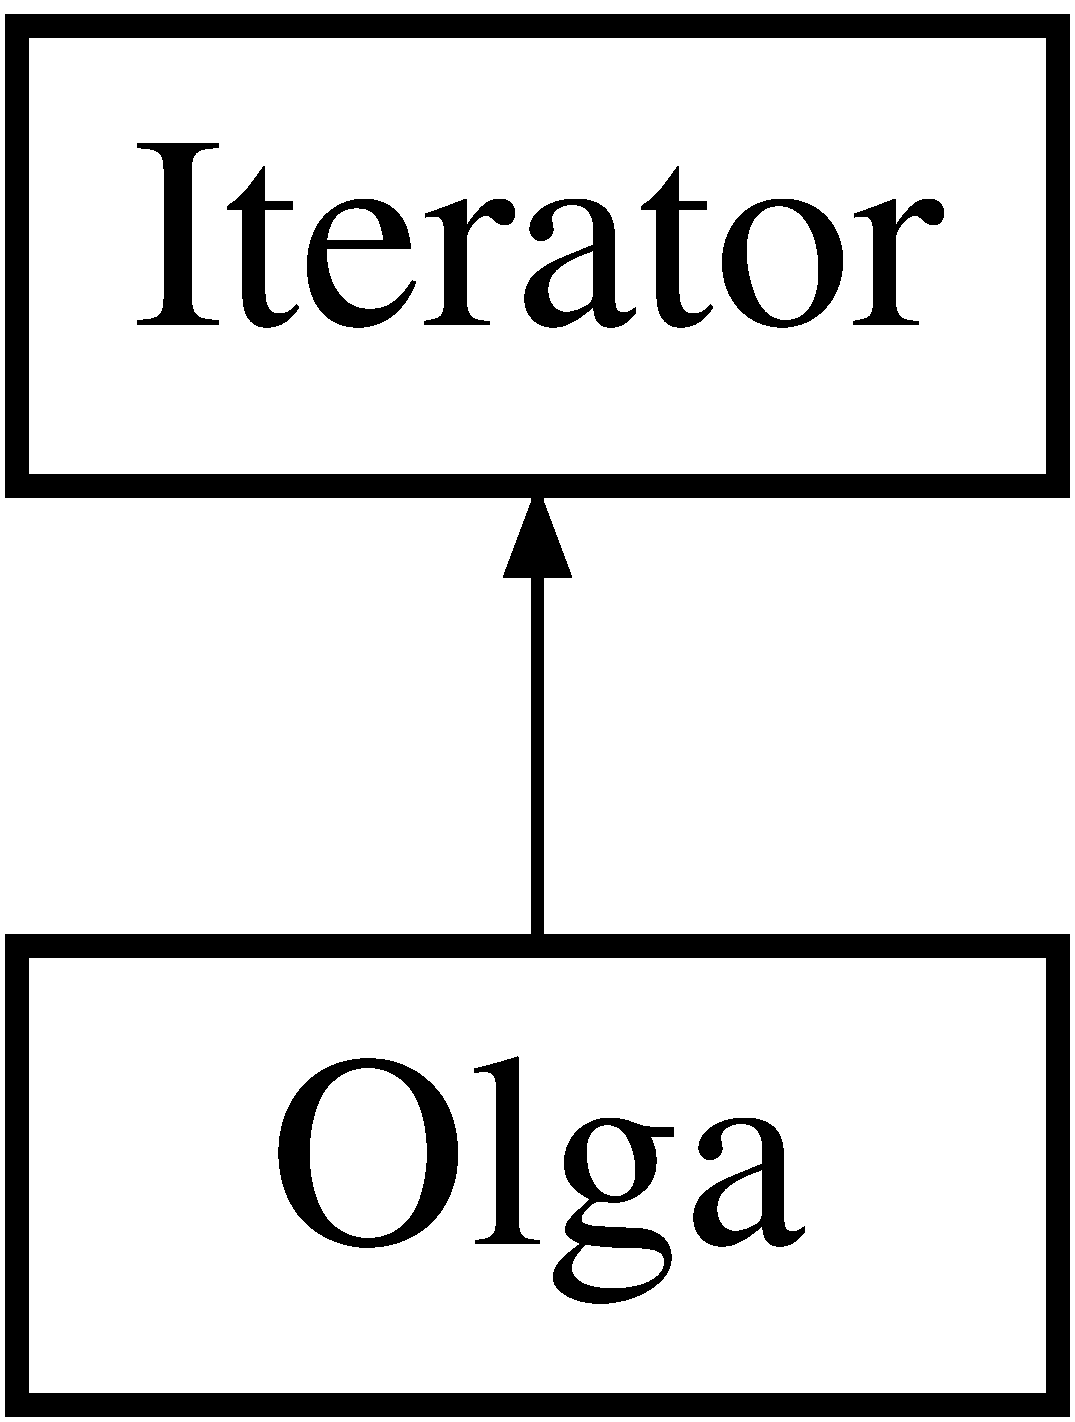
\includegraphics[height=2.000000cm]{classOlga}
\end{center}
\end{figure}
\subsection*{Public Member Functions}
\begin{DoxyCompactItemize}
\item 
\hyperlink{classOlga_ab67e7ac76ef6a557814cd7ac213dc430}{populate\+From\+X\+Cache} ()
\item 
\hyperlink{classOlga_ab8a8d78ed128b8d61de03ea5655b3d56}{populate\+To\+X\+Cache} ()
\item 
\hyperlink{classOlga_ab1486ce669a2e243f9af2f568acb96a5}{populate\+From\+Debby} (\$D\+E\+B)
\item 
\hyperlink{classOlga_a8710c283121a75c551f0beb7eeaf4aa1}{populate\+To\+Debby} ()
\item 
\hyperlink{classOlga_a3ce181004b4dc00140033a7a27eeb747}{load} ()
\item 
\hyperlink{classOlga_a2d4f4e863fd7f9c3e4fee16211b01c53}{save} (\$only\+To\+Memory=\hyperlink{tina4_8php_aec2deb5590a84bee262c3bea206ae88f}{false})
\item 
\hyperlink{classOlga_a83be44e261718dbad296228b541a6c79}{\+\_\+\+\_\+clone} ()
\item 
\hyperlink{classOlga_a183d3f4eab720c297684ccdac5c627b9}{append} (\$\hyperlink{Shape_8php_a774642dc290de09e3aff55c8b594113f}{object})
\item 
\hyperlink{classOlga_af49d06e30d44fab89411ee8994c530fa}{to\+J\+S\+O\+N} ()
\item 
\hyperlink{classOlga_a0f2252c2c92246037adb8ba532e85aef}{from\+J\+S\+O\+N} (\$json\+String)
\item 
\hyperlink{classOlga_a87be848339896b4d554e0189f5ec23d4}{\+\_\+\+\_\+to\+Json} (\$data)
\item 
\hyperlink{classOlga_a44a731386b1e7682cbc3b01c0faef9cd}{\+\_\+\+\_\+call} (\$method, \$args)
\item 
\hyperlink{classOlga_ac2e66056e2619f9bbdafa675702780e2}{persist} ()
\item 
\hyperlink{classOlga_ac08323518a6c8131a357f046b5a0e201}{create\+Get\+Set} ()
\item 
\hyperlink{classOlga_a4688feb4c2a9584030f8f6f3b64bb2db}{\+\_\+\+\_\+construct} (\$json\+String=\char`\"{}\char`\"{})
\item 
\hyperlink{classOlga_abe4a13fb8566761eb44fbed7c4125c14}{current} ()
\item 
\hyperlink{classOlga_a0f70223e5588db45cc81241c78391007}{next} ()
\item 
\hyperlink{classOlga_a2ab85e63c42b998496daf20d89fa8a4a}{key} ()
\item 
\hyperlink{classOlga_a9aaaf12a2bbcd99f876e2e9e1dcac02b}{valid} ()
\item 
\hyperlink{classOlga_ae69d5da6af979c897bd3fcf535d07169}{rewind} ()
\item 
\hyperlink{classOlga_abf255c4baa60ff0847c0ddc8f41d19f1}{count} ()
\item 
\hyperlink{classOlga_af2f971a5c1f12094536bb32eb042e649}{clear} ()
\end{DoxyCompactItemize}
\subsection*{Public Attributes}
\begin{DoxyCompactItemize}
\item 
\hyperlink{classOlga_aeec96cdbc35fcd60afe0a26b4fe49f6e}{\$array\+Objects} = \mbox{[}$\,$\mbox{]}
\end{DoxyCompactItemize}


\subsection{Detailed Description}
\hyperlink{classOlga}{Olga} is a class which adds getters and setters to your existing object, it has methods to export the class to J\+S\+O\+N and to import the class from J\+S\+O\+N User\+: Andre van Zuydam Date\+: 2015-\/09-\/04 Time\+: 04\+:05 P\+M 

\subsection{Constructor \& Destructor Documentation}
\hypertarget{classOlga_a4688feb4c2a9584030f8f6f3b64bb2db}{}\index{Olga@{Olga}!\+\_\+\+\_\+construct@{\+\_\+\+\_\+construct}}
\index{\+\_\+\+\_\+construct@{\+\_\+\+\_\+construct}!Olga@{Olga}}
\subsubsection[{\+\_\+\+\_\+construct}]{\setlength{\rightskip}{0pt plus 5cm}Olga\+::\+\_\+\+\_\+construct (
\begin{DoxyParamCaption}
\item[{}]{\$json\+String = {\ttfamily \char`\"{}\char`\"{}}}
\end{DoxyParamCaption}
)}\label{classOlga_a4688feb4c2a9584030f8f6f3b64bb2db}
Constructor to make getters and setters 

\subsection{Member Function Documentation}
\hypertarget{classOlga_a44a731386b1e7682cbc3b01c0faef9cd}{}\index{Olga@{Olga}!\+\_\+\+\_\+call@{\+\_\+\+\_\+call}}
\index{\+\_\+\+\_\+call@{\+\_\+\+\_\+call}!Olga@{Olga}}
\subsubsection[{\+\_\+\+\_\+call}]{\setlength{\rightskip}{0pt plus 5cm}Olga\+::\+\_\+\+\_\+call (
\begin{DoxyParamCaption}
\item[{}]{\$method, }
\item[{}]{\$args}
\end{DoxyParamCaption}
)}\label{classOlga_a44a731386b1e7682cbc3b01c0faef9cd}
Call the dynamically instantiated getters \& setters 
\begin{DoxyParams}{Parameters}
{\em \$method} & \\
\hline
{\em \$args} & \\
\hline
\end{DoxyParams}
\begin{DoxyReturn}{Returns}
mixed 
\end{DoxyReturn}
\hypertarget{classOlga_a83be44e261718dbad296228b541a6c79}{}\index{Olga@{Olga}!\+\_\+\+\_\+clone@{\+\_\+\+\_\+clone}}
\index{\+\_\+\+\_\+clone@{\+\_\+\+\_\+clone}!Olga@{Olga}}
\subsubsection[{\+\_\+\+\_\+clone}]{\setlength{\rightskip}{0pt plus 5cm}Olga\+::\+\_\+\+\_\+clone (
\begin{DoxyParamCaption}
{}
\end{DoxyParamCaption}
)}\label{classOlga_a83be44e261718dbad296228b541a6c79}
The clone function must recreate the object closures \hypertarget{classOlga_a87be848339896b4d554e0189f5ec23d4}{}\index{Olga@{Olga}!\+\_\+\+\_\+to\+Json@{\+\_\+\+\_\+to\+Json}}
\index{\+\_\+\+\_\+to\+Json@{\+\_\+\+\_\+to\+Json}!Olga@{Olga}}
\subsubsection[{\+\_\+\+\_\+to\+Json}]{\setlength{\rightskip}{0pt plus 5cm}Olga\+::\+\_\+\+\_\+to\+Json (
\begin{DoxyParamCaption}
\item[{}]{\$data}
\end{DoxyParamCaption}
)}\label{classOlga_a87be848339896b4d554e0189f5ec23d4}
Custom Object J\+S\+O\+N encoder, thanks to boukeversteegh at gmail dot com, modified by Andre van Zuydam to ignore dynamic getters and setters 
\begin{DoxyParams}{Parameters}
{\em \$data} & \\
\hline
\end{DoxyParams}
\begin{DoxyReturn}{Returns}
string 
\end{DoxyReturn}
\hypertarget{classOlga_a183d3f4eab720c297684ccdac5c627b9}{}\index{Olga@{Olga}!append@{append}}
\index{append@{append}!Olga@{Olga}}
\subsubsection[{append}]{\setlength{\rightskip}{0pt plus 5cm}Olga\+::append (
\begin{DoxyParamCaption}
\item[{}]{\$object}
\end{DoxyParamCaption}
)}\label{classOlga_a183d3f4eab720c297684ccdac5c627b9}
Append an object that has similar properties as the known object \hypertarget{classOlga_af2f971a5c1f12094536bb32eb042e649}{}\index{Olga@{Olga}!clear@{clear}}
\index{clear@{clear}!Olga@{Olga}}
\subsubsection[{clear}]{\setlength{\rightskip}{0pt plus 5cm}Olga\+::clear (
\begin{DoxyParamCaption}
{}
\end{DoxyParamCaption}
)}\label{classOlga_af2f971a5c1f12094536bb32eb042e649}
Method to clear all the objects from the system \begin{DoxyReturn}{Returns}
bool 
\end{DoxyReturn}
\hypertarget{classOlga_abf255c4baa60ff0847c0ddc8f41d19f1}{}\index{Olga@{Olga}!count@{count}}
\index{count@{count}!Olga@{Olga}}
\subsubsection[{count}]{\setlength{\rightskip}{0pt plus 5cm}Olga\+::count (
\begin{DoxyParamCaption}
{}
\end{DoxyParamCaption}
)}\label{classOlga_abf255c4baa60ff0847c0ddc8f41d19f1}
Give a count of the records in the object \begin{DoxyReturn}{Returns}
int 
\end{DoxyReturn}
\hypertarget{classOlga_ac08323518a6c8131a357f046b5a0e201}{}\index{Olga@{Olga}!create\+Get\+Set@{create\+Get\+Set}}
\index{create\+Get\+Set@{create\+Get\+Set}!Olga@{Olga}}
\subsubsection[{create\+Get\+Set}]{\setlength{\rightskip}{0pt plus 5cm}Olga\+::create\+Get\+Set (
\begin{DoxyParamCaption}
{}
\end{DoxyParamCaption}
)}\label{classOlga_ac08323518a6c8131a357f046b5a0e201}
Create the getters \& setters \hypertarget{classOlga_abe4a13fb8566761eb44fbed7c4125c14}{}\index{Olga@{Olga}!current@{current}}
\index{current@{current}!Olga@{Olga}}
\subsubsection[{current}]{\setlength{\rightskip}{0pt plus 5cm}Olga\+::current (
\begin{DoxyParamCaption}
{}
\end{DoxyParamCaption}
)}\label{classOlga_abe4a13fb8566761eb44fbed7c4125c14}
Return the current element \hyperlink{}{mixed Can return any type.  5.\+0.\+0 }\hypertarget{classOlga_a0f2252c2c92246037adb8ba532e85aef}{}\index{Olga@{Olga}!from\+J\+S\+O\+N@{from\+J\+S\+O\+N}}
\index{from\+J\+S\+O\+N@{from\+J\+S\+O\+N}!Olga@{Olga}}
\subsubsection[{from\+J\+S\+O\+N}]{\setlength{\rightskip}{0pt plus 5cm}Olga\+::from\+J\+S\+O\+N (
\begin{DoxyParamCaption}
\item[{}]{\$json\+String}
\end{DoxyParamCaption}
)}\label{classOlga_a0f2252c2c92246037adb8ba532e85aef}
Converts a J\+S\+O\+N strings values to the current object for instantiating the object 
\begin{DoxyParams}{Parameters}
{\em \$json\+String} & \\
\hline
\end{DoxyParams}
\hypertarget{classOlga_a2ab85e63c42b998496daf20d89fa8a4a}{}\index{Olga@{Olga}!key@{key}}
\index{key@{key}!Olga@{Olga}}
\subsubsection[{key}]{\setlength{\rightskip}{0pt plus 5cm}Olga\+::key (
\begin{DoxyParamCaption}
{}
\end{DoxyParamCaption}
)}\label{classOlga_a2ab85e63c42b998496daf20d89fa8a4a}
Return the key of the current element \hyperlink{}{mixed scalar on success, or null on failure.  5.\+0.\+0 }\hypertarget{classOlga_a3ce181004b4dc00140033a7a27eeb747}{}\index{Olga@{Olga}!load@{load}}
\index{load@{load}!Olga@{Olga}}
\subsubsection[{load}]{\setlength{\rightskip}{0pt plus 5cm}Olga\+::load (
\begin{DoxyParamCaption}
{}
\end{DoxyParamCaption}
)}\label{classOlga_a3ce181004b4dc00140033a7a27eeb747}
A method to load the data from the database into the object in question \hypertarget{classOlga_a0f70223e5588db45cc81241c78391007}{}\index{Olga@{Olga}!next@{next}}
\index{next@{next}!Olga@{Olga}}
\subsubsection[{next}]{\setlength{\rightskip}{0pt plus 5cm}Olga\+::next (
\begin{DoxyParamCaption}
{}
\end{DoxyParamCaption}
)}\label{classOlga_a0f70223e5588db45cc81241c78391007}
Move forward to next element \hyperlink{}{void Any returned value is ignored.  5.\+0.\+0 }\hypertarget{classOlga_ac2e66056e2619f9bbdafa675702780e2}{}\index{Olga@{Olga}!persist@{persist}}
\index{persist@{persist}!Olga@{Olga}}
\subsubsection[{persist}]{\setlength{\rightskip}{0pt plus 5cm}Olga\+::persist (
\begin{DoxyParamCaption}
{}
\end{DoxyParamCaption}
)}\label{classOlga_ac2e66056e2619f9bbdafa675702780e2}
\hypertarget{classOlga_ab1486ce669a2e243f9af2f568acb96a5}{}\index{Olga@{Olga}!populate\+From\+Debby@{populate\+From\+Debby}}
\index{populate\+From\+Debby@{populate\+From\+Debby}!Olga@{Olga}}
\subsubsection[{populate\+From\+Debby}]{\setlength{\rightskip}{0pt plus 5cm}Olga\+::populate\+From\+Debby (
\begin{DoxyParamCaption}
\item[{}]{\$\+D\+E\+B}
\end{DoxyParamCaption}
)}\label{classOlga_ab1486ce669a2e243f9af2f568acb96a5}
Method to get the results from the database \hypertarget{classOlga_ab67e7ac76ef6a557814cd7ac213dc430}{}\index{Olga@{Olga}!populate\+From\+X\+Cache@{populate\+From\+X\+Cache}}
\index{populate\+From\+X\+Cache@{populate\+From\+X\+Cache}!Olga@{Olga}}
\subsubsection[{populate\+From\+X\+Cache}]{\setlength{\rightskip}{0pt plus 5cm}Olga\+::populate\+From\+X\+Cache (
\begin{DoxyParamCaption}
{}
\end{DoxyParamCaption}
)}\label{classOlga_ab67e7ac76ef6a557814cd7ac213dc430}
Method to get the results from X\+Cache into the object \hypertarget{classOlga_a8710c283121a75c551f0beb7eeaf4aa1}{}\index{Olga@{Olga}!populate\+To\+Debby@{populate\+To\+Debby}}
\index{populate\+To\+Debby@{populate\+To\+Debby}!Olga@{Olga}}
\subsubsection[{populate\+To\+Debby}]{\setlength{\rightskip}{0pt plus 5cm}Olga\+::populate\+To\+Debby (
\begin{DoxyParamCaption}
{}
\end{DoxyParamCaption}
)}\label{classOlga_a8710c283121a75c551f0beb7eeaf4aa1}
Method to update the database from the objects in memory \begin{DoxyReturn}{Returns}
bool 
\end{DoxyReturn}
\hypertarget{classOlga_ab8a8d78ed128b8d61de03ea5655b3d56}{}\index{Olga@{Olga}!populate\+To\+X\+Cache@{populate\+To\+X\+Cache}}
\index{populate\+To\+X\+Cache@{populate\+To\+X\+Cache}!Olga@{Olga}}
\subsubsection[{populate\+To\+X\+Cache}]{\setlength{\rightskip}{0pt plus 5cm}Olga\+::populate\+To\+X\+Cache (
\begin{DoxyParamCaption}
{}
\end{DoxyParamCaption}
)}\label{classOlga_ab8a8d78ed128b8d61de03ea5655b3d56}
Method to put the results into the xcache \hypertarget{classOlga_ae69d5da6af979c897bd3fcf535d07169}{}\index{Olga@{Olga}!rewind@{rewind}}
\index{rewind@{rewind}!Olga@{Olga}}
\subsubsection[{rewind}]{\setlength{\rightskip}{0pt plus 5cm}Olga\+::rewind (
\begin{DoxyParamCaption}
{}
\end{DoxyParamCaption}
)}\label{classOlga_ae69d5da6af979c897bd3fcf535d07169}
Rewind the Iterator to the first element \hyperlink{}{void Any returned value is ignored.  5.\+0.\+0 }\hypertarget{classOlga_a2d4f4e863fd7f9c3e4fee16211b01c53}{}\index{Olga@{Olga}!save@{save}}
\index{save@{save}!Olga@{Olga}}
\subsubsection[{save}]{\setlength{\rightskip}{0pt plus 5cm}Olga\+::save (
\begin{DoxyParamCaption}
\item[{}]{\$only\+To\+Memory = {\ttfamily {\bf false}}}
\end{DoxyParamCaption}
)}\label{classOlga_a2d4f4e863fd7f9c3e4fee16211b01c53}
A method to save the data into the database from the object in question 
\begin{DoxyParams}[1]{Parameters}
bool | false & {\em \$only\+To\+Memory} & Saves only to memory \\
\hline
\end{DoxyParams}
\begin{DoxyReturn}{Returns}
bool 
\end{DoxyReturn}
\hypertarget{classOlga_af49d06e30d44fab89411ee8994c530fa}{}\index{Olga@{Olga}!to\+J\+S\+O\+N@{to\+J\+S\+O\+N}}
\index{to\+J\+S\+O\+N@{to\+J\+S\+O\+N}!Olga@{Olga}}
\subsubsection[{to\+J\+S\+O\+N}]{\setlength{\rightskip}{0pt plus 5cm}Olga\+::to\+J\+S\+O\+N (
\begin{DoxyParamCaption}
{}
\end{DoxyParamCaption}
)}\label{classOlga_af49d06e30d44fab89411ee8994c530fa}
Create a J\+S\+O\+N instance of the object \begin{DoxyReturn}{Returns}
string 
\end{DoxyReturn}
\hypertarget{classOlga_a9aaaf12a2bbcd99f876e2e9e1dcac02b}{}\index{Olga@{Olga}!valid@{valid}}
\index{valid@{valid}!Olga@{Olga}}
\subsubsection[{valid}]{\setlength{\rightskip}{0pt plus 5cm}Olga\+::valid (
\begin{DoxyParamCaption}
{}
\end{DoxyParamCaption}
)}\label{classOlga_a9aaaf12a2bbcd99f876e2e9e1dcac02b}
Checks if current position is valid \hyperlink{}{boolean The return value will be casted to boolean and then evaluated. Returns true on success or false on failure.  5.\+0.\+0 }

\subsection{Member Data Documentation}
\hypertarget{classOlga_aeec96cdbc35fcd60afe0a26b4fe49f6e}{}\index{Olga@{Olga}!\$array\+Objects@{\$array\+Objects}}
\index{\$array\+Objects@{\$array\+Objects}!Olga@{Olga}}
\subsubsection[{\$array\+Objects}]{\setlength{\rightskip}{0pt plus 5cm}Olga\+::\$array\+Objects = \mbox{[}$\,$\mbox{]}}\label{classOlga_aeec96cdbc35fcd60afe0a26b4fe49f6e}


The documentation for this class was generated from the following file\+:\begin{DoxyCompactItemize}
\item 
web\+\_\+root/tina4/\hyperlink{Olga_8php}{Olga.\+php}\end{DoxyCompactItemize}

\hypertarget{classPhoebe}{}\section{Phoebe Class Reference}
\label{classPhoebe}\index{Phoebe@{Phoebe}}
\subsection*{Public Member Functions}
\begin{DoxyCompactItemize}
\item 
\hyperlink{classPhoebe_a213905140234c1d4707bc780319eb0b5}{\+\_\+\+\_\+construct} (\$phar\+Name)
\end{DoxyCompactItemize}


\subsection{Detailed Description}
Description of \hyperlink{classPhoebe}{Phoebe}

\begin{DoxyAuthor}{Author}
Andre van Zuydam \href{mailto:andre@xineoh.com}{\tt andre@xineoh.\+com} 
\end{DoxyAuthor}


\subsection{Constructor \& Destructor Documentation}
\hypertarget{classPhoebe_a213905140234c1d4707bc780319eb0b5}{}\index{Phoebe@{Phoebe}!\+\_\+\+\_\+construct@{\+\_\+\+\_\+construct}}
\index{\+\_\+\+\_\+construct@{\+\_\+\+\_\+construct}!Phoebe@{Phoebe}}
\subsubsection[{\+\_\+\+\_\+construct}]{\setlength{\rightskip}{0pt plus 5cm}Phoebe\+::\+\_\+\+\_\+construct (
\begin{DoxyParamCaption}
\item[{}]{\$phar\+Name}
\end{DoxyParamCaption}
)}\label{classPhoebe_a213905140234c1d4707bc780319eb0b5}


The documentation for this class was generated from the following file\+:\begin{DoxyCompactItemize}
\item 
web\+\_\+root/tina4/\hyperlink{Phoebe_8php}{Phoebe.\+php}\end{DoxyCompactItemize}

\hypertarget{classReta}{}\section{Reta Class Reference}
\label{classReta}\index{Reta@{Reta}}
\subsection*{Public Member Functions}
\begin{DoxyCompactItemize}
\item 
\hyperlink{classReta_a59ebb4d8111b19bcc2b646352035f88a}{\+\_\+\+\_\+construct} (\$report\+Path=\char`\"{}reports\char`\"{}, \$output\+Path=\char`\"{}output\char`\"{}, \$ini\+File=\char`\"{}reta.\+ini\char`\"{}, \$reta\+Path=\char`\"{}\char`\"{})
\item 
\hyperlink{classReta_a7e909b970b993508a9ff7a5361a58032}{generate} (\$report\+Name=\char`\"{}test\char`\"{}, \$sql, \$output\+Type=\char`\"{}pdf,csv\char`\"{}, \$debug=false)
\end{DoxyCompactItemize}


\subsection{Detailed Description}
\hyperlink{classReta}{Reta} makes the reporting possible by using the open source engine of Report Manager \hyperlink{classReta}{Reta} requires wine to run on Linux and uses the reta.\+sh shell wrapper

Currently supported database engines are\+: sqlite3, firebird-\/2.\+5, mysql

\begin{DoxyAuthor}{Author}
Andre van Zuydam \href{mailto:andre@xineoh.com}{\tt andre@xineoh.\+com} 
\end{DoxyAuthor}


\subsection{Constructor \& Destructor Documentation}
\hypertarget{classReta_a59ebb4d8111b19bcc2b646352035f88a}{}\index{Reta@{Reta}!\+\_\+\+\_\+construct@{\+\_\+\+\_\+construct}}
\index{\+\_\+\+\_\+construct@{\+\_\+\+\_\+construct}!Reta@{Reta}}
\subsubsection[{\+\_\+\+\_\+construct}]{\setlength{\rightskip}{0pt plus 5cm}Reta\+::\+\_\+\+\_\+construct (
\begin{DoxyParamCaption}
\item[{}]{\$report\+Path = {\ttfamily \char`\"{}reports\char`\"{}}, }
\item[{}]{\$output\+Path = {\ttfamily \char`\"{}output\char`\"{}}, }
\item[{}]{\$ini\+File = {\ttfamily \char`\"{}reta.ini\char`\"{}}, }
\item[{}]{\$reta\+Path = {\ttfamily \char`\"{}\char`\"{}}}
\end{DoxyParamCaption}
)}\label{classReta_a59ebb4d8111b19bcc2b646352035f88a}
The constructor for \hyperlink{classReta}{Reta} 
\begin{DoxyParams}[1]{Parameters}
String & {\em \$report\+Path} & Relative to the document root \\
\hline
String & {\em \$output\+Path} & Relative to the document root \\
\hline
String & {\em \$ini\+File} & Path to the ini\+File, normally is in the same folder as reta, but you may want more. \\
\hline
String & {\em \$reta\+Path} & Path to reta if the system can\textquotesingle{}t determine it, usually one folder below the document root \\
\hline
\end{DoxyParams}


\subsection{Member Function Documentation}
\hypertarget{classReta_a7e909b970b993508a9ff7a5361a58032}{}\index{Reta@{Reta}!generate@{generate}}
\index{generate@{generate}!Reta@{Reta}}
\subsubsection[{generate}]{\setlength{\rightskip}{0pt plus 5cm}Reta\+::generate (
\begin{DoxyParamCaption}
\item[{}]{\$report\+Name = {\ttfamily \char`\"{}test\char`\"{}}, }
\item[{}]{\$sql, }
\item[{}]{\$output\+Type = {\ttfamily \char`\"{}pdf,csv\char`\"{}}, }
\item[{}]{\$debug = {\ttfamily false}}
\end{DoxyParamCaption}
)}\label{classReta_a7e909b970b993508a9ff7a5361a58032}
generate calls the rita engine to generate the report. 
\begin{DoxyParams}[1]{Parameters}
String & {\em \$report\+Name} & The name of the report file without the rep extension \\
\hline
String & {\em \$sql} & A valid S\+Q\+L statement which will work with the database \\
\hline
String & {\em \$output\+Type} & A comma separated string which can include \+: pdf,csv,xls,html \\
\hline
Boolean & {\em \$debug} & Turn on the debugging messages for troubleshooting \\
\hline
\end{DoxyParams}


The documentation for this class was generated from the following file\+:\begin{DoxyCompactItemize}
\item 
web\+\_\+root/tina4/\hyperlink{Reta_8php}{Reta.\+php}\end{DoxyCompactItemize}

\hypertarget{classRuth}{}\section{Ruth Class Reference}
\label{classRuth}\index{Ruth@{Ruth}}
\subsection*{Static Public Member Functions}
\begin{DoxyCompactItemize}
\item 
static \hyperlink{classRuth_a0d04b422b261fcbf033abfe6b77d5a2d}{auto\+Load} (\$paths, \$load\+Auto\+Load=true, \$ignore\+Requires=false)
\item 
static \hyperlink{classRuth_a6322471f9832f6b0c92e8d321956874c}{Message} (\$\hyperlink{Tessa_8php_a37ab31c170417027f819bfc053d7cd39}{message})
\item 
static \hyperlink{classRuth_aa0e8f0a163756675b0ec431bb7dd0b49}{D\+E\+B\+U\+G} ()
\item 
static \hyperlink{classRuth_a0fc75ae6b986d7109f66f659cf1dcac2}{set\+R\+E\+Q\+U\+E\+S\+T} (\$key\+Name=\char`\"{}\char`\"{}, \$key\+Value=\char`\"{}\char`\"{})
\item 
static \hyperlink{classRuth_abe809de9dafced3724124f3399af01f3}{get\+R\+E\+Q\+U\+E\+S\+T} (\$key\+Name=\char`\"{}\char`\"{})
\item 
static \hyperlink{classRuth_a0a05421198533990654d0c1fb0beaffd}{get\+R\+E\+Q\+U\+E\+S\+T\+\_\+\+U\+R\+I} ()
\item 
static \hyperlink{classRuth_a627fd70f5f186ba0d4d3dc187a432b81}{request\+To\+S\+E\+S\+S\+I\+O\+N} (\$filter=\char`\"{}\char`\"{})
\item 
static \hyperlink{classRuth_ae10d9c25d1910e59a15662dd1304c23b}{request\+To\+Input} (\$type=\char`\"{}hidden\char`\"{}, \$filter=null)
\item 
static \hyperlink{classRuth_addbd05bd71b3abeff8e8250c46897e5b}{get\+P\+O\+S\+T\+\_\+\+D\+A\+T\+A} ()
\item 
static \hyperlink{classRuth_a899c68457a6a7c1b8a0b25bfd74c4c15}{get\+O\+B\+J\+E\+C\+T} (\$key\+Name=\char`\"{}\char`\"{})
\item 
static \hyperlink{classRuth_a9d554d9bdfe7596d41a2b08a3c0db9ce}{set\+O\+B\+J\+E\+C\+T} (\$name, \$\hyperlink{Shape_8php_a774642dc290de09e3aff55c8b594113f}{object})
\item 
static \hyperlink{classRuth_a971920e4c13f4e16bc8d72379804c16f}{set\+C\+O\+O\+K\+I\+E} (\$cookie\+Name, \$value=\char`\"{}\char`\"{}, \$minutes=60)
\item 
static \hyperlink{classRuth_a5ec6c65c94d056a2e0705efaa56f7660}{get\+C\+O\+O\+K\+I\+E} (\$key\+Name=\char`\"{}\char`\"{})
\item 
static \hyperlink{classRuth_a12be6f40ae06f4443848d0f8a089bd00}{get\+F\+I\+L\+E\+S} (\$key\+Name=\char`\"{}\char`\"{})
\item 
static \hyperlink{classRuth_ab868231ae3b29da9c9456d0b866dc8ec}{get\+S\+E\+R\+V\+E\+R} (\$key\+Name=\char`\"{}\char`\"{})
\item 
static \hyperlink{classRuth_abbbe520ef7554c895ab5f4213b8738a3}{get\+P\+A\+T\+H} ()
\item 
static \hyperlink{classRuth_a258953d4afe38d92f4be70313d500d40}{get\+R\+E\+A\+L\+\_\+\+P\+A\+T\+H} ()
\item 
static \hyperlink{classRuth_a0801b3a28f3385eeee817a3deb14b028}{get\+D\+O\+C\+U\+M\+E\+N\+T\+\_\+\+R\+O\+O\+T} ()
\item 
static \hyperlink{classRuth_a692691e58b9b2fce80e0bed5a3207137}{get\+L\+A\+S\+T\+R\+O\+U\+T\+E} (\$request\+Method=\char`\"{}\char`\"{})
\item 
static \hyperlink{classRuth_a4a88a74e5af0a0155eb3fe438ad995c3}{set\+S\+E\+S\+S\+I\+O\+N} (\$key\+Name=\char`\"{}\char`\"{}, \$key\+Value=\char`\"{}\char`\"{})
\item 
static \hyperlink{classRuth_a0960ac91d1a1ce9c7cb3324ee51f4d74}{get\+S\+E\+S\+S\+I\+O\+N} (\$key\+Name=\char`\"{}\char`\"{})
\item 
static \hyperlink{classRuth_a4f4e6184de654b141a679146e35f8f59}{unset\+S\+E\+S\+S\+I\+O\+N} (\$key\+Name=\char`\"{}\char`\"{})
\item 
static \hyperlink{classRuth_a169d4a654420b5abce66787cc8cb51b4}{set\+R\+O\+L\+E} (\$role\+Name=\char`\"{}\char`\"{}, \$routes\+Allowed=\char`\"{}\char`\"{}, \$default\+Role=false)
\item 
static \hyperlink{classRuth_a2cbe3cd7c0d3dfadac54a6020d075607}{set\+Authorization} (\$role\+Name=\char`\"{}\char`\"{}, \$auth\+D\+A\+T\+A=\char`\"{}\char`\"{}, \$life\+Time=30)
\item 
static \hyperlink{classRuth_af751cee7c3766c478a09ea14ffc5ce99}{del\+Authorization} ()
\item 
static \hyperlink{classRuth_a2ce840061c470dee079816ec54bfc1f4}{init\+Ruth} (\$session\+Name)
\item 
static \hyperlink{classRuth_ad13bc87f60f8b74efd4c784fa2c49288}{add\+Route} (\$request\+Method, \$route\+Path, \$route\+Function, \$custom\+Params=\char`\"{}\char`\"{}, \$route\+Ignore\+Tracking=false)
\item 
static \hyperlink{classRuth_a824d3cd236fd20d3f8cdc1865b8a3605}{add\+Error\+Route} (\$error\+Code, \$route\+Path)
\item 
static \hyperlink{classRuth_aba8f6d2223ff063fc5d0133d6f85f2c0}{response\+Header} (\$error\+Code=404, \$\hyperlink{Tessa_8php_a37ab31c170417027f819bfc053d7cd39}{message}=\char`\"{}\char`\"{})
\item 
static \hyperlink{classRuth_af382f8396d9d15c9d289b1024a974360}{create\+Reg\+Ex} (\$route\+Path)
\item 
static \hyperlink{classRuth_a4cc98adb973c4d46742b05a02ecb6ee3}{match\+Route} (\$route\+Path, \$U\+R\+I)
\item 
static \hyperlink{classRuth_aa8c09285cc5f2a214b8fbe5e45e88cea}{get\+Params} (\$route\+Path, \$U\+R\+I)
\item 
static \hyperlink{classRuth_a99efe91394d300de83f7124acea0b595}{redirect} (\$new\+Path=\char`\"{}\char`\"{})
\item 
static \hyperlink{classRuth_aa9bd38599bb5bd892ddf856c1687b04a}{get\+Authorization} (\$route\+Path=\char`\"{}\char`\"{})
\item 
static \hyperlink{classRuth_a0fbc42c3af4f62e230b4c3208ce9451c}{parse\+Routes} (\$custom\+Path=\char`\"{}\char`\"{})
\end{DoxyCompactItemize}


\subsection{Member Function Documentation}
\hypertarget{classRuth_a824d3cd236fd20d3f8cdc1865b8a3605}{}\index{Ruth@{Ruth}!add\+Error\+Route@{add\+Error\+Route}}
\index{add\+Error\+Route@{add\+Error\+Route}!Ruth@{Ruth}}
\subsubsection[{add\+Error\+Route}]{\setlength{\rightskip}{0pt plus 5cm}static Ruth\+::add\+Error\+Route (
\begin{DoxyParamCaption}
\item[{}]{\$error\+Code, }
\item[{}]{\$route\+Path}
\end{DoxyParamCaption}
)\hspace{0.3cm}{\ttfamily [static]}}\label{classRuth_a824d3cd236fd20d3f8cdc1865b8a3605}
This is where you add custom routes for H\+T\+M\+L error codes, they should be already defined via add\+Route in order to work


\begin{DoxyParams}[1]{Parameters}
Integer & {\em \$error\+Code} & A valid H\+T\+M\+L error code \\
\hline
String & {\em \$route\+Path} & A valid route for \hyperlink{classRuth}{Ruth} to redirect to \\
\hline
\end{DoxyParams}
\begin{DoxyReturn}{Returns}
boolean 
\end{DoxyReturn}
\hypertarget{classRuth_ad13bc87f60f8b74efd4c784fa2c49288}{}\index{Ruth@{Ruth}!add\+Route@{add\+Route}}
\index{add\+Route@{add\+Route}!Ruth@{Ruth}}
\subsubsection[{add\+Route}]{\setlength{\rightskip}{0pt plus 5cm}static Ruth\+::add\+Route (
\begin{DoxyParamCaption}
\item[{}]{\$request\+Method, }
\item[{}]{\$route\+Path, }
\item[{}]{\$route\+Function, }
\item[{}]{\$custom\+Params = {\ttfamily \char`\"{}\char`\"{}}, }
\item[{}]{\$route\+Ignore\+Tracking = {\ttfamily false}}
\end{DoxyParamCaption}
)\hspace{0.3cm}{\ttfamily [static]}}\label{classRuth_ad13bc87f60f8b74efd4c784fa2c49288}
The Add Route Method

This method adds routes into the system based on what the user wants to use, your webserver needs to be configured correctly for this to work.


\begin{DoxyParams}[1]{Parameters}
String & {\em \$request\+Method} & Either G\+E\+T, P\+U\+T, P\+O\+S\+T, D\+E\+L\+E\+T\+E \\
\hline
String & {\em \$route\+Path} & A path to be used as a route, eg. /user, variables can also be parsed /user/\{id\}/ and wildcards are $\ast$ \\
\hline
Function & {\em \$route\+Function} & A function which will be called with the corresponding variables \\
\hline
Boolean & {\em \$route\+Ignore\+Tracking} & \hyperlink{classRuth}{Ruth} uses this to give you back the last route but you may not want her to remember all the paths \\
\hline
\end{DoxyParams}
\begin{DoxyReturn}{Returns}
Boolean Always returns true 
\end{DoxyReturn}
\hypertarget{classRuth_a0d04b422b261fcbf033abfe6b77d5a2d}{}\index{Ruth@{Ruth}!auto\+Load@{auto\+Load}}
\index{auto\+Load@{auto\+Load}!Ruth@{Ruth}}
\subsubsection[{auto\+Load}]{\setlength{\rightskip}{0pt plus 5cm}static Ruth\+::auto\+Load (
\begin{DoxyParamCaption}
\item[{}]{\$paths, }
\item[{}]{\$load\+Auto\+Load = {\ttfamily true}, }
\item[{}]{\$ignore\+Requires = {\ttfamily false}}
\end{DoxyParamCaption}
)\hspace{0.3cm}{\ttfamily [static]}}\label{classRuth_a0d04b422b261fcbf033abfe6b77d5a2d}
Auto Load tries to include new class requires automatically \hypertarget{classRuth_af382f8396d9d15c9d289b1024a974360}{}\index{Ruth@{Ruth}!create\+Reg\+Ex@{create\+Reg\+Ex}}
\index{create\+Reg\+Ex@{create\+Reg\+Ex}!Ruth@{Ruth}}
\subsubsection[{create\+Reg\+Ex}]{\setlength{\rightskip}{0pt plus 5cm}static Ruth\+::create\+Reg\+Ex (
\begin{DoxyParamCaption}
\item[{}]{\$route\+Path}
\end{DoxyParamCaption}
)\hspace{0.3cm}{\ttfamily [static]}}\label{classRuth_af382f8396d9d15c9d289b1024a974360}
Creates a regular expression

This method created a regular expression to be used for matching with the routing and security


\begin{DoxyParams}[1]{Parameters}
type & {\em \$route\+Path} & The path specified by the user \\
\hline
\end{DoxyParams}
\begin{DoxyReturn}{Returns}
String A regular expression which can be used for routing 
\end{DoxyReturn}
\hypertarget{classRuth_aa0e8f0a163756675b0ec431bb7dd0b49}{}\index{Ruth@{Ruth}!D\+E\+B\+U\+G@{D\+E\+B\+U\+G}}
\index{D\+E\+B\+U\+G@{D\+E\+B\+U\+G}!Ruth@{Ruth}}
\subsubsection[{D\+E\+B\+U\+G}]{\setlength{\rightskip}{0pt plus 5cm}static Ruth\+::\+D\+E\+B\+U\+G (
\begin{DoxyParamCaption}
{}
\end{DoxyParamCaption}
)\hspace{0.3cm}{\ttfamily [static]}}\label{classRuth_aa0e8f0a163756675b0ec431bb7dd0b49}
Switch debugging on for \hyperlink{classRuth}{Ruth}

Turns on the debugging in \hyperlink{classRuth}{Ruth} showing a user how the routing is done \hypertarget{classRuth_af751cee7c3766c478a09ea14ffc5ce99}{}\index{Ruth@{Ruth}!del\+Authorization@{del\+Authorization}}
\index{del\+Authorization@{del\+Authorization}!Ruth@{Ruth}}
\subsubsection[{del\+Authorization}]{\setlength{\rightskip}{0pt plus 5cm}static Ruth\+::del\+Authorization (
\begin{DoxyParamCaption}
{}
\end{DoxyParamCaption}
)\hspace{0.3cm}{\ttfamily [static]}}\label{classRuth_af751cee7c3766c478a09ea14ffc5ce99}
Deletes the security token

The session is invalidated and the internal session variable of \hyperlink{classRuth}{Ruth} updated

\begin{DoxyReturn}{Returns}
Boolean Returns true if there was a non empty auth\+Token in the session 
\end{DoxyReturn}
\hypertarget{classRuth_aa9bd38599bb5bd892ddf856c1687b04a}{}\index{Ruth@{Ruth}!get\+Authorization@{get\+Authorization}}
\index{get\+Authorization@{get\+Authorization}!Ruth@{Ruth}}
\subsubsection[{get\+Authorization}]{\setlength{\rightskip}{0pt plus 5cm}static Ruth\+::get\+Authorization (
\begin{DoxyParamCaption}
\item[{}]{\$route\+Path = {\ttfamily \char`\"{}\char`\"{}}}
\end{DoxyParamCaption}
)\hspace{0.3cm}{\ttfamily [static]}}\label{classRuth_aa9bd38599bb5bd892ddf856c1687b04a}
\hypertarget{classRuth_a5ec6c65c94d056a2e0705efaa56f7660}{}\index{Ruth@{Ruth}!get\+C\+O\+O\+K\+I\+E@{get\+C\+O\+O\+K\+I\+E}}
\index{get\+C\+O\+O\+K\+I\+E@{get\+C\+O\+O\+K\+I\+E}!Ruth@{Ruth}}
\subsubsection[{get\+C\+O\+O\+K\+I\+E}]{\setlength{\rightskip}{0pt plus 5cm}static Ruth\+::get\+C\+O\+O\+K\+I\+E (
\begin{DoxyParamCaption}
\item[{}]{\$key\+Name = {\ttfamily \char`\"{}\char`\"{}}}
\end{DoxyParamCaption}
)\hspace{0.3cm}{\ttfamily [static]}}\label{classRuth_a5ec6c65c94d056a2e0705efaa56f7660}
Getter for the cookie variables, blank key\+Name returns all 
\begin{DoxyParams}[1]{Parameters}
String & {\em \$key\+Name} & The name of the cookie \\
\hline
\end{DoxyParams}
\begin{DoxyReturn}{Returns}
String The value of the cookie 
\end{DoxyReturn}
\hypertarget{classRuth_a0801b3a28f3385eeee817a3deb14b028}{}\index{Ruth@{Ruth}!get\+D\+O\+C\+U\+M\+E\+N\+T\+\_\+\+R\+O\+O\+T@{get\+D\+O\+C\+U\+M\+E\+N\+T\+\_\+\+R\+O\+O\+T}}
\index{get\+D\+O\+C\+U\+M\+E\+N\+T\+\_\+\+R\+O\+O\+T@{get\+D\+O\+C\+U\+M\+E\+N\+T\+\_\+\+R\+O\+O\+T}!Ruth@{Ruth}}
\subsubsection[{get\+D\+O\+C\+U\+M\+E\+N\+T\+\_\+\+R\+O\+O\+T}]{\setlength{\rightskip}{0pt plus 5cm}static Ruth\+::get\+D\+O\+C\+U\+M\+E\+N\+T\+\_\+\+R\+O\+O\+T (
\begin{DoxyParamCaption}
{}
\end{DoxyParamCaption}
)\hspace{0.3cm}{\ttfamily [static]}}\label{classRuth_a0801b3a28f3385eeee817a3deb14b028}
Return the document root where the webserver is running from is running from \begin{DoxyReturn}{Returns}
String The path to where the website is being hosted relative to the server 
\end{DoxyReturn}
\hypertarget{classRuth_a12be6f40ae06f4443848d0f8a089bd00}{}\index{Ruth@{Ruth}!get\+F\+I\+L\+E\+S@{get\+F\+I\+L\+E\+S}}
\index{get\+F\+I\+L\+E\+S@{get\+F\+I\+L\+E\+S}!Ruth@{Ruth}}
\subsubsection[{get\+F\+I\+L\+E\+S}]{\setlength{\rightskip}{0pt plus 5cm}static Ruth\+::get\+F\+I\+L\+E\+S (
\begin{DoxyParamCaption}
\item[{}]{\$key\+Name = {\ttfamily \char`\"{}\char`\"{}}}
\end{DoxyParamCaption}
)\hspace{0.3cm}{\ttfamily [static]}}\label{classRuth_a12be6f40ae06f4443848d0f8a089bd00}
Getter for the file variables, blank key\+Name will return all 
\begin{DoxyParams}[1]{Parameters}
String & {\em \$key\+Name} & The name of the file variable \\
\hline
\end{DoxyParams}
\begin{DoxyReturn}{Returns}
Object The file object that is present in the \$\+\_\+\+F\+I\+L\+E\+S variable 
\end{DoxyReturn}
\hypertarget{classRuth_a692691e58b9b2fce80e0bed5a3207137}{}\index{Ruth@{Ruth}!get\+L\+A\+S\+T\+R\+O\+U\+T\+E@{get\+L\+A\+S\+T\+R\+O\+U\+T\+E}}
\index{get\+L\+A\+S\+T\+R\+O\+U\+T\+E@{get\+L\+A\+S\+T\+R\+O\+U\+T\+E}!Ruth@{Ruth}}
\subsubsection[{get\+L\+A\+S\+T\+R\+O\+U\+T\+E}]{\setlength{\rightskip}{0pt plus 5cm}static Ruth\+::get\+L\+A\+S\+T\+R\+O\+U\+T\+E (
\begin{DoxyParamCaption}
\item[{}]{\$request\+Method = {\ttfamily \char`\"{}\char`\"{}}}
\end{DoxyParamCaption}
)\hspace{0.3cm}{\ttfamily [static]}}\label{classRuth_a692691e58b9b2fce80e0bed5a3207137}
Gets the last route based on an option match to request method , either post or get 
\begin{DoxyParams}[1]{Parameters}
String & {\em \$request\+Method} & G\+E\+T or P\+O\+S\+T \\
\hline
\end{DoxyParams}
\begin{DoxyReturn}{Returns}
String Last route that \hyperlink{classRuth}{Ruth} remembers 
\end{DoxyReturn}
\hypertarget{classRuth_a899c68457a6a7c1b8a0b25bfd74c4c15}{}\index{Ruth@{Ruth}!get\+O\+B\+J\+E\+C\+T@{get\+O\+B\+J\+E\+C\+T}}
\index{get\+O\+B\+J\+E\+C\+T@{get\+O\+B\+J\+E\+C\+T}!Ruth@{Ruth}}
\subsubsection[{get\+O\+B\+J\+E\+C\+T}]{\setlength{\rightskip}{0pt plus 5cm}static Ruth\+::get\+O\+B\+J\+E\+C\+T (
\begin{DoxyParamCaption}
\item[{}]{\$key\+Name = {\ttfamily \char`\"{}\char`\"{}}}
\end{DoxyParamCaption}
)\hspace{0.3cm}{\ttfamily [static]}}\label{classRuth_a899c68457a6a7c1b8a0b25bfd74c4c15}
Gets a particular object based on the key 
\begin{DoxyParams}[1]{Parameters}
String & {\em \$key\+Name} & The name of the object \\
\hline
\end{DoxyParams}
\begin{DoxyReturn}{Returns}
Object The object that was requested 
\end{DoxyReturn}
\hypertarget{classRuth_aa8c09285cc5f2a214b8fbe5e45e88cea}{}\index{Ruth@{Ruth}!get\+Params@{get\+Params}}
\index{get\+Params@{get\+Params}!Ruth@{Ruth}}
\subsubsection[{get\+Params}]{\setlength{\rightskip}{0pt plus 5cm}static Ruth\+::get\+Params (
\begin{DoxyParamCaption}
\item[{}]{\$route\+Path, }
\item[{}]{\$\+U\+R\+I}
\end{DoxyParamCaption}
)\hspace{0.3cm}{\ttfamily [static]}}\label{classRuth_aa8c09285cc5f2a214b8fbe5e45e88cea}
\hypertarget{classRuth_abbbe520ef7554c895ab5f4213b8738a3}{}\index{Ruth@{Ruth}!get\+P\+A\+T\+H@{get\+P\+A\+T\+H}}
\index{get\+P\+A\+T\+H@{get\+P\+A\+T\+H}!Ruth@{Ruth}}
\subsubsection[{get\+P\+A\+T\+H}]{\setlength{\rightskip}{0pt plus 5cm}static Ruth\+::get\+P\+A\+T\+H (
\begin{DoxyParamCaption}
{}
\end{DoxyParamCaption}
)\hspace{0.3cm}{\ttfamily [static]}}\label{classRuth_abbbe520ef7554c895ab5f4213b8738a3}
Get the path of the U\+R\+L after the website address \begin{DoxyReturn}{Returns}
String The path of the website after the domain name 
\end{DoxyReturn}
\hypertarget{classRuth_addbd05bd71b3abeff8e8250c46897e5b}{}\index{Ruth@{Ruth}!get\+P\+O\+S\+T\+\_\+\+D\+A\+T\+A@{get\+P\+O\+S\+T\+\_\+\+D\+A\+T\+A}}
\index{get\+P\+O\+S\+T\+\_\+\+D\+A\+T\+A@{get\+P\+O\+S\+T\+\_\+\+D\+A\+T\+A}!Ruth@{Ruth}}
\subsubsection[{get\+P\+O\+S\+T\+\_\+\+D\+A\+T\+A}]{\setlength{\rightskip}{0pt plus 5cm}static Ruth\+::get\+P\+O\+S\+T\+\_\+\+D\+A\+T\+A (
\begin{DoxyParamCaption}
{}
\end{DoxyParamCaption}
)\hspace{0.3cm}{\ttfamily [static]}}\label{classRuth_addbd05bd71b3abeff8e8250c46897e5b}
Getter for the raw post data as per php\+://input \hypertarget{classRuth_a258953d4afe38d92f4be70313d500d40}{}\index{Ruth@{Ruth}!get\+R\+E\+A\+L\+\_\+\+P\+A\+T\+H@{get\+R\+E\+A\+L\+\_\+\+P\+A\+T\+H}}
\index{get\+R\+E\+A\+L\+\_\+\+P\+A\+T\+H@{get\+R\+E\+A\+L\+\_\+\+P\+A\+T\+H}!Ruth@{Ruth}}
\subsubsection[{get\+R\+E\+A\+L\+\_\+\+P\+A\+T\+H}]{\setlength{\rightskip}{0pt plus 5cm}static Ruth\+::get\+R\+E\+A\+L\+\_\+\+P\+A\+T\+H (
\begin{DoxyParamCaption}
{}
\end{DoxyParamCaption}
)\hspace{0.3cm}{\ttfamily [static]}}\label{classRuth_a258953d4afe38d92f4be70313d500d40}
Get the real path to where ruth is running form \begin{DoxyReturn}{Returns}
String return the real path 
\end{DoxyReturn}
\hypertarget{classRuth_abe809de9dafced3724124f3399af01f3}{}\index{Ruth@{Ruth}!get\+R\+E\+Q\+U\+E\+S\+T@{get\+R\+E\+Q\+U\+E\+S\+T}}
\index{get\+R\+E\+Q\+U\+E\+S\+T@{get\+R\+E\+Q\+U\+E\+S\+T}!Ruth@{Ruth}}
\subsubsection[{get\+R\+E\+Q\+U\+E\+S\+T}]{\setlength{\rightskip}{0pt plus 5cm}static Ruth\+::get\+R\+E\+Q\+U\+E\+S\+T (
\begin{DoxyParamCaption}
\item[{}]{\$key\+Name = {\ttfamily \char`\"{}\char`\"{}}}
\end{DoxyParamCaption}
)\hspace{0.3cm}{\ttfamily [static]}}\label{classRuth_abe809de9dafced3724124f3399af01f3}
Getter for the stored \$\+\_\+\+R\+E\+Q\+U\+E\+S\+T params, blank key\+Name returns all 
\begin{DoxyParams}[1]{Parameters}
String & {\em \$key\+Name} & The name of the request variable \\
\hline
\end{DoxyParams}
\begin{DoxyReturn}{Returns}
Mixed An mixed variable of what was present for that key 
\end{DoxyReturn}
\hypertarget{classRuth_a0a05421198533990654d0c1fb0beaffd}{}\index{Ruth@{Ruth}!get\+R\+E\+Q\+U\+E\+S\+T\+\_\+\+U\+R\+I@{get\+R\+E\+Q\+U\+E\+S\+T\+\_\+\+U\+R\+I}}
\index{get\+R\+E\+Q\+U\+E\+S\+T\+\_\+\+U\+R\+I@{get\+R\+E\+Q\+U\+E\+S\+T\+\_\+\+U\+R\+I}!Ruth@{Ruth}}
\subsubsection[{get\+R\+E\+Q\+U\+E\+S\+T\+\_\+\+U\+R\+I}]{\setlength{\rightskip}{0pt plus 5cm}static Ruth\+::get\+R\+E\+Q\+U\+E\+S\+T\+\_\+\+U\+R\+I (
\begin{DoxyParamCaption}
{}
\end{DoxyParamCaption}
)\hspace{0.3cm}{\ttfamily [static]}}\label{classRuth_a0a05421198533990654d0c1fb0beaffd}
\hypertarget{classRuth_ab868231ae3b29da9c9456d0b866dc8ec}{}\index{Ruth@{Ruth}!get\+S\+E\+R\+V\+E\+R@{get\+S\+E\+R\+V\+E\+R}}
\index{get\+S\+E\+R\+V\+E\+R@{get\+S\+E\+R\+V\+E\+R}!Ruth@{Ruth}}
\subsubsection[{get\+S\+E\+R\+V\+E\+R}]{\setlength{\rightskip}{0pt plus 5cm}static Ruth\+::get\+S\+E\+R\+V\+E\+R (
\begin{DoxyParamCaption}
\item[{}]{\$key\+Name = {\ttfamily \char`\"{}\char`\"{}}}
\end{DoxyParamCaption}
)\hspace{0.3cm}{\ttfamily [static]}}\label{classRuth_ab868231ae3b29da9c9456d0b866dc8ec}
Getter for the Server variables 
\begin{DoxyParams}[1]{Parameters}
String & {\em \$key\+Name} & The name of the variable requested \\
\hline
\end{DoxyParams}
\begin{DoxyReturn}{Returns}
String The value of the variable requested 
\end{DoxyReturn}
\hypertarget{classRuth_a0960ac91d1a1ce9c7cb3324ee51f4d74}{}\index{Ruth@{Ruth}!get\+S\+E\+S\+S\+I\+O\+N@{get\+S\+E\+S\+S\+I\+O\+N}}
\index{get\+S\+E\+S\+S\+I\+O\+N@{get\+S\+E\+S\+S\+I\+O\+N}!Ruth@{Ruth}}
\subsubsection[{get\+S\+E\+S\+S\+I\+O\+N}]{\setlength{\rightskip}{0pt plus 5cm}static Ruth\+::get\+S\+E\+S\+S\+I\+O\+N (
\begin{DoxyParamCaption}
\item[{}]{\$key\+Name = {\ttfamily \char`\"{}\char`\"{}}}
\end{DoxyParamCaption}
)\hspace{0.3cm}{\ttfamily [static]}}\label{classRuth_a0960ac91d1a1ce9c7cb3324ee51f4d74}
Get a session variable using \hyperlink{classRuth}{Ruth} 
\begin{DoxyParams}[1]{Parameters}
type & {\em \$key\+Name} & \\
\hline
\end{DoxyParams}
\begin{DoxyReturn}{Returns}
type 
\end{DoxyReturn}
\hypertarget{classRuth_a2ce840061c470dee079816ec54bfc1f4}{}\index{Ruth@{Ruth}!init\+Ruth@{init\+Ruth}}
\index{init\+Ruth@{init\+Ruth}!Ruth@{Ruth}}
\subsubsection[{init\+Ruth}]{\setlength{\rightskip}{0pt plus 5cm}static Ruth\+::init\+Ruth (
\begin{DoxyParamCaption}
\item[{}]{\$session\+Name}
\end{DoxyParamCaption}
)\hspace{0.3cm}{\ttfamily [static]}}\label{classRuth_a2ce840061c470dee079816ec54bfc1f4}
Create the session name and initialize all the system variables

This method creates a session with the name specified and sets all the internal variables it can. It also parses the U\+R\+L for any get variables that may be present and puts them in the internal \$\+R\+E\+Q\+U\+E\+S\+T


\begin{DoxyParams}[1]{Parameters}
String & {\em \$session\+Name} & The name of the session for the web application \\
\hline
\end{DoxyParams}
\hypertarget{classRuth_a4cc98adb973c4d46742b05a02ecb6ee3}{}\index{Ruth@{Ruth}!match\+Route@{match\+Route}}
\index{match\+Route@{match\+Route}!Ruth@{Ruth}}
\subsubsection[{match\+Route}]{\setlength{\rightskip}{0pt plus 5cm}static Ruth\+::match\+Route (
\begin{DoxyParamCaption}
\item[{}]{\$route\+Path, }
\item[{}]{\$\+U\+R\+I}
\end{DoxyParamCaption}
)\hspace{0.3cm}{\ttfamily [static]}}\label{classRuth_a4cc98adb973c4d46742b05a02ecb6ee3}
The method


\begin{DoxyParams}[1]{Parameters}
type & {\em \$route\+Path} & \\
\hline
string & {\em \$\+U\+R\+I} & \\
\hline
\end{DoxyParams}
\begin{DoxyReturn}{Returns}
boolean 
\end{DoxyReturn}
\hypertarget{classRuth_a6322471f9832f6b0c92e8d321956874c}{}\index{Ruth@{Ruth}!Message@{Message}}
\index{Message@{Message}!Ruth@{Ruth}}
\subsubsection[{Message}]{\setlength{\rightskip}{0pt plus 5cm}static Ruth\+::\+Message (
\begin{DoxyParamCaption}
\item[{}]{\$message}
\end{DoxyParamCaption}
)\hspace{0.3cm}{\ttfamily [static]}}\label{classRuth_a6322471f9832f6b0c92e8d321956874c}
The debugging system for the class 
\begin{DoxyParams}[1]{Parameters}
String & {\em \$message} & A message to be sent through for debugging purposes \\
\hline
\end{DoxyParams}
\hypertarget{classRuth_a0fbc42c3af4f62e230b4c3208ce9451c}{}\index{Ruth@{Ruth}!parse\+Routes@{parse\+Routes}}
\index{parse\+Routes@{parse\+Routes}!Ruth@{Ruth}}
\subsubsection[{parse\+Routes}]{\setlength{\rightskip}{0pt plus 5cm}static Ruth\+::parse\+Routes (
\begin{DoxyParamCaption}
\item[{}]{\$custom\+Path = {\ttfamily \char`\"{}\char`\"{}}}
\end{DoxyParamCaption}
)\hspace{0.3cm}{\ttfamily [static]}}\label{classRuth_a0fbc42c3af4f62e230b4c3208ce9451c}
\hypertarget{classRuth_a99efe91394d300de83f7124acea0b595}{}\index{Ruth@{Ruth}!redirect@{redirect}}
\index{redirect@{redirect}!Ruth@{Ruth}}
\subsubsection[{redirect}]{\setlength{\rightskip}{0pt plus 5cm}static Ruth\+::redirect (
\begin{DoxyParamCaption}
\item[{}]{\$new\+Path = {\ttfamily \char`\"{}\char`\"{}}}
\end{DoxyParamCaption}
)\hspace{0.3cm}{\ttfamily [static]}}\label{classRuth_a99efe91394d300de83f7124acea0b595}
\hypertarget{classRuth_ae10d9c25d1910e59a15662dd1304c23b}{}\index{Ruth@{Ruth}!request\+To\+Input@{request\+To\+Input}}
\index{request\+To\+Input@{request\+To\+Input}!Ruth@{Ruth}}
\subsubsection[{request\+To\+Input}]{\setlength{\rightskip}{0pt plus 5cm}static Ruth\+::request\+To\+Input (
\begin{DoxyParamCaption}
\item[{}]{\$type = {\ttfamily \char`\"{}hidden\char`\"{}}, }
\item[{}]{\$filter = {\ttfamily null}}
\end{DoxyParamCaption}
)\hspace{0.3cm}{\ttfamily [static]}}\label{classRuth_ae10d9c25d1910e59a15662dd1304c23b}

\begin{DoxyParams}[1]{Parameters}
String & {\em \$type,hidden,text} & \\
\hline
Array & {\em \$filter} & List of elements not to create \\
\hline
\end{DoxyParams}
\begin{DoxyReturn}{Returns}
type 
\end{DoxyReturn}
\hypertarget{classRuth_a627fd70f5f186ba0d4d3dc187a432b81}{}\index{Ruth@{Ruth}!request\+To\+S\+E\+S\+S\+I\+O\+N@{request\+To\+S\+E\+S\+S\+I\+O\+N}}
\index{request\+To\+S\+E\+S\+S\+I\+O\+N@{request\+To\+S\+E\+S\+S\+I\+O\+N}!Ruth@{Ruth}}
\subsubsection[{request\+To\+S\+E\+S\+S\+I\+O\+N}]{\setlength{\rightskip}{0pt plus 5cm}static Ruth\+::request\+To\+S\+E\+S\+S\+I\+O\+N (
\begin{DoxyParamCaption}
\item[{}]{\$filter = {\ttfamily \char`\"{}\char`\"{}}}
\end{DoxyParamCaption}
)\hspace{0.3cm}{\ttfamily [static]}}\label{classRuth_a627fd70f5f186ba0d4d3dc187a432b81}
Function to make request variables into Session variables with a filter array of fields that shouldn\textquotesingle{}t be considered 
\begin{DoxyParams}[1]{Parameters}
type & {\em \$filter} & \\
\hline
\end{DoxyParams}
\hypertarget{classRuth_aba8f6d2223ff063fc5d0133d6f85f2c0}{}\index{Ruth@{Ruth}!response\+Header@{response\+Header}}
\index{response\+Header@{response\+Header}!Ruth@{Ruth}}
\subsubsection[{response\+Header}]{\setlength{\rightskip}{0pt plus 5cm}static Ruth\+::response\+Header (
\begin{DoxyParamCaption}
\item[{}]{\$error\+Code = {\ttfamily 404}, }
\item[{}]{\$message = {\ttfamily \char`\"{}\char`\"{}}}
\end{DoxyParamCaption}
)\hspace{0.3cm}{\ttfamily [static]}}\label{classRuth_aba8f6d2223ff063fc5d0133d6f85f2c0}
The response header

We use response header to return a valid H\+T\+T\+P response when something happens, included is a message or body to display with the message


\begin{DoxyParams}[1]{Parameters}
String & {\em \$error\+Code} & A valid error code which is declared above \\
\hline
String & {\em \$message} & A custom message to display with the error code otherwise the default is taken. \\
\hline
\end{DoxyParams}
\hypertarget{classRuth_a2cbe3cd7c0d3dfadac54a6020d075607}{}\index{Ruth@{Ruth}!set\+Authorization@{set\+Authorization}}
\index{set\+Authorization@{set\+Authorization}!Ruth@{Ruth}}
\subsubsection[{set\+Authorization}]{\setlength{\rightskip}{0pt plus 5cm}static Ruth\+::set\+Authorization (
\begin{DoxyParamCaption}
\item[{}]{\$role\+Name = {\ttfamily \char`\"{}\char`\"{}}, }
\item[{}]{\$auth\+D\+A\+T\+A = {\ttfamily \char`\"{}\char`\"{}}, }
\item[{}]{\$life\+Time = {\ttfamily 30}}
\end{DoxyParamCaption}
)\hspace{0.3cm}{\ttfamily [static]}}\label{classRuth_a2cbe3cd7c0d3dfadac54a6020d075607}
The method to set authorization

Authorization works by setting an auth\+Token in the session and an expiry time. Also the role is defined for security purposes.


\begin{DoxyParams}[1]{Parameters}
String & {\em \$role\+Name} & The naame of the Role matching declared roles \\
\hline
Mixed & {\em \$auth\+D\+A\+T\+A} & Any P\+H\+P array or object \\
\hline
Integer & {\em \$life\+Time} & The amount minutes \\
\hline
\end{DoxyParams}
\hypertarget{classRuth_a971920e4c13f4e16bc8d72379804c16f}{}\index{Ruth@{Ruth}!set\+C\+O\+O\+K\+I\+E@{set\+C\+O\+O\+K\+I\+E}}
\index{set\+C\+O\+O\+K\+I\+E@{set\+C\+O\+O\+K\+I\+E}!Ruth@{Ruth}}
\subsubsection[{set\+C\+O\+O\+K\+I\+E}]{\setlength{\rightskip}{0pt plus 5cm}static Ruth\+::set\+C\+O\+O\+K\+I\+E (
\begin{DoxyParamCaption}
\item[{}]{\$cookie\+Name, }
\item[{}]{\$value = {\ttfamily \char`\"{}\char`\"{}}, }
\item[{}]{\$minutes = {\ttfamily 60}}
\end{DoxyParamCaption}
)\hspace{0.3cm}{\ttfamily [static]}}\label{classRuth_a971920e4c13f4e16bc8d72379804c16f}
Sets the Cookie name and value for things we need to store client side 
\begin{DoxyParams}[1]{Parameters}
String & {\em \$cookie\+Name} & The name of the cookie \\
\hline
String & {\em \$value} & The value to be stored in the cookie \\
\hline
String & {\em \$minutes} & How many minutes until the cookie must expire \\
\hline
\end{DoxyParams}
\hypertarget{classRuth_a9d554d9bdfe7596d41a2b08a3c0db9ce}{}\index{Ruth@{Ruth}!set\+O\+B\+J\+E\+C\+T@{set\+O\+B\+J\+E\+C\+T}}
\index{set\+O\+B\+J\+E\+C\+T@{set\+O\+B\+J\+E\+C\+T}!Ruth@{Ruth}}
\subsubsection[{set\+O\+B\+J\+E\+C\+T}]{\setlength{\rightskip}{0pt plus 5cm}static Ruth\+::set\+O\+B\+J\+E\+C\+T (
\begin{DoxyParamCaption}
\item[{}]{\$name, }
\item[{}]{\$object}
\end{DoxyParamCaption}
)\hspace{0.3cm}{\ttfamily [static]}}\label{classRuth_a9d554d9bdfe7596d41a2b08a3c0db9ce}
Sets the object in the \hyperlink{classRuth}{Ruth} system for use everywhere 
\begin{DoxyParams}[1]{Parameters}
String & {\em \$name} & The name of the object \\
\hline
Object & {\em \$object} & The actual object \\
\hline
\end{DoxyParams}
\hypertarget{classRuth_a0fc75ae6b986d7109f66f659cf1dcac2}{}\index{Ruth@{Ruth}!set\+R\+E\+Q\+U\+E\+S\+T@{set\+R\+E\+Q\+U\+E\+S\+T}}
\index{set\+R\+E\+Q\+U\+E\+S\+T@{set\+R\+E\+Q\+U\+E\+S\+T}!Ruth@{Ruth}}
\subsubsection[{set\+R\+E\+Q\+U\+E\+S\+T}]{\setlength{\rightskip}{0pt plus 5cm}static Ruth\+::set\+R\+E\+Q\+U\+E\+S\+T (
\begin{DoxyParamCaption}
\item[{}]{\$key\+Name = {\ttfamily \char`\"{}\char`\"{}}, }
\item[{}]{\$key\+Value = {\ttfamily \char`\"{}\char`\"{}}}
\end{DoxyParamCaption}
)\hspace{0.3cm}{\ttfamily [static]}}\label{classRuth_a0fc75ae6b986d7109f66f659cf1dcac2}
A function to set request variables using \hyperlink{classRuth}{Ruth} 
\begin{DoxyParams}[1]{Parameters}
String & {\em \$key\+Name} & The name of the request variable to set. \\
\hline
type & {\em \$key\+Value} & The value stored in the request variable \\
\hline
\end{DoxyParams}
\hypertarget{classRuth_a169d4a654420b5abce66787cc8cb51b4}{}\index{Ruth@{Ruth}!set\+R\+O\+L\+E@{set\+R\+O\+L\+E}}
\index{set\+R\+O\+L\+E@{set\+R\+O\+L\+E}!Ruth@{Ruth}}
\subsubsection[{set\+R\+O\+L\+E}]{\setlength{\rightskip}{0pt plus 5cm}static Ruth\+::set\+R\+O\+L\+E (
\begin{DoxyParamCaption}
\item[{}]{\$role\+Name = {\ttfamily \char`\"{}\char`\"{}}, }
\item[{}]{\$routes\+Allowed = {\ttfamily \char`\"{}\char`\"{}}, }
\item[{}]{\$default\+Role = {\ttfamily false}}
\end{DoxyParamCaption}
)\hspace{0.3cm}{\ttfamily [static]}}\label{classRuth_a169d4a654420b5abce66787cc8cb51b4}
Set a role for \hyperlink{classRuth}{Ruth} to use in validating your routes that you want people to access 
\begin{DoxyParams}[1]{Parameters}
type & {\em \$role\+Name} & \\
\hline
type & {\em \$routes\+Allowed} & \\
\hline
type & {\em \$default\+Role} & \\
\hline
\end{DoxyParams}
\hypertarget{classRuth_a4a88a74e5af0a0155eb3fe438ad995c3}{}\index{Ruth@{Ruth}!set\+S\+E\+S\+S\+I\+O\+N@{set\+S\+E\+S\+S\+I\+O\+N}}
\index{set\+S\+E\+S\+S\+I\+O\+N@{set\+S\+E\+S\+S\+I\+O\+N}!Ruth@{Ruth}}
\subsubsection[{set\+S\+E\+S\+S\+I\+O\+N}]{\setlength{\rightskip}{0pt plus 5cm}static Ruth\+::set\+S\+E\+S\+S\+I\+O\+N (
\begin{DoxyParamCaption}
\item[{}]{\$key\+Name = {\ttfamily \char`\"{}\char`\"{}}, }
\item[{}]{\$key\+Value = {\ttfamily \char`\"{}\char`\"{}}}
\end{DoxyParamCaption}
)\hspace{0.3cm}{\ttfamily [static]}}\label{classRuth_a4a88a74e5af0a0155eb3fe438ad995c3}
A function to set session variables using \hyperlink{classRuth}{Ruth} 
\begin{DoxyParams}[1]{Parameters}
String & {\em \$key\+Name} & The name of the sesson variable to set. \\
\hline
type & {\em \$key\+Value} & The value stored in the session variable \\
\hline
\end{DoxyParams}
\hypertarget{classRuth_a4f4e6184de654b141a679146e35f8f59}{}\index{Ruth@{Ruth}!unset\+S\+E\+S\+S\+I\+O\+N@{unset\+S\+E\+S\+S\+I\+O\+N}}
\index{unset\+S\+E\+S\+S\+I\+O\+N@{unset\+S\+E\+S\+S\+I\+O\+N}!Ruth@{Ruth}}
\subsubsection[{unset\+S\+E\+S\+S\+I\+O\+N}]{\setlength{\rightskip}{0pt plus 5cm}static Ruth\+::unset\+S\+E\+S\+S\+I\+O\+N (
\begin{DoxyParamCaption}
\item[{}]{\$key\+Name = {\ttfamily \char`\"{}\char`\"{}}}
\end{DoxyParamCaption}
)\hspace{0.3cm}{\ttfamily [static]}}\label{classRuth_a4f4e6184de654b141a679146e35f8f59}
Unset session variables using \hyperlink{classRuth}{Ruth} 
\begin{DoxyParams}[1]{Parameters}
String & {\em \$key\+Name} & The name of the session variable \\
\hline
\end{DoxyParams}
\begin{DoxyReturn}{Returns}
boolean Was the resseting successful 
\end{DoxyReturn}


The documentation for this class was generated from the following file\+:\begin{DoxyCompactItemize}
\item 
web\+\_\+root/tina4/\hyperlink{Ruth_8php}{Ruth.\+php}\end{DoxyCompactItemize}

\hypertarget{classshapeBaseElement}{}\section{shape\+Base\+Element Class Reference}
\label{classshapeBaseElement}\index{shape\+Base\+Element@{shape\+Base\+Element}}
Inheritance diagram for shape\+Base\+Element\+:\begin{figure}[H]
\begin{center}
\leavevmode
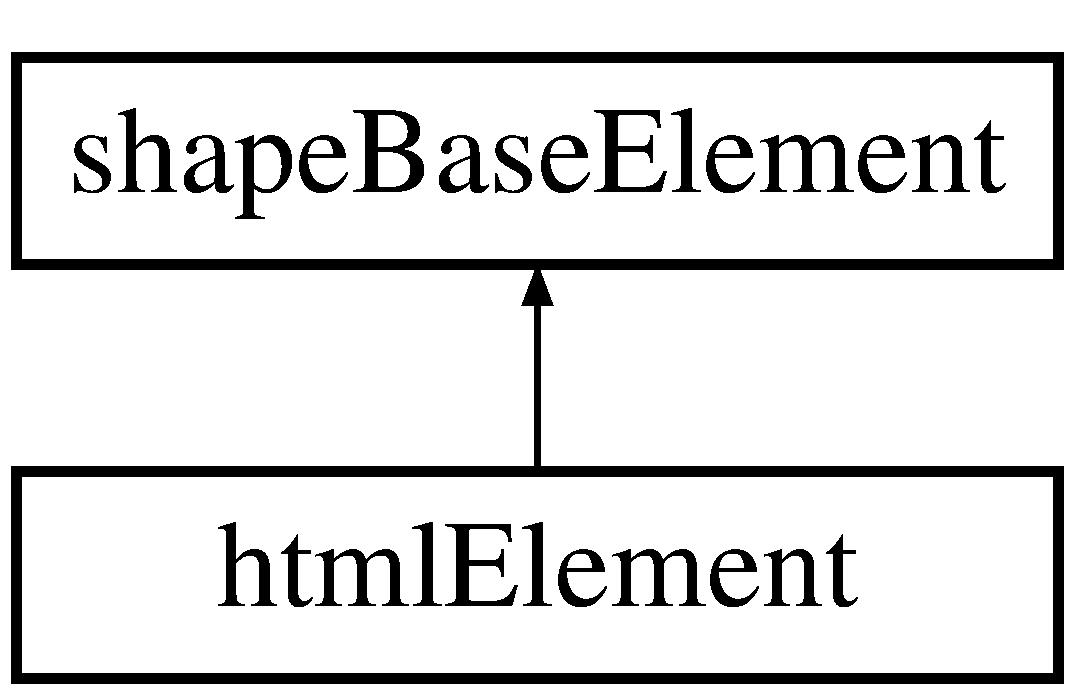
\includegraphics[height=2.000000cm]{classshapeBaseElement}
\end{center}
\end{figure}
\subsection*{Public Member Functions}
\begin{DoxyCompactItemize}
\item 
\hyperlink{classshapeBaseElement_a36980020a9e2e1ab0079b7c6abad349e}{\+\_\+\+\_\+construct} (\$key\+Name=\char`\"{}\char`\"{}, \$key\+Value=\char`\"{}\char`\"{})
\item 
\hyperlink{classshapeBaseElement_af4b541a30cda2b49b6dbf1a3fddec344}{\+\_\+\+\_\+clone} ()
\item 
\hyperlink{classshapeBaseElement_a4547c40cb33c3d34f16a262d1dcca069}{register\+Global} ()
\item 
\hyperlink{classshapeBaseElement_a19aff5da3dce4162e9b6f60226bf1a2c}{get\+Parent} ()
\item 
\hyperlink{classshapeBaseElement_ad6ebb79ad6cb2d501f682938d15d4052}{get\+Value} ()
\item 
\hyperlink{classshapeBaseElement_acc89cd4c440d11f1b771410a096db6c9}{get\+Key} ()
\item 
\hyperlink{classshapeBaseElement_a2ed3481fc7f26976cab34075a9fe7215}{get\+Id} ()
\item 
\hyperlink{classshapeBaseElement_a2549412d8c70edfd3c43d9aa84da49df}{set\+Parent} (\$value=null)
\item 
\hyperlink{classshapeBaseElement_a6353680d2dc0774c53f18050d8bf0df3}{set\+Value} (\$value)
\item 
\hyperlink{classshapeBaseElement_a2d50596a8a0e07ad66401e7c680ec68a}{set\+Key} (\$value)
\item 
\hyperlink{classshapeBaseElement_abbfca908d37f102e4a8e7b353c643d68}{set\+Parent\+Element} (\$parent\+Element)
\item 
\hyperlink{classshapeBaseElement_a091d09076b19adff193a373d3d00b6d8}{get\+Parent\+Element} ()
\end{DoxyCompactItemize}


\subsection{Detailed Description}
The basic shape element class to handle inheritance 

\subsection{Constructor \& Destructor Documentation}
\hypertarget{classshapeBaseElement_a36980020a9e2e1ab0079b7c6abad349e}{}\index{shape\+Base\+Element@{shape\+Base\+Element}!\+\_\+\+\_\+construct@{\+\_\+\+\_\+construct}}
\index{\+\_\+\+\_\+construct@{\+\_\+\+\_\+construct}!shape\+Base\+Element@{shape\+Base\+Element}}
\subsubsection[{\+\_\+\+\_\+construct}]{\setlength{\rightskip}{0pt plus 5cm}shape\+Base\+Element\+::\+\_\+\+\_\+construct (
\begin{DoxyParamCaption}
\item[{}]{\$key\+Name = {\ttfamily \char`\"{}\char`\"{}}, }
\item[{}]{\$key\+Value = {\ttfamily \char`\"{}\char`\"{}}}
\end{DoxyParamCaption}
)}\label{classshapeBaseElement_a36980020a9e2e1ab0079b7c6abad349e}


\subsection{Member Function Documentation}
\hypertarget{classshapeBaseElement_af4b541a30cda2b49b6dbf1a3fddec344}{}\index{shape\+Base\+Element@{shape\+Base\+Element}!\+\_\+\+\_\+clone@{\+\_\+\+\_\+clone}}
\index{\+\_\+\+\_\+clone@{\+\_\+\+\_\+clone}!shape\+Base\+Element@{shape\+Base\+Element}}
\subsubsection[{\+\_\+\+\_\+clone}]{\setlength{\rightskip}{0pt plus 5cm}shape\+Base\+Element\+::\+\_\+\+\_\+clone (
\begin{DoxyParamCaption}
{}
\end{DoxyParamCaption}
)}\label{classshapeBaseElement_af4b541a30cda2b49b6dbf1a3fddec344}
\hypertarget{classshapeBaseElement_a2ed3481fc7f26976cab34075a9fe7215}{}\index{shape\+Base\+Element@{shape\+Base\+Element}!get\+Id@{get\+Id}}
\index{get\+Id@{get\+Id}!shape\+Base\+Element@{shape\+Base\+Element}}
\subsubsection[{get\+Id}]{\setlength{\rightskip}{0pt plus 5cm}shape\+Base\+Element\+::get\+Id (
\begin{DoxyParamCaption}
{}
\end{DoxyParamCaption}
)}\label{classshapeBaseElement_a2ed3481fc7f26976cab34075a9fe7215}
\hypertarget{classshapeBaseElement_acc89cd4c440d11f1b771410a096db6c9}{}\index{shape\+Base\+Element@{shape\+Base\+Element}!get\+Key@{get\+Key}}
\index{get\+Key@{get\+Key}!shape\+Base\+Element@{shape\+Base\+Element}}
\subsubsection[{get\+Key}]{\setlength{\rightskip}{0pt plus 5cm}shape\+Base\+Element\+::get\+Key (
\begin{DoxyParamCaption}
{}
\end{DoxyParamCaption}
)}\label{classshapeBaseElement_acc89cd4c440d11f1b771410a096db6c9}
\hypertarget{classshapeBaseElement_a19aff5da3dce4162e9b6f60226bf1a2c}{}\index{shape\+Base\+Element@{shape\+Base\+Element}!get\+Parent@{get\+Parent}}
\index{get\+Parent@{get\+Parent}!shape\+Base\+Element@{shape\+Base\+Element}}
\subsubsection[{get\+Parent}]{\setlength{\rightskip}{0pt plus 5cm}shape\+Base\+Element\+::get\+Parent (
\begin{DoxyParamCaption}
{}
\end{DoxyParamCaption}
)}\label{classshapeBaseElement_a19aff5da3dce4162e9b6f60226bf1a2c}
\hypertarget{classshapeBaseElement_a091d09076b19adff193a373d3d00b6d8}{}\index{shape\+Base\+Element@{shape\+Base\+Element}!get\+Parent\+Element@{get\+Parent\+Element}}
\index{get\+Parent\+Element@{get\+Parent\+Element}!shape\+Base\+Element@{shape\+Base\+Element}}
\subsubsection[{get\+Parent\+Element}]{\setlength{\rightskip}{0pt plus 5cm}shape\+Base\+Element\+::get\+Parent\+Element (
\begin{DoxyParamCaption}
{}
\end{DoxyParamCaption}
)}\label{classshapeBaseElement_a091d09076b19adff193a373d3d00b6d8}
\hypertarget{classshapeBaseElement_ad6ebb79ad6cb2d501f682938d15d4052}{}\index{shape\+Base\+Element@{shape\+Base\+Element}!get\+Value@{get\+Value}}
\index{get\+Value@{get\+Value}!shape\+Base\+Element@{shape\+Base\+Element}}
\subsubsection[{get\+Value}]{\setlength{\rightskip}{0pt plus 5cm}shape\+Base\+Element\+::get\+Value (
\begin{DoxyParamCaption}
{}
\end{DoxyParamCaption}
)}\label{classshapeBaseElement_ad6ebb79ad6cb2d501f682938d15d4052}
\hypertarget{classshapeBaseElement_a4547c40cb33c3d34f16a262d1dcca069}{}\index{shape\+Base\+Element@{shape\+Base\+Element}!register\+Global@{register\+Global}}
\index{register\+Global@{register\+Global}!shape\+Base\+Element@{shape\+Base\+Element}}
\subsubsection[{register\+Global}]{\setlength{\rightskip}{0pt plus 5cm}shape\+Base\+Element\+::register\+Global (
\begin{DoxyParamCaption}
{}
\end{DoxyParamCaption}
)}\label{classshapeBaseElement_a4547c40cb33c3d34f16a262d1dcca069}
\hypertarget{classshapeBaseElement_a2d50596a8a0e07ad66401e7c680ec68a}{}\index{shape\+Base\+Element@{shape\+Base\+Element}!set\+Key@{set\+Key}}
\index{set\+Key@{set\+Key}!shape\+Base\+Element@{shape\+Base\+Element}}
\subsubsection[{set\+Key}]{\setlength{\rightskip}{0pt plus 5cm}shape\+Base\+Element\+::set\+Key (
\begin{DoxyParamCaption}
\item[{}]{\$value}
\end{DoxyParamCaption}
)}\label{classshapeBaseElement_a2d50596a8a0e07ad66401e7c680ec68a}
\hypertarget{classshapeBaseElement_a2549412d8c70edfd3c43d9aa84da49df}{}\index{shape\+Base\+Element@{shape\+Base\+Element}!set\+Parent@{set\+Parent}}
\index{set\+Parent@{set\+Parent}!shape\+Base\+Element@{shape\+Base\+Element}}
\subsubsection[{set\+Parent}]{\setlength{\rightskip}{0pt plus 5cm}shape\+Base\+Element\+::set\+Parent (
\begin{DoxyParamCaption}
\item[{}]{\$value = {\ttfamily null}}
\end{DoxyParamCaption}
)}\label{classshapeBaseElement_a2549412d8c70edfd3c43d9aa84da49df}
\hypertarget{classshapeBaseElement_abbfca908d37f102e4a8e7b353c643d68}{}\index{shape\+Base\+Element@{shape\+Base\+Element}!set\+Parent\+Element@{set\+Parent\+Element}}
\index{set\+Parent\+Element@{set\+Parent\+Element}!shape\+Base\+Element@{shape\+Base\+Element}}
\subsubsection[{set\+Parent\+Element}]{\setlength{\rightskip}{0pt plus 5cm}shape\+Base\+Element\+::set\+Parent\+Element (
\begin{DoxyParamCaption}
\item[{}]{\$parent\+Element}
\end{DoxyParamCaption}
)}\label{classshapeBaseElement_abbfca908d37f102e4a8e7b353c643d68}
\hypertarget{classshapeBaseElement_a6353680d2dc0774c53f18050d8bf0df3}{}\index{shape\+Base\+Element@{shape\+Base\+Element}!set\+Value@{set\+Value}}
\index{set\+Value@{set\+Value}!shape\+Base\+Element@{shape\+Base\+Element}}
\subsubsection[{set\+Value}]{\setlength{\rightskip}{0pt plus 5cm}shape\+Base\+Element\+::set\+Value (
\begin{DoxyParamCaption}
\item[{}]{\$value}
\end{DoxyParamCaption}
)}\label{classshapeBaseElement_a6353680d2dc0774c53f18050d8bf0df3}


The documentation for this class was generated from the following file\+:\begin{DoxyCompactItemize}
\item 
web\+\_\+root/tina4/\hyperlink{Shape_8php}{Shape.\+php}\end{DoxyCompactItemize}

\hypertarget{classTessa}{}\section{Tessa Class Reference}
\label{classTessa}\index{Tessa@{Tessa}}
\subsection*{Public Member Functions}
\begin{DoxyCompactItemize}
\item 
\hyperlink{classTessa_a27029de5d49d60f83ad7f3afa0db0855}{\+\_\+\+\_\+construct} (\$test\+Dir=\char`\"{}test\char`\"{}, \$browser=\char`\"{}firefox\char`\"{}, \$test\+Server=\char`\"{}\char`\"{})
\item 
\hyperlink{classTessa_a0b42134840fdfef2437c3b2c0c9908b6}{do\+Testing} ()
\item 
\hyperlink{classTessa_a4053ed1b45b0faf76850ee56f2a8578f}{get\+\_\+func\+\_\+arg\+Names} (\$func\+Name)
\item 
\hyperlink{classTessa_a6434d421f09903b7226efba76a050c85}{run\+Tests} ()
\item 
\hyperlink{classTessa_ac4ec71dc20d7f8c1494c56115eeb534d}{\+\_\+\+\_\+call} (\$method, \$args)
\item 
\hyperlink{classTessa_a7e4c039b8228d75810747b96b5062366}{message} (\$msg)
\item 
\hyperlink{classTessa_a54a265707312dd6c5ec290d4877ec05a}{check\+D\+B} (\$tablename, \$fieldname, \$value)
\item 
\hyperlink{classTessa_a54fe80d4ffe3cd047ca3c15e100bbd5c}{fetch\+Records} (\$sql)
\item 
\hyperlink{classTessa_a9e3c7e459e53b5696e8d646d09c05dba}{fetch\+Record} (\$sql)
\item 
\hyperlink{classTessa_ac95db31344f3edd1c2951ce6e0f585db}{trying\+To} (\$msg)
\item 
\hyperlink{classTessa_a9996261064c450e61e6530ec0441b945}{I\+Want\+To} (\$msg)
\item 
\hyperlink{classTessa_aafeac59dfa47fb1501a521bcf9438f15}{add\+Alias} (\$name, \$element)
\item 
\hyperlink{classTessa_a983d3117227db7bf254466936aa8a989}{click\+On} (\$id)
\item 
\hyperlink{classTessa_a1d6ad14ab105a7524cb4f08bfd1d73ca}{look\+For} (\$id)
\item 
\hyperlink{classTessa_a5bf96722ac914ff51e848b14891fb2c0}{get\+Alias} (\$name)
\item 
\hyperlink{classTessa_ae146b22ed7951b61143efd7073d0ea2c}{by\+Id} (\$id)
\item 
\hyperlink{classTessa_a91a3e45138fd2f8325a2a94c4a6ba617}{by\+Path} (\$\hyperlink{Shape_8php_a3b05eec13add53df44e232273d718ae4}{path})
\item 
\hyperlink{classTessa_ac535720770b7bed0ea1120aa121c7ea8}{by\+Class} (\$class)
\item 
\hyperlink{classTessa_af0f1f7c19711f0527bd1372a096038bd}{by\+C\+S\+S} (\$css)
\item 
\hyperlink{classTessa_a71e812fa28e3bdb00c6b2b2ee99cbead}{wait\+For} (\$id)
\item 
\hyperlink{classTessa_a6cc78554f7d5d4a07582b20aed6fcc82}{equals} (\$test1, \$test2)
\item 
\hyperlink{classTessa_a3454246c38eb3976f01d1e9db22cdc4f}{failed} (\$\hyperlink{classTessa_a7e4c039b8228d75810747b96b5062366}{message})
\item 
\hyperlink{classTessa_a410bf71687fffc9d1c5bd674df222eba}{screen\+Shot} ()
\item 
\hyperlink{classTessa_accf6a6c6874c25022b628bc81918a9d0}{Is\+Different} (\$test1, \$test2)
\item 
\hyperlink{classTessa_a98467e5342f835681757cc6d5dfd65ea}{open\+Site} (\$U\+R\+L)
\item 
\hyperlink{classTessa_a97458882c7e72f41358c7991e560be29}{navigate\+To} (\$U\+R\+L)
\item 
\hyperlink{classTessa_ac3a16f8c732b364c4feca92c2f71cc7e}{new\+Session} ()
\item 
\hyperlink{classTessa_a3fce6a71a2303c0bccd0d447375d1c96}{get\+Actions} ()
\item 
\hyperlink{classTessa_ae158939762eb598225ed156a23f95fc2}{delete\+All\+Cookies} ()
\item 
\hyperlink{classTessa_ac6310dd007ead434f3d8cd2698263ded}{accept\+Alert} ()
\item 
\hyperlink{classTessa_a4fbf1f0db39dcb95c2f8c51d73f0b02f}{dismiss\+Alert} ()
\item 
\hyperlink{classTessa_a14a21a710a7eece5d01eb93a010c896e}{execute\+Java\+Script} (\$\hyperlink{Shape_8php_ac2a3056c7a62af99ebe52fdaa4e2e4da}{script}, \$args)
\end{DoxyCompactItemize}


\subsection{Detailed Description}
Class \hyperlink{classTessa}{Tessa} 

\subsection{Constructor \& Destructor Documentation}
\hypertarget{classTessa_a27029de5d49d60f83ad7f3afa0db0855}{}\index{Tessa@{Tessa}!\+\_\+\+\_\+construct@{\+\_\+\+\_\+construct}}
\index{\+\_\+\+\_\+construct@{\+\_\+\+\_\+construct}!Tessa@{Tessa}}
\subsubsection[{\+\_\+\+\_\+construct}]{\setlength{\rightskip}{0pt plus 5cm}Tessa\+::\+\_\+\+\_\+construct (
\begin{DoxyParamCaption}
\item[{}]{\$test\+Dir = {\ttfamily \char`\"{}test\char`\"{}}, }
\item[{}]{\$browser = {\ttfamily \char`\"{}firefox\char`\"{}}, }
\item[{}]{\$test\+Server = {\ttfamily \char`\"{}\char`\"{}}}
\end{DoxyParamCaption}
)}\label{classTessa_a27029de5d49d60f83ad7f3afa0db0855}

\begin{DoxyParams}[1]{Parameters}
string & {\em \$test\+Dir} & \\
\hline
string & {\em \$browser} & \\
\hline
string & {\em \$test\+Server} & \\
\hline
\end{DoxyParams}


\subsection{Member Function Documentation}
\hypertarget{classTessa_ac4ec71dc20d7f8c1494c56115eeb534d}{}\index{Tessa@{Tessa}!\+\_\+\+\_\+call@{\+\_\+\+\_\+call}}
\index{\+\_\+\+\_\+call@{\+\_\+\+\_\+call}!Tessa@{Tessa}}
\subsubsection[{\+\_\+\+\_\+call}]{\setlength{\rightskip}{0pt plus 5cm}Tessa\+::\+\_\+\+\_\+call (
\begin{DoxyParamCaption}
\item[{}]{\$method, }
\item[{}]{\$args}
\end{DoxyParamCaption}
)}\label{classTessa_ac4ec71dc20d7f8c1494c56115eeb534d}

\begin{DoxyParams}{Parameters}
{\em \$method} & \\
\hline
{\em \$args} & \\
\hline
\end{DoxyParams}
\begin{DoxyReturn}{Returns}
mixed 
\end{DoxyReturn}
\hypertarget{classTessa_ac6310dd007ead434f3d8cd2698263ded}{}\index{Tessa@{Tessa}!accept\+Alert@{accept\+Alert}}
\index{accept\+Alert@{accept\+Alert}!Tessa@{Tessa}}
\subsubsection[{accept\+Alert}]{\setlength{\rightskip}{0pt plus 5cm}Tessa\+::accept\+Alert (
\begin{DoxyParamCaption}
{}
\end{DoxyParamCaption}
)}\label{classTessa_ac6310dd007ead434f3d8cd2698263ded}
Accept popup \hypertarget{classTessa_aafeac59dfa47fb1501a521bcf9438f15}{}\index{Tessa@{Tessa}!add\+Alias@{add\+Alias}}
\index{add\+Alias@{add\+Alias}!Tessa@{Tessa}}
\subsubsection[{add\+Alias}]{\setlength{\rightskip}{0pt plus 5cm}Tessa\+::add\+Alias (
\begin{DoxyParamCaption}
\item[{}]{\$name, }
\item[{}]{\$element}
\end{DoxyParamCaption}
)}\label{classTessa_aafeac59dfa47fb1501a521bcf9438f15}

\begin{DoxyParams}{Parameters}
{\em \$name} & \\
\hline
{\em \$element} & \\
\hline
\end{DoxyParams}
\hypertarget{classTessa_ac535720770b7bed0ea1120aa121c7ea8}{}\index{Tessa@{Tessa}!by\+Class@{by\+Class}}
\index{by\+Class@{by\+Class}!Tessa@{Tessa}}
\subsubsection[{by\+Class}]{\setlength{\rightskip}{0pt plus 5cm}Tessa\+::by\+Class (
\begin{DoxyParamCaption}
\item[{}]{\$class}
\end{DoxyParamCaption}
)}\label{classTessa_ac535720770b7bed0ea1120aa121c7ea8}

\begin{DoxyParams}{Parameters}
{\em \$class} & \\
\hline
\end{DoxyParams}
\begin{DoxyReturn}{Returns}
Test\+E\+Lement 
\end{DoxyReturn}
\hypertarget{classTessa_af0f1f7c19711f0527bd1372a096038bd}{}\index{Tessa@{Tessa}!by\+C\+S\+S@{by\+C\+S\+S}}
\index{by\+C\+S\+S@{by\+C\+S\+S}!Tessa@{Tessa}}
\subsubsection[{by\+C\+S\+S}]{\setlength{\rightskip}{0pt plus 5cm}Tessa\+::by\+C\+S\+S (
\begin{DoxyParamCaption}
\item[{}]{\$css}
\end{DoxyParamCaption}
)}\label{classTessa_af0f1f7c19711f0527bd1372a096038bd}

\begin{DoxyParams}{Parameters}
{\em \$css} & \\
\hline
\end{DoxyParams}
\begin{DoxyReturn}{Returns}
Test\+E\+Lement 
\end{DoxyReturn}
\hypertarget{classTessa_ae146b22ed7951b61143efd7073d0ea2c}{}\index{Tessa@{Tessa}!by\+Id@{by\+Id}}
\index{by\+Id@{by\+Id}!Tessa@{Tessa}}
\subsubsection[{by\+Id}]{\setlength{\rightskip}{0pt plus 5cm}Tessa\+::by\+Id (
\begin{DoxyParamCaption}
\item[{}]{\$id}
\end{DoxyParamCaption}
)}\label{classTessa_ae146b22ed7951b61143efd7073d0ea2c}

\begin{DoxyParams}{Parameters}
{\em \$id} & \\
\hline
\end{DoxyParams}
\begin{DoxyReturn}{Returns}
Test\+E\+Lement 
\end{DoxyReturn}
\hypertarget{classTessa_a91a3e45138fd2f8325a2a94c4a6ba617}{}\index{Tessa@{Tessa}!by\+Path@{by\+Path}}
\index{by\+Path@{by\+Path}!Tessa@{Tessa}}
\subsubsection[{by\+Path}]{\setlength{\rightskip}{0pt plus 5cm}Tessa\+::by\+Path (
\begin{DoxyParamCaption}
\item[{}]{\$path}
\end{DoxyParamCaption}
)}\label{classTessa_a91a3e45138fd2f8325a2a94c4a6ba617}

\begin{DoxyParams}{Parameters}
{\em \$path} & \\
\hline
\end{DoxyParams}
\begin{DoxyReturn}{Returns}
Test\+E\+Lement 
\end{DoxyReturn}
\hypertarget{classTessa_a54a265707312dd6c5ec290d4877ec05a}{}\index{Tessa@{Tessa}!check\+D\+B@{check\+D\+B}}
\index{check\+D\+B@{check\+D\+B}!Tessa@{Tessa}}
\subsubsection[{check\+D\+B}]{\setlength{\rightskip}{0pt plus 5cm}Tessa\+::check\+D\+B (
\begin{DoxyParamCaption}
\item[{}]{\$tablename, }
\item[{}]{\$fieldname, }
\item[{}]{\$value}
\end{DoxyParamCaption}
)}\label{classTessa_a54a265707312dd6c5ec290d4877ec05a}
Retrieves a record from the database based on the table, fieldname and value 
\begin{DoxyParams}[1]{Parameters}
String & {\em \$tablename} & The name of the table \\
\hline
String & {\em \$fieldname} & The name of the field \\
\hline
String & {\em \$value} & The expected value \\
\hline
\end{DoxyParams}
\begin{DoxyReturn}{Returns}
Object 
\end{DoxyReturn}
\hypertarget{classTessa_a983d3117227db7bf254466936aa8a989}{}\index{Tessa@{Tessa}!click\+On@{click\+On}}
\index{click\+On@{click\+On}!Tessa@{Tessa}}
\subsubsection[{click\+On}]{\setlength{\rightskip}{0pt plus 5cm}Tessa\+::click\+On (
\begin{DoxyParamCaption}
\item[{}]{\$id}
\end{DoxyParamCaption}
)}\label{classTessa_a983d3117227db7bf254466936aa8a989}

\begin{DoxyParams}{Parameters}
{\em \$id} & \\
\hline
\end{DoxyParams}
\hypertarget{classTessa_ae158939762eb598225ed156a23f95fc2}{}\index{Tessa@{Tessa}!delete\+All\+Cookies@{delete\+All\+Cookies}}
\index{delete\+All\+Cookies@{delete\+All\+Cookies}!Tessa@{Tessa}}
\subsubsection[{delete\+All\+Cookies}]{\setlength{\rightskip}{0pt plus 5cm}Tessa\+::delete\+All\+Cookies (
\begin{DoxyParamCaption}
{}
\end{DoxyParamCaption}
)}\label{classTessa_ae158939762eb598225ed156a23f95fc2}
\hypertarget{classTessa_a4fbf1f0db39dcb95c2f8c51d73f0b02f}{}\index{Tessa@{Tessa}!dismiss\+Alert@{dismiss\+Alert}}
\index{dismiss\+Alert@{dismiss\+Alert}!Tessa@{Tessa}}
\subsubsection[{dismiss\+Alert}]{\setlength{\rightskip}{0pt plus 5cm}Tessa\+::dismiss\+Alert (
\begin{DoxyParamCaption}
{}
\end{DoxyParamCaption}
)}\label{classTessa_a4fbf1f0db39dcb95c2f8c51d73f0b02f}
Dismiss popup \hypertarget{classTessa_a0b42134840fdfef2437c3b2c0c9908b6}{}\index{Tessa@{Tessa}!do\+Testing@{do\+Testing}}
\index{do\+Testing@{do\+Testing}!Tessa@{Tessa}}
\subsubsection[{do\+Testing}]{\setlength{\rightskip}{0pt plus 5cm}Tessa\+::do\+Testing (
\begin{DoxyParamCaption}
{}
\end{DoxyParamCaption}
)}\label{classTessa_a0b42134840fdfef2437c3b2c0c9908b6}
\hypertarget{classTessa_a6cc78554f7d5d4a07582b20aed6fcc82}{}\index{Tessa@{Tessa}!equals@{equals}}
\index{equals@{equals}!Tessa@{Tessa}}
\subsubsection[{equals}]{\setlength{\rightskip}{0pt plus 5cm}Tessa\+::equals (
\begin{DoxyParamCaption}
\item[{}]{\$test1, }
\item[{}]{\$test2}
\end{DoxyParamCaption}
)}\label{classTessa_a6cc78554f7d5d4a07582b20aed6fcc82}

\begin{DoxyParams}{Parameters}
{\em \$test1} & \\
\hline
{\em \$test2} & \\
\hline
\end{DoxyParams}
\hypertarget{classTessa_a14a21a710a7eece5d01eb93a010c896e}{}\index{Tessa@{Tessa}!execute\+Java\+Script@{execute\+Java\+Script}}
\index{execute\+Java\+Script@{execute\+Java\+Script}!Tessa@{Tessa}}
\subsubsection[{execute\+Java\+Script}]{\setlength{\rightskip}{0pt plus 5cm}Tessa\+::execute\+Java\+Script (
\begin{DoxyParamCaption}
\item[{}]{\$script, }
\item[{}]{\$args}
\end{DoxyParamCaption}
)}\label{classTessa_a14a21a710a7eece5d01eb93a010c896e}
Execute J\+S \hypertarget{classTessa_a3454246c38eb3976f01d1e9db22cdc4f}{}\index{Tessa@{Tessa}!failed@{failed}}
\index{failed@{failed}!Tessa@{Tessa}}
\subsubsection[{failed}]{\setlength{\rightskip}{0pt plus 5cm}Tessa\+::failed (
\begin{DoxyParamCaption}
\item[{}]{\$message}
\end{DoxyParamCaption}
)}\label{classTessa_a3454246c38eb3976f01d1e9db22cdc4f}

\begin{DoxyParams}{Parameters}
{\em \$message} & \\
\hline
\end{DoxyParams}
\hypertarget{classTessa_a9e3c7e459e53b5696e8d646d09c05dba}{}\index{Tessa@{Tessa}!fetch\+Record@{fetch\+Record}}
\index{fetch\+Record@{fetch\+Record}!Tessa@{Tessa}}
\subsubsection[{fetch\+Record}]{\setlength{\rightskip}{0pt plus 5cm}Tessa\+::fetch\+Record (
\begin{DoxyParamCaption}
\item[{}]{\$sql}
\end{DoxyParamCaption}
)}\label{classTessa_a9e3c7e459e53b5696e8d646d09c05dba}
Function to retrieve a record from the database 
\begin{DoxyParams}[1]{Parameters}
String & {\em \$sql} & \\
\hline
\end{DoxyParams}
\begin{DoxyReturn}{Returns}
Object 
\end{DoxyReturn}
\hypertarget{classTessa_a54fe80d4ffe3cd047ca3c15e100bbd5c}{}\index{Tessa@{Tessa}!fetch\+Records@{fetch\+Records}}
\index{fetch\+Records@{fetch\+Records}!Tessa@{Tessa}}
\subsubsection[{fetch\+Records}]{\setlength{\rightskip}{0pt plus 5cm}Tessa\+::fetch\+Records (
\begin{DoxyParamCaption}
\item[{}]{\$sql}
\end{DoxyParamCaption}
)}\label{classTessa_a54fe80d4ffe3cd047ca3c15e100bbd5c}
Function to retrieve records from the database 
\begin{DoxyParams}[1]{Parameters}
String & {\em \$sql} & \\
\hline
\end{DoxyParams}
\begin{DoxyReturn}{Returns}
Object 
\end{DoxyReturn}
\hypertarget{classTessa_a4053ed1b45b0faf76850ee56f2a8578f}{}\index{Tessa@{Tessa}!get\+\_\+func\+\_\+arg\+Names@{get\+\_\+func\+\_\+arg\+Names}}
\index{get\+\_\+func\+\_\+arg\+Names@{get\+\_\+func\+\_\+arg\+Names}!Tessa@{Tessa}}
\subsubsection[{get\+\_\+func\+\_\+arg\+Names}]{\setlength{\rightskip}{0pt plus 5cm}Tessa\+::get\+\_\+func\+\_\+arg\+Names (
\begin{DoxyParamCaption}
\item[{}]{\$func\+Name}
\end{DoxyParamCaption}
)}\label{classTessa_a4053ed1b45b0faf76850ee56f2a8578f}

\begin{DoxyParams}{Parameters}
{\em \$func\+Name} & \\
\hline
\end{DoxyParams}
\begin{DoxyReturn}{Returns}
array 
\end{DoxyReturn}
\hypertarget{classTessa_a3fce6a71a2303c0bccd0d447375d1c96}{}\index{Tessa@{Tessa}!get\+Actions@{get\+Actions}}
\index{get\+Actions@{get\+Actions}!Tessa@{Tessa}}
\subsubsection[{get\+Actions}]{\setlength{\rightskip}{0pt plus 5cm}Tessa\+::get\+Actions (
\begin{DoxyParamCaption}
{}
\end{DoxyParamCaption}
)}\label{classTessa_a3fce6a71a2303c0bccd0d447375d1c96}
\begin{DoxyReturn}{Returns}
P\+H\+P\+Web\+Driver\+\_\+\+Web\+Driver\+Action\+Chains 
\end{DoxyReturn}
\hypertarget{classTessa_a5bf96722ac914ff51e848b14891fb2c0}{}\index{Tessa@{Tessa}!get\+Alias@{get\+Alias}}
\index{get\+Alias@{get\+Alias}!Tessa@{Tessa}}
\subsubsection[{get\+Alias}]{\setlength{\rightskip}{0pt plus 5cm}Tessa\+::get\+Alias (
\begin{DoxyParamCaption}
\item[{}]{\$name}
\end{DoxyParamCaption}
)}\label{classTessa_a5bf96722ac914ff51e848b14891fb2c0}

\begin{DoxyParams}{Parameters}
{\em \$name} & \\
\hline
\end{DoxyParams}
\begin{DoxyReturn}{Returns}
null 
\end{DoxyReturn}
\hypertarget{classTessa_accf6a6c6874c25022b628bc81918a9d0}{}\index{Tessa@{Tessa}!Is\+Different@{Is\+Different}}
\index{Is\+Different@{Is\+Different}!Tessa@{Tessa}}
\subsubsection[{Is\+Different}]{\setlength{\rightskip}{0pt plus 5cm}Tessa\+::\+Is\+Different (
\begin{DoxyParamCaption}
\item[{}]{\$test1, }
\item[{}]{\$test2}
\end{DoxyParamCaption}
)}\label{classTessa_accf6a6c6874c25022b628bc81918a9d0}
Reuben --- Check if two test cases are different 
\begin{DoxyParams}{Parameters}
{\em \$test1} & \\
\hline
{\em \$test2} & \\
\hline
\end{DoxyParams}
\hypertarget{classTessa_a9996261064c450e61e6530ec0441b945}{}\index{Tessa@{Tessa}!I\+Want\+To@{I\+Want\+To}}
\index{I\+Want\+To@{I\+Want\+To}!Tessa@{Tessa}}
\subsubsection[{I\+Want\+To}]{\setlength{\rightskip}{0pt plus 5cm}Tessa\+::\+I\+Want\+To (
\begin{DoxyParamCaption}
\item[{}]{\$msg}
\end{DoxyParamCaption}
)}\label{classTessa_a9996261064c450e61e6530ec0441b945}
Display a message on the screen prefixed with I want to 
\begin{DoxyParams}{Parameters}
{\em \$msg} & \\
\hline
\end{DoxyParams}
\hypertarget{classTessa_a1d6ad14ab105a7524cb4f08bfd1d73ca}{}\index{Tessa@{Tessa}!look\+For@{look\+For}}
\index{look\+For@{look\+For}!Tessa@{Tessa}}
\subsubsection[{look\+For}]{\setlength{\rightskip}{0pt plus 5cm}Tessa\+::look\+For (
\begin{DoxyParamCaption}
\item[{}]{\$id}
\end{DoxyParamCaption}
)}\label{classTessa_a1d6ad14ab105a7524cb4f08bfd1d73ca}

\begin{DoxyParams}{Parameters}
{\em \$id} & \\
\hline
\end{DoxyParams}
\begin{DoxyReturn}{Returns}
null$\vert$\+Test\+E\+Lement 
\end{DoxyReturn}
\hypertarget{classTessa_a7e4c039b8228d75810747b96b5062366}{}\index{Tessa@{Tessa}!message@{message}}
\index{message@{message}!Tessa@{Tessa}}
\subsubsection[{message}]{\setlength{\rightskip}{0pt plus 5cm}Tessa\+::message (
\begin{DoxyParamCaption}
\item[{}]{\$msg}
\end{DoxyParamCaption}
)}\label{classTessa_a7e4c039b8228d75810747b96b5062366}
Display a message on the screen 
\begin{DoxyParams}{Parameters}
{\em \$msg} & \\
\hline
\end{DoxyParams}
\hypertarget{classTessa_a97458882c7e72f41358c7991e560be29}{}\index{Tessa@{Tessa}!navigate\+To@{navigate\+To}}
\index{navigate\+To@{navigate\+To}!Tessa@{Tessa}}
\subsubsection[{navigate\+To}]{\setlength{\rightskip}{0pt plus 5cm}Tessa\+::navigate\+To (
\begin{DoxyParamCaption}
\item[{}]{\$\+U\+R\+L}
\end{DoxyParamCaption}
)}\label{classTessa_a97458882c7e72f41358c7991e560be29}

\begin{DoxyParams}{Parameters}
{\em \$\+U\+R\+L} & \\
\hline
\end{DoxyParams}
\begin{DoxyReturn}{Returns}
bool 
\end{DoxyReturn}
\hypertarget{classTessa_ac3a16f8c732b364c4feca92c2f71cc7e}{}\index{Tessa@{Tessa}!new\+Session@{new\+Session}}
\index{new\+Session@{new\+Session}!Tessa@{Tessa}}
\subsubsection[{new\+Session}]{\setlength{\rightskip}{0pt plus 5cm}Tessa\+::new\+Session (
\begin{DoxyParamCaption}
{}
\end{DoxyParamCaption}
)}\label{classTessa_ac3a16f8c732b364c4feca92c2f71cc7e}
\hypertarget{classTessa_a98467e5342f835681757cc6d5dfd65ea}{}\index{Tessa@{Tessa}!open\+Site@{open\+Site}}
\index{open\+Site@{open\+Site}!Tessa@{Tessa}}
\subsubsection[{open\+Site}]{\setlength{\rightskip}{0pt plus 5cm}Tessa\+::open\+Site (
\begin{DoxyParamCaption}
\item[{}]{\$\+U\+R\+L}
\end{DoxyParamCaption}
)}\label{classTessa_a98467e5342f835681757cc6d5dfd65ea}

\begin{DoxyParams}{Parameters}
{\em \$\+U\+R\+L} & \\
\hline
\end{DoxyParams}
\begin{DoxyReturn}{Returns}
bool 
\end{DoxyReturn}
\hypertarget{classTessa_a6434d421f09903b7226efba76a050c85}{}\index{Tessa@{Tessa}!run\+Tests@{run\+Tests}}
\index{run\+Tests@{run\+Tests}!Tessa@{Tessa}}
\subsubsection[{run\+Tests}]{\setlength{\rightskip}{0pt plus 5cm}Tessa\+::run\+Tests (
\begin{DoxyParamCaption}
{}
\end{DoxyParamCaption}
)}\label{classTessa_a6434d421f09903b7226efba76a050c85}
\hypertarget{classTessa_a410bf71687fffc9d1c5bd674df222eba}{}\index{Tessa@{Tessa}!screen\+Shot@{screen\+Shot}}
\index{screen\+Shot@{screen\+Shot}!Tessa@{Tessa}}
\subsubsection[{screen\+Shot}]{\setlength{\rightskip}{0pt plus 5cm}Tessa\+::screen\+Shot (
\begin{DoxyParamCaption}
{}
\end{DoxyParamCaption}
)}\label{classTessa_a410bf71687fffc9d1c5bd674df222eba}
A function to create screenshots when something fails \begin{DoxyReturn}{Returns}
String The H\+T\+M\+L path to the screen shot 
\end{DoxyReturn}
\hypertarget{classTessa_ac95db31344f3edd1c2951ce6e0f585db}{}\index{Tessa@{Tessa}!trying\+To@{trying\+To}}
\index{trying\+To@{trying\+To}!Tessa@{Tessa}}
\subsubsection[{trying\+To}]{\setlength{\rightskip}{0pt plus 5cm}Tessa\+::trying\+To (
\begin{DoxyParamCaption}
\item[{}]{\$msg}
\end{DoxyParamCaption}
)}\label{classTessa_ac95db31344f3edd1c2951ce6e0f585db}
Display a message on the screen prefixed with Trying to 
\begin{DoxyParams}{Parameters}
{\em \$msg} & \\
\hline
\end{DoxyParams}
\hypertarget{classTessa_a71e812fa28e3bdb00c6b2b2ee99cbead}{}\index{Tessa@{Tessa}!wait\+For@{wait\+For}}
\index{wait\+For@{wait\+For}!Tessa@{Tessa}}
\subsubsection[{wait\+For}]{\setlength{\rightskip}{0pt plus 5cm}Tessa\+::wait\+For (
\begin{DoxyParamCaption}
\item[{}]{\$id}
\end{DoxyParamCaption}
)}\label{classTessa_a71e812fa28e3bdb00c6b2b2ee99cbead}

\begin{DoxyParams}{Parameters}
{\em \$id} & \\
\hline
\end{DoxyParams}
\begin{DoxyReturn}{Returns}
Test\+E\+Lement 
\end{DoxyReturn}


The documentation for this class was generated from the following file\+:\begin{DoxyCompactItemize}
\item 
web\+\_\+root/tina4/\hyperlink{Tessa_8php}{Tessa.\+php}\end{DoxyCompactItemize}

\hypertarget{classtestClass}{}\section{test\+Class Class Reference}
\label{classtestClass}\index{test\+Class@{test\+Class}}
\subsection*{Public Member Functions}
\begin{DoxyCompactItemize}
\item 
\hyperlink{classtestClass_a1e158e86f9bf4fc8c4f04d32fef8d079}{get\+Display} (\$name=\char`\"{}World\char`\"{}, \$age=10)
\item 
\hyperlink{classtestClass_a189a8246c78c5da4d5f49685349ae070}{get\+Names} ()
\item 
\hyperlink{classtestClass_a27e1098ad521d47aa53d15a2f862da30}{get\+Pets} (\$user\+Id=0)
\end{DoxyCompactItemize}


\subsection{Member Function Documentation}
\hypertarget{classtestClass_a1e158e86f9bf4fc8c4f04d32fef8d079}{}\index{test\+Class@{test\+Class}!get\+Display@{get\+Display}}
\index{get\+Display@{get\+Display}!test\+Class@{test\+Class}}
\subsubsection[{get\+Display}]{\setlength{\rightskip}{0pt plus 5cm}test\+Class\+::get\+Display (
\begin{DoxyParamCaption}
\item[{}]{\$name = {\ttfamily \char`\"{}World\char`\"{}}, }
\item[{}]{\$age = {\ttfamily 10}}
\end{DoxyParamCaption}
)}\label{classtestClass_a1e158e86f9bf4fc8c4f04d32fef8d079}
\hypertarget{classtestClass_a189a8246c78c5da4d5f49685349ae070}{}\index{test\+Class@{test\+Class}!get\+Names@{get\+Names}}
\index{get\+Names@{get\+Names}!test\+Class@{test\+Class}}
\subsubsection[{get\+Names}]{\setlength{\rightskip}{0pt plus 5cm}test\+Class\+::get\+Names (
\begin{DoxyParamCaption}
{}
\end{DoxyParamCaption}
)}\label{classtestClass_a189a8246c78c5da4d5f49685349ae070}
\hypertarget{classtestClass_a27e1098ad521d47aa53d15a2f862da30}{}\index{test\+Class@{test\+Class}!get\+Pets@{get\+Pets}}
\index{get\+Pets@{get\+Pets}!test\+Class@{test\+Class}}
\subsubsection[{get\+Pets}]{\setlength{\rightskip}{0pt plus 5cm}test\+Class\+::get\+Pets (
\begin{DoxyParamCaption}
\item[{}]{\$user\+Id = {\ttfamily 0}}
\end{DoxyParamCaption}
)}\label{classtestClass_a27e1098ad521d47aa53d15a2f862da30}


The documentation for this class was generated from the following file\+:\begin{DoxyCompactItemize}
\item 
web\+\_\+root/project/\hyperlink{testClass_8php}{test\+Class.\+php}\end{DoxyCompactItemize}

\hypertarget{classTestElement}{}\section{Test\+Element Class Reference}
\label{classTestElement}\index{Test\+Element@{Test\+Element}}
\subsection*{Public Member Functions}
\begin{DoxyCompactItemize}
\item 
\hyperlink{classTestElement_a5555f24285021a20747175e5fa686fbf}{\+\_\+\+\_\+construct} (\$element)
\item 
\hyperlink{classTestElement_ac3025f8014dade5d754d3943689a396f}{by\+Path} (\$\hyperlink{Shape_8php_a3b05eec13add53df44e232273d718ae4}{path})
\item 
\hyperlink{classTestElement_a584de1c2c8c24eb790f493102bcb1fac}{by\+Id} (\$id)
\item 
\hyperlink{classTestElement_a46f9075b924f047895d576e0af82d9c9}{by\+Tag} (\$tag)
\item 
\hyperlink{classTestElement_a56ad09c49ee8c9781b8c50ab31d08b22}{choose\+Option} (\$value)
\item 
\hyperlink{classTestElement_aaf0f757cf4dfc5925d0db204bcb252d5}{by\+C\+S\+S} (\$css)
\item 
\hyperlink{classTestElement_a5211d65c1aa197f6dc1e22e24283abb2}{by\+Class} (\$class)
\item 
\hyperlink{classTestElement_a37b4de38664b658faa86ade0d7073dd4}{and\+Set\+Text} (\$\hyperlink{Shape_8php_a37df362c2f77a0045fa8af094f432238}{text})
\item 
\hyperlink{classTestElement_ac5968c56cb813dba50a15b50946e5330}{set\+Text} (\$\hyperlink{Shape_8php_a37df362c2f77a0045fa8af094f432238}{text}, \$clear=\hyperlink{tina4_8php_aec2deb5590a84bee262c3bea206ae88f}{false})
\item 
\hyperlink{classTestElement_a7f2722947e83c9268799ab59294626bc}{and\+Add\+Text} (\$\hyperlink{Shape_8php_a37df362c2f77a0045fa8af094f432238}{text})
\item 
\hyperlink{classTestElement_a86c3a50de5a568d5ca9a75339ef1a417}{get\+Text} ()
\item 
\hyperlink{classTestElement_a1964043ed9be26b977b5ed6b4d993aaa}{get\+Value} ()
\item 
\hyperlink{classTestElement_ad9fd0dc7b25f15c78483e0710dea2d04}{get\+Attr} (\$attr)
\item 
\hyperlink{classTestElement_ae61d3f666ac5c098dec914bcb7fdeaf6}{set\+Value} (\$value)
\item 
\hyperlink{classTestElement_af4d9e324bfc49d733cfadc4825da425c}{and\+Click} ()
\item 
\hyperlink{classTestElement_aa32acc6f9604f1fff02ecb37197627b3}{click} ()
\item 
\hyperlink{classTestElement_a05bb2b21ee3bd09a24a04e879c079d95}{and\+Alias} (\$name)
\item 
\hyperlink{classTestElement_adb5c0bdaa41a4e52f65f927d425b802e}{drag\+And\+Drop} (\$target, \$options)
\item 
\hyperlink{classTestElement_a6fe91b896213fbe4185a85ba450cd571}{click\+And\+Hold} ()
\item 
\hyperlink{classTestElement_a2b6ab197b32c1eb95759f3576e7f5254}{get\+I\+D} ()
\end{DoxyCompactItemize}


\subsection{Detailed Description}
Test Element used by \hyperlink{classTessa}{Tessa} 

\subsection{Constructor \& Destructor Documentation}
\hypertarget{classTestElement_a5555f24285021a20747175e5fa686fbf}{}\index{Test\+Element@{Test\+Element}!\+\_\+\+\_\+construct@{\+\_\+\+\_\+construct}}
\index{\+\_\+\+\_\+construct@{\+\_\+\+\_\+construct}!Test\+Element@{Test\+Element}}
\subsubsection[{\+\_\+\+\_\+construct}]{\setlength{\rightskip}{0pt plus 5cm}Test\+Element\+::\+\_\+\+\_\+construct (
\begin{DoxyParamCaption}
\item[{}]{\$element}
\end{DoxyParamCaption}
)}\label{classTestElement_a5555f24285021a20747175e5fa686fbf}

\begin{DoxyParams}{Parameters}
{\em \$element} & \\
\hline
\end{DoxyParams}


\subsection{Member Function Documentation}
\hypertarget{classTestElement_a7f2722947e83c9268799ab59294626bc}{}\index{Test\+Element@{Test\+Element}!and\+Add\+Text@{and\+Add\+Text}}
\index{and\+Add\+Text@{and\+Add\+Text}!Test\+Element@{Test\+Element}}
\subsubsection[{and\+Add\+Text}]{\setlength{\rightskip}{0pt plus 5cm}Test\+Element\+::and\+Add\+Text (
\begin{DoxyParamCaption}
\item[{}]{\$text}
\end{DoxyParamCaption}
)}\label{classTestElement_a7f2722947e83c9268799ab59294626bc}

\begin{DoxyParams}{Parameters}
{\em \$text} & \\
\hline
\end{DoxyParams}
\hypertarget{classTestElement_a05bb2b21ee3bd09a24a04e879c079d95}{}\index{Test\+Element@{Test\+Element}!and\+Alias@{and\+Alias}}
\index{and\+Alias@{and\+Alias}!Test\+Element@{Test\+Element}}
\subsubsection[{and\+Alias}]{\setlength{\rightskip}{0pt plus 5cm}Test\+Element\+::and\+Alias (
\begin{DoxyParamCaption}
\item[{}]{\$name}
\end{DoxyParamCaption}
)}\label{classTestElement_a05bb2b21ee3bd09a24a04e879c079d95}

\begin{DoxyParams}{Parameters}
{\em \$name} & \\
\hline
\end{DoxyParams}
\begin{DoxyReturn}{Returns}
mixed 
\end{DoxyReturn}
\hypertarget{classTestElement_af4d9e324bfc49d733cfadc4825da425c}{}\index{Test\+Element@{Test\+Element}!and\+Click@{and\+Click}}
\index{and\+Click@{and\+Click}!Test\+Element@{Test\+Element}}
\subsubsection[{and\+Click}]{\setlength{\rightskip}{0pt plus 5cm}Test\+Element\+::and\+Click (
\begin{DoxyParamCaption}
{}
\end{DoxyParamCaption}
)}\label{classTestElement_af4d9e324bfc49d733cfadc4825da425c}
\hypertarget{classTestElement_a37b4de38664b658faa86ade0d7073dd4}{}\index{Test\+Element@{Test\+Element}!and\+Set\+Text@{and\+Set\+Text}}
\index{and\+Set\+Text@{and\+Set\+Text}!Test\+Element@{Test\+Element}}
\subsubsection[{and\+Set\+Text}]{\setlength{\rightskip}{0pt plus 5cm}Test\+Element\+::and\+Set\+Text (
\begin{DoxyParamCaption}
\item[{}]{\$text}
\end{DoxyParamCaption}
)}\label{classTestElement_a37b4de38664b658faa86ade0d7073dd4}

\begin{DoxyParams}{Parameters}
{\em \$text} & \\
\hline
\end{DoxyParams}
\hypertarget{classTestElement_a5211d65c1aa197f6dc1e22e24283abb2}{}\index{Test\+Element@{Test\+Element}!by\+Class@{by\+Class}}
\index{by\+Class@{by\+Class}!Test\+Element@{Test\+Element}}
\subsubsection[{by\+Class}]{\setlength{\rightskip}{0pt plus 5cm}Test\+Element\+::by\+Class (
\begin{DoxyParamCaption}
\item[{}]{\$class}
\end{DoxyParamCaption}
)}\label{classTestElement_a5211d65c1aa197f6dc1e22e24283abb2}

\begin{DoxyParams}{Parameters}
{\em \$class} & \\
\hline
\end{DoxyParams}
\begin{DoxyReturn}{Returns}
\hyperlink{classTestElement}{Test\+Element} 
\end{DoxyReturn}
\hypertarget{classTestElement_aaf0f757cf4dfc5925d0db204bcb252d5}{}\index{Test\+Element@{Test\+Element}!by\+C\+S\+S@{by\+C\+S\+S}}
\index{by\+C\+S\+S@{by\+C\+S\+S}!Test\+Element@{Test\+Element}}
\subsubsection[{by\+C\+S\+S}]{\setlength{\rightskip}{0pt plus 5cm}Test\+Element\+::by\+C\+S\+S (
\begin{DoxyParamCaption}
\item[{}]{\$css}
\end{DoxyParamCaption}
)}\label{classTestElement_aaf0f757cf4dfc5925d0db204bcb252d5}

\begin{DoxyParams}{Parameters}
{\em \$css} & \\
\hline
\end{DoxyParams}
\begin{DoxyReturn}{Returns}
Test\+E\+Lement 
\end{DoxyReturn}
\hypertarget{classTestElement_a584de1c2c8c24eb790f493102bcb1fac}{}\index{Test\+Element@{Test\+Element}!by\+Id@{by\+Id}}
\index{by\+Id@{by\+Id}!Test\+Element@{Test\+Element}}
\subsubsection[{by\+Id}]{\setlength{\rightskip}{0pt plus 5cm}Test\+Element\+::by\+Id (
\begin{DoxyParamCaption}
\item[{}]{\$id}
\end{DoxyParamCaption}
)}\label{classTestElement_a584de1c2c8c24eb790f493102bcb1fac}

\begin{DoxyParams}{Parameters}
{\em \$id} & \\
\hline
\end{DoxyParams}
\begin{DoxyReturn}{Returns}
\hyperlink{classTestElement}{Test\+Element} 
\end{DoxyReturn}
\hypertarget{classTestElement_ac3025f8014dade5d754d3943689a396f}{}\index{Test\+Element@{Test\+Element}!by\+Path@{by\+Path}}
\index{by\+Path@{by\+Path}!Test\+Element@{Test\+Element}}
\subsubsection[{by\+Path}]{\setlength{\rightskip}{0pt plus 5cm}Test\+Element\+::by\+Path (
\begin{DoxyParamCaption}
\item[{}]{\$path}
\end{DoxyParamCaption}
)}\label{classTestElement_ac3025f8014dade5d754d3943689a396f}

\begin{DoxyParams}{Parameters}
{\em \$path} & \\
\hline
\end{DoxyParams}
\begin{DoxyReturn}{Returns}
\hyperlink{classTestElement}{Test\+Element} 
\end{DoxyReturn}
\hypertarget{classTestElement_a46f9075b924f047895d576e0af82d9c9}{}\index{Test\+Element@{Test\+Element}!by\+Tag@{by\+Tag}}
\index{by\+Tag@{by\+Tag}!Test\+Element@{Test\+Element}}
\subsubsection[{by\+Tag}]{\setlength{\rightskip}{0pt plus 5cm}Test\+Element\+::by\+Tag (
\begin{DoxyParamCaption}
\item[{}]{\$tag}
\end{DoxyParamCaption}
)}\label{classTestElement_a46f9075b924f047895d576e0af82d9c9}

\begin{DoxyParams}{Parameters}
{\em \$tag} & \\
\hline
\end{DoxyParams}
\begin{DoxyReturn}{Returns}
Test\+E\+Lement 
\end{DoxyReturn}
\hypertarget{classTestElement_a56ad09c49ee8c9781b8c50ab31d08b22}{}\index{Test\+Element@{Test\+Element}!choose\+Option@{choose\+Option}}
\index{choose\+Option@{choose\+Option}!Test\+Element@{Test\+Element}}
\subsubsection[{choose\+Option}]{\setlength{\rightskip}{0pt plus 5cm}Test\+Element\+::choose\+Option (
\begin{DoxyParamCaption}
\item[{}]{\$value}
\end{DoxyParamCaption}
)}\label{classTestElement_a56ad09c49ee8c9781b8c50ab31d08b22}

\begin{DoxyParams}{Parameters}
{\em \$value} & \\
\hline
\end{DoxyParams}
\begin{DoxyReturn}{Returns}
\hyperlink{classTestElement}{Test\+Element} 
\end{DoxyReturn}
\hypertarget{classTestElement_aa32acc6f9604f1fff02ecb37197627b3}{}\index{Test\+Element@{Test\+Element}!click@{click}}
\index{click@{click}!Test\+Element@{Test\+Element}}
\subsubsection[{click}]{\setlength{\rightskip}{0pt plus 5cm}Test\+Element\+::click (
\begin{DoxyParamCaption}
{}
\end{DoxyParamCaption}
)}\label{classTestElement_aa32acc6f9604f1fff02ecb37197627b3}
\hypertarget{classTestElement_a6fe91b896213fbe4185a85ba450cd571}{}\index{Test\+Element@{Test\+Element}!click\+And\+Hold@{click\+And\+Hold}}
\index{click\+And\+Hold@{click\+And\+Hold}!Test\+Element@{Test\+Element}}
\subsubsection[{click\+And\+Hold}]{\setlength{\rightskip}{0pt plus 5cm}Test\+Element\+::click\+And\+Hold (
\begin{DoxyParamCaption}
{}
\end{DoxyParamCaption}
)}\label{classTestElement_a6fe91b896213fbe4185a85ba450cd571}
\hypertarget{classTestElement_adb5c0bdaa41a4e52f65f927d425b802e}{}\index{Test\+Element@{Test\+Element}!drag\+And\+Drop@{drag\+And\+Drop}}
\index{drag\+And\+Drop@{drag\+And\+Drop}!Test\+Element@{Test\+Element}}
\subsubsection[{drag\+And\+Drop}]{\setlength{\rightskip}{0pt plus 5cm}Test\+Element\+::drag\+And\+Drop (
\begin{DoxyParamCaption}
\item[{}]{\$target, }
\item[{}]{\$options}
\end{DoxyParamCaption}
)}\label{classTestElement_adb5c0bdaa41a4e52f65f927d425b802e}

\begin{DoxyParams}{Parameters}
{\em \$target} & \\
\hline
{\em \$options} & \\
\hline
\end{DoxyParams}
\hypertarget{classTestElement_ad9fd0dc7b25f15c78483e0710dea2d04}{}\index{Test\+Element@{Test\+Element}!get\+Attr@{get\+Attr}}
\index{get\+Attr@{get\+Attr}!Test\+Element@{Test\+Element}}
\subsubsection[{get\+Attr}]{\setlength{\rightskip}{0pt plus 5cm}Test\+Element\+::get\+Attr (
\begin{DoxyParamCaption}
\item[{}]{\$attr}
\end{DoxyParamCaption}
)}\label{classTestElement_ad9fd0dc7b25f15c78483e0710dea2d04}

\begin{DoxyParams}{Parameters}
{\em \$attr} & \\
\hline
\end{DoxyParams}
\begin{DoxyReturn}{Returns}
mixed 
\end{DoxyReturn}
\hypertarget{classTestElement_a2b6ab197b32c1eb95759f3576e7f5254}{}\index{Test\+Element@{Test\+Element}!get\+I\+D@{get\+I\+D}}
\index{get\+I\+D@{get\+I\+D}!Test\+Element@{Test\+Element}}
\subsubsection[{get\+I\+D}]{\setlength{\rightskip}{0pt plus 5cm}Test\+Element\+::get\+I\+D (
\begin{DoxyParamCaption}
{}
\end{DoxyParamCaption}
)}\label{classTestElement_a2b6ab197b32c1eb95759f3576e7f5254}
\begin{DoxyReturn}{Returns}
mixed 
\end{DoxyReturn}
\hypertarget{classTestElement_a86c3a50de5a568d5ca9a75339ef1a417}{}\index{Test\+Element@{Test\+Element}!get\+Text@{get\+Text}}
\index{get\+Text@{get\+Text}!Test\+Element@{Test\+Element}}
\subsubsection[{get\+Text}]{\setlength{\rightskip}{0pt plus 5cm}Test\+Element\+::get\+Text (
\begin{DoxyParamCaption}
{}
\end{DoxyParamCaption}
)}\label{classTestElement_a86c3a50de5a568d5ca9a75339ef1a417}
\begin{DoxyReturn}{Returns}
mixed 
\end{DoxyReturn}
\hypertarget{classTestElement_a1964043ed9be26b977b5ed6b4d993aaa}{}\index{Test\+Element@{Test\+Element}!get\+Value@{get\+Value}}
\index{get\+Value@{get\+Value}!Test\+Element@{Test\+Element}}
\subsubsection[{get\+Value}]{\setlength{\rightskip}{0pt plus 5cm}Test\+Element\+::get\+Value (
\begin{DoxyParamCaption}
{}
\end{DoxyParamCaption}
)}\label{classTestElement_a1964043ed9be26b977b5ed6b4d993aaa}
\begin{DoxyReturn}{Returns}
mixed 
\end{DoxyReturn}
\hypertarget{classTestElement_ac5968c56cb813dba50a15b50946e5330}{}\index{Test\+Element@{Test\+Element}!set\+Text@{set\+Text}}
\index{set\+Text@{set\+Text}!Test\+Element@{Test\+Element}}
\subsubsection[{set\+Text}]{\setlength{\rightskip}{0pt plus 5cm}Test\+Element\+::set\+Text (
\begin{DoxyParamCaption}
\item[{}]{\$text, }
\item[{}]{\$clear = {\ttfamily {\bf false}}}
\end{DoxyParamCaption}
)}\label{classTestElement_ac5968c56cb813dba50a15b50946e5330}

\begin{DoxyParams}[1]{Parameters}
 & {\em \$text} & \\
\hline
bool & {\em \$clear} & \\
\hline
\end{DoxyParams}
\hypertarget{classTestElement_ae61d3f666ac5c098dec914bcb7fdeaf6}{}\index{Test\+Element@{Test\+Element}!set\+Value@{set\+Value}}
\index{set\+Value@{set\+Value}!Test\+Element@{Test\+Element}}
\subsubsection[{set\+Value}]{\setlength{\rightskip}{0pt plus 5cm}Test\+Element\+::set\+Value (
\begin{DoxyParamCaption}
\item[{}]{\$value}
\end{DoxyParamCaption}
)}\label{classTestElement_ae61d3f666ac5c098dec914bcb7fdeaf6}

\begin{DoxyParams}{Parameters}
{\em \$value} & \\
\hline
\end{DoxyParams}


The documentation for this class was generated from the following file\+:\begin{DoxyCompactItemize}
\item 
web\+\_\+root/tina4/\hyperlink{Tessa_8php}{Tessa.\+php}\end{DoxyCompactItemize}

\chapter{File Documentation}
\hypertarget{testClass_8php}{}\section{web\+\_\+root/project/test\+Class.php File Reference}
\label{testClass_8php}\index{web\+\_\+root/project/test\+Class.\+php@{web\+\_\+root/project/test\+Class.\+php}}
\subsection*{Classes}
\begin{DoxyCompactItemize}
\item 
class \hyperlink{classtestClass}{test\+Class}
\end{DoxyCompactItemize}

\hypertarget{Cody_8php}{}\section{web\+\_\+root/tina4/\+Cody.php File Reference}
\label{Cody_8php}\index{web\+\_\+root/tina4/\+Cody.\+php@{web\+\_\+root/tina4/\+Cody.\+php}}
\subsection*{Classes}
\begin{DoxyCompactItemize}
\item 
class \hyperlink{classCody}{Cody}
\end{DoxyCompactItemize}

\hypertarget{Debby_8php}{}\section{web\+\_\+root/tina4/\+Debby.php File Reference}
\label{Debby_8php}\index{web\+\_\+root/tina4/\+Debby.\+php@{web\+\_\+root/tina4/\+Debby.\+php}}
\subsection*{Classes}
\begin{DoxyCompactItemize}
\item 
class \hyperlink{classDebby}{Debby}
\end{DoxyCompactItemize}
\subsection*{Variables}
\begin{DoxyCompactItemize}
\item 
const \hyperlink{Debby_8php_acaf4f00f16a383f146403a31dccd06c1}{D\+E\+B\+\_\+\+O\+B\+J\+E\+C\+T} 0
\item 
const \hyperlink{Debby_8php_ad75806d2ab1c7e4353a0a52f61793a84}{D\+E\+B\+\_\+\+A\+R\+R\+A\+Y} 1
\item 
const \hyperlink{Debby_8php_a0ef261713595fd84175fa98e45a60d8c}{D\+E\+B\+\_\+\+A\+S\+S\+O\+C} 2
\end{DoxyCompactItemize}


\subsection{Variable Documentation}
\hypertarget{Debby_8php_ad75806d2ab1c7e4353a0a52f61793a84}{}\index{Debby.\+php@{Debby.\+php}!D\+E\+B\+\_\+\+A\+R\+R\+A\+Y@{D\+E\+B\+\_\+\+A\+R\+R\+A\+Y}}
\index{D\+E\+B\+\_\+\+A\+R\+R\+A\+Y@{D\+E\+B\+\_\+\+A\+R\+R\+A\+Y}!Debby.\+php@{Debby.\+php}}
\subsubsection[{D\+E\+B\+\_\+\+A\+R\+R\+A\+Y}]{\setlength{\rightskip}{0pt plus 5cm}const D\+E\+B\+\_\+\+A\+R\+R\+A\+Y 1}\label{Debby_8php_ad75806d2ab1c7e4353a0a52f61793a84}
\hypertarget{Debby_8php_a0ef261713595fd84175fa98e45a60d8c}{}\index{Debby.\+php@{Debby.\+php}!D\+E\+B\+\_\+\+A\+S\+S\+O\+C@{D\+E\+B\+\_\+\+A\+S\+S\+O\+C}}
\index{D\+E\+B\+\_\+\+A\+S\+S\+O\+C@{D\+E\+B\+\_\+\+A\+S\+S\+O\+C}!Debby.\+php@{Debby.\+php}}
\subsubsection[{D\+E\+B\+\_\+\+A\+S\+S\+O\+C}]{\setlength{\rightskip}{0pt plus 5cm}const D\+E\+B\+\_\+\+A\+S\+S\+O\+C 2}\label{Debby_8php_a0ef261713595fd84175fa98e45a60d8c}
\hypertarget{Debby_8php_acaf4f00f16a383f146403a31dccd06c1}{}\index{Debby.\+php@{Debby.\+php}!D\+E\+B\+\_\+\+O\+B\+J\+E\+C\+T@{D\+E\+B\+\_\+\+O\+B\+J\+E\+C\+T}}
\index{D\+E\+B\+\_\+\+O\+B\+J\+E\+C\+T@{D\+E\+B\+\_\+\+O\+B\+J\+E\+C\+T}!Debby.\+php@{Debby.\+php}}
\subsubsection[{D\+E\+B\+\_\+\+O\+B\+J\+E\+C\+T}]{\setlength{\rightskip}{0pt plus 5cm}const D\+E\+B\+\_\+\+O\+B\+J\+E\+C\+T 0}\label{Debby_8php_acaf4f00f16a383f146403a31dccd06c1}
The database system on which the tina4stack connects to databases

\begin{DoxyAuthor}{Author}
Andre van Zuydam \href{mailto:andre@xineoh.com}{\tt andre@xineoh.\+com}  G\+P\+L  \href{http://opensource.org/licenses/gpl-license.php}{\tt http\+://opensource.\+org/licenses/gpl-\/license.\+php} G\+N\+U Public License 
\end{DoxyAuthor}

\hypertarget{Emma_8php}{}\section{web\+\_\+root/tina4/\+Emma.php File Reference}
\label{Emma_8php}\index{web\+\_\+root/tina4/\+Emma.\+php@{web\+\_\+root/tina4/\+Emma.\+php}}
\subsection*{Classes}
\begin{DoxyCompactItemize}
\item 
class \hyperlink{classEmma}{Emma}
\end{DoxyCompactItemize}

\hypertarget{Kim_8php}{}\section{web\+\_\+root/tina4/\+Kim.php File Reference}
\label{Kim_8php}\index{web\+\_\+root/tina4/\+Kim.\+php@{web\+\_\+root/tina4/\+Kim.\+php}}
\subsection*{Classes}
\begin{DoxyCompactItemize}
\item 
class \hyperlink{classKim}{Kim}
\end{DoxyCompactItemize}

\hypertarget{Maggy_8php}{}\section{web\+\_\+root/tina4/\+Maggy.php File Reference}
\label{Maggy_8php}\index{web\+\_\+root/tina4/\+Maggy.\+php@{web\+\_\+root/tina4/\+Maggy.\+php}}
\subsection*{Classes}
\begin{DoxyCompactItemize}
\item 
class \hyperlink{classMaggy}{Maggy}
\end{DoxyCompactItemize}

\hypertarget{Olga_8php}{}\section{web\+\_\+root/tina4/\+Olga.php File Reference}
\label{Olga_8php}\index{web\+\_\+root/tina4/\+Olga.\+php@{web\+\_\+root/tina4/\+Olga.\+php}}
\subsection*{Classes}
\begin{DoxyCompactItemize}
\item 
class \hyperlink{classOlga}{Olga}
\end{DoxyCompactItemize}

\hypertarget{Phoebe_8php}{}\section{web\+\_\+root/tina4/\+Phoebe.php File Reference}
\label{Phoebe_8php}\index{web\+\_\+root/tina4/\+Phoebe.\+php@{web\+\_\+root/tina4/\+Phoebe.\+php}}
\subsection*{Classes}
\begin{DoxyCompactItemize}
\item 
class \hyperlink{classPhoebe}{Phoebe}
\end{DoxyCompactItemize}

\hypertarget{Reta_8php}{}\section{web\+\_\+root/tina4/\+Reta.php File Reference}
\label{Reta_8php}\index{web\+\_\+root/tina4/\+Reta.\+php@{web\+\_\+root/tina4/\+Reta.\+php}}
\subsection*{Classes}
\begin{DoxyCompactItemize}
\item 
class \hyperlink{classReta}{Reta}
\end{DoxyCompactItemize}

\hypertarget{Ruth_8php}{}\section{web\+\_\+root/tina4/\+Ruth.php File Reference}
\label{Ruth_8php}\index{web\+\_\+root/tina4/\+Ruth.\+php@{web\+\_\+root/tina4/\+Ruth.\+php}}
\subsection*{Classes}
\begin{DoxyCompactItemize}
\item 
class \hyperlink{classRuth}{Ruth}
\end{DoxyCompactItemize}
\subsection*{Variables}
\begin{DoxyCompactItemize}
\item 
const \hyperlink{Ruth_8php_a007827b20a122223418cd0bed933b32c}{R\+U\+T\+H\+\_\+\+I\+G\+N\+O\+R\+E\+\_\+\+R\+O\+U\+T\+E} true
\item 
const \hyperlink{Ruth_8php_acc73cd34b6fcffd15a4fdd050e0a86d8}{R\+U\+T\+H\+\_\+\+G\+E\+T} \char`\"{}G\+E\+T\char`\"{}
\item 
const \hyperlink{Ruth_8php_af749f90f066c3572c6dae5f01eb61af8}{R\+U\+T\+H\+\_\+\+P\+O\+S\+T} \char`\"{}P\+O\+S\+T\char`\"{}
\item 
const \hyperlink{Ruth_8php_a2b907fccde62015cd5962321135ce9d2}{R\+U\+T\+H\+\_\+\+P\+U\+T} \char`\"{}P\+U\+T\char`\"{}
\item 
const \hyperlink{Ruth_8php_a6b1071e153d1a5e0a9296990867f0b61}{R\+U\+T\+H\+\_\+\+P\+A\+T\+C\+H} \char`\"{}P\+A\+T\+C\+H\char`\"{}
\item 
const \hyperlink{Ruth_8php_abdf8b6f80e49d90cc5a6a6b79662fbbb}{R\+U\+T\+H\+\_\+\+D\+E\+L\+E\+T\+E} \char`\"{}D\+E\+L\+E\+T\+E\char`\"{}
\end{DoxyCompactItemize}


\subsection{Variable Documentation}
\hypertarget{Ruth_8php_abdf8b6f80e49d90cc5a6a6b79662fbbb}{}\index{Ruth.\+php@{Ruth.\+php}!R\+U\+T\+H\+\_\+\+D\+E\+L\+E\+T\+E@{R\+U\+T\+H\+\_\+\+D\+E\+L\+E\+T\+E}}
\index{R\+U\+T\+H\+\_\+\+D\+E\+L\+E\+T\+E@{R\+U\+T\+H\+\_\+\+D\+E\+L\+E\+T\+E}!Ruth.\+php@{Ruth.\+php}}
\subsubsection[{R\+U\+T\+H\+\_\+\+D\+E\+L\+E\+T\+E}]{\setlength{\rightskip}{0pt plus 5cm}const R\+U\+T\+H\+\_\+\+D\+E\+L\+E\+T\+E \char`\"{}D\+E\+L\+E\+T\+E\char`\"{}}\label{Ruth_8php_abdf8b6f80e49d90cc5a6a6b79662fbbb}
\hypertarget{Ruth_8php_acc73cd34b6fcffd15a4fdd050e0a86d8}{}\index{Ruth.\+php@{Ruth.\+php}!R\+U\+T\+H\+\_\+\+G\+E\+T@{R\+U\+T\+H\+\_\+\+G\+E\+T}}
\index{R\+U\+T\+H\+\_\+\+G\+E\+T@{R\+U\+T\+H\+\_\+\+G\+E\+T}!Ruth.\+php@{Ruth.\+php}}
\subsubsection[{R\+U\+T\+H\+\_\+\+G\+E\+T}]{\setlength{\rightskip}{0pt plus 5cm}const R\+U\+T\+H\+\_\+\+G\+E\+T \char`\"{}G\+E\+T\char`\"{}}\label{Ruth_8php_acc73cd34b6fcffd15a4fdd050e0a86d8}
\hypertarget{Ruth_8php_a007827b20a122223418cd0bed933b32c}{}\index{Ruth.\+php@{Ruth.\+php}!R\+U\+T\+H\+\_\+\+I\+G\+N\+O\+R\+E\+\_\+\+R\+O\+U\+T\+E@{R\+U\+T\+H\+\_\+\+I\+G\+N\+O\+R\+E\+\_\+\+R\+O\+U\+T\+E}}
\index{R\+U\+T\+H\+\_\+\+I\+G\+N\+O\+R\+E\+\_\+\+R\+O\+U\+T\+E@{R\+U\+T\+H\+\_\+\+I\+G\+N\+O\+R\+E\+\_\+\+R\+O\+U\+T\+E}!Ruth.\+php@{Ruth.\+php}}
\subsubsection[{R\+U\+T\+H\+\_\+\+I\+G\+N\+O\+R\+E\+\_\+\+R\+O\+U\+T\+E}]{\setlength{\rightskip}{0pt plus 5cm}const R\+U\+T\+H\+\_\+\+I\+G\+N\+O\+R\+E\+\_\+\+R\+O\+U\+T\+E true}\label{Ruth_8php_a007827b20a122223418cd0bed933b32c}
Routing system for the framework to handle H\+T\+T\+P requests

Installation on N\+G\+I\+N\+X

location / \{ root web\+\_\+root; try\+\_\+files \$uri \$uri/ /index.php; index index.\+php index.\+html index.\+htm; \}

Installation on Apache Rewrite\+Engine On Rewrite\+Cond \%\{R\+E\+Q\+U\+E\+S\+T\+\_\+\+F\+I\+L\+E\+N\+A\+M\+E\} !-\/f Rewrite\+Cond \%\{R\+E\+Q\+U\+E\+S\+T\+\_\+\+F\+I\+L\+E\+N\+A\+M\+E\} !-\/d Rewrite\+Rule $^\wedge$(.$\ast$)\$ index.\+php \mbox{[}Q\+S\+A,L\mbox{]}

\begin{DoxyAuthor}{Author}
Andre van Zuydam \href{mailto:andrevanzuydam@gmail.com}{\tt andrevanzuydam@gmail.\+com}  G\+P\+L  \href{http://opensource.org/licenses/gpl-license.php}{\tt http\+://opensource.\+org/licenses/gpl-\/license.\+php} G\+N\+U Public License Defined variable to ignoring routes, used with add route 
\end{DoxyAuthor}
\hypertarget{Ruth_8php_a6b1071e153d1a5e0a9296990867f0b61}{}\index{Ruth.\+php@{Ruth.\+php}!R\+U\+T\+H\+\_\+\+P\+A\+T\+C\+H@{R\+U\+T\+H\+\_\+\+P\+A\+T\+C\+H}}
\index{R\+U\+T\+H\+\_\+\+P\+A\+T\+C\+H@{R\+U\+T\+H\+\_\+\+P\+A\+T\+C\+H}!Ruth.\+php@{Ruth.\+php}}
\subsubsection[{R\+U\+T\+H\+\_\+\+P\+A\+T\+C\+H}]{\setlength{\rightskip}{0pt plus 5cm}const R\+U\+T\+H\+\_\+\+P\+A\+T\+C\+H \char`\"{}P\+A\+T\+C\+H\char`\"{}}\label{Ruth_8php_a6b1071e153d1a5e0a9296990867f0b61}
\hypertarget{Ruth_8php_af749f90f066c3572c6dae5f01eb61af8}{}\index{Ruth.\+php@{Ruth.\+php}!R\+U\+T\+H\+\_\+\+P\+O\+S\+T@{R\+U\+T\+H\+\_\+\+P\+O\+S\+T}}
\index{R\+U\+T\+H\+\_\+\+P\+O\+S\+T@{R\+U\+T\+H\+\_\+\+P\+O\+S\+T}!Ruth.\+php@{Ruth.\+php}}
\subsubsection[{R\+U\+T\+H\+\_\+\+P\+O\+S\+T}]{\setlength{\rightskip}{0pt plus 5cm}const R\+U\+T\+H\+\_\+\+P\+O\+S\+T \char`\"{}P\+O\+S\+T\char`\"{}}\label{Ruth_8php_af749f90f066c3572c6dae5f01eb61af8}
\hypertarget{Ruth_8php_a2b907fccde62015cd5962321135ce9d2}{}\index{Ruth.\+php@{Ruth.\+php}!R\+U\+T\+H\+\_\+\+P\+U\+T@{R\+U\+T\+H\+\_\+\+P\+U\+T}}
\index{R\+U\+T\+H\+\_\+\+P\+U\+T@{R\+U\+T\+H\+\_\+\+P\+U\+T}!Ruth.\+php@{Ruth.\+php}}
\subsubsection[{R\+U\+T\+H\+\_\+\+P\+U\+T}]{\setlength{\rightskip}{0pt plus 5cm}const R\+U\+T\+H\+\_\+\+P\+U\+T \char`\"{}P\+U\+T\char`\"{}}\label{Ruth_8php_a2b907fccde62015cd5962321135ce9d2}

\hypertarget{Shape_8php}{}\section{web\+\_\+root/tina4/\+Shape.php File Reference}
\label{Shape_8php}\index{web\+\_\+root/tina4/\+Shape.\+php@{web\+\_\+root/tina4/\+Shape.\+php}}
\subsection*{Classes}
\begin{DoxyCompactItemize}
\item 
class \hyperlink{classshapeBaseElement}{shape\+Base\+Element}
\item 
class \hyperlink{classhtmlElement}{html\+Element}
\item 
class \hyperlink{classJSMin}{J\+S\+Min}
\item 
class \hyperlink{classJSMin__UnterminatedStringException}{J\+S\+Min\+\_\+\+Unterminated\+String\+Exception}
\item 
class \hyperlink{classJSMin__UnterminatedCommentException}{J\+S\+Min\+\_\+\+Unterminated\+Comment\+Exception}
\item 
class \hyperlink{classJSMin__UnterminatedRegExpException}{J\+S\+Min\+\_\+\+Unterminated\+Reg\+Exp\+Exception}
\end{DoxyCompactItemize}
\subsection*{Namespaces}
\begin{DoxyCompactItemize}
\item 
 \hyperlink{namespaceJSMin}{J\+S\+Min}
\end{DoxyCompactItemize}
\subsection*{Functions}
\begin{DoxyCompactItemize}
\item 
\hyperlink{Shape_8php_a73fc62a07cc6f1fece31988210211f9b}{create\+Instance} (\$class, \$params)
\item 
\hyperlink{Shape_8php_a2ff0a84895d55c347f8ebed8eacb5cd0}{get\+H\+T\+M\+L\+Attributes} (\$element)
\item 
\hyperlink{Shape_8php_a4e6d621165472a8472beb5cb195147b9}{get\+H\+T\+M\+L\+Text} (\$element)
\item 
\hyperlink{Shape_8php_a70e789b8c369d92a4458fa7937103383}{traverse\+D\+O\+M} (\$element)
\item 
\hyperlink{Shape_8php_a7a9ab2e0861beff8ee1e0a79fbf604e0}{parse\+H\+T\+M\+L\+Text} (\$content)
\item 
\hyperlink{Shape_8php_afad17d48de54b5a9d5f668142dee7345}{parse\+H\+T\+M\+L\+Attributes} (\$attributes)
\item 
\hyperlink{Shape_8php_a8d9adfbb67ce8b0b32ae6b8305ece75d}{array\+To\+Shape\+Code} (\$shape\+Array, \$level=0)
\item 
\hyperlink{Shape_8php_ab2661de1c01963ecfd0a48068f042da4}{H\+T\+M\+Lto\+Shape} (\$content)
\item 
\hyperlink{Shape_8php_ac08023e5af20ba837efccd1410585aaa}{loop} (\$elements, \$shape\+Template, \$expressions=\char`\"{}\char`\"{})
\item 
\hyperlink{Shape_8php_a868083704107d6d05b69983f62cce171}{a} ()
\item 
\hyperlink{Shape_8php_a6dad20e33fe4af412f1c0d8771995b0b}{abbr} ()
\item 
\hyperlink{Shape_8php_a2075525e48398c40aed318fdf73fb424}{acronym} ()
\item 
\hyperlink{Shape_8php_af7b3db82ea76900bf0727eeeab10a489}{address} ()
\item 
\hyperlink{Shape_8php_aa2a1ca5a4c3659e39c9a075de6a42a6f}{applet} ()
\item 
\hyperlink{Shape_8php_a75033b1ec56a7593e1a0add7e73376ef}{area} ()
\item 
\hyperlink{Shape_8php_a2b6a73e4cdfb573dc4203e34e0689223}{article} ()
\item 
\hyperlink{Shape_8php_a6d5f9ee24600ea1e59752bc91bfca29a}{aside} ()
\item 
\hyperlink{Shape_8php_a0b300de37d1246eac0c4d2de4afd5856}{audio} ()
\item 
\hyperlink{Shape_8php_ace5525bd5f476f05d938801b5e8e3210}{b} ()
\item 
\hyperlink{Shape_8php_af9e75d725e4c6dd637a7301783667a3d}{base} ()
\item 
\hyperlink{Shape_8php_ac5b36f305b3a569e017c3175fef9d085}{basefont} ()
\item 
\hyperlink{Shape_8php_a1e69b8f1c94fad7bca07c09682e65c86}{bdi} ()
\item 
\hyperlink{Shape_8php_ae11b00ccc05972e1fa6705c7809a70a8}{bdo} ()
\item 
\hyperlink{Shape_8php_adab400783eef286e48ee780d7ad61d48}{big} ()
\item 
\hyperlink{Shape_8php_ab41edad433d32625519040aafb26fae5}{blockquote} ()
\item 
\hyperlink{Shape_8php_a88c61c5f59a3f950b502f07325de2f87}{body} ()
\item 
\hyperlink{Shape_8php_ae3d2cf1f724adce1079e1a20a13eb765}{br} ()
\item 
\hyperlink{Shape_8php_a5989e96d07f2e0244347c55664a81773}{button} ()
\item 
\hyperlink{Shape_8php_a88318362e24890ea45dc9db20fddb2f0}{canvas} ()
\item 
\hyperlink{Shape_8php_af310fcd32ca64d696b944cf99bf602ff}{caption} ()
\item 
\hyperlink{Shape_8php_aea76e9fc2ee2baa6fb3e78aad9dfa745}{center} ()
\item 
\hyperlink{Shape_8php_ac9b7bd12003009ef6eb4673ed528c840}{cite} ()
\item 
\hyperlink{Shape_8php_ab09356b52e00cf46f1ee5be7344c9139}{code} ()
\item 
\hyperlink{Shape_8php_ad3ca6e74b83795ae73367de0d0b00572}{col} ()
\item 
\hyperlink{Shape_8php_a1be50002fd4b4e220596e4fd71c93fa3}{colgroup} ()
\item 
\hyperlink{Shape_8php_a450b83775db058bf293dce3487343479}{datalist} ()
\item 
\hyperlink{Shape_8php_ab8bded9253c481cadc72d4df086e52b7}{dd} ()
\item 
\hyperlink{Shape_8php_ac8ca848cbcb03d01ca6b2e45d5ae0148}{dl} ()
\item 
\hyperlink{Shape_8php_a0a5f0ee582f921461ec173bbec811e15}{dt} ()
\item 
\hyperlink{Shape_8php_ab0f8180ca0c04d25f8577bad5cdd0d47}{del} ()
\item 
\hyperlink{Shape_8php_aa0c43d17f37908e525a61168ae0c5b26}{details} ()
\item 
\hyperlink{Shape_8php_aae4fc7a0c1013a99c1c2dd2285a8e4b1}{dfn} ()
\item 
\hyperlink{Shape_8php_aa7456f9aedcb2877831cb6b65d93c3d2}{dialog} ()
\item 
\hyperlink{Shape_8php_a3cc01119e8a68bd0a81e742e34b72447}{adir} ()
\item 
\hyperlink{Shape_8php_ad35bb3b018fe080a0f250d388322f851}{div} ()
\item 
\hyperlink{Shape_8php_a598525592b24959b145b8638c1c0b2ef}{doctype} ()
\item 
\hyperlink{Shape_8php_a605ef153deddaa1caecd554de23b5d38}{em} ()
\item 
\hyperlink{Shape_8php_a4e7325a59fa98717eaec0c5df78a6161}{embed} ()
\item 
\hyperlink{Shape_8php_af0a5c921ccbf5e989abde4a2dccbb6f7}{fieldset} ()
\item 
\hyperlink{Shape_8php_a07693844823bc50d38792b39766e676e}{figcaption} ()
\item 
\hyperlink{Shape_8php_aff7b2de34a3b40f8e7649c2b9e357843}{figure} ()
\item 
\hyperlink{Shape_8php_a700e84dfb1eb55653da2754d70d79550}{font} ()
\item 
\hyperlink{Shape_8php_ae5058e5b790e8cea2dd33c1c9bbcbbd4}{footer} ()
\item 
\hyperlink{Shape_8php_a4d5123cf815fd723d6dfdcb2c16fcc42}{form} ()
\item 
\hyperlink{Shape_8php_a142cc4234131b271a967beabab7efb46}{frame} ()
\item 
\hyperlink{Shape_8php_a3802220712abd78ab18038c7bc859d78}{frameset} ()
\item 
\hyperlink{Shape_8php_ab4bb77d19c2f3d6b53e20be06e3515bd}{head} ()
\item 
\hyperlink{Shape_8php_a103c08ad57a360e4ce4506fa1404180b}{aheader} ()
\item 
\hyperlink{Shape_8php_aa28752d083c7dca424f3812030d1092a}{hgroup} ()
\item 
\hyperlink{Shape_8php_a92ed2229ea45cf3c0e84a02cf12a7533}{h1} ()
\item 
\hyperlink{Shape_8php_a3341628f7d30529e45d5926163979cca}{h2} ()
\item 
\hyperlink{Shape_8php_abbe1a6239b6757f21f72288f63e62846}{h3} ()
\item 
\hyperlink{Shape_8php_afc333bd25c57c7a8905ade4f2578ad90}{h4} ()
\item 
\hyperlink{Shape_8php_a5683f1cda63dc78d79b4de8854de5caf}{h5} ()
\item 
\hyperlink{Shape_8php_ac8f12f3594277c2036ddb354ff4a906a}{h6} ()
\item 
\hyperlink{Shape_8php_a116eaedec93bc78bd47c16da6e6c8c11}{hr} ()
\item 
\hyperlink{Shape_8php_a8b267aa0adca2018097f6f6f4c804d46}{html} ()
\item 
\hyperlink{Shape_8php_aea9e5a17318be6e1d2406ef3f1582fba}{i} ()
\item 
\hyperlink{Shape_8php_a3e89de6d0380c872e1352692613f3625}{iframe} ()
\item 
\hyperlink{Shape_8php_ac8a0674f74596e6ad9104f987b3e9966}{img} ()
\item 
\hyperlink{Shape_8php_a6210da308e7ce036a6362dca3018d6db}{input} ()
\item 
\hyperlink{Shape_8php_a7219302ab7e917c9a062d927e73738e2}{ins} ()
\item 
\hyperlink{Shape_8php_ad4e15b7d241607bb818231340d436bb4}{kbd} ()
\item 
\hyperlink{Shape_8php_aff3355888136ae075324f246104be823}{keygen} ()
\item 
\hyperlink{Shape_8php_a020110ce3df34bdff247ee2f23715645}{label} ()
\item 
\hyperlink{Shape_8php_a2615067a07b4c5f69d2e2d7e1011f0ef}{legend} ()
\item 
\hyperlink{Shape_8php_a2f9b70f7cfcdd230abac8be437c5b583}{li} ()
\item 
\hyperlink{Shape_8php_a25441b70ed96aad88b3c7e618a79a76e}{alink} ()
\item 
\hyperlink{Shape_8php_a51af30a60f9f02777c6396b8247e356f}{main} ()
\item 
\hyperlink{Shape_8php_a7f35c814c022f4191d359b5dc139d35b}{map} ()
\item 
\hyperlink{Shape_8php_a818fd3cb7ba35aca5efd32bdac990045}{mark} ()
\item 
\hyperlink{Shape_8php_a0b186fb0489b5ca85dd5da0b195aa9c9}{menu} ()
\item 
\hyperlink{Shape_8php_a6d50cd51fb46d6fcbbd114690e1768fe}{menuitem} ()
\item 
\hyperlink{Shape_8php_abaeb6516bfbfec3ca6cd440853925b68}{meta} ()
\item 
\hyperlink{Shape_8php_ad2ebe97a638d64df39b40e8a49781b92}{meter} ()
\item 
\hyperlink{Shape_8php_a13a3a35a430036be6db2b70effb8904e}{nav} ()
\item 
\hyperlink{Shape_8php_a323f7bdc812ec8205171655ebed775eb}{noframes} ()
\item 
\hyperlink{Shape_8php_a92cb6f05868602a91c4a932cefaa4cc2}{noscript} ()
\item 
\hyperlink{Shape_8php_a774642dc290de09e3aff55c8b594113f}{object} ()
\item 
\hyperlink{Shape_8php_a7edafa465870ff86a87517264e06c777}{ol} ()
\item 
\hyperlink{Shape_8php_af32019506b7c924fc48145fda3f33362}{optgroup} ()
\item 
\hyperlink{Shape_8php_a319659f626b32eacc64539cc9b2f09ed}{option} ()
\item 
\hyperlink{Shape_8php_a3939045b11b9aaefdf692feb963f0dfc}{output} ()
\item 
\hyperlink{Shape_8php_ad661f0ce96766f6eeeca6ba26701d87a}{p} ()
\item 
\hyperlink{Shape_8php_a143681e5d80892fcf871ba4d155f8521}{param} ()
\item 
\hyperlink{Shape_8php_a3b9bea047fe0597c253c523fd2ea1278}{pre} ()
\item 
\hyperlink{Shape_8php_ae8f221a8efa35a4e540acf212a836c8c}{progress} ()
\item 
\hyperlink{Shape_8php_a78e850c79b06a1446183f3d0ca97ee7b}{q} ()
\item 
\hyperlink{Shape_8php_ab506bd73d61730869a1ac2b46ede8e87}{rp} ()
\item 
\hyperlink{Shape_8php_ac63110a91ed65c5c10235c3f4701d7e4}{rt} ()
\item 
\hyperlink{Shape_8php_ad06912c81412231733f5777c5386929b}{ruby} ()
\item 
\hyperlink{Shape_8php_a6db0e53ee234cf61c429e705f5cc729c}{s} ()
\item 
\hyperlink{Shape_8php_af236ca64a4a2774fe32b0d4771fb1eb6}{samp} ()
\item 
\hyperlink{Shape_8php_ac2a3056c7a62af99ebe52fdaa4e2e4da}{script} ()
\item 
\hyperlink{Shape_8php_a43489a341b7a73b260767c504d27d342}{section} ()
\item 
\hyperlink{Shape_8php_a701f78ac6d7ece9e18883fe7ee612e9f}{select} ()
\item 
\hyperlink{Shape_8php_ab368453b0c090b56770786d4b48c1571}{shape} ()
\item 
\hyperlink{Shape_8php_aaed83ade759242d86639d6f446573a0d}{small} ()
\item 
\hyperlink{Shape_8php_a6cfde826a3d3092bd8a3a636e2336bbb}{source} ()
\item 
\hyperlink{Shape_8php_a16385bc84d7bf1a538aab9351a59630a}{span} ()
\item 
\hyperlink{Shape_8php_a2eb1d86fc8c0bdb4f5af68b46ebdb935}{strike} ()
\item 
\hyperlink{Shape_8php_aaed7f034a397f1c2e1b0f22a59931c89}{strong} ()
\item 
\hyperlink{Shape_8php_aa43717795ebf0302891b9f9d9bf4ca9d}{style} ()
\item 
\hyperlink{Shape_8php_a14cac5475ce329f9077b55c060d119f1}{sub} ()
\item 
\hyperlink{Shape_8php_a61cfcdcbbd2e23ebe3d8ea56e6723fab}{summary} ()
\item 
\hyperlink{Shape_8php_ae2fa6183777aa7fd1488054b65b6d19e}{sup} ()
\item 
\hyperlink{Shape_8php_a5aa7b43c8ec77df216a71a27da0a321c}{table} ()
\item 
\hyperlink{Shape_8php_a9329366fc89c5a179d4c46e18fbbe982}{tbody} ()
\item 
\hyperlink{Shape_8php_acad9ded52115cb7c62e674584cbd62e8}{td} ()
\item 
\hyperlink{Shape_8php_a8b609b10e521fcdfaf408dded4420e5a}{textarea} ()
\item 
\hyperlink{Shape_8php_a3081578bcf19f21b5369232c1dc60f11}{tfoot} ()
\item 
\hyperlink{Shape_8php_ab3919628d9cae148cb9663af234c98ad}{th} ()
\item 
\hyperlink{Shape_8php_a72e45e51a108a6729fa8f485367e3366}{thead} ()
\item 
\hyperlink{Shape_8php_a168004cb787954e08154d53996c3b3a1}{atime} ()
\item 
\hyperlink{Shape_8php_ad264ad0cabbe965bf7f7c8a5ed6abebb}{title} ()
\item 
\hyperlink{Shape_8php_a93130ece3f9aced2dcacf00ec6968413}{tr} ()
\item 
\hyperlink{Shape_8php_a6dc8710745619f96ce00c2027641ce39}{track} ()
\item 
\hyperlink{Shape_8php_a5bff7b667a36836510d7d2f7e430916a}{tt} ()
\item 
\hyperlink{Shape_8php_ab34a9ec8345e1a46659cab3deafd1a01}{u} ()
\item 
\hyperlink{Shape_8php_a84c7bf4b9698dab14e944490a3c6ad2d}{ul} ()
\item 
\hyperlink{Shape_8php_a7ee96cd58341a9bfe98d67d90ad06f5e}{vari} ()
\item 
\hyperlink{Shape_8php_a2c2a1a2763cb88a7621b81e377248df9}{video} ()
\item 
\hyperlink{Shape_8php_abd8e6e4462320e6e2c0480370de61bf9}{wbr} ()
\item 
\hyperlink{Shape_8php_a6c4eaaae5fd13877714b66fc7d1403a8}{svg} ()
\item 
\hyperlink{Shape_8php_a3b05eec13add53df44e232273d718ae4}{path} ()
\item 
\hyperlink{Shape_8php_a37df362c2f77a0045fa8af094f432238}{text} ()
\end{DoxyCompactItemize}


\subsection{Function Documentation}
\hypertarget{Shape_8php_a868083704107d6d05b69983f62cce171}{}\index{Shape.\+php@{Shape.\+php}!a@{a}}
\index{a@{a}!Shape.\+php@{Shape.\+php}}
\subsubsection[{a}]{\setlength{\rightskip}{0pt plus 5cm}a (
\begin{DoxyParamCaption}
{}
\end{DoxyParamCaption}
)}\label{Shape_8php_a868083704107d6d05b69983f62cce171}
Anchor function The  tag defines a hyperlink, which is used to link from one page to another. \begin{DoxyReturn}{Returns}
\hyperlink{classhtmlElement}{html\+Element} 
\end{DoxyReturn}
\hypertarget{Shape_8php_a6dad20e33fe4af412f1c0d8771995b0b}{}\index{Shape.\+php@{Shape.\+php}!abbr@{abbr}}
\index{abbr@{abbr}!Shape.\+php@{Shape.\+php}}
\subsubsection[{abbr}]{\setlength{\rightskip}{0pt plus 5cm}abbr (
\begin{DoxyParamCaption}
{}
\end{DoxyParamCaption}
)}\label{Shape_8php_a6dad20e33fe4af412f1c0d8771995b0b}
Abbr function The $<$abbr$>$ tag defines an abbreviation or an acronym, like \char`\"{}\+Mr.\char`\"{}, \char`\"{}\+Dec.\char`\"{}, \char`\"{}\+A\+S\+A\+P\char`\"{}, \char`\"{}\+A\+T\+M\char`\"{}. \begin{DoxyReturn}{Returns}
\hyperlink{classhtmlElement}{html\+Element} 
\end{DoxyReturn}
\hypertarget{Shape_8php_a2075525e48398c40aed318fdf73fb424}{}\index{Shape.\+php@{Shape.\+php}!acronym@{acronym}}
\index{acronym@{acronym}!Shape.\+php@{Shape.\+php}}
\subsubsection[{acronym}]{\setlength{\rightskip}{0pt plus 5cm}acronym (
\begin{DoxyParamCaption}
{}
\end{DoxyParamCaption}
)}\label{Shape_8php_a2075525e48398c40aed318fdf73fb424}
Acronym function The $<$acronym$>$ tag is not supported in H\+T\+M\+L5. Use the $<$abbr$>$ tag instead. \begin{DoxyReturn}{Returns}
\hyperlink{classhtmlElement}{html\+Element} 
\end{DoxyReturn}
\hypertarget{Shape_8php_af7b3db82ea76900bf0727eeeab10a489}{}\index{Shape.\+php@{Shape.\+php}!address@{address}}
\index{address@{address}!Shape.\+php@{Shape.\+php}}
\subsubsection[{address}]{\setlength{\rightskip}{0pt plus 5cm}address (
\begin{DoxyParamCaption}
{}
\end{DoxyParamCaption}
)}\label{Shape_8php_af7b3db82ea76900bf0727eeeab10a489}
Address function The $<$address$>$ tag defines the contact information for the author/owner of a document or an article. \begin{DoxyReturn}{Returns}
\hyperlink{classhtmlElement}{html\+Element} 
\end{DoxyReturn}
\hypertarget{Shape_8php_a3cc01119e8a68bd0a81e742e34b72447}{}\index{Shape.\+php@{Shape.\+php}!adir@{adir}}
\index{adir@{adir}!Shape.\+php@{Shape.\+php}}
\subsubsection[{adir}]{\setlength{\rightskip}{0pt plus 5cm}adir (
\begin{DoxyParamCaption}
{}
\end{DoxyParamCaption}
)}\label{Shape_8php_a3cc01119e8a68bd0a81e742e34b72447}
Dir function The $<$dir$>$ tag is not supported in H\+T\+M\+L5. Use C\+S\+S instead. \begin{DoxyReturn}{Returns}
type 
\end{DoxyReturn}
\hypertarget{Shape_8php_a103c08ad57a360e4ce4506fa1404180b}{}\index{Shape.\+php@{Shape.\+php}!aheader@{aheader}}
\index{aheader@{aheader}!Shape.\+php@{Shape.\+php}}
\subsubsection[{aheader}]{\setlength{\rightskip}{0pt plus 5cm}aheader (
\begin{DoxyParamCaption}
{}
\end{DoxyParamCaption}
)}\label{Shape_8php_a103c08ad57a360e4ce4506fa1404180b}
The $<$header$>$ element represents a container for introductory content or a set of navigational links. \begin{DoxyReturn}{Returns}
type 
\end{DoxyReturn}
\hypertarget{Shape_8php_a25441b70ed96aad88b3c7e618a79a76e}{}\index{Shape.\+php@{Shape.\+php}!alink@{alink}}
\index{alink@{alink}!Shape.\+php@{Shape.\+php}}
\subsubsection[{alink}]{\setlength{\rightskip}{0pt plus 5cm}alink (
\begin{DoxyParamCaption}
{}
\end{DoxyParamCaption}
)}\label{Shape_8php_a25441b70ed96aad88b3c7e618a79a76e}
\hypertarget{Shape_8php_aa2a1ca5a4c3659e39c9a075de6a42a6f}{}\index{Shape.\+php@{Shape.\+php}!applet@{applet}}
\index{applet@{applet}!Shape.\+php@{Shape.\+php}}
\subsubsection[{applet}]{\setlength{\rightskip}{0pt plus 5cm}applet (
\begin{DoxyParamCaption}
{}
\end{DoxyParamCaption}
)}\label{Shape_8php_aa2a1ca5a4c3659e39c9a075de6a42a6f}
Applet function -\/ not supported in H\+T\+M\+L5 The $<$applet$>$ tag is not supported in H\+T\+M\+L5. Use the $<$object$>$ tag instead. \begin{DoxyReturn}{Returns}
\hyperlink{classhtmlElement}{html\+Element} 
\end{DoxyReturn}
\hypertarget{Shape_8php_a75033b1ec56a7593e1a0add7e73376ef}{}\index{Shape.\+php@{Shape.\+php}!area@{area}}
\index{area@{area}!Shape.\+php@{Shape.\+php}}
\subsubsection[{area}]{\setlength{\rightskip}{0pt plus 5cm}area (
\begin{DoxyParamCaption}
{}
\end{DoxyParamCaption}
)}\label{Shape_8php_a75033b1ec56a7593e1a0add7e73376ef}
Area function The $<$area$>$ tag defines an area inside an image-\/map (an image-\/map is an image with clickable areas). The $<$area$>$ element is always nested inside a $<$map$>$ tag. \begin{DoxyReturn}{Returns}
\hyperlink{classhtmlElement}{html\+Element} 
\end{DoxyReturn}
\hypertarget{Shape_8php_a8d9adfbb67ce8b0b32ae6b8305ece75d}{}\index{Shape.\+php@{Shape.\+php}!array\+To\+Shape\+Code@{array\+To\+Shape\+Code}}
\index{array\+To\+Shape\+Code@{array\+To\+Shape\+Code}!Shape.\+php@{Shape.\+php}}
\subsubsection[{array\+To\+Shape\+Code}]{\setlength{\rightskip}{0pt plus 5cm}array\+To\+Shape\+Code (
\begin{DoxyParamCaption}
\item[{}]{\$shape\+Array, }
\item[{}]{\$level = {\ttfamily 0}}
\end{DoxyParamCaption}
)}\label{Shape_8php_a8d9adfbb67ce8b0b32ae6b8305ece75d}
Make Shape code from an Array 
\begin{DoxyParams}[1]{Parameters}
type & {\em \$shape\+Array} & \\
\hline
type & {\em \$level} & \\
\hline
\end{DoxyParams}
\begin{DoxyReturn}{Returns}
string 
\end{DoxyReturn}
\hypertarget{Shape_8php_a2b6a73e4cdfb573dc4203e34e0689223}{}\index{Shape.\+php@{Shape.\+php}!article@{article}}
\index{article@{article}!Shape.\+php@{Shape.\+php}}
\subsubsection[{article}]{\setlength{\rightskip}{0pt plus 5cm}article (
\begin{DoxyParamCaption}
{}
\end{DoxyParamCaption}
)}\label{Shape_8php_a2b6a73e4cdfb573dc4203e34e0689223}
Article function The $<$article$>$ tag specifies independent, self-\/contained content. \begin{DoxyReturn}{Returns}
\hyperlink{classhtmlElement}{html\+Element} 
\end{DoxyReturn}
\hypertarget{Shape_8php_a6d5f9ee24600ea1e59752bc91bfca29a}{}\index{Shape.\+php@{Shape.\+php}!aside@{aside}}
\index{aside@{aside}!Shape.\+php@{Shape.\+php}}
\subsubsection[{aside}]{\setlength{\rightskip}{0pt plus 5cm}aside (
\begin{DoxyParamCaption}
{}
\end{DoxyParamCaption}
)}\label{Shape_8php_a6d5f9ee24600ea1e59752bc91bfca29a}
Aside function The $<$aside$>$ tag defines some content aside from the content it is placed in. \begin{DoxyReturn}{Returns}
\hyperlink{classhtmlElement}{html\+Element} 
\end{DoxyReturn}
\hypertarget{Shape_8php_a168004cb787954e08154d53996c3b3a1}{}\index{Shape.\+php@{Shape.\+php}!atime@{atime}}
\index{atime@{atime}!Shape.\+php@{Shape.\+php}}
\subsubsection[{atime}]{\setlength{\rightskip}{0pt plus 5cm}atime (
\begin{DoxyParamCaption}
{}
\end{DoxyParamCaption}
)}\label{Shape_8php_a168004cb787954e08154d53996c3b3a1}
\hypertarget{Shape_8php_a0b300de37d1246eac0c4d2de4afd5856}{}\index{Shape.\+php@{Shape.\+php}!audio@{audio}}
\index{audio@{audio}!Shape.\+php@{Shape.\+php}}
\subsubsection[{audio}]{\setlength{\rightskip}{0pt plus 5cm}audio (
\begin{DoxyParamCaption}
{}
\end{DoxyParamCaption}
)}\label{Shape_8php_a0b300de37d1246eac0c4d2de4afd5856}
Audio function The $<$audio$>$ tag defines sound, such as music or other audio streams. \begin{DoxyReturn}{Returns}
\hyperlink{classhtmlElement}{html\+Element} 
\end{DoxyReturn}
\hypertarget{Shape_8php_ace5525bd5f476f05d938801b5e8e3210}{}\index{Shape.\+php@{Shape.\+php}!b@{b}}
\index{b@{b}!Shape.\+php@{Shape.\+php}}
\subsubsection[{b}]{\setlength{\rightskip}{0pt plus 5cm}b (
\begin{DoxyParamCaption}
{}
\end{DoxyParamCaption}
)}\label{Shape_8php_ace5525bd5f476f05d938801b5e8e3210}
Bold function The {\bfseries  tag specifies bold text. \begin{DoxyReturn}{Returns}
\hyperlink{classhtmlElement}{html\+Element} 
\end{DoxyReturn}
}\hypertarget{Shape_8php_af9e75d725e4c6dd637a7301783667a3d}{}\index{Shape.\+php@{Shape.\+php}!base@{base}}
\index{base@{base}!Shape.\+php@{Shape.\+php}}
\subsubsection[{base}]{\setlength{\rightskip}{0pt plus 5cm}base (
\begin{DoxyParamCaption}
{}
\end{DoxyParamCaption}
)}\label{Shape_8php_af9e75d725e4c6dd637a7301783667a3d}
Base function Specify a default U\+R\+L and a default target for all links on a page \begin{DoxyReturn}{Returns}
type 
\end{DoxyReturn}
\hypertarget{Shape_8php_ac5b36f305b3a569e017c3175fef9d085}{}\index{Shape.\+php@{Shape.\+php}!basefont@{basefont}}
\index{basefont@{basefont}!Shape.\+php@{Shape.\+php}}
\subsubsection[{basefont}]{\setlength{\rightskip}{0pt plus 5cm}basefont (
\begin{DoxyParamCaption}
{}
\end{DoxyParamCaption}
)}\label{Shape_8php_ac5b36f305b3a569e017c3175fef9d085}
Basefont function The $<$basefont$>$ tag is not supported in H\+T\+M\+L5. Use C\+S\+S instead. \begin{DoxyReturn}{Returns}
type 
\end{DoxyReturn}
\hypertarget{Shape_8php_a1e69b8f1c94fad7bca07c09682e65c86}{}\index{Shape.\+php@{Shape.\+php}!bdi@{bdi}}
\index{bdi@{bdi}!Shape.\+php@{Shape.\+php}}
\subsubsection[{bdi}]{\setlength{\rightskip}{0pt plus 5cm}bdi (
\begin{DoxyParamCaption}
{}
\end{DoxyParamCaption}
)}\label{Shape_8php_a1e69b8f1c94fad7bca07c09682e65c86}
B\+D\+I function The $<$bdi$>$ tag isolates a part of text that might be formatted in a different direction from other text outside it. \begin{DoxyReturn}{Returns}
type 
\end{DoxyReturn}
\hypertarget{Shape_8php_ae11b00ccc05972e1fa6705c7809a70a8}{}\index{Shape.\+php@{Shape.\+php}!bdo@{bdo}}
\index{bdo@{bdo}!Shape.\+php@{Shape.\+php}}
\subsubsection[{bdo}]{\setlength{\rightskip}{0pt plus 5cm}bdo (
\begin{DoxyParamCaption}
{}
\end{DoxyParamCaption}
)}\label{Shape_8php_ae11b00ccc05972e1fa6705c7809a70a8}
B\+D\+O function The $<$bdo$>$ tag is used to override the current text direction. \begin{DoxyReturn}{Returns}
type 
\end{DoxyReturn}
\hypertarget{Shape_8php_adab400783eef286e48ee780d7ad61d48}{}\index{Shape.\+php@{Shape.\+php}!big@{big}}
\index{big@{big}!Shape.\+php@{Shape.\+php}}
\subsubsection[{big}]{\setlength{\rightskip}{0pt plus 5cm}big (
\begin{DoxyParamCaption}
{}
\end{DoxyParamCaption}
)}\label{Shape_8php_adab400783eef286e48ee780d7ad61d48}
Big function The $<$big$>$ tag is not supported in H\+T\+M\+L5. Use C\+S\+S instead. \begin{DoxyReturn}{Returns}
type 
\end{DoxyReturn}
\hypertarget{Shape_8php_ab41edad433d32625519040aafb26fae5}{}\index{Shape.\+php@{Shape.\+php}!blockquote@{blockquote}}
\index{blockquote@{blockquote}!Shape.\+php@{Shape.\+php}}
\subsubsection[{blockquote}]{\setlength{\rightskip}{0pt plus 5cm}blockquote (
\begin{DoxyParamCaption}
{}
\end{DoxyParamCaption}
)}\label{Shape_8php_ab41edad433d32625519040aafb26fae5}
Block\+Quote function The \begin{quote}
tag specifies a section that is quoted from another source. \begin{DoxyReturn}{Returns}
type 
\end{DoxyReturn}
\end{quote}
\hypertarget{Shape_8php_a88c61c5f59a3f950b502f07325de2f87}{}\index{Shape.\+php@{Shape.\+php}!body@{body}}
\index{body@{body}!Shape.\+php@{Shape.\+php}}
\subsubsection[{body}]{\setlength{\rightskip}{0pt plus 5cm}body (
\begin{DoxyParamCaption}
{}
\end{DoxyParamCaption}
)}\label{Shape_8php_a88c61c5f59a3f950b502f07325de2f87}
Body function The $<$body$>$ tag defines the document\textquotesingle{}s body. \begin{DoxyReturn}{Returns}
type 
\end{DoxyReturn}
\hypertarget{Shape_8php_ae3d2cf1f724adce1079e1a20a13eb765}{}\index{Shape.\+php@{Shape.\+php}!br@{br}}
\index{br@{br}!Shape.\+php@{Shape.\+php}}
\subsubsection[{br}]{\setlength{\rightskip}{0pt plus 5cm}br (
\begin{DoxyParamCaption}
{}
\end{DoxyParamCaption}
)}\label{Shape_8php_ae3d2cf1f724adce1079e1a20a13eb765}
Break tag Use the ~\newline
 tag to enter line breaks, not to separate paragraphs. \begin{DoxyReturn}{Returns}
type 
\end{DoxyReturn}
\hypertarget{Shape_8php_a5989e96d07f2e0244347c55664a81773}{}\index{Shape.\+php@{Shape.\+php}!button@{button}}
\index{button@{button}!Shape.\+php@{Shape.\+php}}
\subsubsection[{button}]{\setlength{\rightskip}{0pt plus 5cm}button (
\begin{DoxyParamCaption}
{}
\end{DoxyParamCaption}
)}\label{Shape_8php_a5989e96d07f2e0244347c55664a81773}
Button function The $<$button$>$ tag defines a clickable button. \begin{DoxyReturn}{Returns}
type 
\end{DoxyReturn}
\hypertarget{Shape_8php_a88318362e24890ea45dc9db20fddb2f0}{}\index{Shape.\+php@{Shape.\+php}!canvas@{canvas}}
\index{canvas@{canvas}!Shape.\+php@{Shape.\+php}}
\subsubsection[{canvas}]{\setlength{\rightskip}{0pt plus 5cm}canvas (
\begin{DoxyParamCaption}
{}
\end{DoxyParamCaption}
)}\label{Shape_8php_a88318362e24890ea45dc9db20fddb2f0}
Canvas function The $<$canvas$>$ tag is used to draw graphics, on the fly, via scripting (usually Java\+Script). \begin{DoxyReturn}{Returns}
type 
\end{DoxyReturn}
\hypertarget{Shape_8php_af310fcd32ca64d696b944cf99bf602ff}{}\index{Shape.\+php@{Shape.\+php}!caption@{caption}}
\index{caption@{caption}!Shape.\+php@{Shape.\+php}}
\subsubsection[{caption}]{\setlength{\rightskip}{0pt plus 5cm}caption (
\begin{DoxyParamCaption}
{}
\end{DoxyParamCaption}
)}\label{Shape_8php_af310fcd32ca64d696b944cf99bf602ff}
Caption function The  tag defines a table caption. The  tag must be inserted immediately after the \begin{TabularC}{0}
\hline
\end{TabularC}
\begin{DoxyReturn}{Returns}
type 
\end{DoxyReturn}
\hypertarget{Shape_8php_aea76e9fc2ee2baa6fb3e78aad9dfa745}{}\index{Shape.\+php@{Shape.\+php}!center@{center}}
\index{center@{center}!Shape.\+php@{Shape.\+php}}
\subsubsection[{center}]{\setlength{\rightskip}{0pt plus 5cm}center (
\begin{DoxyParamCaption}
{}
\end{DoxyParamCaption}
)}\label{Shape_8php_aea76e9fc2ee2baa6fb3e78aad9dfa745}
Center function The \begin{center} tag is not supported in H\+T\+M\+L5. Use C\+S\+S instead. \begin{DoxyReturn}{Returns}
type 
\end{DoxyReturn}
\end{center} \hypertarget{Shape_8php_ac9b7bd12003009ef6eb4673ed528c840}{}\index{Shape.\+php@{Shape.\+php}!cite@{cite}}
\index{cite@{cite}!Shape.\+php@{Shape.\+php}}
\subsubsection[{cite}]{\setlength{\rightskip}{0pt plus 5cm}cite (
\begin{DoxyParamCaption}
{}
\end{DoxyParamCaption}
)}\label{Shape_8php_ac9b7bd12003009ef6eb4673ed528c840}
Cite function The $<$cite$>$ tag defines the title of a work (e.\+g. a book, a song, a movie, a T\+V show, a painting, a sculpture, etc.). \begin{DoxyReturn}{Returns}
type 
\end{DoxyReturn}
\hypertarget{Shape_8php_ab09356b52e00cf46f1ee5be7344c9139}{}\index{Shape.\+php@{Shape.\+php}!code@{code}}
\index{code@{code}!Shape.\+php@{Shape.\+php}}
\subsubsection[{code}]{\setlength{\rightskip}{0pt plus 5cm}code (
\begin{DoxyParamCaption}
{}
\end{DoxyParamCaption}
)}\label{Shape_8php_ab09356b52e00cf46f1ee5be7344c9139}
Code function The {\ttfamily  tag is a phrase tag. It defines a piece of computer code. \begin{DoxyReturn}{Returns}
type 
\end{DoxyReturn}
}\hypertarget{Shape_8php_ad3ca6e74b83795ae73367de0d0b00572}{}\index{Shape.\+php@{Shape.\+php}!col@{col}}
\index{col@{col}!Shape.\+php@{Shape.\+php}}
\subsubsection[{col}]{\setlength{\rightskip}{0pt plus 5cm}col (
\begin{DoxyParamCaption}
{}
\end{DoxyParamCaption}
)}\label{Shape_8php_ad3ca6e74b83795ae73367de0d0b00572}
Col function The $<$col$>$ tag specifies column properties for each column within a $<$colgroup$>$ element. \begin{DoxyReturn}{Returns}
type 
\end{DoxyReturn}
\hypertarget{Shape_8php_a1be50002fd4b4e220596e4fd71c93fa3}{}\index{Shape.\+php@{Shape.\+php}!colgroup@{colgroup}}
\index{colgroup@{colgroup}!Shape.\+php@{Shape.\+php}}
\subsubsection[{colgroup}]{\setlength{\rightskip}{0pt plus 5cm}colgroup (
\begin{DoxyParamCaption}
{}
\end{DoxyParamCaption}
)}\label{Shape_8php_a1be50002fd4b4e220596e4fd71c93fa3}
Colgroup function The $<$colgroup$>$ tag specifies a group of one or more columns in a table for formatting. \begin{DoxyReturn}{Returns}
type 
\end{DoxyReturn}
\hypertarget{Shape_8php_a73fc62a07cc6f1fece31988210211f9b}{}\index{Shape.\+php@{Shape.\+php}!create\+Instance@{create\+Instance}}
\index{create\+Instance@{create\+Instance}!Shape.\+php@{Shape.\+php}}
\subsubsection[{create\+Instance}]{\setlength{\rightskip}{0pt plus 5cm}create\+Instance (
\begin{DoxyParamCaption}
\item[{}]{\$class, }
\item[{}]{\$params}
\end{DoxyParamCaption}
)}\label{Shape_8php_a73fc62a07cc6f1fece31988210211f9b}
Create a dynamic instance of a class 
\begin{DoxyParams}[1]{Parameters}
String & {\em \$class} & Name of the class \\
\hline
String & {\em \$params} & Params of the class \\
\hline
\end{DoxyParams}
\begin{DoxyReturn}{Returns}
Class The new class 
\end{DoxyReturn}
\hypertarget{Shape_8php_a450b83775db058bf293dce3487343479}{}\index{Shape.\+php@{Shape.\+php}!datalist@{datalist}}
\index{datalist@{datalist}!Shape.\+php@{Shape.\+php}}
\subsubsection[{datalist}]{\setlength{\rightskip}{0pt plus 5cm}datalist (
\begin{DoxyParamCaption}
{}
\end{DoxyParamCaption}
)}\label{Shape_8php_a450b83775db058bf293dce3487343479}
Datalist function The $<$datalist$>$ tag specifies a list of pre-\/defined options for an $<$input$>$ element. \begin{DoxyReturn}{Returns}
type 
\end{DoxyReturn}
\hypertarget{Shape_8php_ab8bded9253c481cadc72d4df086e52b7}{}\index{Shape.\+php@{Shape.\+php}!dd@{dd}}
\index{dd@{dd}!Shape.\+php@{Shape.\+php}}
\subsubsection[{dd}]{\setlength{\rightskip}{0pt plus 5cm}dd (
\begin{DoxyParamCaption}
{}
\end{DoxyParamCaption}
)}\label{Shape_8php_ab8bded9253c481cadc72d4df086e52b7}
\hypertarget{Shape_8php_ab0f8180ca0c04d25f8577bad5cdd0d47}{}\index{Shape.\+php@{Shape.\+php}!del@{del}}
\index{del@{del}!Shape.\+php@{Shape.\+php}}
\subsubsection[{del}]{\setlength{\rightskip}{0pt plus 5cm}del (
\begin{DoxyParamCaption}
{}
\end{DoxyParamCaption}
)}\label{Shape_8php_ab0f8180ca0c04d25f8577bad5cdd0d47}
The $<$del$>$ tag defines text that has been deleted from a document. \begin{DoxyReturn}{Returns}
type 
\end{DoxyReturn}
\hypertarget{Shape_8php_aa0c43d17f37908e525a61168ae0c5b26}{}\index{Shape.\+php@{Shape.\+php}!details@{details}}
\index{details@{details}!Shape.\+php@{Shape.\+php}}
\subsubsection[{details}]{\setlength{\rightskip}{0pt plus 5cm}details (
\begin{DoxyParamCaption}
{}
\end{DoxyParamCaption}
)}\label{Shape_8php_aa0c43d17f37908e525a61168ae0c5b26}
\hypertarget{Shape_8php_aae4fc7a0c1013a99c1c2dd2285a8e4b1}{}\index{Shape.\+php@{Shape.\+php}!dfn@{dfn}}
\index{dfn@{dfn}!Shape.\+php@{Shape.\+php}}
\subsubsection[{dfn}]{\setlength{\rightskip}{0pt plus 5cm}dfn (
\begin{DoxyParamCaption}
{}
\end{DoxyParamCaption}
)}\label{Shape_8php_aae4fc7a0c1013a99c1c2dd2285a8e4b1}
\hypertarget{Shape_8php_aa7456f9aedcb2877831cb6b65d93c3d2}{}\index{Shape.\+php@{Shape.\+php}!dialog@{dialog}}
\index{dialog@{dialog}!Shape.\+php@{Shape.\+php}}
\subsubsection[{dialog}]{\setlength{\rightskip}{0pt plus 5cm}dialog (
\begin{DoxyParamCaption}
{}
\end{DoxyParamCaption}
)}\label{Shape_8php_aa7456f9aedcb2877831cb6b65d93c3d2}
\hypertarget{Shape_8php_ad35bb3b018fe080a0f250d388322f851}{}\index{Shape.\+php@{Shape.\+php}!div@{div}}
\index{div@{div}!Shape.\+php@{Shape.\+php}}
\subsubsection[{div}]{\setlength{\rightskip}{0pt plus 5cm}div (
\begin{DoxyParamCaption}
{}
\end{DoxyParamCaption}
)}\label{Shape_8php_ad35bb3b018fe080a0f250d388322f851}
Div function The  tag defines a division or a section in an H\+T\+M\+L document. \begin{DoxyReturn}{Returns}
type 
\end{DoxyReturn}
\hypertarget{Shape_8php_ac8ca848cbcb03d01ca6b2e45d5ae0148}{}\index{Shape.\+php@{Shape.\+php}!dl@{dl}}
\index{dl@{dl}!Shape.\+php@{Shape.\+php}}
\subsubsection[{dl}]{\setlength{\rightskip}{0pt plus 5cm}dl (
\begin{DoxyParamCaption}
{}
\end{DoxyParamCaption}
)}\label{Shape_8php_ac8ca848cbcb03d01ca6b2e45d5ae0148}
The 
\begin{DoxyDescription}
\end{DoxyDescription}defines a description list. \begin{DoxyReturn}{Returns}
type 
\end{DoxyReturn}
\hypertarget{Shape_8php_a598525592b24959b145b8638c1c0b2ef}{}\index{Shape.\+php@{Shape.\+php}!doctype@{doctype}}
\index{doctype@{doctype}!Shape.\+php@{Shape.\+php}}
\subsubsection[{doctype}]{\setlength{\rightskip}{0pt plus 5cm}doctype (
\begin{DoxyParamCaption}
{}
\end{DoxyParamCaption}
)}\label{Shape_8php_a598525592b24959b145b8638c1c0b2ef}
Doctype for beginning of html page The $<$!\+D\+O\+C\+T\+Y\+P\+E$>$ declaration must be the very first thing in your H\+T\+M\+L document, before the $<$html$>$ tag. \begin{DoxyReturn}{Returns}
\hyperlink{classhtmlElement}{html\+Element} 
\end{DoxyReturn}
\hypertarget{Shape_8php_a0a5f0ee582f921461ec173bbec811e15}{}\index{Shape.\+php@{Shape.\+php}!dt@{dt}}
\index{dt@{dt}!Shape.\+php@{Shape.\+php}}
\subsubsection[{dt}]{\setlength{\rightskip}{0pt plus 5cm}dt (
\begin{DoxyParamCaption}
{}
\end{DoxyParamCaption}
)}\label{Shape_8php_a0a5f0ee582f921461ec173bbec811e15}
\hypertarget{Shape_8php_a605ef153deddaa1caecd554de23b5d38}{}\index{Shape.\+php@{Shape.\+php}!em@{em}}
\index{em@{em}!Shape.\+php@{Shape.\+php}}
\subsubsection[{em}]{\setlength{\rightskip}{0pt plus 5cm}em (
\begin{DoxyParamCaption}
{}
\end{DoxyParamCaption}
)}\label{Shape_8php_a605ef153deddaa1caecd554de23b5d38}
The {\itshape  tag is a phrase tag. It renders as emphasized text. \begin{DoxyReturn}{Returns}
type 
\end{DoxyReturn}
}\hypertarget{Shape_8php_a4e7325a59fa98717eaec0c5df78a6161}{}\index{Shape.\+php@{Shape.\+php}!embed@{embed}}
\index{embed@{embed}!Shape.\+php@{Shape.\+php}}
\subsubsection[{embed}]{\setlength{\rightskip}{0pt plus 5cm}embed (
\begin{DoxyParamCaption}
{}
\end{DoxyParamCaption}
)}\label{Shape_8php_a4e7325a59fa98717eaec0c5df78a6161}
The $<$embed$>$ tag defines a container for an external application or interactive content (a plug-\/in). \begin{DoxyReturn}{Returns}
type 
\end{DoxyReturn}
\hypertarget{Shape_8php_af0a5c921ccbf5e989abde4a2dccbb6f7}{}\index{Shape.\+php@{Shape.\+php}!fieldset@{fieldset}}
\index{fieldset@{fieldset}!Shape.\+php@{Shape.\+php}}
\subsubsection[{fieldset}]{\setlength{\rightskip}{0pt plus 5cm}fieldset (
\begin{DoxyParamCaption}
{}
\end{DoxyParamCaption}
)}\label{Shape_8php_af0a5c921ccbf5e989abde4a2dccbb6f7}
The $<$fieldset$>$ tag is used to group related elements in a form. \begin{DoxyReturn}{Returns}
type 
\end{DoxyReturn}
\hypertarget{Shape_8php_a07693844823bc50d38792b39766e676e}{}\index{Shape.\+php@{Shape.\+php}!figcaption@{figcaption}}
\index{figcaption@{figcaption}!Shape.\+php@{Shape.\+php}}
\subsubsection[{figcaption}]{\setlength{\rightskip}{0pt plus 5cm}figcaption (
\begin{DoxyParamCaption}
{}
\end{DoxyParamCaption}
)}\label{Shape_8php_a07693844823bc50d38792b39766e676e}
The $<$figcaption$>$ tag defines a caption for a $<$figure$>$ element. \begin{DoxyReturn}{Returns}
type 
\end{DoxyReturn}
\hypertarget{Shape_8php_aff7b2de34a3b40f8e7649c2b9e357843}{}\index{Shape.\+php@{Shape.\+php}!figure@{figure}}
\index{figure@{figure}!Shape.\+php@{Shape.\+php}}
\subsubsection[{figure}]{\setlength{\rightskip}{0pt plus 5cm}figure (
\begin{DoxyParamCaption}
{}
\end{DoxyParamCaption}
)}\label{Shape_8php_aff7b2de34a3b40f8e7649c2b9e357843}
The $<$figure$>$ tag specifies self-\/contained content, like illustrations, diagrams, photos, code listings, etc. \begin{DoxyReturn}{Returns}
type 
\end{DoxyReturn}
\hypertarget{Shape_8php_a700e84dfb1eb55653da2754d70d79550}{}\index{Shape.\+php@{Shape.\+php}!font@{font}}
\index{font@{font}!Shape.\+php@{Shape.\+php}}
\subsubsection[{font}]{\setlength{\rightskip}{0pt plus 5cm}font (
\begin{DoxyParamCaption}
{}
\end{DoxyParamCaption}
)}\label{Shape_8php_a700e84dfb1eb55653da2754d70d79550}
\hypertarget{Shape_8php_ae5058e5b790e8cea2dd33c1c9bbcbbd4}{}\index{Shape.\+php@{Shape.\+php}!footer@{footer}}
\index{footer@{footer}!Shape.\+php@{Shape.\+php}}
\subsubsection[{footer}]{\setlength{\rightskip}{0pt plus 5cm}footer (
\begin{DoxyParamCaption}
{}
\end{DoxyParamCaption}
)}\label{Shape_8php_ae5058e5b790e8cea2dd33c1c9bbcbbd4}
\hypertarget{Shape_8php_a4d5123cf815fd723d6dfdcb2c16fcc42}{}\index{Shape.\+php@{Shape.\+php}!form@{form}}
\index{form@{form}!Shape.\+php@{Shape.\+php}}
\subsubsection[{form}]{\setlength{\rightskip}{0pt plus 5cm}form (
\begin{DoxyParamCaption}
{}
\end{DoxyParamCaption}
)}\label{Shape_8php_a4d5123cf815fd723d6dfdcb2c16fcc42}
\hypertarget{Shape_8php_a142cc4234131b271a967beabab7efb46}{}\index{Shape.\+php@{Shape.\+php}!frame@{frame}}
\index{frame@{frame}!Shape.\+php@{Shape.\+php}}
\subsubsection[{frame}]{\setlength{\rightskip}{0pt plus 5cm}frame (
\begin{DoxyParamCaption}
{}
\end{DoxyParamCaption}
)}\label{Shape_8php_a142cc4234131b271a967beabab7efb46}
\hypertarget{Shape_8php_a3802220712abd78ab18038c7bc859d78}{}\index{Shape.\+php@{Shape.\+php}!frameset@{frameset}}
\index{frameset@{frameset}!Shape.\+php@{Shape.\+php}}
\subsubsection[{frameset}]{\setlength{\rightskip}{0pt plus 5cm}frameset (
\begin{DoxyParamCaption}
{}
\end{DoxyParamCaption}
)}\label{Shape_8php_a3802220712abd78ab18038c7bc859d78}
\hypertarget{Shape_8php_a2ff0a84895d55c347f8ebed8eacb5cd0}{}\index{Shape.\+php@{Shape.\+php}!get\+H\+T\+M\+L\+Attributes@{get\+H\+T\+M\+L\+Attributes}}
\index{get\+H\+T\+M\+L\+Attributes@{get\+H\+T\+M\+L\+Attributes}!Shape.\+php@{Shape.\+php}}
\subsubsection[{get\+H\+T\+M\+L\+Attributes}]{\setlength{\rightskip}{0pt plus 5cm}get\+H\+T\+M\+L\+Attributes (
\begin{DoxyParamCaption}
\item[{}]{\$element}
\end{DoxyParamCaption}
)}\label{Shape_8php_a2ff0a84895d55c347f8ebed8eacb5cd0}
\hypertarget{Shape_8php_a4e6d621165472a8472beb5cb195147b9}{}\index{Shape.\+php@{Shape.\+php}!get\+H\+T\+M\+L\+Text@{get\+H\+T\+M\+L\+Text}}
\index{get\+H\+T\+M\+L\+Text@{get\+H\+T\+M\+L\+Text}!Shape.\+php@{Shape.\+php}}
\subsubsection[{get\+H\+T\+M\+L\+Text}]{\setlength{\rightskip}{0pt plus 5cm}get\+H\+T\+M\+L\+Text (
\begin{DoxyParamCaption}
\item[{}]{\$element}
\end{DoxyParamCaption}
)}\label{Shape_8php_a4e6d621165472a8472beb5cb195147b9}
\hypertarget{Shape_8php_a92ed2229ea45cf3c0e84a02cf12a7533}{}\index{Shape.\+php@{Shape.\+php}!h1@{h1}}
\index{h1@{h1}!Shape.\+php@{Shape.\+php}}
\subsubsection[{h1}]{\setlength{\rightskip}{0pt plus 5cm}h1 (
\begin{DoxyParamCaption}
{}
\end{DoxyParamCaption}
)}\label{Shape_8php_a92ed2229ea45cf3c0e84a02cf12a7533}
The \subsection*{to  tags are used to define H\+T\+M\+L headings.  \hyperlink{classhtmlElement}{html\+Element} }\hypertarget{Shape_8php_a3341628f7d30529e45d5926163979cca}{}\index{Shape.\+php@{Shape.\+php}!h2@{h2}}
\index{h2@{h2}!Shape.\+php@{Shape.\+php}}
\subsubsection[{h2}]{\setlength{\rightskip}{0pt plus 5cm}h2 (
\begin{DoxyParamCaption}
{}
\end{DoxyParamCaption}
)}\label{Shape_8php_a3341628f7d30529e45d5926163979cca}
The \subsection*{to  tags are used to define H\+T\+M\+L headings.  \hyperlink{classhtmlElement}{html\+Element} }\hypertarget{Shape_8php_abbe1a6239b6757f21f72288f63e62846}{}\index{Shape.\+php@{Shape.\+php}!h3@{h3}}
\index{h3@{h3}!Shape.\+php@{Shape.\+php}}
\subsubsection[{h3}]{\setlength{\rightskip}{0pt plus 5cm}h3 (
\begin{DoxyParamCaption}
{}
\end{DoxyParamCaption}
)}\label{Shape_8php_abbe1a6239b6757f21f72288f63e62846}
The \subsection*{to  tags are used to define H\+T\+M\+L headings.  \hyperlink{classhtmlElement}{html\+Element} }\hypertarget{Shape_8php_afc333bd25c57c7a8905ade4f2578ad90}{}\index{Shape.\+php@{Shape.\+php}!h4@{h4}}
\index{h4@{h4}!Shape.\+php@{Shape.\+php}}
\subsubsection[{h4}]{\setlength{\rightskip}{0pt plus 5cm}h4 (
\begin{DoxyParamCaption}
{}
\end{DoxyParamCaption}
)}\label{Shape_8php_afc333bd25c57c7a8905ade4f2578ad90}
The \subsection*{to  tags are used to define H\+T\+M\+L headings.  \hyperlink{classhtmlElement}{html\+Element} }\hypertarget{Shape_8php_a5683f1cda63dc78d79b4de8854de5caf}{}\index{Shape.\+php@{Shape.\+php}!h5@{h5}}
\index{h5@{h5}!Shape.\+php@{Shape.\+php}}
\subsubsection[{h5}]{\setlength{\rightskip}{0pt plus 5cm}h5 (
\begin{DoxyParamCaption}
{}
\end{DoxyParamCaption}
)}\label{Shape_8php_a5683f1cda63dc78d79b4de8854de5caf}
The \subsection*{to  tags are used to define H\+T\+M\+L headings.  \hyperlink{classhtmlElement}{html\+Element} }\hypertarget{Shape_8php_ac8f12f3594277c2036ddb354ff4a906a}{}\index{Shape.\+php@{Shape.\+php}!h6@{h6}}
\index{h6@{h6}!Shape.\+php@{Shape.\+php}}
\subsubsection[{h6}]{\setlength{\rightskip}{0pt plus 5cm}h6 (
\begin{DoxyParamCaption}
{}
\end{DoxyParamCaption}
)}\label{Shape_8php_ac8f12f3594277c2036ddb354ff4a906a}
The \subsection*{to  tags are used to define H\+T\+M\+L headings.  \hyperlink{classhtmlElement}{html\+Element} }\hypertarget{Shape_8php_ab4bb77d19c2f3d6b53e20be06e3515bd}{}\index{Shape.\+php@{Shape.\+php}!head@{head}}
\index{head@{head}!Shape.\+php@{Shape.\+php}}
\subsubsection[{head}]{\setlength{\rightskip}{0pt plus 5cm}head (
\begin{DoxyParamCaption}
{}
\end{DoxyParamCaption}
)}\label{Shape_8php_ab4bb77d19c2f3d6b53e20be06e3515bd}
The $<$head$>$ element is a container for all the head elements. \begin{DoxyReturn}{Returns}
type 
\end{DoxyReturn}
\hypertarget{Shape_8php_aa28752d083c7dca424f3812030d1092a}{}\index{Shape.\+php@{Shape.\+php}!hgroup@{hgroup}}
\index{hgroup@{hgroup}!Shape.\+php@{Shape.\+php}}
\subsubsection[{hgroup}]{\setlength{\rightskip}{0pt plus 5cm}hgroup (
\begin{DoxyParamCaption}
{}
\end{DoxyParamCaption}
)}\label{Shape_8php_aa28752d083c7dca424f3812030d1092a}
The $<$hgroup$>$ tag is used to group heading elements. \begin{DoxyReturn}{Returns}
type 
\end{DoxyReturn}
\hypertarget{Shape_8php_a116eaedec93bc78bd47c16da6e6c8c11}{}\index{Shape.\+php@{Shape.\+php}!hr@{hr}}
\index{hr@{hr}!Shape.\+php@{Shape.\+php}}
\subsubsection[{hr}]{\setlength{\rightskip}{0pt plus 5cm}hr (
\begin{DoxyParamCaption}
{}
\end{DoxyParamCaption}
)}\label{Shape_8php_a116eaedec93bc78bd47c16da6e6c8c11}
In H\+T\+M\+L5, the 

 tag defines a thematic break. \hypertarget{Shape_8php_a8b267aa0adca2018097f6f6f4c804d46}{}\index{Shape.\+php@{Shape.\+php}!html@{html}}
\index{html@{html}!Shape.\+php@{Shape.\+php}}
\subsubsection[{html}]{\setlength{\rightskip}{0pt plus 5cm}html (
\begin{DoxyParamCaption}
{}
\end{DoxyParamCaption}
)}\label{Shape_8php_a8b267aa0adca2018097f6f6f4c804d46}
Html function The $<$html$>$ tag tells the browser that this is an H\+T\+M\+L document. \begin{DoxyReturn}{Returns}
type 
\end{DoxyReturn}
\hypertarget{Shape_8php_ab2661de1c01963ecfd0a48068f042da4}{}\index{Shape.\+php@{Shape.\+php}!H\+T\+M\+Lto\+Shape@{H\+T\+M\+Lto\+Shape}}
\index{H\+T\+M\+Lto\+Shape@{H\+T\+M\+Lto\+Shape}!Shape.\+php@{Shape.\+php}}
\subsubsection[{H\+T\+M\+Lto\+Shape}]{\setlength{\rightskip}{0pt plus 5cm}H\+T\+M\+Lto\+Shape (
\begin{DoxyParamCaption}
\item[{}]{\$content}
\end{DoxyParamCaption}
)}\label{Shape_8php_ab2661de1c01963ecfd0a48068f042da4}
Convert the H\+T\+M\+L content to Shape Code 
\begin{DoxyParams}[1]{Parameters}
String & {\em \$content} & H\+T\+M\+L from a website \\
\hline
\end{DoxyParams}
\begin{DoxyReturn}{Returns}
String Shape code 
\end{DoxyReturn}
\hypertarget{Shape_8php_aea9e5a17318be6e1d2406ef3f1582fba}{}\index{Shape.\+php@{Shape.\+php}!i@{i}}
\index{i@{i}!Shape.\+php@{Shape.\+php}}
\subsubsection[{i}]{\setlength{\rightskip}{0pt plus 5cm}i (
\begin{DoxyParamCaption}
{}
\end{DoxyParamCaption}
)}\label{Shape_8php_aea9e5a17318be6e1d2406ef3f1582fba}
The {\itshape  tag defines a part of text in an alternate voice or mood. \begin{DoxyReturn}{Returns}
type 
\end{DoxyReturn}
}\hypertarget{Shape_8php_a3e89de6d0380c872e1352692613f3625}{}\index{Shape.\+php@{Shape.\+php}!iframe@{iframe}}
\index{iframe@{iframe}!Shape.\+php@{Shape.\+php}}
\subsubsection[{iframe}]{\setlength{\rightskip}{0pt plus 5cm}iframe (
\begin{DoxyParamCaption}
{}
\end{DoxyParamCaption}
)}\label{Shape_8php_a3e89de6d0380c872e1352692613f3625}
The $<$iframe$>$ tag specifies an inline frame. \begin{DoxyReturn}{Returns}
type 
\end{DoxyReturn}
\hypertarget{Shape_8php_ac8a0674f74596e6ad9104f987b3e9966}{}\index{Shape.\+php@{Shape.\+php}!img@{img}}
\index{img@{img}!Shape.\+php@{Shape.\+php}}
\subsubsection[{img}]{\setlength{\rightskip}{0pt plus 5cm}img (
\begin{DoxyParamCaption}
{}
\end{DoxyParamCaption}
)}\label{Shape_8php_ac8a0674f74596e6ad9104f987b3e9966}
\hypertarget{Shape_8php_a6210da308e7ce036a6362dca3018d6db}{}\index{Shape.\+php@{Shape.\+php}!input@{input}}
\index{input@{input}!Shape.\+php@{Shape.\+php}}
\subsubsection[{input}]{\setlength{\rightskip}{0pt plus 5cm}input (
\begin{DoxyParamCaption}
{}
\end{DoxyParamCaption}
)}\label{Shape_8php_a6210da308e7ce036a6362dca3018d6db}
\hypertarget{Shape_8php_a7219302ab7e917c9a062d927e73738e2}{}\index{Shape.\+php@{Shape.\+php}!ins@{ins}}
\index{ins@{ins}!Shape.\+php@{Shape.\+php}}
\subsubsection[{ins}]{\setlength{\rightskip}{0pt plus 5cm}ins (
\begin{DoxyParamCaption}
{}
\end{DoxyParamCaption}
)}\label{Shape_8php_a7219302ab7e917c9a062d927e73738e2}
\hypertarget{Shape_8php_ad4e15b7d241607bb818231340d436bb4}{}\index{Shape.\+php@{Shape.\+php}!kbd@{kbd}}
\index{kbd@{kbd}!Shape.\+php@{Shape.\+php}}
\subsubsection[{kbd}]{\setlength{\rightskip}{0pt plus 5cm}kbd (
\begin{DoxyParamCaption}
{}
\end{DoxyParamCaption}
)}\label{Shape_8php_ad4e15b7d241607bb818231340d436bb4}
\hypertarget{Shape_8php_aff3355888136ae075324f246104be823}{}\index{Shape.\+php@{Shape.\+php}!keygen@{keygen}}
\index{keygen@{keygen}!Shape.\+php@{Shape.\+php}}
\subsubsection[{keygen}]{\setlength{\rightskip}{0pt plus 5cm}keygen (
\begin{DoxyParamCaption}
{}
\end{DoxyParamCaption}
)}\label{Shape_8php_aff3355888136ae075324f246104be823}
\hypertarget{Shape_8php_a020110ce3df34bdff247ee2f23715645}{}\index{Shape.\+php@{Shape.\+php}!label@{label}}
\index{label@{label}!Shape.\+php@{Shape.\+php}}
\subsubsection[{label}]{\setlength{\rightskip}{0pt plus 5cm}label (
\begin{DoxyParamCaption}
{}
\end{DoxyParamCaption}
)}\label{Shape_8php_a020110ce3df34bdff247ee2f23715645}
\hypertarget{Shape_8php_a2615067a07b4c5f69d2e2d7e1011f0ef}{}\index{Shape.\+php@{Shape.\+php}!legend@{legend}}
\index{legend@{legend}!Shape.\+php@{Shape.\+php}}
\subsubsection[{legend}]{\setlength{\rightskip}{0pt plus 5cm}legend (
\begin{DoxyParamCaption}
{}
\end{DoxyParamCaption}
)}\label{Shape_8php_a2615067a07b4c5f69d2e2d7e1011f0ef}
\hypertarget{Shape_8php_a2f9b70f7cfcdd230abac8be437c5b583}{}\index{Shape.\+php@{Shape.\+php}!li@{li}}
\index{li@{li}!Shape.\+php@{Shape.\+php}}
\subsubsection[{li}]{\setlength{\rightskip}{0pt plus 5cm}li (
\begin{DoxyParamCaption}
{}
\end{DoxyParamCaption}
)}\label{Shape_8php_a2f9b70f7cfcdd230abac8be437c5b583}
\hypertarget{Shape_8php_ac08023e5af20ba837efccd1410585aaa}{}\index{Shape.\+php@{Shape.\+php}!loop@{loop}}
\index{loop@{loop}!Shape.\+php@{Shape.\+php}}
\subsubsection[{loop}]{\setlength{\rightskip}{0pt plus 5cm}loop (
\begin{DoxyParamCaption}
\item[{}]{\$elements, }
\item[{}]{\$shape\+Template, }
\item[{}]{\$expressions = {\ttfamily \char`\"{}\char`\"{}}}
\end{DoxyParamCaption}
)}\label{Shape_8php_ac08023e5af20ba837efccd1410585aaa}
Loop to iterate through a shape template and replace content Example loop ( \$names, b (\char`\"{}\{name\}\char`\"{}), \char`\"{}!empty(\$name),strlen(\$name) $>$ 5\char`\"{} ); 
\begin{DoxyParams}[1]{Parameters}
type & {\em \$elements} & \\
\hline
type & {\em \$shape\+Template} & \\
\hline
type & {\em \$expression} & \\
\hline
\end{DoxyParams}
\hypertarget{Shape_8php_a51af30a60f9f02777c6396b8247e356f}{}\index{Shape.\+php@{Shape.\+php}!main@{main}}
\index{main@{main}!Shape.\+php@{Shape.\+php}}
\subsubsection[{main}]{\setlength{\rightskip}{0pt plus 5cm}main (
\begin{DoxyParamCaption}
{}
\end{DoxyParamCaption}
)}\label{Shape_8php_a51af30a60f9f02777c6396b8247e356f}
\hypertarget{Shape_8php_a7f35c814c022f4191d359b5dc139d35b}{}\index{Shape.\+php@{Shape.\+php}!map@{map}}
\index{map@{map}!Shape.\+php@{Shape.\+php}}
\subsubsection[{map}]{\setlength{\rightskip}{0pt plus 5cm}map (
\begin{DoxyParamCaption}
{}
\end{DoxyParamCaption}
)}\label{Shape_8php_a7f35c814c022f4191d359b5dc139d35b}
\hypertarget{Shape_8php_a818fd3cb7ba35aca5efd32bdac990045}{}\index{Shape.\+php@{Shape.\+php}!mark@{mark}}
\index{mark@{mark}!Shape.\+php@{Shape.\+php}}
\subsubsection[{mark}]{\setlength{\rightskip}{0pt plus 5cm}mark (
\begin{DoxyParamCaption}
{}
\end{DoxyParamCaption}
)}\label{Shape_8php_a818fd3cb7ba35aca5efd32bdac990045}
\hypertarget{Shape_8php_a0b186fb0489b5ca85dd5da0b195aa9c9}{}\index{Shape.\+php@{Shape.\+php}!menu@{menu}}
\index{menu@{menu}!Shape.\+php@{Shape.\+php}}
\subsubsection[{menu}]{\setlength{\rightskip}{0pt plus 5cm}menu (
\begin{DoxyParamCaption}
{}
\end{DoxyParamCaption}
)}\label{Shape_8php_a0b186fb0489b5ca85dd5da0b195aa9c9}
\hypertarget{Shape_8php_a6d50cd51fb46d6fcbbd114690e1768fe}{}\index{Shape.\+php@{Shape.\+php}!menuitem@{menuitem}}
\index{menuitem@{menuitem}!Shape.\+php@{Shape.\+php}}
\subsubsection[{menuitem}]{\setlength{\rightskip}{0pt plus 5cm}menuitem (
\begin{DoxyParamCaption}
{}
\end{DoxyParamCaption}
)}\label{Shape_8php_a6d50cd51fb46d6fcbbd114690e1768fe}
\hypertarget{Shape_8php_abaeb6516bfbfec3ca6cd440853925b68}{}\index{Shape.\+php@{Shape.\+php}!meta@{meta}}
\index{meta@{meta}!Shape.\+php@{Shape.\+php}}
\subsubsection[{meta}]{\setlength{\rightskip}{0pt plus 5cm}meta (
\begin{DoxyParamCaption}
{}
\end{DoxyParamCaption}
)}\label{Shape_8php_abaeb6516bfbfec3ca6cd440853925b68}
\hypertarget{Shape_8php_ad2ebe97a638d64df39b40e8a49781b92}{}\index{Shape.\+php@{Shape.\+php}!meter@{meter}}
\index{meter@{meter}!Shape.\+php@{Shape.\+php}}
\subsubsection[{meter}]{\setlength{\rightskip}{0pt plus 5cm}meter (
\begin{DoxyParamCaption}
{}
\end{DoxyParamCaption}
)}\label{Shape_8php_ad2ebe97a638d64df39b40e8a49781b92}
\hypertarget{Shape_8php_a13a3a35a430036be6db2b70effb8904e}{}\index{Shape.\+php@{Shape.\+php}!nav@{nav}}
\index{nav@{nav}!Shape.\+php@{Shape.\+php}}
\subsubsection[{nav}]{\setlength{\rightskip}{0pt plus 5cm}nav (
\begin{DoxyParamCaption}
{}
\end{DoxyParamCaption}
)}\label{Shape_8php_a13a3a35a430036be6db2b70effb8904e}
\hypertarget{Shape_8php_a323f7bdc812ec8205171655ebed775eb}{}\index{Shape.\+php@{Shape.\+php}!noframes@{noframes}}
\index{noframes@{noframes}!Shape.\+php@{Shape.\+php}}
\subsubsection[{noframes}]{\setlength{\rightskip}{0pt plus 5cm}noframes (
\begin{DoxyParamCaption}
{}
\end{DoxyParamCaption}
)}\label{Shape_8php_a323f7bdc812ec8205171655ebed775eb}
\hypertarget{Shape_8php_a92cb6f05868602a91c4a932cefaa4cc2}{}\index{Shape.\+php@{Shape.\+php}!noscript@{noscript}}
\index{noscript@{noscript}!Shape.\+php@{Shape.\+php}}
\subsubsection[{noscript}]{\setlength{\rightskip}{0pt plus 5cm}noscript (
\begin{DoxyParamCaption}
{}
\end{DoxyParamCaption}
)}\label{Shape_8php_a92cb6f05868602a91c4a932cefaa4cc2}
\hypertarget{Shape_8php_a774642dc290de09e3aff55c8b594113f}{}\index{Shape.\+php@{Shape.\+php}!object@{object}}
\index{object@{object}!Shape.\+php@{Shape.\+php}}
\subsubsection[{object}]{\setlength{\rightskip}{0pt plus 5cm}{\bf Debby} A valid {\bf Debby} database Cody\+::object (
\begin{DoxyParamCaption}
{}
\end{DoxyParamCaption}
)}\label{Shape_8php_a774642dc290de09e3aff55c8b594113f}
The database connection \hypertarget{Shape_8php_a7edafa465870ff86a87517264e06c777}{}\index{Shape.\+php@{Shape.\+php}!ol@{ol}}
\index{ol@{ol}!Shape.\+php@{Shape.\+php}}
\subsubsection[{ol}]{\setlength{\rightskip}{0pt plus 5cm}ol (
\begin{DoxyParamCaption}
{}
\end{DoxyParamCaption}
)}\label{Shape_8php_a7edafa465870ff86a87517264e06c777}
\hypertarget{Shape_8php_af32019506b7c924fc48145fda3f33362}{}\index{Shape.\+php@{Shape.\+php}!optgroup@{optgroup}}
\index{optgroup@{optgroup}!Shape.\+php@{Shape.\+php}}
\subsubsection[{optgroup}]{\setlength{\rightskip}{0pt plus 5cm}optgroup (
\begin{DoxyParamCaption}
{}
\end{DoxyParamCaption}
)}\label{Shape_8php_af32019506b7c924fc48145fda3f33362}
\hypertarget{Shape_8php_a319659f626b32eacc64539cc9b2f09ed}{}\index{Shape.\+php@{Shape.\+php}!option@{option}}
\index{option@{option}!Shape.\+php@{Shape.\+php}}
\subsubsection[{option}]{\setlength{\rightskip}{0pt plus 5cm}option (
\begin{DoxyParamCaption}
{}
\end{DoxyParamCaption}
)}\label{Shape_8php_a319659f626b32eacc64539cc9b2f09ed}
\hypertarget{Shape_8php_a3939045b11b9aaefdf692feb963f0dfc}{}\index{Shape.\+php@{Shape.\+php}!output@{output}}
\index{output@{output}!Shape.\+php@{Shape.\+php}}
\subsubsection[{output}]{\setlength{\rightskip}{0pt plus 5cm}output (
\begin{DoxyParamCaption}
{}
\end{DoxyParamCaption}
)}\label{Shape_8php_a3939045b11b9aaefdf692feb963f0dfc}
\hypertarget{Shape_8php_ad661f0ce96766f6eeeca6ba26701d87a}{}\index{Shape.\+php@{Shape.\+php}!p@{p}}
\index{p@{p}!Shape.\+php@{Shape.\+php}}
\subsubsection[{p}]{\setlength{\rightskip}{0pt plus 5cm}p (
\begin{DoxyParamCaption}
{}
\end{DoxyParamCaption}
)}\label{Shape_8php_ad661f0ce96766f6eeeca6ba26701d87a}
\hypertarget{Shape_8php_a143681e5d80892fcf871ba4d155f8521}{}\index{Shape.\+php@{Shape.\+php}!param@{param}}
\index{param@{param}!Shape.\+php@{Shape.\+php}}
\subsubsection[{param}]{\setlength{\rightskip}{0pt plus 5cm}param (
\begin{DoxyParamCaption}
{}
\end{DoxyParamCaption}
)}\label{Shape_8php_a143681e5d80892fcf871ba4d155f8521}
\hypertarget{Shape_8php_afad17d48de54b5a9d5f668142dee7345}{}\index{Shape.\+php@{Shape.\+php}!parse\+H\+T\+M\+L\+Attributes@{parse\+H\+T\+M\+L\+Attributes}}
\index{parse\+H\+T\+M\+L\+Attributes@{parse\+H\+T\+M\+L\+Attributes}!Shape.\+php@{Shape.\+php}}
\subsubsection[{parse\+H\+T\+M\+L\+Attributes}]{\setlength{\rightskip}{0pt plus 5cm}parse\+H\+T\+M\+L\+Attributes (
\begin{DoxyParamCaption}
\item[{}]{\$attributes}
\end{DoxyParamCaption}
)}\label{Shape_8php_afad17d48de54b5a9d5f668142dee7345}
Parse all the H\+T\+M\+L Attributes 
\begin{DoxyParams}[1]{Parameters}
type & {\em \$attributes} & \\
\hline
\end{DoxyParams}
\begin{DoxyReturn}{Returns}
string 
\end{DoxyReturn}
\hypertarget{Shape_8php_a7a9ab2e0861beff8ee1e0a79fbf604e0}{}\index{Shape.\+php@{Shape.\+php}!parse\+H\+T\+M\+L\+Text@{parse\+H\+T\+M\+L\+Text}}
\index{parse\+H\+T\+M\+L\+Text@{parse\+H\+T\+M\+L\+Text}!Shape.\+php@{Shape.\+php}}
\subsubsection[{parse\+H\+T\+M\+L\+Text}]{\setlength{\rightskip}{0pt plus 5cm}parse\+H\+T\+M\+L\+Text (
\begin{DoxyParamCaption}
\item[{}]{\$content}
\end{DoxyParamCaption}
)}\label{Shape_8php_a7a9ab2e0861beff8ee1e0a79fbf604e0}
\hypertarget{Shape_8php_a3b05eec13add53df44e232273d718ae4}{}\index{Shape.\+php@{Shape.\+php}!path@{path}}
\index{path@{path}!Shape.\+php@{Shape.\+php}}
\subsubsection[{path}]{\setlength{\rightskip}{0pt plus 5cm}path (
\begin{DoxyParamCaption}
{}
\end{DoxyParamCaption}
)}\label{Shape_8php_a3b05eec13add53df44e232273d718ae4}
\hypertarget{Shape_8php_a3b9bea047fe0597c253c523fd2ea1278}{}\index{Shape.\+php@{Shape.\+php}!pre@{pre}}
\index{pre@{pre}!Shape.\+php@{Shape.\+php}}
\subsubsection[{pre}]{\setlength{\rightskip}{0pt plus 5cm}pre (
\begin{DoxyParamCaption}
{}
\end{DoxyParamCaption}
)}\label{Shape_8php_a3b9bea047fe0597c253c523fd2ea1278}
\hypertarget{Shape_8php_ae8f221a8efa35a4e540acf212a836c8c}{}\index{Shape.\+php@{Shape.\+php}!progress@{progress}}
\index{progress@{progress}!Shape.\+php@{Shape.\+php}}
\subsubsection[{progress}]{\setlength{\rightskip}{0pt plus 5cm}progress (
\begin{DoxyParamCaption}
{}
\end{DoxyParamCaption}
)}\label{Shape_8php_ae8f221a8efa35a4e540acf212a836c8c}
\hypertarget{Shape_8php_a78e850c79b06a1446183f3d0ca97ee7b}{}\index{Shape.\+php@{Shape.\+php}!q@{q}}
\index{q@{q}!Shape.\+php@{Shape.\+php}}
\subsubsection[{q}]{\setlength{\rightskip}{0pt plus 5cm}q (
\begin{DoxyParamCaption}
{}
\end{DoxyParamCaption}
)}\label{Shape_8php_a78e850c79b06a1446183f3d0ca97ee7b}
\hypertarget{Shape_8php_ab506bd73d61730869a1ac2b46ede8e87}{}\index{Shape.\+php@{Shape.\+php}!rp@{rp}}
\index{rp@{rp}!Shape.\+php@{Shape.\+php}}
\subsubsection[{rp}]{\setlength{\rightskip}{0pt plus 5cm}rp (
\begin{DoxyParamCaption}
{}
\end{DoxyParamCaption}
)}\label{Shape_8php_ab506bd73d61730869a1ac2b46ede8e87}
\hypertarget{Shape_8php_ac63110a91ed65c5c10235c3f4701d7e4}{}\index{Shape.\+php@{Shape.\+php}!rt@{rt}}
\index{rt@{rt}!Shape.\+php@{Shape.\+php}}
\subsubsection[{rt}]{\setlength{\rightskip}{0pt plus 5cm}rt (
\begin{DoxyParamCaption}
{}
\end{DoxyParamCaption}
)}\label{Shape_8php_ac63110a91ed65c5c10235c3f4701d7e4}
\hypertarget{Shape_8php_ad06912c81412231733f5777c5386929b}{}\index{Shape.\+php@{Shape.\+php}!ruby@{ruby}}
\index{ruby@{ruby}!Shape.\+php@{Shape.\+php}}
\subsubsection[{ruby}]{\setlength{\rightskip}{0pt plus 5cm}ruby (
\begin{DoxyParamCaption}
{}
\end{DoxyParamCaption}
)}\label{Shape_8php_ad06912c81412231733f5777c5386929b}
\hypertarget{Shape_8php_a6db0e53ee234cf61c429e705f5cc729c}{}\index{Shape.\+php@{Shape.\+php}!s@{s}}
\index{s@{s}!Shape.\+php@{Shape.\+php}}
\subsubsection[{s}]{\setlength{\rightskip}{0pt plus 5cm}s (
\begin{DoxyParamCaption}
{}
\end{DoxyParamCaption}
)}\label{Shape_8php_a6db0e53ee234cf61c429e705f5cc729c}
\hypertarget{Shape_8php_af236ca64a4a2774fe32b0d4771fb1eb6}{}\index{Shape.\+php@{Shape.\+php}!samp@{samp}}
\index{samp@{samp}!Shape.\+php@{Shape.\+php}}
\subsubsection[{samp}]{\setlength{\rightskip}{0pt plus 5cm}samp (
\begin{DoxyParamCaption}
{}
\end{DoxyParamCaption}
)}\label{Shape_8php_af236ca64a4a2774fe32b0d4771fb1eb6}
\hypertarget{Shape_8php_ac2a3056c7a62af99ebe52fdaa4e2e4da}{}\index{Shape.\+php@{Shape.\+php}!script@{script}}
\index{script@{script}!Shape.\+php@{Shape.\+php}}
\subsubsection[{script}]{\setlength{\rightskip}{0pt plus 5cm}script (
\begin{DoxyParamCaption}
{}
\end{DoxyParamCaption}
)}\label{Shape_8php_ac2a3056c7a62af99ebe52fdaa4e2e4da}
\hypertarget{Shape_8php_a43489a341b7a73b260767c504d27d342}{}\index{Shape.\+php@{Shape.\+php}!section@{section}}
\index{section@{section}!Shape.\+php@{Shape.\+php}}
\subsubsection[{section}]{\setlength{\rightskip}{0pt plus 5cm}section (
\begin{DoxyParamCaption}
{}
\end{DoxyParamCaption}
)}\label{Shape_8php_a43489a341b7a73b260767c504d27d342}
\hypertarget{Shape_8php_a701f78ac6d7ece9e18883fe7ee612e9f}{}\index{Shape.\+php@{Shape.\+php}!select@{select}}
\index{select@{select}!Shape.\+php@{Shape.\+php}}
\subsubsection[{select}]{\setlength{\rightskip}{0pt plus 5cm}select (
\begin{DoxyParamCaption}
{}
\end{DoxyParamCaption}
)}\label{Shape_8php_a701f78ac6d7ece9e18883fe7ee612e9f}
\hypertarget{Shape_8php_ab368453b0c090b56770786d4b48c1571}{}\index{Shape.\+php@{Shape.\+php}!shape@{shape}}
\index{shape@{shape}!Shape.\+php@{Shape.\+php}}
\subsubsection[{shape}]{\setlength{\rightskip}{0pt plus 5cm}shape (
\begin{DoxyParamCaption}
{}
\end{DoxyParamCaption}
)}\label{Shape_8php_ab368453b0c090b56770786d4b48c1571}
Container for H\+T\+M\+L \begin{DoxyReturn}{Returns}
type 
\end{DoxyReturn}
\hypertarget{Shape_8php_aaed83ade759242d86639d6f446573a0d}{}\index{Shape.\+php@{Shape.\+php}!small@{small}}
\index{small@{small}!Shape.\+php@{Shape.\+php}}
\subsubsection[{small}]{\setlength{\rightskip}{0pt plus 5cm}small (
\begin{DoxyParamCaption}
{}
\end{DoxyParamCaption}
)}\label{Shape_8php_aaed83ade759242d86639d6f446573a0d}
\hypertarget{Shape_8php_a6cfde826a3d3092bd8a3a636e2336bbb}{}\index{Shape.\+php@{Shape.\+php}!source@{source}}
\index{source@{source}!Shape.\+php@{Shape.\+php}}
\subsubsection[{source}]{\setlength{\rightskip}{0pt plus 5cm}source (
\begin{DoxyParamCaption}
{}
\end{DoxyParamCaption}
)}\label{Shape_8php_a6cfde826a3d3092bd8a3a636e2336bbb}
\hypertarget{Shape_8php_a16385bc84d7bf1a538aab9351a59630a}{}\index{Shape.\+php@{Shape.\+php}!span@{span}}
\index{span@{span}!Shape.\+php@{Shape.\+php}}
\subsubsection[{span}]{\setlength{\rightskip}{0pt plus 5cm}span (
\begin{DoxyParamCaption}
{}
\end{DoxyParamCaption}
)}\label{Shape_8php_a16385bc84d7bf1a538aab9351a59630a}
\hypertarget{Shape_8php_a2eb1d86fc8c0bdb4f5af68b46ebdb935}{}\index{Shape.\+php@{Shape.\+php}!strike@{strike}}
\index{strike@{strike}!Shape.\+php@{Shape.\+php}}
\subsubsection[{strike}]{\setlength{\rightskip}{0pt plus 5cm}strike (
\begin{DoxyParamCaption}
{}
\end{DoxyParamCaption}
)}\label{Shape_8php_a2eb1d86fc8c0bdb4f5af68b46ebdb935}
\hypertarget{Shape_8php_aaed7f034a397f1c2e1b0f22a59931c89}{}\index{Shape.\+php@{Shape.\+php}!strong@{strong}}
\index{strong@{strong}!Shape.\+php@{Shape.\+php}}
\subsubsection[{strong}]{\setlength{\rightskip}{0pt plus 5cm}strong (
\begin{DoxyParamCaption}
{}
\end{DoxyParamCaption}
)}\label{Shape_8php_aaed7f034a397f1c2e1b0f22a59931c89}
\hypertarget{Shape_8php_aa43717795ebf0302891b9f9d9bf4ca9d}{}\index{Shape.\+php@{Shape.\+php}!style@{style}}
\index{style@{style}!Shape.\+php@{Shape.\+php}}
\subsubsection[{style}]{\setlength{\rightskip}{0pt plus 5cm}style (
\begin{DoxyParamCaption}
{}
\end{DoxyParamCaption}
)}\label{Shape_8php_aa43717795ebf0302891b9f9d9bf4ca9d}
\hypertarget{Shape_8php_a14cac5475ce329f9077b55c060d119f1}{}\index{Shape.\+php@{Shape.\+php}!sub@{sub}}
\index{sub@{sub}!Shape.\+php@{Shape.\+php}}
\subsubsection[{sub}]{\setlength{\rightskip}{0pt plus 5cm}sub (
\begin{DoxyParamCaption}
{}
\end{DoxyParamCaption}
)}\label{Shape_8php_a14cac5475ce329f9077b55c060d119f1}
\hypertarget{Shape_8php_a61cfcdcbbd2e23ebe3d8ea56e6723fab}{}\index{Shape.\+php@{Shape.\+php}!summary@{summary}}
\index{summary@{summary}!Shape.\+php@{Shape.\+php}}
\subsubsection[{summary}]{\setlength{\rightskip}{0pt plus 5cm}summary (
\begin{DoxyParamCaption}
{}
\end{DoxyParamCaption}
)}\label{Shape_8php_a61cfcdcbbd2e23ebe3d8ea56e6723fab}
\hypertarget{Shape_8php_ae2fa6183777aa7fd1488054b65b6d19e}{}\index{Shape.\+php@{Shape.\+php}!sup@{sup}}
\index{sup@{sup}!Shape.\+php@{Shape.\+php}}
\subsubsection[{sup}]{\setlength{\rightskip}{0pt plus 5cm}sup (
\begin{DoxyParamCaption}
{}
\end{DoxyParamCaption}
)}\label{Shape_8php_ae2fa6183777aa7fd1488054b65b6d19e}
\hypertarget{Shape_8php_a6c4eaaae5fd13877714b66fc7d1403a8}{}\index{Shape.\+php@{Shape.\+php}!svg@{svg}}
\index{svg@{svg}!Shape.\+php@{Shape.\+php}}
\subsubsection[{svg}]{\setlength{\rightskip}{0pt plus 5cm}svg (
\begin{DoxyParamCaption}
{}
\end{DoxyParamCaption}
)}\label{Shape_8php_a6c4eaaae5fd13877714b66fc7d1403a8}
\hypertarget{Shape_8php_a5aa7b43c8ec77df216a71a27da0a321c}{}\index{Shape.\+php@{Shape.\+php}!table@{table}}
\index{table@{table}!Shape.\+php@{Shape.\+php}}
\subsubsection[{table}]{\setlength{\rightskip}{0pt plus 5cm}table (
\begin{DoxyParamCaption}
{}
\end{DoxyParamCaption}
)}\label{Shape_8php_a5aa7b43c8ec77df216a71a27da0a321c}
\hypertarget{Shape_8php_a9329366fc89c5a179d4c46e18fbbe982}{}\index{Shape.\+php@{Shape.\+php}!tbody@{tbody}}
\index{tbody@{tbody}!Shape.\+php@{Shape.\+php}}
\subsubsection[{tbody}]{\setlength{\rightskip}{0pt plus 5cm}tbody (
\begin{DoxyParamCaption}
{}
\end{DoxyParamCaption}
)}\label{Shape_8php_a9329366fc89c5a179d4c46e18fbbe982}
\hypertarget{Shape_8php_acad9ded52115cb7c62e674584cbd62e8}{}\index{Shape.\+php@{Shape.\+php}!td@{td}}
\index{td@{td}!Shape.\+php@{Shape.\+php}}
\subsubsection[{td}]{\setlength{\rightskip}{0pt plus 5cm}td (
\begin{DoxyParamCaption}
{}
\end{DoxyParamCaption}
)}\label{Shape_8php_acad9ded52115cb7c62e674584cbd62e8}
\hypertarget{Shape_8php_a37df362c2f77a0045fa8af094f432238}{}\index{Shape.\+php@{Shape.\+php}!text@{text}}
\index{text@{text}!Shape.\+php@{Shape.\+php}}
\subsubsection[{text}]{\setlength{\rightskip}{0pt plus 5cm}text (
\begin{DoxyParamCaption}
{}
\end{DoxyParamCaption}
)}\label{Shape_8php_a37df362c2f77a0045fa8af094f432238}
\hypertarget{Shape_8php_a8b609b10e521fcdfaf408dded4420e5a}{}\index{Shape.\+php@{Shape.\+php}!textarea@{textarea}}
\index{textarea@{textarea}!Shape.\+php@{Shape.\+php}}
\subsubsection[{textarea}]{\setlength{\rightskip}{0pt plus 5cm}textarea (
\begin{DoxyParamCaption}
{}
\end{DoxyParamCaption}
)}\label{Shape_8php_a8b609b10e521fcdfaf408dded4420e5a}
\hypertarget{Shape_8php_a3081578bcf19f21b5369232c1dc60f11}{}\index{Shape.\+php@{Shape.\+php}!tfoot@{tfoot}}
\index{tfoot@{tfoot}!Shape.\+php@{Shape.\+php}}
\subsubsection[{tfoot}]{\setlength{\rightskip}{0pt plus 5cm}tfoot (
\begin{DoxyParamCaption}
{}
\end{DoxyParamCaption}
)}\label{Shape_8php_a3081578bcf19f21b5369232c1dc60f11}
\hypertarget{Shape_8php_ab3919628d9cae148cb9663af234c98ad}{}\index{Shape.\+php@{Shape.\+php}!th@{th}}
\index{th@{th}!Shape.\+php@{Shape.\+php}}
\subsubsection[{th}]{\setlength{\rightskip}{0pt plus 5cm}th (
\begin{DoxyParamCaption}
{}
\end{DoxyParamCaption}
)}\label{Shape_8php_ab3919628d9cae148cb9663af234c98ad}
\hypertarget{Shape_8php_a72e45e51a108a6729fa8f485367e3366}{}\index{Shape.\+php@{Shape.\+php}!thead@{thead}}
\index{thead@{thead}!Shape.\+php@{Shape.\+php}}
\subsubsection[{thead}]{\setlength{\rightskip}{0pt plus 5cm}thead (
\begin{DoxyParamCaption}
{}
\end{DoxyParamCaption}
)}\label{Shape_8php_a72e45e51a108a6729fa8f485367e3366}
\hypertarget{Shape_8php_ad264ad0cabbe965bf7f7c8a5ed6abebb}{}\index{Shape.\+php@{Shape.\+php}!title@{title}}
\index{title@{title}!Shape.\+php@{Shape.\+php}}
\subsubsection[{title}]{\setlength{\rightskip}{0pt plus 5cm}title (
\begin{DoxyParamCaption}
{}
\end{DoxyParamCaption}
)}\label{Shape_8php_ad264ad0cabbe965bf7f7c8a5ed6abebb}
\hypertarget{Shape_8php_a93130ece3f9aced2dcacf00ec6968413}{}\index{Shape.\+php@{Shape.\+php}!tr@{tr}}
\index{tr@{tr}!Shape.\+php@{Shape.\+php}}
\subsubsection[{tr}]{\setlength{\rightskip}{0pt plus 5cm}tr (
\begin{DoxyParamCaption}
{}
\end{DoxyParamCaption}
)}\label{Shape_8php_a93130ece3f9aced2dcacf00ec6968413}
\hypertarget{Shape_8php_a6dc8710745619f96ce00c2027641ce39}{}\index{Shape.\+php@{Shape.\+php}!track@{track}}
\index{track@{track}!Shape.\+php@{Shape.\+php}}
\subsubsection[{track}]{\setlength{\rightskip}{0pt plus 5cm}track (
\begin{DoxyParamCaption}
{}
\end{DoxyParamCaption}
)}\label{Shape_8php_a6dc8710745619f96ce00c2027641ce39}
\hypertarget{Shape_8php_a70e789b8c369d92a4458fa7937103383}{}\index{Shape.\+php@{Shape.\+php}!traverse\+D\+O\+M@{traverse\+D\+O\+M}}
\index{traverse\+D\+O\+M@{traverse\+D\+O\+M}!Shape.\+php@{Shape.\+php}}
\subsubsection[{traverse\+D\+O\+M}]{\setlength{\rightskip}{0pt plus 5cm}traverse\+D\+O\+M (
\begin{DoxyParamCaption}
\item[{}]{\$element}
\end{DoxyParamCaption}
)}\label{Shape_8php_a70e789b8c369d92a4458fa7937103383}
\hypertarget{Shape_8php_a5bff7b667a36836510d7d2f7e430916a}{}\index{Shape.\+php@{Shape.\+php}!tt@{tt}}
\index{tt@{tt}!Shape.\+php@{Shape.\+php}}
\subsubsection[{tt}]{\setlength{\rightskip}{0pt plus 5cm}tt (
\begin{DoxyParamCaption}
{}
\end{DoxyParamCaption}
)}\label{Shape_8php_a5bff7b667a36836510d7d2f7e430916a}
\hypertarget{Shape_8php_ab34a9ec8345e1a46659cab3deafd1a01}{}\index{Shape.\+php@{Shape.\+php}!u@{u}}
\index{u@{u}!Shape.\+php@{Shape.\+php}}
\subsubsection[{u}]{\setlength{\rightskip}{0pt plus 5cm}u (
\begin{DoxyParamCaption}
{}
\end{DoxyParamCaption}
)}\label{Shape_8php_ab34a9ec8345e1a46659cab3deafd1a01}
\hypertarget{Shape_8php_a84c7bf4b9698dab14e944490a3c6ad2d}{}\index{Shape.\+php@{Shape.\+php}!ul@{ul}}
\index{ul@{ul}!Shape.\+php@{Shape.\+php}}
\subsubsection[{ul}]{\setlength{\rightskip}{0pt plus 5cm}ul (
\begin{DoxyParamCaption}
{}
\end{DoxyParamCaption}
)}\label{Shape_8php_a84c7bf4b9698dab14e944490a3c6ad2d}
\hypertarget{Shape_8php_a7ee96cd58341a9bfe98d67d90ad06f5e}{}\index{Shape.\+php@{Shape.\+php}!vari@{vari}}
\index{vari@{vari}!Shape.\+php@{Shape.\+php}}
\subsubsection[{vari}]{\setlength{\rightskip}{0pt plus 5cm}vari (
\begin{DoxyParamCaption}
{}
\end{DoxyParamCaption}
)}\label{Shape_8php_a7ee96cd58341a9bfe98d67d90ad06f5e}
\hypertarget{Shape_8php_a2c2a1a2763cb88a7621b81e377248df9}{}\index{Shape.\+php@{Shape.\+php}!video@{video}}
\index{video@{video}!Shape.\+php@{Shape.\+php}}
\subsubsection[{video}]{\setlength{\rightskip}{0pt plus 5cm}video (
\begin{DoxyParamCaption}
{}
\end{DoxyParamCaption}
)}\label{Shape_8php_a2c2a1a2763cb88a7621b81e377248df9}
\hypertarget{Shape_8php_abd8e6e4462320e6e2c0480370de61bf9}{}\index{Shape.\+php@{Shape.\+php}!wbr@{wbr}}
\index{wbr@{wbr}!Shape.\+php@{Shape.\+php}}
\subsubsection[{wbr}]{\setlength{\rightskip}{0pt plus 5cm}wbr (
\begin{DoxyParamCaption}
{}
\end{DoxyParamCaption}
)}\label{Shape_8php_abd8e6e4462320e6e2c0480370de61bf9}

\hypertarget{Tessa_8php}{}\section{web\+\_\+root/tina4/\+Tessa.php File Reference}
\label{Tessa_8php}\index{web\+\_\+root/tina4/\+Tessa.\+php@{web\+\_\+root/tina4/\+Tessa.\+php}}
\subsection*{Classes}
\begin{DoxyCompactItemize}
\item 
class \hyperlink{classTessa}{Tessa}
\item 
class \hyperlink{classTestElement}{Test\+Element}
\end{DoxyCompactItemize}
\subsection*{Functions}
\begin{DoxyCompactItemize}
\item 
\hyperlink{Tessa_8php_af0c8babb876f6ec17169e3c8b88d5c28}{tessa\+Error\+Handler} (\$errno, \$errstr, \$errfile, \$errline)
\item 
\hyperlink{Tessa_8php_a37ab31c170417027f819bfc053d7cd39}{message} (\$msg)
\item 
\hyperlink{Tessa_8php_aa69ddc0af69161f83509e8b26c683e13}{trying\+To} (\$msg)
\item 
\hyperlink{Tessa_8php_a743872d307323bf8cef1cc94ed6324ee}{I\+Want\+To} (\$msg)
\item 
\hyperlink{Tessa_8php_a28ecccffe3517c38607586b303e312c1}{I\+Expect\+To\+See} (\$\hyperlink{Shape_8php_a37df362c2f77a0045fa8af094f432238}{text})
\item 
\hyperlink{Tessa_8php_a2cddd9ec74ad10a2e186f6ebadbae49b}{I\+See} (\$\hyperlink{Shape_8php_a37df362c2f77a0045fa8af094f432238}{text})
\item 
\hyperlink{Tessa_8php_a4408ae641f64cfc2e35afc782627f928}{Wait\+For2\+Seconds} ()
\item 
\hyperlink{Tessa_8php_a306f2b424894a2d9822b6413896ac843}{Wait\+For1\+Second} ()
\item 
\hyperlink{Tessa_8php_ab95005eff1f9e68fea369195c0bcfbd0}{by\+Id} (\$id)
\item 
\hyperlink{Tessa_8php_a6e436b807e73d7ec9d079fab9161cc21}{Look\+For} (\$id)
\item 
\hyperlink{Tessa_8php_a88614f7b70716a76a4272513e78f8ee8}{Click\+On} (\$id)
\item 
\hyperlink{Tessa_8php_ab8c3c1069483884b873b5081aa6d3b2c}{by\+C\+S\+S} (\$css)
\item 
\hyperlink{Tessa_8php_a30df4457cf7045bec2a81cfc1769377f}{by\+Class} (\$class)
\item 
\hyperlink{Tessa_8php_a0b6fd6f3b50bb6a75f821177055a853a}{by\+Path} (\$\hyperlink{Shape_8php_a3b05eec13add53df44e232273d718ae4}{path})
\item 
\hyperlink{Tessa_8php_a8cbd3ab64f5ba8c070f5762d8684aaa6}{wait\+For} (\$id)
\item 
\hyperlink{Tessa_8php_a45fa3c4912bbefca9353dab66fd5030e}{check\+D\+B} (\$tablename, \$fieldname, \$value)
\item 
\hyperlink{Tessa_8php_ad82e3558ce8c93c2830b80af26a758b4}{fetch\+Records} (\$sql)
\item 
\hyperlink{Tessa_8php_a2f38c767e68dbdbb9f190d9d84f4fe92}{fetch\+Record} (\$sql)
\item 
\hyperlink{Tessa_8php_a8591279f3cd8873b7137558eefaf6315}{screen\+Shot} ()
\item 
\hyperlink{Tessa_8php_a9d4e10a0e20c1eb36b8077a8bbed8652}{equals} (\$test1, \$test2)
\item 
\hyperlink{Tessa_8php_a3053109e9a03d87d42ca510281266e1d}{Is\+Different} (\$test1, \$test2)
\item 
\hyperlink{Tessa_8php_a7ec3fd8ed495784662e9a082980a17ca}{open\+Site} (\$U\+R\+L)
\item 
\hyperlink{Tessa_8php_ac4645e66cc6cc8cc90253585279cf7fd}{navigate\+To} (\$U\+R\+L)
\item 
\hyperlink{Tessa_8php_af5e5c4ed7fd27b8d801633f34a0d5bc1}{get\+Actions} ()
\item 
\hyperlink{Tessa_8php_a7c436dc08e51fc7a4a760a89a1b73541}{delete\+All\+Cookies} ()
\item 
\hyperlink{Tessa_8php_af0f9de4ab254db7dfb5177c464512a75}{Accept\+Alert} ()
\item 
\hyperlink{Tessa_8php_adae0415b5d737288ce98294844ce4ef1}{Dismiss\+Alert} ()
\item 
\hyperlink{Tessa_8php_a73e66ba9c09497c89d5cadc5cb7ae04c}{Exec\+J\+S} (\$\hyperlink{Shape_8php_ac2a3056c7a62af99ebe52fdaa4e2e4da}{script}, \$args=array())
\end{DoxyCompactItemize}
\subsection*{Variables}
\begin{DoxyCompactItemize}
\item 
global \hyperlink{Tessa_8php_a6424c5631c351f6973f3ce15be5a2522}{\$\+T\+E\+S\+S\+A}
\end{DoxyCompactItemize}


\subsection{Function Documentation}
\hypertarget{Tessa_8php_af0f9de4ab254db7dfb5177c464512a75}{}\index{Tessa.\+php@{Tessa.\+php}!Accept\+Alert@{Accept\+Alert}}
\index{Accept\+Alert@{Accept\+Alert}!Tessa.\+php@{Tessa.\+php}}
\subsubsection[{Accept\+Alert}]{\setlength{\rightskip}{0pt plus 5cm}Accept\+Alert (
\begin{DoxyParamCaption}
{}
\end{DoxyParamCaption}
)}\label{Tessa_8php_af0f9de4ab254db7dfb5177c464512a75}
Accept Popup \begin{DoxyReturn}{Returns}
mixed 
\end{DoxyReturn}
\hypertarget{Tessa_8php_a30df4457cf7045bec2a81cfc1769377f}{}\index{Tessa.\+php@{Tessa.\+php}!by\+Class@{by\+Class}}
\index{by\+Class@{by\+Class}!Tessa.\+php@{Tessa.\+php}}
\subsubsection[{by\+Class}]{\setlength{\rightskip}{0pt plus 5cm}by\+Class (
\begin{DoxyParamCaption}
\item[{}]{\$class}
\end{DoxyParamCaption}
)}\label{Tessa_8php_a30df4457cf7045bec2a81cfc1769377f}

\begin{DoxyParams}[1]{Parameters}
string & {\em \$class} & The class name of the H\+T\+M\+L element we are looking for \\
\hline
\end{DoxyParams}
\begin{DoxyReturn}{Returns}
\hyperlink{classTestElement}{Test\+Element} 
\end{DoxyReturn}
\hypertarget{Tessa_8php_ab8c3c1069483884b873b5081aa6d3b2c}{}\index{Tessa.\+php@{Tessa.\+php}!by\+C\+S\+S@{by\+C\+S\+S}}
\index{by\+C\+S\+S@{by\+C\+S\+S}!Tessa.\+php@{Tessa.\+php}}
\subsubsection[{by\+C\+S\+S}]{\setlength{\rightskip}{0pt plus 5cm}by\+C\+S\+S (
\begin{DoxyParamCaption}
\item[{}]{\$css}
\end{DoxyParamCaption}
)}\label{Tessa_8php_ab8c3c1069483884b873b5081aa6d3b2c}
Find an element by its C\+S\+S tag and return a \hyperlink{classTestElement}{Test\+Element} object 
\begin{DoxyParams}[1]{Parameters}
string & {\em \$css} & The C\+S\+S path of the H\+T\+M\+L element we are looking for \\
\hline
\end{DoxyParams}
\begin{DoxyReturn}{Returns}
\hyperlink{classTestElement}{Test\+Element} The element that was found 
\end{DoxyReturn}
\hypertarget{Tessa_8php_ab95005eff1f9e68fea369195c0bcfbd0}{}\index{Tessa.\+php@{Tessa.\+php}!by\+Id@{by\+Id}}
\index{by\+Id@{by\+Id}!Tessa.\+php@{Tessa.\+php}}
\subsubsection[{by\+Id}]{\setlength{\rightskip}{0pt plus 5cm}by\+Id (
\begin{DoxyParamCaption}
\item[{}]{\$id}
\end{DoxyParamCaption}
)}\label{Tessa_8php_ab95005eff1f9e68fea369195c0bcfbd0}
Find an element by its I\+D on the page, returns a \hyperlink{classTestElement}{Test\+Element} object


\begin{DoxyParams}[1]{Parameters}
string & {\em \$id} & The I\+D of the html element, see $<$tag id=\char`\"{}\{id\}\char`\"{}$>$$<$/tag$>$ \\
\hline
\end{DoxyParams}
\begin{DoxyReturn}{Returns}
\hyperlink{classTestElement}{Test\+Element} The element to be used for further testing 
\end{DoxyReturn}
\hypertarget{Tessa_8php_a0b6fd6f3b50bb6a75f821177055a853a}{}\index{Tessa.\+php@{Tessa.\+php}!by\+Path@{by\+Path}}
\index{by\+Path@{by\+Path}!Tessa.\+php@{Tessa.\+php}}
\subsubsection[{by\+Path}]{\setlength{\rightskip}{0pt plus 5cm}by\+Path (
\begin{DoxyParamCaption}
\item[{}]{\$path}
\end{DoxyParamCaption}
)}\label{Tessa_8php_a0b6fd6f3b50bb6a75f821177055a853a}

\begin{DoxyParams}{Parameters}
{\em \$path} & \\
\hline
\end{DoxyParams}
\begin{DoxyReturn}{Returns}
mixed 
\end{DoxyReturn}
\hypertarget{Tessa_8php_a45fa3c4912bbefca9353dab66fd5030e}{}\index{Tessa.\+php@{Tessa.\+php}!check\+D\+B@{check\+D\+B}}
\index{check\+D\+B@{check\+D\+B}!Tessa.\+php@{Tessa.\+php}}
\subsubsection[{check\+D\+B}]{\setlength{\rightskip}{0pt plus 5cm}check\+D\+B (
\begin{DoxyParamCaption}
\item[{}]{\$tablename, }
\item[{}]{\$fieldname, }
\item[{}]{\$value}
\end{DoxyParamCaption}
)}\label{Tessa_8php_a45fa3c4912bbefca9353dab66fd5030e}

\begin{DoxyParams}[1]{Parameters}
string & {\em \$tablename} & The name of the table to check in the database \\
\hline
string & {\em \$fieldname} & The name of the field to reference \\
\hline
string & {\em \$value} & The value expected for that field \\
\hline
\end{DoxyParams}
\begin{DoxyReturn}{Returns}
Record\+Object 
\end{DoxyReturn}
\hypertarget{Tessa_8php_a88614f7b70716a76a4272513e78f8ee8}{}\index{Tessa.\+php@{Tessa.\+php}!Click\+On@{Click\+On}}
\index{Click\+On@{Click\+On}!Tessa.\+php@{Tessa.\+php}}
\subsubsection[{Click\+On}]{\setlength{\rightskip}{0pt plus 5cm}Click\+On (
\begin{DoxyParamCaption}
\item[{}]{\$id}
\end{DoxyParamCaption}
)}\label{Tessa_8php_a88614f7b70716a76a4272513e78f8ee8}
Using the look\+For function this function calls the click event on the found element. 
\begin{DoxyParams}[1]{Parameters}
string & {\em \$id} & The id, path or css of the element we are looking to click on \\
\hline
\end{DoxyParams}
\hypertarget{Tessa_8php_a7c436dc08e51fc7a4a760a89a1b73541}{}\index{Tessa.\+php@{Tessa.\+php}!delete\+All\+Cookies@{delete\+All\+Cookies}}
\index{delete\+All\+Cookies@{delete\+All\+Cookies}!Tessa.\+php@{Tessa.\+php}}
\subsubsection[{delete\+All\+Cookies}]{\setlength{\rightskip}{0pt plus 5cm}delete\+All\+Cookies (
\begin{DoxyParamCaption}
{}
\end{DoxyParamCaption}
)}\label{Tessa_8php_a7c436dc08e51fc7a4a760a89a1b73541}
\begin{DoxyReturn}{Returns}
mixed 
\end{DoxyReturn}
\hypertarget{Tessa_8php_adae0415b5d737288ce98294844ce4ef1}{}\index{Tessa.\+php@{Tessa.\+php}!Dismiss\+Alert@{Dismiss\+Alert}}
\index{Dismiss\+Alert@{Dismiss\+Alert}!Tessa.\+php@{Tessa.\+php}}
\subsubsection[{Dismiss\+Alert}]{\setlength{\rightskip}{0pt plus 5cm}Dismiss\+Alert (
\begin{DoxyParamCaption}
{}
\end{DoxyParamCaption}
)}\label{Tessa_8php_adae0415b5d737288ce98294844ce4ef1}
Dismiss Popup \begin{DoxyReturn}{Returns}
mixed 
\end{DoxyReturn}
\hypertarget{Tessa_8php_a9d4e10a0e20c1eb36b8077a8bbed8652}{}\index{Tessa.\+php@{Tessa.\+php}!equals@{equals}}
\index{equals@{equals}!Tessa.\+php@{Tessa.\+php}}
\subsubsection[{equals}]{\setlength{\rightskip}{0pt plus 5cm}equals (
\begin{DoxyParamCaption}
\item[{}]{\$test1, }
\item[{}]{\$test2}
\end{DoxyParamCaption}
)}\label{Tessa_8php_a9d4e10a0e20c1eb36b8077a8bbed8652}

\begin{DoxyParams}{Parameters}
{\em \$test1} & \\
\hline
{\em \$test2} & \\
\hline
\end{DoxyParams}
\begin{DoxyReturn}{Returns}
mixed 
\end{DoxyReturn}
\hypertarget{Tessa_8php_a73e66ba9c09497c89d5cadc5cb7ae04c}{}\index{Tessa.\+php@{Tessa.\+php}!Exec\+J\+S@{Exec\+J\+S}}
\index{Exec\+J\+S@{Exec\+J\+S}!Tessa.\+php@{Tessa.\+php}}
\subsubsection[{Exec\+J\+S}]{\setlength{\rightskip}{0pt plus 5cm}Exec\+J\+S (
\begin{DoxyParamCaption}
\item[{}]{\$script, }
\item[{}]{\$args = {\ttfamily array()}}
\end{DoxyParamCaption}
)}\label{Tessa_8php_a73e66ba9c09497c89d5cadc5cb7ae04c}
Execute J\+S 
\begin{DoxyParams}{Parameters}
{\em \$script} & \$args \\
\hline
\end{DoxyParams}
\begin{DoxyReturn}{Returns}
mixed 
\end{DoxyReturn}
\hypertarget{Tessa_8php_a2f38c767e68dbdbb9f190d9d84f4fe92}{}\index{Tessa.\+php@{Tessa.\+php}!fetch\+Record@{fetch\+Record}}
\index{fetch\+Record@{fetch\+Record}!Tessa.\+php@{Tessa.\+php}}
\subsubsection[{fetch\+Record}]{\setlength{\rightskip}{0pt plus 5cm}fetch\+Record (
\begin{DoxyParamCaption}
\item[{}]{\$sql}
\end{DoxyParamCaption}
)}\label{Tessa_8php_a2f38c767e68dbdbb9f190d9d84f4fe92}
Function to retrieve a record from the database 
\begin{DoxyParams}[1]{Parameters}
String & {\em \$sql} & \\
\hline
\end{DoxyParams}
\begin{DoxyReturn}{Returns}
Object 
\end{DoxyReturn}
\hypertarget{Tessa_8php_ad82e3558ce8c93c2830b80af26a758b4}{}\index{Tessa.\+php@{Tessa.\+php}!fetch\+Records@{fetch\+Records}}
\index{fetch\+Records@{fetch\+Records}!Tessa.\+php@{Tessa.\+php}}
\subsubsection[{fetch\+Records}]{\setlength{\rightskip}{0pt plus 5cm}fetch\+Records (
\begin{DoxyParamCaption}
\item[{}]{\$sql}
\end{DoxyParamCaption}
)}\label{Tessa_8php_ad82e3558ce8c93c2830b80af26a758b4}
Function to retrieve records from the database 
\begin{DoxyParams}[1]{Parameters}
String & {\em \$sql} & \\
\hline
\end{DoxyParams}
\begin{DoxyReturn}{Returns}
Object 
\end{DoxyReturn}
\hypertarget{Tessa_8php_af5e5c4ed7fd27b8d801633f34a0d5bc1}{}\index{Tessa.\+php@{Tessa.\+php}!get\+Actions@{get\+Actions}}
\index{get\+Actions@{get\+Actions}!Tessa.\+php@{Tessa.\+php}}
\subsubsection[{get\+Actions}]{\setlength{\rightskip}{0pt plus 5cm}get\+Actions (
\begin{DoxyParamCaption}
{}
\end{DoxyParamCaption}
)}\label{Tessa_8php_af5e5c4ed7fd27b8d801633f34a0d5bc1}
\begin{DoxyReturn}{Returns}
mixed 
\end{DoxyReturn}
\hypertarget{Tessa_8php_a28ecccffe3517c38607586b303e312c1}{}\index{Tessa.\+php@{Tessa.\+php}!I\+Expect\+To\+See@{I\+Expect\+To\+See}}
\index{I\+Expect\+To\+See@{I\+Expect\+To\+See}!Tessa.\+php@{Tessa.\+php}}
\subsubsection[{I\+Expect\+To\+See}]{\setlength{\rightskip}{0pt plus 5cm}I\+Expect\+To\+See (
\begin{DoxyParamCaption}
\item[{}]{\$text}
\end{DoxyParamCaption}
)}\label{Tessa_8php_a28ecccffe3517c38607586b303e312c1}
A function which tests if a certain text string is on the screen, if its not there the function will kill the test process. 
\begin{DoxyParams}[1]{Parameters}
string & {\em \$text} & The text you wish to see on the screen \\
\hline
\end{DoxyParams}
\hypertarget{Tessa_8php_a3053109e9a03d87d42ca510281266e1d}{}\index{Tessa.\+php@{Tessa.\+php}!Is\+Different@{Is\+Different}}
\index{Is\+Different@{Is\+Different}!Tessa.\+php@{Tessa.\+php}}
\subsubsection[{Is\+Different}]{\setlength{\rightskip}{0pt plus 5cm}Is\+Different (
\begin{DoxyParamCaption}
\item[{}]{\$test1, }
\item[{}]{\$test2}
\end{DoxyParamCaption}
)}\label{Tessa_8php_a3053109e9a03d87d42ca510281266e1d}

\begin{DoxyParams}{Parameters}
{\em \$test1} & \\
\hline
{\em \$test2} & \\
\hline
\end{DoxyParams}
\begin{DoxyReturn}{Returns}
mixed 
\end{DoxyReturn}
\hypertarget{Tessa_8php_a2cddd9ec74ad10a2e186f6ebadbae49b}{}\index{Tessa.\+php@{Tessa.\+php}!I\+See@{I\+See}}
\index{I\+See@{I\+See}!Tessa.\+php@{Tessa.\+php}}
\subsubsection[{I\+See}]{\setlength{\rightskip}{0pt plus 5cm}I\+See (
\begin{DoxyParamCaption}
\item[{}]{\$text}
\end{DoxyParamCaption}
)}\label{Tessa_8php_a2cddd9ec74ad10a2e186f6ebadbae49b}
A function which checks if a certain string is on the screen and returns true or false, this is to be used in an if statement Example\+:

if (I\+See(\char`\"{}\+Home\char`\"{})) \{ .... \} else \{ .... \}


\begin{DoxyParams}[1]{Parameters}
string & {\em \$text} & The text you want to see on the screen \\
\hline
\end{DoxyParams}
\begin{DoxyReturn}{Returns}
bool True of False, whether the string existed on the screen. 
\end{DoxyReturn}
\hypertarget{Tessa_8php_a743872d307323bf8cef1cc94ed6324ee}{}\index{Tessa.\+php@{Tessa.\+php}!I\+Want\+To@{I\+Want\+To}}
\index{I\+Want\+To@{I\+Want\+To}!Tessa.\+php@{Tessa.\+php}}
\subsubsection[{I\+Want\+To}]{\setlength{\rightskip}{0pt plus 5cm}I\+Want\+To (
\begin{DoxyParamCaption}
\item[{}]{\$msg}
\end{DoxyParamCaption}
)}\label{Tessa_8php_a743872d307323bf8cef1cc94ed6324ee}
Outputs a message prefixed with I want to 
\begin{DoxyParams}[1]{Parameters}
string & {\em \$msg} & The message you want to be displayed \\
\hline
\end{DoxyParams}
\hypertarget{Tessa_8php_a6e436b807e73d7ec9d079fab9161cc21}{}\index{Tessa.\+php@{Tessa.\+php}!Look\+For@{Look\+For}}
\index{Look\+For@{Look\+For}!Tessa.\+php@{Tessa.\+php}}
\subsubsection[{Look\+For}]{\setlength{\rightskip}{0pt plus 5cm}Look\+For (
\begin{DoxyParamCaption}
\item[{}]{\$id}
\end{DoxyParamCaption}
)}\label{Tessa_8php_a6e436b807e73d7ec9d079fab9161cc21}
Find an element by I\+D, Path or Class, if all these fail the function causes the test process to fail 
\begin{DoxyParams}[1]{Parameters}
string & {\em \$id} & The id, path or class of the element we are looking for. \\
\hline
\end{DoxyParams}
\begin{DoxyReturn}{Returns}
\hyperlink{classTestElement}{Test\+Element} 
\end{DoxyReturn}
\hypertarget{Tessa_8php_a37ab31c170417027f819bfc053d7cd39}{}\index{Tessa.\+php@{Tessa.\+php}!message@{message}}
\index{message@{message}!Tessa.\+php@{Tessa.\+php}}
\subsubsection[{message}]{\setlength{\rightskip}{0pt plus 5cm}message (
\begin{DoxyParamCaption}
\item[{}]{\$msg}
\end{DoxyParamCaption}
)}\label{Tessa_8php_a37ab31c170417027f819bfc053d7cd39}
Displays a message on the screen 
\begin{DoxyParams}[1]{Parameters}
string & {\em \$msg} & The message you want displayed. \\
\hline
\end{DoxyParams}
\hypertarget{Tessa_8php_ac4645e66cc6cc8cc90253585279cf7fd}{}\index{Tessa.\+php@{Tessa.\+php}!navigate\+To@{navigate\+To}}
\index{navigate\+To@{navigate\+To}!Tessa.\+php@{Tessa.\+php}}
\subsubsection[{navigate\+To}]{\setlength{\rightskip}{0pt plus 5cm}navigate\+To (
\begin{DoxyParamCaption}
\item[{}]{\$\+U\+R\+L}
\end{DoxyParamCaption}
)}\label{Tessa_8php_ac4645e66cc6cc8cc90253585279cf7fd}
type \$\+T\+E\+S\+S\+A 
\begin{DoxyParams}[1]{Parameters}
type & {\em \$\+U\+R\+L} & \\
\hline
\end{DoxyParams}
\begin{DoxyReturn}{Returns}
type 
\end{DoxyReturn}
\hypertarget{Tessa_8php_a7ec3fd8ed495784662e9a082980a17ca}{}\index{Tessa.\+php@{Tessa.\+php}!open\+Site@{open\+Site}}
\index{open\+Site@{open\+Site}!Tessa.\+php@{Tessa.\+php}}
\subsubsection[{open\+Site}]{\setlength{\rightskip}{0pt plus 5cm}open\+Site (
\begin{DoxyParamCaption}
\item[{}]{\$\+U\+R\+L}
\end{DoxyParamCaption}
)}\label{Tessa_8php_a7ec3fd8ed495784662e9a082980a17ca}

\begin{DoxyParams}{Parameters}
{\em \$\+U\+R\+L} & \\
\hline
\end{DoxyParams}
\begin{DoxyReturn}{Returns}
mixed 
\end{DoxyReturn}
\hypertarget{Tessa_8php_a8591279f3cd8873b7137558eefaf6315}{}\index{Tessa.\+php@{Tessa.\+php}!screen\+Shot@{screen\+Shot}}
\index{screen\+Shot@{screen\+Shot}!Tessa.\+php@{Tessa.\+php}}
\subsubsection[{screen\+Shot}]{\setlength{\rightskip}{0pt plus 5cm}screen\+Shot (
\begin{DoxyParamCaption}
{}
\end{DoxyParamCaption}
)}\label{Tessa_8php_a8591279f3cd8873b7137558eefaf6315}
Creates a screen shot of the page where the error occured \begin{DoxyReturn}{Returns}
H\+T\+M\+L An Html string and link to the generated screen shot 
\end{DoxyReturn}
\hypertarget{Tessa_8php_af0c8babb876f6ec17169e3c8b88d5c28}{}\index{Tessa.\+php@{Tessa.\+php}!tessa\+Error\+Handler@{tessa\+Error\+Handler}}
\index{tessa\+Error\+Handler@{tessa\+Error\+Handler}!Tessa.\+php@{Tessa.\+php}}
\subsubsection[{tessa\+Error\+Handler}]{\setlength{\rightskip}{0pt plus 5cm}tessa\+Error\+Handler (
\begin{DoxyParamCaption}
\item[{}]{\$errno, }
\item[{}]{\$errstr, }
\item[{}]{\$errfile, }
\item[{}]{\$errline}
\end{DoxyParamCaption}
)}\label{Tessa_8php_af0c8babb876f6ec17169e3c8b88d5c28}
\hypertarget{Tessa_8php_aa69ddc0af69161f83509e8b26c683e13}{}\index{Tessa.\+php@{Tessa.\+php}!trying\+To@{trying\+To}}
\index{trying\+To@{trying\+To}!Tessa.\+php@{Tessa.\+php}}
\subsubsection[{trying\+To}]{\setlength{\rightskip}{0pt plus 5cm}trying\+To (
\begin{DoxyParamCaption}
\item[{}]{\$msg}
\end{DoxyParamCaption}
)}\label{Tessa_8php_aa69ddc0af69161f83509e8b26c683e13}
Outputs a message prefixed with Trying to 
\begin{DoxyParams}[1]{Parameters}
string & {\em \$text} & The message you want displayed \\
\hline
\end{DoxyParams}
\hypertarget{Tessa_8php_a8cbd3ab64f5ba8c070f5762d8684aaa6}{}\index{Tessa.\+php@{Tessa.\+php}!wait\+For@{wait\+For}}
\index{wait\+For@{wait\+For}!Tessa.\+php@{Tessa.\+php}}
\subsubsection[{wait\+For}]{\setlength{\rightskip}{0pt plus 5cm}wait\+For (
\begin{DoxyParamCaption}
\item[{}]{\$id}
\end{DoxyParamCaption}
)}\label{Tessa_8php_a8cbd3ab64f5ba8c070f5762d8684aaa6}

\begin{DoxyParams}[1]{Parameters}
string & {\em \$id} & The I\+D of the H\+T\+M\+L element we are expecting \\
\hline
\end{DoxyParams}
\begin{DoxyReturn}{Returns}
\hyperlink{classTestElement}{Test\+Element} 
\end{DoxyReturn}
\hypertarget{Tessa_8php_a306f2b424894a2d9822b6413896ac843}{}\index{Tessa.\+php@{Tessa.\+php}!Wait\+For1\+Second@{Wait\+For1\+Second}}
\index{Wait\+For1\+Second@{Wait\+For1\+Second}!Tessa.\+php@{Tessa.\+php}}
\subsubsection[{Wait\+For1\+Second}]{\setlength{\rightskip}{0pt plus 5cm}Wait\+For1\+Second (
\begin{DoxyParamCaption}
{}
\end{DoxyParamCaption}
)}\label{Tessa_8php_a306f2b424894a2d9822b6413896ac843}
A function that waits for 1 seconds \hypertarget{Tessa_8php_a4408ae641f64cfc2e35afc782627f928}{}\index{Tessa.\+php@{Tessa.\+php}!Wait\+For2\+Seconds@{Wait\+For2\+Seconds}}
\index{Wait\+For2\+Seconds@{Wait\+For2\+Seconds}!Tessa.\+php@{Tessa.\+php}}
\subsubsection[{Wait\+For2\+Seconds}]{\setlength{\rightskip}{0pt plus 5cm}Wait\+For2\+Seconds (
\begin{DoxyParamCaption}
{}
\end{DoxyParamCaption}
)}\label{Tessa_8php_a4408ae641f64cfc2e35afc782627f928}
A function that waits for 2 seconds 

\subsection{Variable Documentation}
\hypertarget{Tessa_8php_a6424c5631c351f6973f3ce15be5a2522}{}\index{Tessa.\+php@{Tessa.\+php}!\$\+T\+E\+S\+S\+A@{\$\+T\+E\+S\+S\+A}}
\index{\$\+T\+E\+S\+S\+A@{\$\+T\+E\+S\+S\+A}!Tessa.\+php@{Tessa.\+php}}
\subsubsection[{\$\+T\+E\+S\+S\+A}]{\setlength{\rightskip}{0pt plus 5cm}global \$T\+E\+S\+S\+A}\label{Tessa_8php_a6424c5631c351f6973f3ce15be5a2522}
Created by Php\+Storm. User\+: andrevanzuydam Date\+: 4/13/2015 Time\+: 1\+:14 P\+M 
%--- End generated contents ---

% Index
\backmatter
\newpage
\phantomsection
\clearemptydoublepage
\addcontentsline{toc}{chapter}{Index}
\printindex

\end{document}
